\documentclass[a4paper, 12pt]{report}
\usepackage[margin=2.54cm]{geometry}
%type of input encoding
\usepackage[utf8x]{inputenc}
%determines what font to use, not input encoding
%default OT1 supports 7-bit enconding chars
%T1 used for printing chars with 8-bit encodigns
\usepackage[T1]{fontenc}
%%for printing greek letters
\usepackage{textgreek}
\usepackage{titlesec}
\usepackage[titletoc, title]{appendix}
\titleformat{\chapter}
{\normalfont\LARGE\bfseries}{\thechapter}{1em}{}
\titleformat{\section}{\LARGE\bfseries}
\titleformat{\subsection}{\LARGE\bfseries}
\titleformat{\subsubsection}{\LARGE\bfseries}
\titleformat*{\section}{\LARGE\bfseries}
\titleformat*{\subsection}{\Large\bfseries}
\titleformat*{\subsubsection}{\large\bfseries}
%for printing greek letters
\usepackage{amsmath}
\usepackage{amsthm}
\usepackage{amsfonts}
\usepackage{ulem}
\usepackage[unicode]{hyperref}
\usepackage[table]{xcolor}
\usepackage{multirow}
\usepackage{graphicx}
\usepackage{tcolorbox}
%loads listings package for general use
%and also avaiable this way inside tcolorbox
\tcbuselibrary{listings}
%breaks a tcolorbox over pages
\tcbuselibrary{breakable}
%for printing theorems
\tcbuselibrary{theorems}%used for printing notes at the end of file
%continuous used for one numbering in the whole doc
\usepackage[continuous]{pagenote}
\makepagenote
\let\footnote=\pagenote
%for not counting Notes as a new section
%\renewcommand*{\notedivision}{\section*{\notesname}}
%for not printing sections divisions in Notes
\renewcommand*{\pagenotesubhead}[1]{}\graphicspath{ {./media/} }
\usepackage[export]{adjustbox}
\usepackage{graphicx}
\usepackage{wrapfig}
\setlength{\parindent}{0in}
%for warning Overfull \hbox
\hfuzz=50.002pt
%settings for listings env
\lstset{breaklines=true,
numbers=left,
numberstyle=\small,
numbersep=8pt,
xleftmargin=10pt,
escapeinside=&&
}
\newtcbtheorem{_def}{Definition}{breakable}{df}
\newtcbtheorem{prop}{Proposition}{breakable}{prp}
\newtcbtheorem{_proof}{Proof}{breakable}{prf}
\newtcbtheorem{remark}{Remark}{breakable}{rmk}
\newtcbtheorem{example}{Example}{breakable}{exp}
\newtcbtheorem{theorem}{Theorem}{breakable}{th}
\newtcbtheorem{exercise}{Exercise}{breakable}{exer}
\newtcbtheorem{solution}{Solution}{breakable}{sol}
\newtcbtheorem{algorithm}{Algorithm}{breakable}{alg}
\title{Un document Latex}
\author{Victor Hohlov}
\date{2018-05-05 }

\begin{document}
\maketitle
\tableofcontents
\chapter{ Course: Introduction }
\subsection*{ Introduction to Programming Paradigms }

\subsubsection*{ In how many different ways can we reverse a sequence of integers? }

We start the lecture by looking at three different Java programs which reverse a sequence of integers.

The \textit{C-programmer} style:

\begin{tcblisting}{ arc=0pt, outer arc=0pt, listing only, breakable}
public class Rev {
	public static void show (Integer[] v){
		for (Integer i:v)
			System.out.println(i);
	}
	public static void main (String[] args) {
		Integer[] v = new Integer[] {1,2,3,4,5,6,7,8,9};
		int i=0;
		while (i < v.length/2){
			int t = v[i];
			v[i] = v[v.length-1-i];
			v[v.length-1-i] = t;
			i++;
		} 
		show(v);
	}
}

\end{tcblisting}


The first approach stores the sequence as an array, and performs reversal in-place, by swapping the first half of the array with the second. The code is \textbf{compact} and fairly \textbf{efficient} in terms of computational complexity. 

The \textit{functional} style:

\begin{tcblisting}{ arc=0pt, outer arc=0pt, listing only, breakable}
class List {
	Integer val;
	List next;
	public List(Integer val, List next){
		this.val = val;
		this.next = next;
	}
	@Override
	public String toString(){
		if (next == null)
			return val.toString();
		return val.toString()+" "+next.toString();
	}
}
public class FuncRev {

	private static List rev(List x, List y){
		if (x == null)
			return y;
		return rev(x.next,new List(x.val,y));
	}
	public static List reverse (List l){
		return rev(l,null);
	}
	public static void main (String[] args) {
		List v = new List(1, new List(2, new List(3, new List(4, new List (5,null)))));
		System.out.println(reverse(v));
	}
}

\end{tcblisting}


Unlike the former approach, here the code focuses more on \textbf{input-output}: reversal takes a list (instead of an array), and produces another list. The strategy relies on an auxiliary function \texttt{rev} which uses an accumulator to reverse the list. Both \texttt{rev} and the display function are recursive. However, \texttt{rev} is \textbf{tail-recursive} hence quite efficient.

The \textit{object-oriented} style:

\begin{tcblisting}{ arc=0pt, outer arc=0pt, listing only, breakable}
import java.util.Iterator;

class RVList<T> implements Iterable<T> {
	private T[] array;

	public RVList(T[] array){
		this.array = array;
	}

	@Override
	public Iterator<T> iterator() {
		return new Iterator<T>(){
			private int crtIndex = array.length - 1;

			@Override
			public boolean hasNext(){
				return crtIndex >= 0;
			}

			@Override
			public T next(){
				return array[crtIndex--];
			} 

			@Override
			public void remove () {}
		};
	}
}

public class OORev {

	public static void main (String[] args) {
		String[] s = new String[]{"1", "2", "3", "4", "5", "6"};
		
		Iterator<String> r = (new RVList<String>(s)).iterator();
		while (r.hasNext()){
			System.out.println(r.next());
		}
	}
}

\end{tcblisting}


The final alternative relies on the Java concept of \textbf{iterator} of collections. Informally, a collection of elements has the property that its elements can be \textit{enumerated} or \textit{iterated}. Any such collection is an \texttt{Iterable} (extends the Java interface Iterable). Here, \texttt{RVList} is such an iterable collection, which takes its elements at construction, from an array. \texttt{RVList} is \textbf{generic}, hence its elements can be of any type \texttt{T}. 

The fundamental trait of an \texttt{Iterable} object is that it implements the method \texttt{iterator}, which returns just that. An \textbf{iterator} is an object which allows enumerating all elements of the collection at hand, via the methods \texttt{hasNext} and \texttt{next}. Sometimes (as in the case of a \texttt{Set}) the order is unimportant. Here, the order matters - elements are explored in their reverse order. Technically, the iterator object is an \textbf{anonymous class}.

This alternative focuses on \textbf{list traversal}, and on the \textbf{generality} of the approach. Basically, any Java collection (for which order makes sense) can be transformed to an array (via the \texttt{toArray} method) and subsequently - an \texttt{RVList} which can be traversed in reverse order via its iterator.

\subsubsection*{ Why so many reversals? }

The reason for choosing reversal as a running example is that the task is algorithmically trivial: take the sequence of elements of the collection at hand, be it array of list (or anything else), in their \textbf{reverse} order.

However, there are \textbf{many different ways} for implementing reversal, and each makes perfect sense in some setting. Moreover, some of these ways are: \textbf{subtle}, \textbf{conceptually challenging}, and require \textbf{higher skill/knowledge} in operating the programming language at hand. 

Our point, and one of the major objectives of this lecture, is to emphasise that, apart from developing fast and correct algorithms, a task of equal challenge and importance is \textbf{writing down the code}, in the \textbf{suitable programming language}.

We have clear metrics for choosing algorithms. Do we also have metrics for \textbf{code writing}? For instance:
\begin{itemize}
	\item  legibility
	\item  compactness (number of code lines)
	\item  ease of use (can other programmers use the code easily)
	\item  extensibility (can other programmers add modifications to the code easily)
	\item  good documentation
\end{itemize}

is a plausible list. While some of these criteria overlap and are difficult to assess objectively, programmers more often than not agree that some programs are \textbf{well-written while others are poor} (w.r.t. some criteria).

\subsubsection*{ How many other ways? }

There are many possible variations to our three examples, but a few elements do stand out:
\begin{itemize}
	\item  the functional style for \textbf{representing a list} in the second example - very akin to Abstract Datatypes
	\item  the functional style for reversal - relying on recursion, in the same example
	\item  the Object Oriented style for \textbf{traversing a list} in the third example - which although is tightly linked to Java Collections, can be migrated to any other object-oriented language.
\end{itemize}

These \textbf{elements of style} are frequently called \textbf{design patterns} - generic ways of writing code, which can be deployed for different implementations. 

Some elements of style may have some common ground, or rely on certain traits of the programming language. These latter are called programming \textbf{paradigms}. For instance, writing programs as recursive functions as well as representing data as ADTs (recall that constructors \textit{are} functions) are both styles of the \textbf{functional} paradigm.

In this lecture, we shall go over the following paradigms:
\begin{itemize}
	\item  imperative
	\item  object oriented
	\item  \textbf{functional}
	\item  \textbf{logical} (or logic programming)
	\item  \textbf{associative} (or rule-based)
\end{itemize}

\subsection*{ Other questions }

\begin{itemize}
	\item  Is there a \textbf{right} programming language? How to people choose programming languages?
	\item  Who invented paradigms? (A history between Lisp vs C)
	\item  Relationship between paradigms and programs (one-to-one, one-to-many, many-to-many)
	\item  How \textbf{extensible} can programs be?
\end{itemize}

\chapter{Functional Programming }
\section{ Course: Side-effects and recursive functions }
\subsection*{ Side-effects }

Programming with side-effects is one defining feature of \textbf{imperative} programming. A procedure produces a \textbf{side-effect} if its call produces a change in the state of a running program (the memory), apart from the returned value.

We (re-)consider the following code discussed in the previous lecture:


\begin{tcblisting}{ arc=0pt, outer arc=0pt, listing only, breakable}
int main (){

	int* v = malloc(sizeof(int)*7);
	v[0] = 1; v[1] = 9; v[2]=4; v[3]= 15; v[4] = 2; v[5] = 6; v[6] = 0;

        show(v);
	insertion_sort(v,7);
        show(v);
}

\end{tcblisting}


The two identical calls on a (hypothetical) \texttt{show} functions will produce different effects. The \textbf{state} of \texttt{v} has changed after the \texttt{insertion\_sort} call.

Programming with side-effects is perhaps one of the most wide-spread styles, and it may seem difficult/unnatural to refrain from using it. However, there are situations where using side-effects may be produce a code prone to bugs.

Consider the following implementation of a \textbf{depth-first traversal} of an oriented graph:


\begin{tcblisting}{ arc=0pt, outer arc=0pt, listing only, breakable}
#include <stdio.h>
#include <stdlib.h>
#include <assert.h> 
 
#define NODE_NO 3
// graph represented as adjacency matrix
typedef struct Graph {
	int** m;
	int nodes;
}* Graph;
 
Graph make_graph (int** m, int n){
	struct Graph* g = (struct Graph*)malloc(sizeof(struct Graph));
	g->m = m;
	g->nodes = n;
	return g;
}
 
int visited[NODE_NO] = {0,0,0};
 
void visit(Graph g, int from){
	visited[from] = 1;
	printf(" Visited %i ",from);
	int i;
	for (i = 0; i<g->nodes; i++){
		if (g->m[from][i] &\&&&\&& !visited[i])
			visit(g,i);
	}
}

int main (){

	int** a = (int**)malloc(NODE_NO*sizeof(int*));
	a[0] = (int*)malloc(NODE_NO*sizeof(int));
	a[0][0] = 0; a[0][1] = 1; a[0][2] = 0;
	a[1] = (int*)malloc(NODE_NO*sizeof(int));
	a[1][0] = 0; a[1][1] = 0; a[1][2] = 1;
	a[2] = (int*)malloc(NODE_NO*sizeof(int));
	a[2][0] = 0; a[2][1] = 0; a[2][2] = 0;

	Graph g = make_graph((int**)a,3);
	visit(g,0);

	//visit(g,1);

}



\end{tcblisting}


\begin{itemize}
	\item  A graph is represented as an \textbf{adjacency matrix}; nodes are identified by integers.
	\item  The code relies on the global array \texttt{visited} which marks those nodes which have been visited during the traversal.
	\item  The procedure \texttt{visit} initiates the traversal: it marks the initial node (\texttt{from}) as visited and recursively visits all adjacent nodes. 
\end{itemize}

\subsubsection*{ Side-effects may easily introduce bugs }

The problem with this implementation is that \texttt{visited} is modified as a side-effect. As it is, two subsequent calls on \texttt{visit} will produce different results:


\begin{tcblisting}{ arc=0pt, outer arc=0pt, listing only, breakable}
int main () {
     visit(g,0);  // produces a correct traversal
     visit(g,1);  // produces an invalid traversal
}

\end{tcblisting}


This happens because \texttt{visited} was not initialised before the second use of \texttt{visit}, and it still holds the visited nodes from the previous traversal.

This bug can be easily solved in different ways:
\begin{itemize}
	\item  make sure \texttt{visited} flags all nodes as not visited before each traversal;
	\item  use a \texttt{visited} array for each traversal;
\end{itemize}

This example is important because:
\begin{itemize}
	\item  side-effects introduce a bug which may be difficult to identify at compile-time (the program will compile) as well as at run-time (the problem only occurs during subsequent traversals, and does not produce a crash).
	\item  the programmer needs to enforce a \textbf{discipline} regarding the scope of a side-effect (e.g. what variables \textbf{outside of \texttt{visit}} are allowed to be modified by \texttt{visit}). Such a discipline may naturally lead to an object-oriented programming style (relying on encapsulation) or to a functional style (limiting or completely forbidding side-effects).
\end{itemize}

\subsubsection*{ Side-effects may be unpredictable }

Consider the following code:

\begin{tcblisting}{ arc=0pt, outer arc=0pt, listing only, breakable}
int fx (){ printf("Hello x !\n"); return 1;}
int fy (){ printf("Hello y !\n"); return 2;}

void test_call(int x, int y){}

int main(){
     test_call(fx(),fy());
}

\end{tcblisting}


Both functions \texttt{fx} and \texttt{fy} produce a side-effect, since they display a message, apart from the returned value. Programmers would generally assume that \texttt{test\_call} will display:

\begin{tcblisting}{ arc=0pt, outer arc=0pt, listing only, breakable}
Hello x !
Hello y !

\end{tcblisting}


However this is not generally the case. In the C standard, there is no specification on the order in which parameters are evaluated. As it happens, on some compilers, \texttt{test\_call} will produce the above output, while on others (e.g. \texttt{ here} \footnote{\url{https://ideone.com/BAsVzC }}), the messages are in a different order.

This is another situation where side-effects may produce hard-to-find bugs.


\subsection*{ Recursion }

Recursion is a natural way of expressing algorithms, for instance the computation of the \textbf{nth Fibbonacci number}:


\begin{tcblisting}{ arc=0pt, outer arc=0pt, listing only, breakable}
int fib (int n){
        if (n<2)
                return n;
        return fib(n-1)+fib(n-2);
}

\end{tcblisting}


\subsubsection*{ Recursion may be inefficient }

The above implementation is inefficient since it triggers an \textbf{exponential} number of \texttt{fib} calls. For instance, the call \texttt{fib(4)} will trigger the following sequence of stack modifications.

In the diagram below, each line represents the state of the \textbf{call stack}. The first function call corresponds to the top of the stack. 


\begin{tcblisting}{ arc=0pt, outer arc=0pt, listing only, breakable}
f 4
f 3 | f 4
f 2 | f 3 | f 4
f 1 | f 2 | f 3 | f 4  //f(1) returns 1;
f 0 | f 2 | f 3 | f 4  //f(0) returns 0;
f 1 | f 3 | f 4        //f(2) returns 1+0;
f 2 | f 4              //f(1) returns 1; f(3) returns 1+1
f 1 | f 2 | f 4             
f 0 | f 2 | f 4        //f(1) returns 1;
[]                     //f(2) returns 1+0(again), f(4) returns 2 + 1

\end{tcblisting}


By solving the recurrence \texttt{T(n) = T(n-1) + T(n-2) + O(1)} we can determine the number of function calls. Conceptually, the problem with this implementation is that it re-computes previously-computed values (e.g. \texttt{f(2)} is computed twice).

\subsubsection*{ Solving the call explosion problem }

We can easily rewrite the implementation of \texttt{fifo} by introducing an accumulator:


\begin{tcblisting}{ arc=0pt, outer arc=0pt, listing only, breakable}
int fib_aux (int f1, int f2, int i, int n){
        if (i == n)
                return f2;
        return fib_aux(f2,f1+f2,i+1,n);
}

int fib2 (int n){
        return fib_aux(0,1,0,n);
}

\end{tcblisting}


The call \texttt{fib2(4)} produces the following sequence of calls:

\begin{tcblisting}{ arc=0pt, outer arc=0pt, listing only, breakable}
fib2 4 
fib_aux 0 1 0 4
fib_aux 1 1 1 4
fib_aux 1 2 2 4
fib_aux 2 3 3 4
fib_aux 3 5 4 4 

\end{tcblisting}


which is linear in the value of \texttt{n}, and does not-recompute values. However, in an imperative language such as C, the call stack can quickly become full for larger \texttt{n}. To solve this problem, many programming languages (e.g. Scala and Haskell, but not C) implement \textbf{tail-call optimisation}. Conceptually, tail-call optimisation relies on the following reasoning.

Consider the following table, in which \texttt{call no} represents the \textit{address} of the function call.

\begin{tcblisting}{ arc=0pt, outer arc=0pt, listing only, breakable}
Call no.   Stack contents            Return address
---------- ------------------------- ------------------------------
1          fib 4                     
2          fib_aux 0 1 0 4           return to call from 1  value 8   
3          fib_aux 1 1 1 4           return to call from 2  value 8
4          fib_aux 1 2 2 4           return to call from 3  value 8
5          fib_aux 2 3 3 4           return to call from 4  value 8
6          fib_aux 3 5 4 4           return to call from 5  value 8  

\end{tcblisting}


For instance, the call \texttt{fib\_aux 1 2 2 4} has address \texttt{5} and after executing it must return to the address \texttt{4}. An intelligent compiler may realise the following reasoning:
\begin{itemize}
	\item  the call \texttt{fib\_aux 1 2 2 4} only returns a value to the subsequent call.
	\item  hence, it makes no sense to keep this call on the stack. Instead, it may \textbf{directly} replace the call \texttt{fib\_aux 1 2 2 4} by \texttt{fib\_aux 3 5 4 4}.
\end{itemize}
 
Following this reasoning, after each recursive call, the stack will contain \textbf{only one call} of \texttt{fib\_aux}, as shown below:

\begin{tcblisting}{ arc=0pt, outer arc=0pt, listing only, breakable}
fib 4 | fib_aux 0 1 0 4              // after first recursive call
fib 4 | fib_aux 1 1 1 4              // after second recursive call
fib 4 | fib_aux 1 2 2 4              // after 3rd recursive call
fib 4 | fib_aux 2 3 3 4              // after 4th recursive call
fib 4 | fib_aux 3 5 4 4              // after 5th recursive call
fib 4 | 5
5 

\end{tcblisting}


Note that the same reasoning \textbf{does not hold for the implementation of \texttt{fib}}, since the recursive calls: \texttt{fib(n-1) + fib(n-2)} require an additional computation (addition) before returning the value. 

For tail-end optimisation to take place: \textbf{a recursive function must be tail-end}. A recursive function is \textbf{tail-end} if it returns a call \textit{to itself} without any additional computation.

Tail-call optimisation in C may be implemented (for \texttt{fib\_aux}) as follows:

\begin{tcblisting}{ arc=0pt, outer arc=0pt, listing only, breakable}
fib_aux (int f1, int f2, int i, int n){
start:
        if (i == n)
                return f2;
        int nf1 = f2;
        int nf2 = f1+f2;
        int ni = i+1;
        int nn = n;       //this instruction may be later eliminated by subsequent optimisation stages.
        f1 = nf1;
        f2 = nf2;
        i = ni;
        nn = n;
        goto start;
}

\end{tcblisting}



\subsection*{ Higher-order functions }

\subsubsection*{ Overview }
Higher-order functions are a programming style which supports \textbf{modularisation}, by replacing recurring programming patterns by a common procedure. Using higher-order functions is not possible in any programming language, and requires \textbf{being able to pass arbitrary functions as parameter}.

Suppose we have a list implementation in C which is \textit{concealed} by the following constructors and observers:


\begin{tcblisting}{ arc=0pt, outer arc=0pt, listing only, breakable}
int head (List l);
List tail (List l);
List cons (int e, List t);
void show (List l);
int size (List l);

\end{tcblisting}


as well as the implementation of the addition and product functions over list elements:

\begin{tcblisting}{ arc=0pt, outer arc=0pt, listing only, breakable}
int sum (List l){
    if (l == Nil)
        return 0;
    return head(l)+sum(tail(l));
}

int product (List l){
    if (l == Nil)
        return 1;
    return head(l)*product(tail(l));
}

\end{tcblisting}


Let us ignore the fact that both recursive functions are not tail end (thus inefficient).

Both implementations follow a common pattern, which only differs in two aspects:
\begin{itemize}
	\item  the \textbf{value} which is returned when \textbf{the list is empty}
	\item  the \textbf{operation} which is performed between the first member of the list, and the recursive call
\end{itemize}

We could express this common pattern by the following implementation:


\begin{tcblisting}{ arc=0pt, outer arc=0pt, listing only, breakable}
int fold (int init, int(*op)(int,int), List l){
    if (isEmpty(l))
        return init;
    return op(head(l),fold(init,op,tail(l)));
}

\end{tcblisting}


The function \texttt{fold} receives as parameter exactly the initial value, and the operation to be performed. Next, addition and product can be rewritten as:


\begin{tcblisting}{ arc=0pt, outer arc=0pt, listing only, breakable}
int op_sum (int x, int y){return x + y;}
int op_product (int x, int y){return x * y;}
int op_size (int x, int y){return 1 + y;}

int sum (List l) {return fold(0,op_sum, l);}
int product (List l) {return fold(1,op_product, l);}

\end{tcblisting}


which is a more modular code. \texttt{fold} is called a \textbf{higher-order function}, because its behaviour is defined with respect to another function (here \textbf{op}). We shall review and improve this definition later on.

One possible criticism to \texttt{fold} is that \textbf{it is not tail-recursive}, however it can be rewritten as:


\begin{tcblisting}{ arc=0pt, outer arc=0pt, listing only, breakable}
int tail_fold (int init, int(*op)(int,int), List l){
    if (l == Nil)
        return init;
    return tail_fold(op(head(l),init),op,tail(l));
}

\end{tcblisting}


However, \texttt{fold} and \texttt{tail\_fold} are not different only with respect to efficiency. They also have different behaviours. Consider the call: 


\begin{tcblisting}{ arc=0pt, outer arc=0pt, listing only, breakable}
fold(i, op, [a,b,c])
op (a, fold(i,op, [b,c]))
op (a, op (b, fold (i, op, [c])))
op (a, op (b, op (c, fold (i, op, []))))
op (a, op (b, op (c, i)))
a op (b op (c op i))

\end{tcblisting}


versus:


\begin{tcblisting}{ arc=0pt, outer arc=0pt, listing only, breakable}
tail_fold(i, op, [a,b,c])
tail_fold(op(a,i),op, [b,c])
tail_fold(op(b,op(a,i)),op, [c])
tail_fold(op(c,op(b,op(a,i))),op,[])
c op (b op (a op i)) 

\end{tcblisting}


The two fold implementations are only the same if 'op' is commutative (addition and product happen to be commutative).

\subsubsection*{ Question }
How can \texttt{sum} be implemented using \texttt{fold} ?

\subsection*{ Programming with higher-order functions is difficult in C }

One criticism to the \texttt{fold}/\texttt{tail\_fold} implementations is that they only work for operations over integers. 
There are many situations where folding may be useful of operations of other types. Consider the following implementation for list concatenation, which cannot be supported by our fold implementations:


\begin{tcblisting}{ arc=0pt, outer arc=0pt, listing only, breakable}
List append (List l1, List l2) {return fold(l2,append_op,l1);}

List append_op(int e, List l2) {return cons(e,l2);}

\end{tcblisting}


For instance, \texttt{append([1,2,3], [4,5,6])} will produce:

\begin{tcblisting}{ arc=0pt, outer arc=0pt, listing only, breakable}
fold([4,5,6], append_op, [1,2,3])
cons(1, fold([4,5,6], append_op, [2,3]))
cons(1, cons(2, fold([4,5,6], append_op, [3])))
cons(1, cons(2, cons(3, fold([4,5,6], append_op, []))))
cons(1, cons(2, cons(3, [4,5,6])))
[1,2,3,4,5,6]

\end{tcblisting}


The above implementation of append cannot rely on our fold, since the type of op supported by \texttt{fold} is: \texttt{int(*op)(int,int)}, while \texttt{append\_op} has type \texttt{List(*op)(int,List)}. There are possible fixes to this issue (e.g. implementing another fold to support such operation types, or using void pointers) however none are clear/natural enough to actually be used in real code.

\subsection*{ Introduction to Haskell }

Haskell is a \textbf{purely-functional} programming language. In short the term \textbf{pure} refers to the fact that \textbf{side-effects are not permitted by design}. Thus, expressions of the form:

\begin{tcblisting}{ arc=0pt, outer arc=0pt, listing only, breakable}
x = expr

\end{tcblisting}

do not produce side-effects. They create a variable \texttt{x} which is \textbf{permanently bound} to the expression \texttt{expr} for the entire program execution. The variable \texttt{x} is \textbf{immutable}: \textbf{it cannot be modified}.

Haskell also \textbf{supports higher-order functions}. The implementation of \texttt{fold} is as follows:


\begin{tcblisting}{ arc=0pt, outer arc=0pt, listing only, breakable}
fold op acc l = if empty(l) then acc else op x (fold op acc xs)

\end{tcblisting}


However, function definitions in Haskell allow specifying \textit{conditional behaviour} depending on how \textbf{objects are constructed} (i.e. base constructors). This is called \textbf{pattern-matching} and deserves a more elaborate discussion (which will be done in a future lecture). Here, we merely state that \texttt{[]} and \texttt{:} (cons) are the base constructors for lists. The code using pattern matching becomes:


\begin{tcblisting}{ arc=0pt, outer arc=0pt, listing only, breakable}
foldr op acc [] = acc
foldr op acc (x:xs) = op x (foldr op acc xs)

\end{tcblisting}


The name (foldr) suggests the order in which the operation \texttt{op} is applied (to the \textbf{r}ight). We also note that \texttt{foldr}, although is not tail-recursive, is actually \textbf{efficient} in Haskell. This is related to the evaluation order, which will be discussed in detail in a future lecture.

In Haskell, \texttt{tail\_fold} is called \texttt{foldl} (to the \textbf{l}eft), and is implemented slightly different:


\begin{tcblisting}{ arc=0pt, outer arc=0pt, listing only, breakable}
foldl op acc [] = acc
foldl op acc (x:xs) = foldl op (op x acc) xs

\end{tcblisting}


The Haskell implementation calls \texttt{(op x acc)} instead of \texttt{(op acc x)} and there is no particular reason for (or against) this choice. Remember that is only holds in Haskell. Other fold functions implemented in other languages may work differently.

The functions \texttt{foldr} and \texttt{foldl} are implemented by-default in Haskell, and can be directly used to define addition, product, or the size of a list:


\begin{tcblisting}{ arc=0pt, outer arc=0pt, listing only, breakable}
sum = foldr (+) 0
prod = foldr (*) 1
size = foldr (1+) 0

\end{tcblisting}


as well as other functions on lists:


\begin{tcblisting}{ arc=0pt, outer arc=0pt, listing only, breakable}
reverse l = foldl (:) [] l
append l1 l2 = foldr (:) l2 l1

\end{tcblisting}


\subsection{ Lab: Introduction to Haskell}
\section*{ Haskell: Introducere }

Scopul acestui laborator este a de familiariza studenții cu limbajul Haskell.

\subsection*{ Introducere }

Haskell este un limbaj de programare \texttt{pur-funcțional} \footnote{\url{https://en.wikipedia.org/wiki/Functional\_programming}}. În limbajele imperative, programele sunt secvențe de instrucțiuni pe care calculatorul le execută ținând cont de stare, care se poate modifica în execuție. În limbajele funcționale nu există o stare, iar funcțiile nu au efecte secundare (e.g. nu pot modifica o variabilă globală), garantând că rezultatul depinde doar de argumentele date: aceeași funcție apelată de două ori cu aceleași argumente, întoarce același rezultat. Astfel, demonstrarea corectitudinii unui program este mai facilă.

\subsection*{ Platforma Haskell }

Pentru început, avem nevoie de un mod de a compila cod. Puteți descărca platforma Haskell de \texttt{aici} \footnote{\url{https://www.haskell.org/platform}} (Windows/OS X/Linux) sau puteți instala pachetul "ghc".

Vom lucra în modul interactiv, care ne permite să apelăm funcții din consolă și să vedem rezultatul lor. Putem să încărcăm și fișiere cu fragmente de cod din care să apelăm funcții definite de noi. 

Pentru modul interactiv, rulați "ghci". Ar trebui să vedeți ceva asemănător:


\begin{tcblisting}{ arc=0pt, outer arc=0pt, listing only, breakable}
GHCi, version 7.10.3: http://www.haskell.org/ghc/  :? for help
Prelude> 

\end{tcblisting}


\textasciicircum  Comenzi folositoare în ghci: \textasciicircum \textasciicircum 
\textasciicircum  Comandă \textasciicircum  Efect \textasciicircum 
\textbar:l \textit{filename} \textbar încarcă un fișier din directorul din care e rulat ghci \textbar
\textbar:r \textbar reîncarcă ultimului fișier încărcat \textbar
\textbar:t \textit{expresie} \textbar afișează tipul expresiei \textbar
\textbar:? \textbar afișează meniul de help cu comenzile disponibile \textbar
\textbar:q \textbar închide ghci \textbar

\subsection*{ Tipuri de date în Haskell }

Haskell este un limbaj tipat static (\texttt{statically typed} \footnote{\url{http://wiki.c2.com/?StaticTyping}}) care poate face inferență de tip (\texttt{type inference} \footnote{\url{https://en.wikipedia.org/wiki/Type\_inference}}). Asta înseamnă că tipul expresiilor este cunoscut la \textit{compilare}; dacă nu este explicit, compilatorul îl \textit{deduce}. Deasemenea, Haskell este tare tipat (\texttt{strongly typed} \footnote{\url{https://en.wikipedia.org/wiki/Strong\_and\_weak\_typing}}), ceea ce înseamnă că trebuie să existe conversii explicite între diferite tipuri de date.

\subsubsection*{ Tipuri de bază }

Haskell are tipuri asemănătoare celor din alte limbaje studiate până acum, ca C, Java etc: Int, Integer (întregi de dimensiune arbitrară), Float, Double, Char (cu apostrofuri, e.g. 'a'), Bool.


\begin{tcblisting}{ arc=0pt, outer arc=0pt, listing only, breakable}
Prelude> :t 'a'
'a' :: Char
Prelude> :t True
True :: Bool
Prelude> :t 0 == 1
0 == 1 :: Bool
Prelude> :t 42
42 :: Num a => a

\end{tcblisting}


\begin{tcolorbox}[colback=blue!10, colframe=blue!20]
"::" se citește ca "are tipul". Deci, de exemplu, "True are tipul Bool".
\end{tcolorbox}

Tipul lui \texttt{42} nu pare să fie ceva intuitiv, ca \texttt{Int}. Deocamdată e suficient să menționăm faptul că, în Haskell, constantele numerice pot să se comporte ca diferite tipuri, în funcție de context. \texttt{42} poate să fie considerat întreg, în expresii ca \texttt{42 + 1}, sau numărul în virgulă mobilă \texttt{42.0} în expresii ca \texttt{42 * 3.14}.

\subsubsection*{ Liste }

Listele sunt structuri de date omogene (i.e. pot conține doar elemente de același tip). O listă este delimitată de paranteze pătrate, cu elementele sale separate prin virgulă:

\begin{tcblisting}{ arc=0pt, outer arc=0pt, listing only, breakable}[1, 2, 3, 4]
\end{tcblisting}


Lista vidă este \texttt{[]}.

Tipul unei liste este dat de tipul elementelor sale; o listă de întregi are tipul \texttt{[Int]}. Putem avea liste de liste de liste de liste ... atâta timp cât respectăm condiția de a avea același tip.

\begin{tcblisting}{ arc=0pt, outer arc=0pt, listing only, breakable}
[['H', 'a'], ['s'], ['k', 'e', 'l', 'l']] -- corect, are tipul [[Char]]
[['N', 'u'], [True, False], ['a', 's', 'a']] -- gre&ș&it, con&ț&ine &ș&i elemente de tipul [Bool] &ș&i de tipul [Char]

\end{tcblisting}


\begin{tcolorbox}[colback=blue!10, colframe=blue!20]
Pentru a reprezenta șiruri de caractere, putem folosi tipul \texttt{String} care este un alias peste \texttt{[Char]}.\\Astfel, \texttt{"String"} este doar un mod mai lizibil de a scrie\\ \texttt{['S', 't', 'r', 'i', 'n', 'g']}, care, la rândul său, este un mod mai lizibil de a scrie\\\texttt{'S':'t':'r':'i':'n':'g':[]}
\end{tcolorbox}

\subsubsection*{ Tupluri }

Tuplurile sunt structuri de date eterogene (i.e. pot conține elemente de diferite tipuri). Un tuplu este delimitat de paranteze rotunde, cu elementele sale separate prin virgulă:

\begin{tcblisting}{ arc=0pt, outer arc=0pt, listing only, breakable}(1, 'a', True)
\end{tcblisting}


Tipul unui tuplu este dat de numărul, ordinea și tipul elementelor sale:

\begin{tcblisting}{ arc=0pt, outer arc=0pt, listing only, breakable}
Prelude> :t (True, 'a')
(True, 'a') :: (Bool, Char)
Prelude> :t ('a', True)
('a', True) :: (Char, Bool)
Prelude> :t ("sir", True, False)
("sir", True, False) :: ([Char], Bool, Bool)

\end{tcblisting}


\subsection*{ Funcții în Haskell }

\subsubsection*{ Apelare }

În Haskell, funcțiile pot fi prefixate sau infixate. Cele prefix sunt mai comune, au un nume format din caractere alfanumerice și sunt apelate prin numele lor și lista de argumente, toate separate prin spații (fără paranteze sau virgule):


\begin{tcblisting}{ arc=0pt, outer arc=0pt, listing only, breakable}
<Prelude> max 1 2
2

\end{tcblisting}


Funcțiile infixate sunt cele cu nume formate din caractere speciale, de forma \textit{operand1 operator operand2}


\begin{tcblisting}{ arc=0pt, outer arc=0pt, listing only, breakable}
Prelude> 1 + 2
3

\end{tcblisting}


\begin{tcolorbox}[colback=blue!10, colframe=blue!20]
În anumite situații ne-am dori să schimbăm modul de afixare al funcțiilor (e.g. din motive de claritate).\\Pentru a prefixa o funcție infixată, folosim operatorul \texttt{()}. Astfel, următoarele expresii sunt echivalente:

\begin{tcblisting}{ arc=0pt, outer arc=0pt, listing only, breakable}
3 * 23
(*) 3 23

\end{tcblisting}


Dacă o funcție are două argumente, putem să o infixăm cu operatorul \texttt{``} (\textit{backticks} - dacă nu aveți un layout exotic, ar trebui să fie pe tasta de dinainte de 1). Astfel, următoarele două expresii sunt echivalente:

\begin{tcblisting}{ arc=0pt, outer arc=0pt, listing only, breakable}
mod 10 3
10 `mod` 3

\end{tcblisting}

\end{tcolorbox}

\subsubsection*{ Definirea unei funcții }

Creați, în editorul de text preferat, un fișier cu extensia \texttt{.hs} în care vom defini prima funcție:


\begin{tcblisting}{ arc=0pt, outer arc=0pt, listing only, breakable}
-- intoarce modulul dublului celui mai mare dintre cele doua argumente
myFunc x y = abs (2 * max x y)

\end{tcblisting}


\begin{tcolorbox}[colback=yellow!40, colframe=yellow!60, breakable]
Rolul parantezelor aici este de a forța ordinea dorită de a efectua operațiilor. Altfel funcția ar înmulți 2 (modulul lui 2) cu cel mai mare dintre numere, pentru că aplicarea funcției are precedență mai mare.
\end{tcolorbox}

Puteți testa funcția din ghci:

\begin{tcblisting}{ arc=0pt, outer arc=0pt, listing only, breakable}
Prelude> :l first.hs
[1 of 1] Compiling Main             ( first.hs, interpreted )
Ok, modules loaded: Main.
*Main> myFunc 10 11
22
*Main> myFunc (-10) (-11)
20
*Main> myFunc 3.14 2.71
6.28

\end{tcblisting}


\begin{tcolorbox}[colback=cyan!5, colframe=cyan!10, breakable]
Dacă folosiți o versiune mai veche de ghci, aveți nevoie de cuvântul cheie "let" pentru a defini o funcție direct în interpretor:

\begin{tcblisting}{ arc=0pt, outer arc=0pt, listing only, breakable}
Prelude>let myFunc x y = abs (2 * max x y)

\end{tcblisting}

\end{tcolorbox}

Observăm că funcția noastră merge și pentru numere întregi și pentru numere în virgulă mobilă. Am precizat mai devreme că orice expresie trebuie să aibă un tip, cunoscut la \textbf{compilare}. Cum noi nu am precizat tipul funcției noastre, compilatorul l-a dedus ca fiind:


\begin{tcblisting}{ arc=0pt, outer arc=0pt, listing only, breakable}
Prelude> :t myFunc
myFunc :: (Num a, Ord a) => a -> a -> a

\end{tcblisting}


Fără a intra în detalii, funcția noastră ia ca argumente două numere de același tip care pot fi ordonate și întoarce un rezultat de același tip. Metoda prin care se realizează această deducție va fi studiată în continuare la PP.

\begin{tcolorbox}[colback=blue!10, colframe=blue!20]
Deși nu e întotdeauna necesar, specificarea manuală a tipului unei funcții e considerată "good practice". Editați fișierul de mai devreme astfel încât să arate așa:


\begin{tcblisting}{ arc=0pt, outer arc=0pt, listing only, breakable}
-- intoarce modulul dublului celui mai mare dintre cele doua argumente
myFunc :: Int -> Int -> Int
myFunc x y = abs (2 * max x y)

\end{tcblisting}


Observați că, acum, tipul arătat de \texttt{:t} este cel specificat și primiți o eroare dacă încercați să pasați ca argumente numere în virgulă mobilă.
\end{tcolorbox}


\subsubsection*{ Pattern matching }

Vom scrie acum o altă funcție prin care ne propunem să calculăm, în mod recursiv, suma tuturor elementelor dintr-o listă. Pentru o listă vidă aceasta este 0, altfel este capul listei plus suma celorlalte elemente.


\begin{tcblisting}{ arc=0pt, outer arc=0pt, listing only, breakable}
{-
 - if este o expresie; cum toate expresiile
 - trebuie sa intoarca o valoare, ramura else
 - este necesara
 -
 - exista deja o functie "sum" predefinita si
 - vrem sa evitam ambiguitatea apelului, motiv
 - pentru care folosim un nume nou.
 - (e interesat de mentionat ca, in Haskell,
 - apostroful este un caracter valid in numele
 - unei functii, i.e. am putea defini o functie
 - sum'; din pacate, aici, pe wiki, aces lucru
 - nu este suportat).
 -}
mySum l = if length l /= 0
	  then head l + mySum (tail l)
	  else 0

\end{tcblisting}


Deși funcționează, implementarea de mai sus nu este foarte elegantă. Putem să ne folosim de pattern matching (ca la TDA-uri).


\begin{tcblisting}{ arc=0pt, outer arc=0pt, listing only, breakable}
mySum2 [] = 0
mySum2 (x:xs) = x + mySum2 xs

\end{tcblisting}


\begin{tcolorbox}[colback=yellow!40, colframe=yellow!60, breakable]
Ordinea din fișier este importantă. Patternurile sunt evaluate de sus în jos și ar trebui scrise de la cel mai particular la cel mai general (ultimul fiind un "catch-all").
\end{tcolorbox}

Dacă lista dată ca argument e vidă, atunci se face match pe primul pattern și rezultatul este 0. Altfel, se trece la pattern-ul următor; aici se fac două legări - capul listei este legat de numele \texttt{x}, iar restul de numele \texttt{xs} (parantezele din jurul \texttt{x:xs} sunt necesare) și este apelată funcția în mod recursiv.


\subsubsection*{ Tail recursion }

Pentru a știi unde să întoarcă execuția după apelul unei funcții, un program ține adresele apelanților pe o stivă.
Astfel, după ce execuția funcției se termină, programul se întoarce la apelant pentru a continua secvența de instrucțiuni.

În exemplul nostru, apelul \texttt{mySum2 [1, 2, 3, 4, 5]} se va evalua în felul următor:

\begin{tcblisting}{ arc=0pt, outer arc=0pt, listing only, breakable}
mySum2 [1, 2, 3, 4, 5]
1 + mySum2 [2, 3, 4, 5]
1 + (2 + mySum2 [3, 4, 5])
1 + (2 + (3 + mySum2 [4, 5]))
1 + (2 + (3 + (4 + mySum2 [5])))
1 + (2 + (3 + (4 + (5 + mySum2 []))))
1 + (2 + (3 + (4 + (5 + 0))))
15

\end{tcblisting}


Astfel, pentru a aduna capul listei la suma cozii, trebuie mai întâi calculată această sumă, iar apoi să se revină în funcția apelantă.

Putem folosi un acumulator transmis ca parametru la funcția apelată, eliminând nevoia de a mai ține pe stivă informați despre apelant.

\begin{tcolorbox}[colback=yellow!40, colframe=yellow!60, breakable]
Folosirea unui acumulator în acest scop este un tipar des întâlnit, util pentru că poate permite reducerea spațiului de stivă necesar de la O(n) la O(1). Unele limbaje (e.g. C) nu garantează această optimizare, care depinde de compilator.\\
Modul în care Haskell asigură tail-recursion o să fie mai clar când vom discuta despre modul de evaluare al funcțiilor. Tot atunci vom vedea și \textbf{capcanele} acestuia.
\end{tcolorbox}



\begin{tcblisting}{ arc=0pt, outer arc=0pt, listing only, breakable}
-- Folosim sintaxa "let ... in" pentru a ascunde functia
-- auxiliara folosita si a pastra forma functiei sum (un singur
-- argument)
mySum3 l = let
           sumAux [] acc = acc
           sumAux (x:xs) acc = sumAux xs (x + acc)
           in
           sumAux l 0

\end{tcblisting}


\subsection*{ Exerciții }

1. Scrieți o funcție cu care să determinați factorialul unui număr. Scrieți o implementare straight-forward, fără restricții, apoi încercați să o faceți tail-recursive.


2. Scrieți o funcție care primește un număr \texttt{n} și întoarce al \texttt{n}-lea număr din șirul lui Fibonacci (\texttt{1, 1, 2, 3, 5...} unde primul \texttt{1} are indexul \texttt{0}). Scrieți o implementare straight-forward, fără restricții, apoi încercați să o faceți tail-recursive.


3. a) Scrieți o funcție \texttt{cat} care primește două liste de același tip și returnează concatenarea lor. Funcția ar trebui să funcționeze exact ca operatorul \texttt{++} deja existent în Haskell.


\begin{tcblisting}{ arc=0pt, outer arc=0pt, listing only, breakable}
Prelude> :t (++)
(++) :: [a] -> [a] -> [a]
Prelude> [1, 2, 3] ++ [4, 5, 6]
[1,2,3,4,5,6]

\end{tcblisting}


b) Scrieți o funcție \texttt{inv} care primește o listă și întoarce inversul ei. Funcția ar trebui să funcționeze exact ca funcția \texttt{reverse} deja existentă în Haskell.


\begin{tcblisting}{ arc=0pt, outer arc=0pt, listing only, breakable}
Prelude> :t reverse
reverse :: [a] -> [a]
Prelude> reverse [1, 2, 3]
[3,2,1]

\end{tcblisting}



4. Implementați o funcție care primește o listă și o sortează folosind algoritmul:

a) \texttt{merge sort} \footnote{\url{https://en.wikipedia.org/wiki/Merge\_sort}}. Ajutați-vă, în implementare, de metodele \texttt{take}, \texttt{drop} și \texttt{div}.

b) \texttt{insert sort} \footnote{\url{https://en.wikipedia.org/wiki/Insertion\_sort}}.

c) \texttt{quick sort} \footnote{\url{https://en.wikipedia.org/wiki/Quicksort}}.


5. Scrieți o funcție care întoarce numărul de inversiuni dintr-o listă.

\begin{tcolorbox}[colback=cyan!5, colframe=cyan!10, breakable]
Într-o listă \texttt{L} cu \texttt{n} elemente, o inversiune este o pereche de elemente \texttt{(L[i], L[j])} astfel încât \texttt{L[i] \textgreater  L[j] ∧ i \textless  j;   i, j = [0, 1, ... n-1]}
\end{tcolorbox}

\subsubsection*{ Linkuri utile }
\begin{itemize}
	\item  \texttt{Learn you a Haskell for Great Good} \footnote{\url{http://learnyouahaskell.com/}}
	\item  \texttt{Why Functional Programming Matters} \footnote{\url{http://worrydream.com/refs/Hughes-WhyFunctionalProgrammingMatters.pdf}}
	\item  \texttt{Why Haskell Matters} \footnote{\url{https://wiki.haskell.org/Why\_Haskell\_matters}}
	\item  \texttt{Real World Haskell} \footnote{\url{http://book.realworldhaskell.org/}}
	\item  \texttt{Haskell in industry} \footnote{\url{https://wiki.haskell.org/Haskell\_in\_industry}}
	\item  \texttt{Tutorials and more} \footnote{\url{https://wiki.haskell.org/Tutorials}}
\end{itemize}

\section{ Course: Higher-order functions}

\subsection*{ Higher-order functions }

In our previous examples, we have seen functions such as \texttt{(+)} or \texttt{(*)} which are passed as parameter to other functions, e.g. \texttt{foldr}. \textit{A function which expects another function as parameter is called a \textbf{higher-order function}}.

One distinctive functional programming trait relies on defining and using higher-order functions. Haskell makes this programming style very natural.

Functions can be defined in several ways, e.g.

\begin{tcblisting}{ arc=0pt, outer arc=0pt, listing only, breakable}
f x = x + 1

\end{tcblisting}

as \textbf{anonymous functions}:

\begin{tcblisting}{ arc=0pt, outer arc=0pt, listing only, breakable}
f = \x -> x + 1

\end{tcblisting}

(which is read \textit{"lambda x ..."}) or using \textbf{pattern matching}:

\begin{tcblisting}{ arc=0pt, outer arc=0pt, listing only, breakable}
f 0 = 1
f 1 = 2
f 2 = 3

\end{tcblisting}


\subsubsection*{ Currying }

Consider the following function definitions:

\begin{tcblisting}{ arc=0pt, outer arc=0pt, listing only, breakable}
f1 x y = x + y
f2 x = \y -> x + y
f3 = \x -> \y -> x + y
f4 = \x y -> x + y

\end{tcblisting}


Read syntactically:
\begin{itemize}
	\item  the first function expects two parameters and returns their additions
	\item  the second function \textbf{returns a function which adds y to x}. For instance \texttt{(f2 4)} is a function which adds \texttt{4} to an integer
	\item  the third function is similar to the previous one, but defined as an anonymous function
	\item  the fourth function is an anonymous function definition with two parameters
\end{itemize}

\textbf{There is no conceptual or functional difference between \textit{any} of the above definitions}. From a \textit{Haskell compiler's view} all function definitions look exactly as the third one. For instance, \texttt{(f1 1)} is a correct function call which will return a function adding \texttt{1} to its parameter. \texttt{(f1 1)} is called a \textbf{functional closure}, because it creates (closes) a context in which the first parameter is equal to the value \texttt{1}.

At the same time, the function call \texttt{((f1 1) 2)} is correct, returns \texttt{3}, and is equivalent to \texttt{(f1 1 2)}.

More generally, functions defined as \texttt{f2} or \texttt{f3} are called \textbf{curried (or curry) functions} (in honor of Haskell Curry, a mathematician which contributed to functional programming) --- they receive parameters \textit{in turn}. The other definitions are called \textbf{uncurried}.

We again stress that, in Haskell, there is no difference between curried and uncurried functions. This is \textbf{not the case} in other functional languages, e.g. Lisp, Scheme.

\subsubsection*{ Other higher-order functions }

Imagine we want to do a certain computation on each member of a list, individually. Let's say, double each element. If we think functionally, we want to take a list \texttt{[a,b,c, ...]}, a function \texttt{f}, and build the list:


\begin{tcblisting}{ arc=0pt, outer arc=0pt, listing only, breakable}
[f a, f b, f c, ...]

\end{tcblisting}


It turns out we can write such a function relying on fold:


\begin{tcblisting}{ arc=0pt, outer arc=0pt, listing only, breakable}
pp_map f = foldr (\x y->(f x):y) []

\end{tcblisting}



There is also a shorter way to write \texttt{pp\_map}:

\begin{tcblisting}{ arc=0pt, outer arc=0pt, listing only, breakable}
pp_map f = foldr ((:).f) []

\end{tcblisting}


In the expression \texttt{(:).f}, \texttt{.} (the dot) stands for functional composition. Consider the anonymous function:

\begin{tcblisting}{ arc=0pt, outer arc=0pt, listing only, breakable}
\x->x+1

\end{tcblisting}

which takes a parameter \texttt{x} and returns its natural successor. We can compose it as follows:

\begin{tcblisting}{ arc=0pt, outer arc=0pt, listing only, breakable}
(\x -> 2*x).(\x->x+1)

\end{tcblisting}

to obtain the function \texttt{\textbackslash x -\textgreater  2*(x+1)}. In general, the function call \texttt{(f.g) x} is equivalent to \texttt{f (g x)}.

To understand \texttt{(:).f} let us write the cons \texttt{(:)} as an anonymous function:

\begin{tcblisting}{ arc=0pt, outer arc=0pt, listing only, breakable}
\h t -> h:t

\end{tcblisting}

Hence, the following expressions are equivalent:

\begin{tcblisting}{ arc=0pt, outer arc=0pt, listing only, breakable}
((:).f)
((\h t -> h:t).f)
((\h->\t->h:t).f)
(\t->(f h):t)

\end{tcblisting}
 

A natural mistake is to consider \texttt{((:).f)} as invalid, since it receives two parameters, and we cannot compose such a function with one receiving only one parameter. However, every function in Haskell receives one parameter and returns \textbf{a value} (which can be a function or a primitive value).

There are other examples of useful higher-order functions. We illustrate them using examples:

\begin{tcblisting}{ arc=0pt, outer arc=0pt, listing only, breakable}
filter (>3) [1,2,3,4,5,2]
zipWith (+) [1,2,3] [3,2,1]

\end{tcblisting}


Guess what each function does, by testing it on several lists.

\subsubsection*{ Haskell implementation of foldl }

In the previous lecture, we have defined the fold left procedure as:


\begin{tcblisting}{ arc=0pt, outer arc=0pt, listing only, breakable}
foldl op acc []     = acc                  
foldl op acc (h:t) = foldl op (op h acc) t

\end{tcblisting}


Instead, in Haskell, \texttt{foldl} is implemented as follows:

\begin{tcblisting}{ arc=0pt, outer arc=0pt, listing only, breakable}
foldl op acc []     = acc                  
foldl op acc (h:t) = foldl op (op acc h) t

\end{tcblisting}


Note the call of the \texttt{op} function.

\subsubsection*{ An exercise in modular programming with higher-order functions }

Let us consider the task of matrix multiplication in Haskell. Example:

\begin{tcblisting}{ arc=0pt, outer arc=0pt, listing only, breakable}
  1   2   3            1   0   0         1+3  2  2+3      4   2   5
  4   5   6      x     0   1   1     =   4+6  5  5+6  =   10  5   11
  7   8   9            1   0   1         7+9  8  8+9      16  8   17

\end{tcblisting}



\paragraph{ Matrix representation in Haskell }\hfill\\

The basic representation building-block in Haskell is the list. We can represent matrices in Haskell as a list where each element is a row (hence a list of elements). Example:


\begin{tcblisting}{ arc=0pt, outer arc=0pt, listing only, breakable}
m = [[1,2,3],[4,5,6],[7,8,9]]

\end{tcblisting}


A good warmup exercise is to write a nice display function for matrices. We transform each element of a line into a string:


\begin{tcblisting}{ arc=0pt, outer arc=0pt, listing only, breakable}
displayline l = map (\e->(show e)++" ") l

\end{tcblisting}


The code can be improved for legibility:

\begin{tcblisting}{ arc=0pt, outer arc=0pt, listing only, breakable}
displayline = map ((++" ").show) 

\end{tcblisting}



Next, we fold the list into a string with a newline character: 


\begin{tcblisting}{ arc=0pt, outer arc=0pt, listing only, breakable}
displayline l = foldr (++) "\n" (map ((++" ").show) l)

\end{tcblisting}


and simplify again, by expressing the pipeline function calls as functional composition:

\begin{tcblisting}{ arc=0pt, outer arc=0pt, listing only, breakable}
displayline :: Show a => [a] -> [Char]
displayline = (foldr (++) "\n") .  (map ( (++ " ") . show ) )

\end{tcblisting}


Note that we need to explicitly state the type of display. Sometimes, in Haskell, an explicit type declaration is required. For now, we omit details.

Next, we apply the above process on all matrix lines:


\begin{tcblisting}{ arc=0pt, outer arc=0pt, listing only, breakable}
display :: Show a => [[a]] -> [[Char]]
display = 
    let bind = foldr (++) "\n"
    in bind.(map (bind . (map ((++" ") . show ) ) ) )

\end{tcblisting}


Notice that we have separated the binding process, because we reuse it.

Finally, we make all matrices displayable:

\begin{tcblisting}{ arc=0pt, outer arc=0pt, listing only, breakable}
instance (Show a) => Show [[a]] where
    show = 
        let bind = foldr (++) "\n"
        in bind.(map (bind.(map ((++" ").show ) ) ) )

\end{tcblisting}

More details about this implementation (e.g. instances, classes) will be given in future lectures.
        
\paragraph{ Matrix multiplication }\hfill\\

\subparagraph{ Step 1: Transposition }\hfill\\

Matrix multiplication operates on the \textbf{lines} of the first matrix and \textbf{columns} of the second. We transpose the second matrix, so that we now operate on lines on both matrices. The following code extracts \textbf{the first line} from a matrix \texttt{m}:

\begin{tcblisting}{ arc=0pt, outer arc=0pt, listing only, breakable}
map head m

\end{tcblisting}

A matrix \texttt{m} \textbf{without} its first column is:

\begin{tcblisting}{ arc=0pt, outer arc=0pt, listing only, breakable}
map tail m

\end{tcblisting}

Finally transposition is given by:

\begin{tcblisting}{ arc=0pt, outer arc=0pt, listing only, breakable}
transpose ([]:_) = []
transpose m = (map head m) : transpose (map tail m)

\end{tcblisting}

Notice that the \textit{basis case} corresponds to a \textbf{list containing empty lists}.

\subparagraph{ Step 2: Computing multiplication }\hfill\\

To compute the \texttt{i,j}th \textbf{element} of the multiplication matrix, we need to multiply per element the \texttt{i}th line by the \texttt{j}th column:

\begin{tcblisting}{ arc=0pt, outer arc=0pt, listing only, breakable}
zipWith (*) li cj

\end{tcblisting}

and then add-up the values:

\begin{tcblisting}{ arc=0pt, outer arc=0pt, listing only, breakable}
foldr (+) 0 (zipWith (*) li cj)

\end{tcblisting}


To obtain the \texttt{i}th \textbf{line} of the multiplication matrix, we need to repeat the above process \textbf{for each column of the second matrix}, in other words, for each line of its transposition:


\begin{tcblisting}{ arc=0pt, outer arc=0pt, listing only, breakable}
map (\col -> foldr (+) 0 (zipWith (*) li col) ) (transpose m2)

\end{tcblisting}


Finally, to obtain the multiplication matrix, we need to compute all its lines, hence:

\begin{tcblisting}{ arc=0pt, outer arc=0pt, listing only, breakable}
mult m1 m2 = 
  map (\line -> map (\col -> foldr (+) 0 (zipWith (*) line col) ) (transpose m2) ) m1

\end{tcblisting}


\paragraph{ Matrices as images }\hfill\\

A matrix can be used to represent a \textbf{rasterized image} (a collection of pixels). In this example, we consider that pixels can have values: ' ' (white), '.' (grey) and '*' (black).

Higher-order functions can be naturally used to represent image-transformations, for instance, flipping:


\begin{tcblisting}{ arc=0pt, outer arc=0pt, listing only, breakable}
flipH = map reverse
flipV = reverse

\end{tcblisting}


Rotations:

\begin{tcblisting}{ arc=0pt, outer arc=0pt, listing only, breakable}
rotate90left = flipV.transpose
rotate90right = flipH.transpose

\end{tcblisting}


The \textit{negative} of an image:

\begin{tcblisting}{ arc=0pt, outer arc=0pt, listing only, breakable}
invert = map (map (\x->if x=='*' then ' ' else '*') )

\end{tcblisting}


Scaling an image horizontally:

\begin{tcblisting}{ arc=0pt, outer arc=0pt, listing only, breakable}
scalex = foldr (\h t->h:h:t) []    

\end{tcblisting}


Scaling vertically:

\begin{tcblisting}{ arc=0pt, outer arc=0pt, listing only, breakable}
scaley = map scalex

\end{tcblisting}


Balanced scale:

\begin{tcblisting}{ arc=0pt, outer arc=0pt, listing only, breakable}
scale = scalex . scaley

\end{tcblisting}


Or just a random sequence of operations:

\begin{tcblisting}{ arc=0pt, outer arc=0pt, listing only, breakable}
rand = foldr (.) id [rotate90left, invert, scale]

\end{tcblisting}

\subsection{ Lab: Higher-order functions}
\section*{ Funcții }

Scopul laboratorului:
\begin{itemize}
	\item  Semnificația termenului \textit{aplicație}
	\item  Definirea funcțiilor anonime în Haskell
	\item  Curry vs uncurry (și de ce nu contează în Haskell)
	\item  Combinatori vs Închideri funcționale
\end{itemize}
\subsection*{ Funcții de ordin superior }

Funcțiile de ordin superior sunt funcții care lucrează cu alte funcții: le primesc ca parametrii sau le returnează.

Pentru a înțelege importanța lor, vom da următorul exemplu: ne propunem să scriem două funcții care primesc o listă și returnează, într-o nouă listă
\begin{itemize}
	\item  toate elementele pare
	\item  toate elementele mai mari decât 10
\end{itemize}


\begin{tcblisting}{ arc=0pt, outer arc=0pt, listing only, breakable}
evenElements [] = []
evenElements (x:xs) = if even x
                      then x : evenElements xs
                      else evenElements xs
                      
greaterThan10 [] = []
greaterThan10 (x:xs) = if x > 10
                       then x : greaterThan10 xs
                       else greaterThan10 xs

\end{tcblisting}


\begin{tcolorbox}[colback=blue!10, colframe=blue!20]
În loc de \texttt{if}, puteți folosi următoarea sintaxă:

\begin{tcblisting}{ arc=0pt, outer arc=0pt, listing only, breakable}
myFunction x
        | x < 10    = "One digit"
        | x < 100   = "Two digits"
        | x < 1000  = "Three digits"
        | otherwise = "More than four digits"

\end{tcblisting}

\end{tcolorbox}

Testăm funcțiile scrise:

\begin{tcblisting}{ arc=0pt, outer arc=0pt, listing only, breakable}
*Main> evenElements [1..20]
[2,4,6,8,10,12,14,16,18,20]
*Main> greaterThan10 [1..20]
[10,11,12,13,14,15,16,17,18,19,20]

\end{tcblisting}


Observăm că funcțiile definite mai sus sunt foarte asemănătoare. De fapt, doar condiția verificată în \texttt{if} diferă. Scriem, deci, o funcție generală care primește o funcție pentru testarea elementelor:


\begin{tcblisting}{ arc=0pt, outer arc=0pt, listing only, breakable}
-- In primul pattern, nu folosim functia de testare, deci nu ne intereseaza ca aceasta
-- sa fie legata la un nume, lucru marcat prin "_"
myFilter _ [] = []
myFilter test (x:xs) = if test x
                       then x : myFilter test xs
                       else myFilter test xs

\end{tcblisting}


Acum putem rescrie funcțiile noastre, într-un mod mai elegant, utilizând funcția de filtrare:


\begin{tcblisting}{ arc=0pt, outer arc=0pt, listing only, breakable}
evenElements = myFilter even

greaterThan10 = myFilter (> 10)

\end{tcblisting}



\subsection*{ Currying vs. uncurrying }

Currying (numit după \texttt{tizul Haskell-ului} \footnote{\url{https://en.wikipedia.org/wiki/Haskell\_Curry}}) este procesul prin care, dintr-o funcție care ia mai multe argumente, se obține o secvență de funcții care iau un singur argument.

De exemplu, dintr-o funcție de două argumente \texttt{f : X × Y → Z} se obține o funcție\\\texttt{curry(f) : X → (Y → Z)}. Noua funcție \texttt{curry(f)} primește un argument de tipul \texttt{X} și întoarce o funcție de tipul \texttt{Y → Z} (adică o funcție care primește un argument de tipul \texttt{Y} și întoarce un rezultat de tip \texttt{Z}). Considerând operatorul \texttt{→} asociativ la dreapta, putem omite parantezele, i.e. \texttt{curry(f) : X → Y → Z}.

Operația inversă se numește "uncurry": \texttt{f : X → Y → Z,   uncurry(f): X × Y → Z}.

Întorcându-ne la funcția de filtrare definită mai devreme, care este tipul ei?


\begin{tcblisting}{ arc=0pt, outer arc=0pt, listing only, breakable}
*Main> :t myFilter
myFilter :: (a -> Bool) -> [a] -> [a]

\end{tcblisting}


Și în \texttt{laboratorul trecut} \footnote{\url{http://www.cfvbfbtlotto.com/dokuwiki/doku.php?id=pp:l01}}, am observat că nu există o separare între domeniu și codomeniu, de genul\\\texttt{(a -\textgreater  Bool) x [a] -\textgreater  [a]}.

\begin{tcolorbox}[colback=yellow!40, colframe=yellow!60, breakable]
Acest lucru se datorează faptului că, în Haskell, \textbf{toate funcțiile iau un singur argument}. Alternativ, putem spune despre ele că sunt \textit{curried}.

Tipul funcției noastre trebuie interpretat astfel:\\primește ca argument o funcție de tipul \texttt{a -\textgreater  Bool} (ia un argument și întoarce o booleană) și întoarce o funcție de tipul \texttt{[a] -\textgreater  [a]} (ia o listă și întoarce o listă de același tip).

De aceea, în exemplul de mai sus am putut definit \texttt{evenElements} (o funcție care ia o listă și returnează o listă) ca fiind \texttt{myFilter even} care are exact acest tip, i.e. \texttt{[a] -\textgreater  [a]}.
\end{tcolorbox}

\begin{tcolorbox}[colback=blue!10, colframe=blue!20]
Haskell pune la dispoziție funcțiile \texttt{curry} și \texttt{uncurry}. 


\begin{tcblisting}{ arc=0pt, outer arc=0pt, listing only, breakable}
*Main> :t curry
curry :: ((a, b) -> c) -> a -> b -> c
*Main> :t uncurry
uncurry :: (a -> b -> c) -> (a, b) -> c

\end{tcblisting}


Funcțiile primite, respectiv returnate de \texttt{curry} și \texttt{uncurry} iau tot un singur argument, numai că acesta este un tuplu.


\begin{tcblisting}{ arc=0pt, outer arc=0pt, listing only, breakable}
*Main> let evenElements = (uncurry myFilter) even

<interactive>:12:39:
    Couldn't match expected type '(a0 -> Bool, [a0])'
                with actual type 'a1 -> Bool'
    In the second argument of 'uncurry', namely 'even'
    In the expression: (uncurry myFilter) even
    In an equation for 'evenElements':
        evenElements = (uncurry myFilter) even
*Main> let evenElements l = (uncurry myFilter) (even, l)
*Main>

\end{tcblisting}

\end{tcolorbox}

\subsection*{ Funcții anonime }

Ne propunem să scriem o funcție care primește o listă și întoarce toate elementele ei divizibile cu 5. Având deja o funcție de filtrare, putem scrie:


\begin{tcblisting}{ arc=0pt, outer arc=0pt, listing only, breakable}
testDiv5 x = mod x 5 == 0
multiplesOf5 = myFilter testDiv5

\end{tcblisting}


Această abordare funcționează, însă am poluat spațiul de nume cu o funcție pe care nu o folosim decât o singură dată - \texttt{testDiv5}.

Funcțiile anonime (cunoscute și ca expresii lambda) sunt funcții fără nume, folosite des în lucrul cu funcții de ordin superior.

În Haskell, se folosește sintaxa: \texttt{\textbackslash x -\textgreater  x + 5}. Funcția definită ia un parametru și returnează suma dintre acesta și 5. Caracterul \texttt{\textbackslash } este folosit pentru că seamănă cu λ (lambda).

Rescriind funcția noastră, obținem:

\begin{tcblisting}{ arc=0pt, outer arc=0pt, listing only, breakable}
multiplesOf5 = myFilter (\x -> mod x 5 == 0)

\end{tcblisting}


Următoarele expresii sunt echivalente:


\begin{tcblisting}{ arc=0pt, outer arc=0pt, listing only, breakable}
f x y = x + y
f x = \y -> x + y
f = \x y -> x + y

\end{tcblisting}


\begin{tcolorbox}[colback=blue!10, colframe=blue!20]
Nu există vreo diferență între \texttt{\textbackslash x y -\textgreater  x + y} și \texttt{\textbackslash x -\textgreater  \textbackslash y -\textgreater  x + y}.
\end{tcolorbox}

\subsection*{ Combinatori și închideri funcționale }

Un \textbf{combinator} este o funcție care nu se folosește de \textit{variabile libere}.  O variabilă este liberă în definiția unei funcții dacă nu se \textit{referă} la niciunul dintre parametrii formali ai acesteia.


\begin{tcblisting}{ arc=0pt, outer arc=0pt, listing only, breakable}
-- Exemple de combinatori
f1 = \a -> a 
         -- prin f1 &î&i d&ă&m un nume func&ț&iei anonime de dup&ă& egal
         -- aceast&ă& func&ț&ie anonim&ă& are un parametru formal, "a"
         -- defini&ț&ia ei con&ț&ine doar evaluarea lui a
         -- este un combinator deoarece nu folose&ș&te nicio alt&ă& variabil&ă& &î&n afar&ă& de a

f2 = \a -> \b -> a
f3 = \f -> \a -> \b -> f b a

-- Exemple de "ne-combinatori"
f1_no = \a -> a + x
  where x = some_other_expr
  -- x este o variabil&ă& liber&ă& &î&n contextul defini&ț&iei func&ț&iei anonime de dup&ă& egal

-- Pentru mai multe exemeple, continu&ă& s&ă& cite&ș&ti

\end{tcblisting}


Închiderile funcționale (\textbf{closures}) sunt opusul combinatorilor - se folosesc de variabile libere în definiția lor.  Cu alte cuvinte, sunt funcții care, pe lângă definiție, conțin și un \textbf{environment} de care se folosesc; acest environment conține variabilele libere despre care vorbeam.  Denumirea provine din faptul că environment-ul nu este menționat explicit, el este determinat implicit; spunem că funcția \textbf{se închide} peste variabilele (\textit{libere}) \textbf{a}, \textbf{b}, etc.  

Diferența dintre combinatori și închideri funcționale este de multe ori subtilă.  Să aruncăm o privire asupra unuia dintre exemplele de mai sus.


\begin{tcblisting}{ arc=0pt, outer arc=0pt, listing only, breakable}
flip = \f -> \a -> \b -> f b a -- was f3

\end{tcblisting}


După cum am spus, acesta este un combinator.  Ținând cont de faptul că în Haskell \textbf{currying}-ul funcțiilor (gândiți-vă la \textit{parantezarea tipului}) nu contează, putem rescrie această funcție astfel:


\begin{tcblisting}{ arc=0pt, outer arc=0pt, listing only, breakable}
flip f = \a -> \b -> f b a
      -- ^^^^^^^^^^^^+^^^^ 
      --     f este o variabil&ă& liber&ă& &î&n contextul func&ț&iei anonime de dup&ă& egal

\end{tcblisting}


Ce ne returnează funcția flip, atunci când îi dăm un singur argument?  O \textit{închidere funcțională} \textbf{peste f}.  Prin urmare, funcția \textbf{mod\_flipped} de mai jos este o închidere funcțională care atunci când primește 2 parametrii va folosi funcția \textbf{mod} (stocată - într-un mod neobservabil -- în \textbf{contextul} său) și va returna restul împărțirii celui de-al doilea la primul.


\begin{tcblisting}{ arc=0pt, outer arc=0pt, listing only, breakable}
mod_flipped = flip mod

\end{tcblisting}


Alte exemple de închideri funcționale:


\begin{tcblisting}{ arc=0pt, outer arc=0pt, listing only, breakable}
mod3 x = mod x 3 -- &î&nchidere func&ț&ional&ă& peste func&ț&ia mod din Prelude &ș&i constanta 3
plus5 x = x + 5  -- &î&nchidere func&ț&ional&ă& peste func&ț&ia (+) &ș&i constanta 5
(+5)             -- aceea&ș&i ca mai sus;
                 --     (+) este o func&ț&ie care prime&ș&te 2 argumente &ș&i se evalueaz&ă& la suma lor
                 --     (+5) este &î&nchiderea func&ț&ional&ă& rezultat&ă& &î&n urma "hardcod&ă&rii" unuia dintre argumente

\end{tcblisting}


Mai multe detalii teoretice despre închideri funcționale, variabile legate/nelegate și combinatori se vor discuta în cadrul cursului.

\begin{tcolorbox}[colback=cyan!5, colframe=cyan!10, breakable]
Puteți găsi și alte exemple de închideri funcționale care se găsesc în acest suport de laborator?
\end{tcolorbox}
\subsection*{ Exerciții updated }
1. Scrieți o funcție ce primește un număr $ x$ și o listă de numere de forma $ [a_1, a_2, ... a_n]$ ca parametrii și calculează $ x - a_1 - a_2 - ... - a_n$.

2. Inversați o listă folosind foldl.

3. Scrieți o închidere funcțională care elimină caracterul 'a' dintr-un string primit ca parametru. Scrieți o implementare ce utilizează o funcție de tip fold și alta care se folosește funcția filter.

4. Implementați o funcție ce primește ca parametru o lista de string-uri și returnează concatenarea lor folosind fold.

5. Se dau două cuvinte de aceeași lungime. Să se numere câte caractere sunt diferite în cele doua șiruri.

6. Implementați o funcție ce primește 2 parametri: un șir de cifre de forma "111222111333112" și un număr K. Această funcție trebuie să facă următorii pași de K ori:
\begin{enumerate}
	\item  se grupează cifrele identice în felul următor "111222111333112" -\textgreater  ["111", "222", "111", "333", "11", "2"]
	\item  pentru fiecare element din lista rezultată se generează un element de forma (numărul de apariții al cifrei din șir, cifra din șir) ex:  ["111", "222", "111", "333", "11", "2"] -\textgreater  [("3", "1"), ("3", "2"), ("3", "1"), ("3", "3"), ("2", "1"), ("1", "2")]
	\item  se face flatten pe lista rezultată la pasul anterior ex: [("3", "1"), ("3", "2"), ("3", "1"), ("3", "3"), ("2", "1"), ("1", "2")] -\textgreater   "313231332112"
\end{enumerate}

\subsection*{ Exerciții}
1. Definiți o închidere funcțională care prefixează [1,2,3] la o listă primită ca parametru.

2. Definiți o funcție de ordin superior care primește o funcție și un număr, și aplică de două ori funcția pe numărul respectiv.

3. Definiți o funcție care primește un operator binar, și întoarce același operator în care ordinea parametrilor a fost inversată \textit{(e.g. 1/3 -\textgreater  3/1)}

4. Implementați și testați funcțiile:
\begin{enumerate}
	\item  foldl
	\item  foldr
	\item  map
	\item  filter
	\item  zipWith
	\item  compunerea de funcții (operatorul \texttt{.} din Haskell)
\end{enumerate}

\begin{tcolorbox}[colback=cyan!5, colframe=cyan!10, breakable]
Dacă nu cunoașteți vreuna dintre funcții, o puteți căuta pe Hoogle pentru a vedea tipul și scopul ei.
\end{tcolorbox}

5. Implementați, folosind foldl sau foldr:
\begin{enumerate}
	\item  map
	\item  filter
\end{enumerate}
\subsection*{ Linkuri utile }
\begin{itemize}
	\item  \texttt{Hoogle - motor de căutare pentru funcții Haskell} \footnote{\url{https://www.haskell.org/hoogle/}}
	\item  \texttt{Higher order functions - haskell.org} \footnote{\url{https://wiki.haskell.org/Higher\_order\_function}}
	\item  \texttt{Higher order functions - learnyouahaskell.com} \footnote{\url{http://learnyouahaskell.com/higher-order-functions}}
\end{itemize}

\subsection{ Lab: Even more higher-order functions}
\section*{ Aplicații cu funcții de ordin superior }

Scopul laboratorului este de a exersa lucrul cu funcții de ordin superior.

\subsection*{ Recapitulare }

O \textbf{funcție de ordin superior} este \textit{o funcție care primește ca argument sau returnează o funcție}.


\begin{tcblisting}{ arc=0pt, outer arc=0pt, listing only, breakable}
applyTwice f x = f (f x)
adder x = (+x)

\end{tcblisting}


\subsubsection*{ Folduri }
Două funcții de ordin superior foarte importante sunt foldurile pe liste: \texttt{foldl} și \texttt{foldr}. Aceasta combină, în mod recursiv, elementele unei liste cu o valoare default, pentru a obține un rezultat.



\begin{tcblisting}{ arc=0pt, outer arc=0pt, listing only, breakable}
foldr (:) [] l         -- intoarce o lista identica cu l
foldl (flip (:)) [] l  -- intoarce inversul listei l

\end{tcblisting}


\begin{tcolorbox}[colback=blue!10, colframe=blue!20]
O variantă importantă a lui \texttt{foldl} este \texttt{foldl'}, care se găsește în modulul \texttt{Data.List}.


\begin{tcblisting}{ arc=0pt, outer arc=0pt, listing only, breakable}
Prelude> import Data.List
Prelude Data.List> :t foldl'
foldl' :: (a -> b -> a) -> a -> [b] -> a

\end{tcblisting}


Puteți citi \texttt{aici} \footnote{\url{https://wiki.haskell.org/Foldr\_Foldl\_Foldl'}} despre diferențele dintre aceste trei folduri.
\end{tcolorbox}

O vizualizare utilă

\begin{figure}[!htb]
\centering
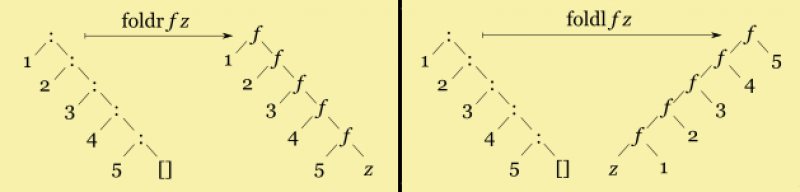
\includegraphics[max width=\textwidth]{:pp:fold-visualization.png}
\end{figure}
:


Tipurile acestor funcții sunt:


\begin{tcblisting}{ arc=0pt, outer arc=0pt, listing only, breakable}
Prelude> :t foldr
foldr :: (a -> b -> b) -> b -> [a] -> b
Prelude> :t foldl
foldl :: (a -> b -> a) -> a -> [b] -> a

\end{tcblisting}


\begin{tcolorbox}[colback=cyan!5, colframe=cyan!10, breakable]
Nu trebie să rețineți pe de rost tipurile. Încercați să înțelegeți ce exprimă și de ce sunt așa.
\end{tcolorbox}

Alte funcții de ordin superior des întâlnite: \texttt{map}, \texttt{filter}, \texttt{zipWith}, \texttt{flip}.


\subsection*{ Exerciții }

1. Fie două matrici reprezentate ca liste de liste. În rezolvarea exercițiilor de mai jos, puteți folosi doar funcții de ordin superior (împreună cu \texttt{take} și \texttt{drop}).

Implementați funcții care să returneze:

\begin{itemize}
	\item  linia \texttt{i} dintr-o matrice
	\item  elementul \texttt{(i, j)} dintr-o matrice
	\item  suma a două matrici
	\item  transpusa unei matrici 
	\item  produsul a două matrici
\end{itemize}


2. O imagine poate fi reprezentată ca o matrice de caractere (numiți, în continuare, "pixeli"). Considerăm că avem trei tipuri de pixeli: \texttt{'.'}, \texttt{'*'}, \texttt{' '}

Implementați următoarele funcții:
\begin{itemize}
	\item  flip orizontal, flip vertical, rotație de 90 în sens trigonometric și invers trigonometric
	\item  negativul (\texttt{'*'} si \texttt{'.'} devin \texttt{' '}, iar \texttt{' '} devine \texttt{'*'})
	\item  scalarea unei imagini cu \texttt{x} unități
	\item  alipirea a două imagini (cu aceeași înălțime) pe orizontală
	\item  alipirea a două imagini (cu aceeași lungime) pe verticală
	\item  crop orizontal de la de la coloana \texttt{x} la coloana \texttt{y}
	\item  crop vertical de la linia \texttt{x} la linia \texttt{y}
	\item  Implementați suprapunerea unei imagini peste o alta (având aceeași dimensiune)
\end{itemize}


\subsection*{ Resurse }

Puteți folosi următoarele pentru a vă testa funcțiile:


\begin{tcblisting}{ arc=0pt, outer arc=0pt, listing only, breakable}
l0="        ***** **            ***** **    "
l1="     ******  ****        ******  ****   "
l2="    **   *  *  ***      **   *  *  ***  "
l3="   *    *  *    ***    *    *  *    *** "
l4="       *  *      **        *  *      ** "
l5="      ** **      **       ** **      ** "
l6="      ** **      **       ** **      ** "
l7="    **** **      *      **** **      *  "
l8="   * *** **     *      * *** **     *   "
l9="      ** *******          ** *******    "
l10="      ** ******           ** ******     "
l11="      ** **               ** **         "
l12="      ** **               ** **         "
l13="      ** **               ** **         "
l14=" **   ** **          **   ** **         "
l15="***   *  *          ***   *  *          "
l16=" ***    *            ***    *           "
l17="  ******              ******            "
l18="    ***                 ***             "

img = [l0,l1,l2,l3,l4,l5,l6,l7,l8,l9,l10,l11,l12,l13,l14,l15,l16,l17,l18]

m1 = [[1, 2, 3], [4, 5, 6], [7, 8, 9]]
m2 = [[1, 0, 0], [0, 1, 1], [1, 0, 1]]

summ1m2 = [[2,2,3],[4,6,7],[8,8,10]]
prodm1m2 = [[4,2,5],[10,5,11],[16,8,17]]

-- functii care printeaza intr-un mod human-readable o matrice sau o imagine
display :: (Show a) => ([a] -> String) -> [[a]] -> IO ()
display displayLine = putStr . foldr (++) "" . map displayLine

-- folositi pentru a afisa o matrice de numere (ex. 1)
displayMat :: (Show a) => [[a]] -> IO ()
displayMat = display (foldr (\x acc -> show x ++ "   " ++ acc) "\n")

-- folositi pentru a afisa o "imagine" - matrice de siruri (ex. 2)
displayImg :: [String] -> IO ()
displayImg = display (++ "\n")


\end{tcblisting}

\section{ Course: Types in functional programming}
\section*{ Types in functional programming }

\subsection*{ Typing in programming languages }

\subsubsection*{ Strong vs weak typing }

Consider the following example from Javascript, where the operator \texttt{+} is applied on arguments of different types. The result is given below:

\begin{tcblisting}{ arc=0pt, outer arc=0pt, listing only, breakable}
[] + []  =  ""  
[] + {}  = "[object]"
{} + []  = 0
{} + {}  = null

\end{tcblisting}
 

where \texttt{[]} is the empty array and \texttt{\{\}} is the empty object. The result is quite surprising, and unpredictable. To explain it, we need to look at the implementation of the Javascript interpreter. In Javascript, there is a distinction between \textbf{primitive} and \textbf{non-primitive} values. Arrays (like \texttt{[]}) and objects (like \texttt{\{\}}) are considered non-primitive. Since the operation \texttt{+} is performed on primitive values, Javascript attempts to \textbf{convert} the operands to primitive. A pseudocode for this is shown below:

\begin{tcblisting}{ arc=0pt, outer arc=0pt, listing only, breakable}
     Convert(value) {
        if (value.valueOf() is a primitive) return it          //conversion to integer works?
        else if (value.toString() is a primitive) return it    //else convert to string, if possible 
             else error
     }

\end{tcblisting}


The conversion of \texttt{[]} to string yields the empty string, while the conversion of \texttt{\{\}} to string yields "[object]". This explains the first two results.

For the latter, we must know that \texttt{\{\}} can also be interpreted as a code-block, and this is the case here. Hence, the Javascript interpreter sees:

\begin{tcblisting}{ arc=0pt, outer arc=0pt, listing only, breakable} 
+ []
+ {}

\end{tcblisting}


where \texttt{+} is interpreted as a \textbf{unary} operator. JavaScript has such an implementation overloading for \texttt{+}. Without going into more details, \texttt{+ x} behaves like a \textit{conversion to Number} for x. Thus, \texttt{[]} converted to \texttt{Number} is \texttt{0}, while \texttt{\{\}} converted to \texttt{Number} is \texttt{NaN} (not a number).

\paragraph{ Morale }\hfill\\

The Javascript treatment of \texttt{+} is unimportant by itself, and it has some advantages for the programmer (although our example shows otherwise). However, we can note that, by allowing any \textbf{kind/type} of operand for \texttt{+}:
\begin{itemize}
	\item  \textbf{complicates the semantics} of the language (the programmer needs to known about conversion to primitives and conversion to numbers)
	\item  \textbf{reduces errors} (no Javascript error was signalled above), but \textbf{makes programs more prone to bugs}.
	\item  makes a program \textbf{more expressive} (\texttt{+} can be used in several ways) but sometimes difficult to use.
\end{itemize}


In programming language design, there is a fundamental tension between \textbf{expressiveness} and \textbf{typing}. Typing is a means for \textbf{enforcing constraints on what is deemed as a \textit{correct program}}. It may be the case that, \textit{conceptually correct} programs may not be accepted as \textbf{correct} from a typing perspective (this situation does seldom occur in Haskell).

A \textbf{strongly-typed} programming language, is more coercive with respect to \textbf{typing constraints}. In functional programming:
\begin{itemize}
	\item  Haskell
	\item  Scala
\end{itemize}
are considered \textbf{strongly-typed}. In imperative / OOP programming, the languages:
\begin{itemize}
	\item  Java
	\item  C++
	\item  Scala
\end{itemize}
are considered \textbf{strongly-typed}.

A \textbf{weakly-typed} programming language is more relaxed w.r.t. \textbf{typing constraints}. For instance, in functional programming:
\begin{itemize}
	\item  Racket (Lisp)
	\item  Clojure
\end{itemize}
are considered \textbf{weakly-typed}. In imperative / OOP programming, the languages:
\begin{itemize}
	\item  C
	\item  Python
	\item  PHP
	\item  Javascript
\end{itemize}

(and especially the latter) are considered weakly-typed. In the latter languages, types are usually reduced to primitive constructs (programmers cannot create new types), or the type construction procedure is very simplistic. For instance, in \texttt{Racket} (formerly known as \texttt{Scheme}), which weakly-typed:
\begin{itemize}
	\item  lists can hold any values (e.g.) \texttt{'(1 \#t "String")}, which means that the type for lists is \textbf{primitive} (not composed), and is simply \texttt{list}.
	\item  functions can return values of different types - the type for functions is also \textbf{primitive} - \texttt{\#procedure}. 
\end{itemize}

However, type verification is not absent in weakly-typed languages, including Racket/Scheme. For instance, the call \texttt{(+ 1 '())} will produce an error since the plus operator is called on values with invalid types.

We shall discuss Scheme/Racket in more detail later. It is worth noting that, in Racket there exists extensions (Typed Racket) which allow programmers to define and compose types to some extent.

The \textbf{weakly-typed} vs \textbf{strongly-typed} classification is not rigid and is subject to debate and discussion. There is no objective \textit{right-answer}. For instance, here, the language \texttt{C} is viewed as weakly-typed. We illustrate a small motivating example:


\begin{tcblisting}{ arc=0pt, outer arc=0pt, listing only, breakable}
int f (int x) {
    if (x != 0)
        return 1;
    return malloc(100);
}

\end{tcblisting}


In principle, the function \texttt{f} can return an integer, or a pointer to any object (of any type), and this is allowed by the compiler (which does issue a warning). Compared to, e.g. Java, this makes the \texttt{C} type system more relaxed.

There are valid arguments for considering \texttt{C} as strongly-typed and, as said before, there is no right answer.

\subsubsection*{ Compile-time vs runtime typing }

This classification is done w.r.t. \textbf{the moment} when type inference occurs:
\begin{itemize}
	\item  during the \textbf{compilation} of a program
	\item  at \textbf{runtime}
\end{itemize}

The former is also called \textbf{static typing}, while the latter - \textbf{dynamic typing}. In the literature, \textbf{static} and \textbf{dynamic} typing are also used with other meanings, hence, here, we prefer the terms \textbf{compile-time} and \textbf{runtime}.

The imperative/OOP languages:
\begin{itemize}
	\item  Java
	\item  Scala
	\item  C\textbackslash C++
\end{itemize}

perform compile-time type checking, as well as the functional languages:
\begin{itemize}
	\item  Haskell 
	\item  Scala
\end{itemize}

The imperative/OOP languages:
\begin{itemize}
	\item  Python
	\item  PHP
	\item  Javascript
\end{itemize}

perform runtime type checking, as well as the functional languages:
\begin{itemize}
	\item  Scheme/Racket (Lisp)
	\item  Clojure
\end{itemize}

Compile-time type checking is preferred for strongly-typed languages: the complexity of type verification is delegated to the compiler. Conversely, in weakly-typed languages, type verification is simpler, hence it can be performed by the interpreter, at runtime. Sometimes, a compiler may be absent. This is not a golden rule but merely an observation.

While runtime type checking is simpler to deploy, it has the disadvantage of not capturing typing bugs. Consider the following program in Racket:

\begin{tcblisting}{ arc=0pt, outer arc=0pt, listing only, breakable}
(define f (lambda (x) (if x 1 (+ 1 '()))))
(f #t)

\end{tcblisting}


The function receives a value \texttt{x} which must be a boolean. In the program above there is no error, even though \texttt{(+ 1 '())} is an incorrectly-typed function call. However, in the execution of the program (i.e. \texttt{(f \#t)}), the else branch of the function is not reached, hence no typing verification is performed.

Hence, runtime type checking only catches bugs \textbf{on the current program execution trace}.


\subsection*{ Typing in Haskell }

\subsection*{ Type inference in Haskell }

Haskell implements the \texttt{ Hindley-Milner type inference algorithm} \footnote{\url{https://en.wikipedia.org/wiki/Hindley\%E2\%80\%93Milner\_type\_system }}. In what follows, we present a simplified, and more easy-to-follow, but incomplete algorithm which serves as an illustration for the main concepts underlying the original one. 

\subsubsection*{ Intro }

Consider the following expressions, and their types:

\begin{tcblisting}{ arc=0pt, outer arc=0pt, listing only, breakable}
\x -> x + 1 :: Integer -> Integer
\x -> if x then 0 else 1 :: Bool -> Integer
zipWith (:) :: [a] -> [[a]] -> [[a]]
\f -> (f 1) + (f 2) :: (Integer -> Integer) -> Integer

\end{tcblisting}


We can see via the above example that types are constructed according to the following grammar:


\begin{tcblisting}{ arc=0pt, outer arc=0pt, listing only, breakable}
type ::= <const_type> | <type_var> | (<type>) | type -> type | [<type>]

\end{tcblisting}


This grammar only tells half the story regarding Haskell typing, however, for the purposes of this lecture, this view suffices. According to the above grammar, types can be:
\begin{itemize}
	\item  \textbf{constant types} (e.g. \texttt{Integer}, \texttt{String})
	\item  \textbf{type variables} (e.g. \texttt{a} - which are usually used to designate \textbf{any} possible type, as in \texttt{[a]})
	\item  \textbf{function types} (e.g. \texttt{Integer -\textgreater  Integer} or \texttt{(Integer -\textgreater  Integer)} if this type appears in a larger type expression)
	\item  \textbf{list types} (e.g. \texttt{[a]}).
	\item  any combination of the above rules.
\end{itemize}


\subsubsection*{ Expression trees }

We assume each Haskell expression is constructed via the following \textit{construction rules}:
\begin{itemize}
	\item  \textbf{functional application} (e.g. \texttt{take 2 [1,2,3]})
	\item  \textbf{function definition} (e.g. \texttt{\textbackslash x-\textgreater [x+1]})
\end{itemize}

We note that many Haskell definitions can be seen as such. For instance:

\begin{tcblisting}{ arc=0pt, outer arc=0pt, listing only, breakable}
g f = (f 1) + 1
<code>

can be seen as:

<code haskell>
g = \f -> (f 1) + 1

\end{tcblisting}


Hence, we can take any Haskell expression, and construct a \textbf{tree}, in which each node represents a \textbf{construction rule}, and children represent sub-expressions:
\begin{itemize}
	\item  for functional applications, the children are the \textbf{function name} and \textbf{the parameters}
	\item  for function definition, the children are \textbf{the variable/variables} and the \textbf{function body}.
\end{itemize}

For example, consider the expression tree for the function \texttt{g} shown previously (we use tabs to illustrate parent/child relationship):

\begin{tcblisting}{ arc=0pt, outer arc=0pt, listing only, breakable}
\f -> (f 1) + 1
  f
  (f 1) + 1
    (+)
    (f 1)
       f 
       1
    1

\end{tcblisting}


In what follows, we shall use expression trees to perform type inference.

\subsubsection*{ Typing rules }

We introduce the following \textbf{typing rules}:

\paragraph{ Rule (TVar) }\hfill\\

If \texttt{v} is bound to a constant expression e of type \texttt{ct}, then \texttt{v :: ct}

\paragraph{ Rule (TFun) }\hfill\\

If \texttt{x :: t1} and \texttt{e :: t2} then \texttt{\textbackslash x -\textgreater  e  :: t1 -\textgreater  t2}

\paragraph{ Rule (TApp) }\hfill\\

If \texttt{f :: t1 -\textgreater  t2} and \texttt{e :: t1} then \texttt{(f e) :: t2}

The above rule can be naturally generalised:

If \texttt{f :: t1 -\textgreater  t2 -\textgreater  ... -\textgreater  tn -\textgreater  t} and \texttt{e1 :: t1}, ..., \texttt{en :: tn} then \texttt{(f e1 ... en) :: t}

In what follows, we will use these rules to make judgements on our types. These rules have a twofold usage:
\begin{itemize}
	\item  \textbf{deduce} the type of an expression, based on \textit{existing knowledge}
	\item  \textbf{make hypotheses} regarding the type of an expression (we shall not focus on this aspect in the presentation))
\end{itemize}

\subsubsection*{ Type inference stage 1: Expression tree construction }

Type inference for an expression \texttt{e} can be seen as having two stages. In the first stage, we:
\begin{itemize}
	\item  construct the expression tree of \texttt{e}
	\item  make \textbf{hypotheses} regarding the types of \textbf{yet untyped} expressions (e.g. variables).
\end{itemize}

We illustrate the first stage on the previous definition of \texttt{g}:


\begin{tcblisting}{ arc=0pt, outer arc=0pt, listing only, breakable}
\f -> (f 1) + 1 :: ?
  f :: tf (here we introduce tf as the type of f. This is a type hypothesis)
  (f 1) + 1 :: ?
    (+) :: ?
    (f 1) :: ?
       f :: t1 -> t2 (this is another hypothesis, stemming from the fact that f is applied on 1)
       1 :: ?
    1 :: ?

\end{tcblisting}


\subsubsection*{ Type inference stage 2: Rule application }

In this stage, we start from the previously-build tree, and:
\begin{itemize}
	\item  \textbf{apply typing rules} to deduce types for new sub-expressions
	\item  \textbf{perform type unification}: This is one aspect that we shall not elaborate on, in this lecture. 
\end{itemize}

This is equivalent to a \textbf{bottom-up} tree traversal: We start from the leaves, and progress to the root (i.e. the expression to be typed).

Without delving into details, \textbf{type unification} is an important ingredient, because it allows us to infer \textbf{the most general} type of an expression. Consider the following Haskell expression: \texttt{\textbackslash f x -\textgreater  (f x,f 1)}, which defines a function that takes another function \texttt{f}, a value \texttt{x} and returns a pair: the first element of the pair is the application \texttt{f x}, while the second - \texttt{f 1}:
\begin{itemize}
	\item  initially, we do not know what \texttt{f} is, hence it has \textbf{the most general type} (say) \texttt{tf} - it can be anything;
	\item  judging by the application \texttt{f x}, we deduce that \texttt{f} must be a function, of type \texttt{a-\textgreater b}, where \texttt{x::a}
	\item  judging by the application \texttt{f 1}, we deduce that \texttt{a} must be an \texttt{Integer}
\end{itemize}
The unification process combines the information collected so far:
\begin{itemize}
	\item  \texttt{tf} must unify (coincide with) \texttt{a -\textgreater  b}
	\item  \texttt{a} must unify with \texttt{Integer}
\end{itemize}

The final type for the expression is: \texttt{(Integer -\textgreater  b) -\textgreater  Integer -\textgreater  (b, b)}

We illustrate the second stage of the type inference on the same example:


\begin{tcblisting}{ arc=0pt, outer arc=0pt, listing only, breakable}
\f -> (f 1) + 1 :: tf -> Integer
  f :: tf (via (TFun))
  (f 1) + 1 :: Integer (via (TApp))
    (+) :: Integer -> Integer -> Integer (this we know from Prelude, after the type synthesis of (+), also t2 must unify with Integer)
    (f 1) :: t2 (via (TApp); also, t1 must unify with Integer)
       f :: t1 -> t2
       1 :: Integer (via (TVar), from Prelude)
    1 :: Integer (via (TVar), from Prelude)

\end{tcblisting}


The (pseudo)-algorithmic procedure concludes with the following answer:
\begin{itemize}
	\item  \texttt{g :: tf -\textgreater  Integer}, where

  \begin{itemize}
  	\item  \texttt{tf} unifies with \texttt{t1 -\textgreater  t2}
  	\item  \texttt{t2} unifies with \texttt{Integer}
  	\item  \texttt{t1} unifies with \texttt{Integer}
  \end{itemize}
\end{itemize}

After unification, the result is shown to the programmer: \texttt{ g :: (Integer -\textgreater  Integer) -\textgreater  Integer}

Exercises. Find the type of the following expressions, by applying the type synthesis pseudo-algorithm:
\begin{itemize}
	\item  \texttt{map (\textbackslash x-\textgreater [x+1])}
	\item  \texttt{\textbackslash f x-\textgreater  if x then f x else x}
	\item  \texttt{g f x = x \&\& (f x)}
	\item  \texttt{g f = f (g f)}
\end{itemize}


\section{ Course: Abstract datatypes}
\subsection*{ Abstract Datatypes }

\subsubsection*{ Intro }

An Abstract Datatype relies on \textit{functions} to describe the possible values of a type. We start with a simplistic example:


\begin{tcblisting}{ arc=0pt, outer arc=0pt, listing only, breakable}
data Nat = Zero | Succ Nat

\end{tcblisting}

\begin{itemize}
	\item  the expression \texttt{data Nat} introduces a new \textbf{type} in the programming language
	\item  after \texttt{=}, the \textbf{base constructors} of the type follow. In Haskell, \textbf{all constructors} must begin with a capital letter
	\item  \texttt{Zero} is a nullary constructor. 
	\item  \texttt{Succ Nat} designates an \textbf{internal} constructor, which expects a natural number (of type \texttt{Nat}). A value \texttt{(Succ x)} \textbf{is} of type \texttt{Nat} (i.e. a natural number), and we may be tempted to see it as a function call, which \textit{returns} the successor of \texttt{x}
\end{itemize}

\texttt{Zero} and \texttt{Succ} are called \textbf{data constructors} in Haskell. \texttt{Nat} is called a \texttt{type} or \texttt{type-constructor}. We shall distinguish between the two in a later lecture.

Note that the \textit{internal} representation of an ADT, as perceived by the programmer, is \textit{abstract}. We may see values as \textit{calls} of special functions - data constructors. Except for their meaning (and language-level implementation), data constructors behave exactly as functions. For instance:
\begin{itemize}
	\item  \texttt{Zero :: Nat}
	\item  \texttt{Succ :: Nat -\textgreater  Nat}
\end{itemize}

We continue the example with addition:


\begin{tcblisting}{ arc=0pt, outer arc=0pt, listing only, breakable}
add :: Nat -> Nat -> Nat
add Zero y = y
add (Succ x) y = Succ (add x y)

\end{tcblisting}


An important observation is that the \textbf{pattern matching mechanism} in Haskell relies on data constructors, and their applications. For instance, the following definition is a correct usage of the pattern matching mechanism:

\begin{tcblisting}{ arc=0pt, outer arc=0pt, listing only, breakable}
f (1:y:[]) = ...

\end{tcblisting}

I uses the data constructors \texttt{(:)} and \texttt{[]} for lists, as well as the data constructor \texttt{1} for integers. The pattern describes any list of integers which starts with a \texttt{1} and contains exactly two elements.

\subsubsection*{ Monomorphic List implementation }

In what follows, we give an implementation for the type \textit{List of integers}. This type is called \textit{monomorphic}, since our list can only contain elements of a single type (integer):


\begin{tcblisting}{ arc=0pt, outer arc=0pt, listing only, breakable}
data IList = Void | Cons Integer IList

app :: IList -> IList -> IList
app Void l = l
app (Cons h t) l = Cons h (app t l)

convert :: IList -> [Integer]
convert Void = []
convert (Cons h t) = h : (convert t)

mfoldl :: (b -> Integer -> b) -> b -> IList -> b
mfoldl op acc Void = acc
mfoldl op acc (Cons h t) = mfoldl op (op acc h) t

mfoldr :: (Integer -> a -> a) -> a -> IList -> a
mfoldr op acc Void = acc
mfoldr op acc (Cons h t) = op h (mfoldr op acc t)

convert2 :: IList -> [Integer]
convert2 = mfoldr (:) []

showl :: IList -> String
showl = show . convert2


\end{tcblisting}


In the above code, we have defined some basic list operations, such as \texttt{app} (list concatenation) and \texttt{convert}, which transforms a list of type \texttt{IList} to a conventional Haskell list (of type \texttt{[Integer]}).

We have also implemented the two folding procedures for \texttt{IList}. Note the type signature of each fold. Finally, we have used folds to provide an alternative implementation for convert, as well as for converting lists to strings.


\subsubsection*{ Propositional Logic in Haskell }

Abstract Datatypes are a natural way to define more elaborate data-structures, such as propositional formulae. We give a possible definition below:


\begin{tcblisting}{ arc=0pt, outer arc=0pt, listing only, breakable}
data Formula = Var String | And Formula Formula | Or Formula Formula | Not Formula

\end{tcblisting}


We observe that:
\begin{itemize}
	\item  \texttt{Var :: String -\textgreater  Formula}
	\item  \texttt{And :: Formula -\textgreater  Formula -\textgreater  Formula}
	\item  \texttt{Or :: Formula -\textgreater  Formula -\textgreater  Formula}
	\item  \texttt{Not :: Formula -\textgreater  Formula}
\end{itemize}

A good exercise consists in the implementation of a display function for formulae:

\begin{tcblisting}{ arc=0pt, outer arc=0pt, listing only, breakable}
fshow :: Formula -> String
fshow (Var v) = v
fshow (And f1 f2) = "("++(fshow f1)++" ^ "++(fshow f2)++")"
fshow (Or f1 f2) = "("++(fshow f1)++" V "++(fshow f2)++")"
fshow (Not f) = "~("++(fshow f)++")"

\end{tcblisting}


Next, we implement a function \texttt{push}, which pushes negation \textit{inward}:

\begin{tcblisting}{ arc=0pt, outer arc=0pt, listing only, breakable}
push :: Formula -> Formula
push (Var v) = (Var v)
push (Not (Var v)) = Not (Var v)
push (Not (And f1 f2)) = Or (push (Not f1)) (push (Not f2))
push (Not (Or f1 f2)) = And (push (Not f1)) (push (Not f2))
push (And f1 f2) = And (push f1) (push f2)
push (Or f1 f2) = Or (push f1) (push f2)

\end{tcblisting}


Notice, at lines 4,5 the implementation of deMorgan's laws.

Finally, we implement a function which computes the truth-value of a formula, under a certain interpretation. First, we define the type \texttt{Interpretation}:

\begin{tcblisting}{ arc=0pt, outer arc=0pt, listing only, breakable}
type Interpretation = String -> Bool

i :: Interpretation
i "x" = True
i "y" = False
i "z" = True

\end{tcblisting}
 

In the first line, we have defined a \textbf{type-alias}: \texttt{Interpretation} is a function from strings to booleans. We have also implemented a three-variable interpretation, for testing purposes. Next, we implement \texttt{eval}:


\begin{tcblisting}{ arc=0pt, outer arc=0pt, listing only, breakable}
eval :: Interpretation -> Formula -> Bool
eval i (Var v) = i v
eval i (Not f) = not(eval i f)
eval i (And f1 f2) = (eval i f1) &\&&&\&& (eval i f2)
eval i (Or f1 f2) = (eval i f1) || (eval i f2)

\end{tcblisting}


\subsubsection*{ Monomorphic Trees in Haskell }


\begin{tcblisting}{ arc=0pt, outer arc=0pt, listing only, breakable}
data ITree = Leaf | Node ITree Integer ITree

\end{tcblisting}


Note that:
\begin{itemize}
	\item  \texttt{Leaf :: ITree}
	\item  \texttt{Node :: ITree -\textgreater  Integer -\textgreater  ITree -\textgreater  ITree}
\end{itemize}

Next, we implement a folding operation on Trees. The key to it is to conceptually define what folding should do on Trees. To grasp an intuition, recall that: 
\begin{itemize}
	\item  \texttt{foldr (:) []} is the \textbf{identity function} on lists. Hence, \texttt{foldr (:) [] [1,2,3]} produces \texttt{[1,2,3]}.
	\item  also, recall that the map operation can be defined as: \texttt{\textbackslash f -\textgreater  foldr ((:).f) []}
\end{itemize}

Similar to the list case, a fold on trees should:
\begin{itemize}
	\item  \textbf{preserve the tree structure}, given the appropriate operator (e.g. \texttt{Node}). 
	\item  hence, the call \texttt{mtfold Node Leaf} (where \texttt{Leaf} is the accumulator) should be the \textbf{identity function on trees}. 
\end{itemize}

Let us define the identity function \texttt{tid} for trees:

\begin{tcblisting}{ arc=0pt, outer arc=0pt, listing only, breakable}
tid Leaf = Leaf
tid (Node r k l) = Node (tid r) k (tid l)

\end{tcblisting}


As already said, \texttt{(tid t)} is equivalent to the call \texttt{(mtfold Node Leaf t)}, for any arbitrary tree \texttt{t}.
To obtain the general \texttt{mtfold} implementation, we simply generalise \texttt{Node} by an arbitrary operation \texttt{op}:
\begin{itemize}
	\item  if \texttt{Node :: ITree -\textgreater  Integer -\textgreater  ITree -\textgreater  ITree}, then
	\item  \texttt{op :: b -\textgreater  Integer -\textgreater  b -\textgreater  b}
\end{itemize}

We also generalise \texttt{Leaf} by an arbitrary accumulator:
\begin{itemize}
	\item  if \texttt{Leaf :: ITree} then
	\item  \texttt{acc :: b}
\end{itemize}

The code generalisation becomes:


\begin{tcblisting}{ arc=0pt, outer arc=0pt, listing only, breakable}
mtfold :: (b -> Integer -> b -> b) -> b -> ITree -> b
mtfold op acc = 
    let f (Node left key right) = f (f left) key (f right)
        f Leaf = acc
    in f

\end{tcblisting}


Notice that \texttt{f} is precisely the generalisation of \texttt{tid} according to our observations. We can use \texttt{mtfold} to implement various tree operations such as:


\begin{tcblisting}{ arc=0pt, outer arc=0pt, listing only, breakable}
tsum = mtfold (\k r l->k + r + l) 0 
tmirror = mtfold (\k r l -> Node l k r) Leaf 
tflatten = mtfold (\k r l -> r ++ [k] ++ l) [] 

\end{tcblisting}
 
\subsection{ Lab: Abstract datatypes}
\section*{ Tipuri de date abstracte }

Scopul laboratorului:
\begin{itemize}
	\item  Recapitularea conceptului de TDA
	\item  Definirea de TDA-uri în Haskell
	\item  Familiarizarea cu conceptul de TDA-uri polimorfice
	\item  Introducerea tipului de date \texttt{Maybe}
\end{itemize}


\subsection*{ Tipuri de date abstracte (TDA) }

\textbf{Tipurile de date abstracte} sunt modele pentru a defini tipuri de date în funcție de comportamentul acestora (valori posibile, axiome, operații), contrastând cu \textit{structurile de date}, definite din punct de vedere al implementării.

Un TDA familiar este \textbf{list}. \\Pentru a lucra cu liste într-un limbaj ca Java, am scris două \textit{implementări} distincte, și anume \texttt{LinkedList} și \texttt{ArrayList}. Ambele implementări respectă specificațiile din primul paragraf.

\begin{tcolorbox}[colback=yellow!40, colframe=yellow!60, breakable]
Unii autori includ în descrierea TDA-urilor și complexități. Din acest punct de vedere, implementările 
\texttt{LinkedList} și \texttt{ArrayList} diferă.
\end{tcolorbox}


\subsubsection*{ Constructori }

Valorile posibile ale unui TDA sunt date de constructorii acestuia.\\Să considerăm un tip simplu de date: \texttt{Bool}, care poate avea două valori: \texttt{False} și \texttt{True}.\\Sintaxa Haskell pentru a defini acest tip de date este următoarea:


\begin{tcblisting}{ arc=0pt, outer arc=0pt, listing only, breakable}
data Bool = False | True

\end{tcblisting}


\begin{tcolorbox}[colback=yellow!40, colframe=yellow!60, breakable]
Atât numele tipului de date cât și numele constructorilor trebuie scris cu literă mare.
\end{tcolorbox}

\texttt{False} și \texttt{True} nu sunt parametrizate și pot fi privite ca valori. Se mai numesc și \textit{constructori nulari}.\\
Să considerăm un alt TDA care descrie un arbore binar cu valori întregi. Arborele poate fi gol sau un nod cu doi copii.


\begin{tcblisting}{ arc=0pt, outer arc=0pt, listing only, breakable}
data Tree = Nil | Node Int Tree Tree

\end{tcblisting}


\texttt{Node} este un constructor care primește un argument de tipul \texttt{Int} și două argumente de tip \texttt{Tree}, pentru a creea o valoare de tip \texttt{Tree}. Putem să ne gândim la el ca la o funcție:


\begin{tcblisting}{ arc=0pt, outer arc=0pt, listing only, breakable}
Prelude> :t Node
Node :: Int -> Tree -> Tree -> Tree

\end{tcblisting}


Constructorii sunt foarte importanți în \textit{pattern matching}. Ca exemplu, vom scrie o funcție care însumează toate valorile dintr-un arbore:


\begin{tcblisting}{ arc=0pt, outer arc=0pt, listing only, breakable}
treeSum :: Tree -> Int
treeSum Nil = 0
treeSum (Node v l r) = v + (treeSum l) + (treeSum r)

\end{tcblisting}


Observăm prezența a două pattern-uri: unul pentru arborele vid, celălalt pentru un nod, într-un fel foarte asemănător cu modul în care lucram cu liste, făcând pattern matching pe \texttt{[]} și \texttt{(x:xs)}.

\begin{tcolorbox}[colback=cyan!5, colframe=cyan!10, breakable]
Observați că ghci nu știe cum să afișeze arborele nostru:


\begin{tcblisting}{ arc=0pt, outer arc=0pt, listing only, breakable}
Prelude> Node 1 Nil Nil

<interactive>:38:1:
    No instance for (Show Tree) arising from a use of 'print'
    In a stmt of an interactive GHCi command: print it

\end{tcblisting}


Pentru a vă fi mai ușor să vă verificați, puteți obține o reprezentare a tipurilor definite de voi astfel:


\begin{tcblisting}{ arc=0pt, outer arc=0pt, listing only, breakable}
data Tree = Nil | Node Int Tree Tree deriving (Show)

\end{tcblisting}


Pe scurt, acest lucru înrolează TDA-ul vostru în clasa \texttt{Show}, oferind o implementare implicită a funcției \texttt{show} (apelată de ghci). Mai multe detalii în laboratorul următor.


\begin{tcblisting}{ arc=0pt, outer arc=0pt, listing only, breakable}
Prelude> Node 1 Nil Nil
Node 1 Nil Nil

\end{tcblisting}

\end{tcolorbox}


\subsubsection*{ Înregistrări }

Vrem să definim un TDA pentru a descrie un student, folosind următoarele câmpuri: nume, prenume, an de studiu, medie.


\begin{tcblisting}{ arc=0pt, outer arc=0pt, listing only, breakable}
-- tipul de date si constructorul au acelasi nume, ceea ce este ok
-- pentru ca reprezinta concepte diferite.
data Student = Student String String Int Float

\end{tcblisting}


Observăm că semnficația câmpurilor nu este evidentă din definiție. Vrem să extragem valori dintr-un Student; definim funcțiile:


\begin{tcblisting}{ arc=0pt, outer arc=0pt, listing only, breakable}
nume :: Student -> String
nume (Student n _ _ _) = n

prenume :: Student -> String
prenume (Student _ p _ _) = p

an :: Student -> Int
an (Student _ _ a _) = a

medie :: Student -> Float
medie (Student _ _ _ m) = m

\end{tcblisting}


Pentru a face descrierea tipului de date mai clară și a evita să scriem manual acele funcții, putem folosi sintaxa:


\begin{tcblisting}{ arc=0pt, outer arc=0pt, listing only, breakable}
data Student = Student { nume :: String
                       , prenume :: String
                       , an :: Int
                       , medie :: Float
                       }

\end{tcblisting}

                      


\subsection*{ TDA-uri polimorfice }

Până acum, am definit TDA-uri care lucrează doar cu întregi. Dorim să scăpăm de această limitare și să definim TDA-uri care pot lucra cu orice alt tip de date. De exemplu, are sens să considerăm capul unei liste care conține elemente de tip \texttt{a}, ca fiind un element de tip \texttt{a}, indiferent de cum arată acest tip.\\
Într-adevăr, aceasta este definiția funcției \texttt{head} existentă în Haskell:


\begin{tcblisting}{ arc=0pt, outer arc=0pt, listing only, breakable}
Prelude> :t head
head :: [a] -> a

\end{tcblisting}


\texttt{a} se numește \textbf{variabilă de tip} și poate să reprezinte orice tip de date (evident, cu condiția ca toate \texttt{a}-urile care apar să se refere la același tip).

\begin{tcolorbox}[colback=blue!10, colframe=blue!20]
Să ne uităm la tipul altei funcții cunoscute:


\begin{tcblisting}{ arc=0pt, outer arc=0pt, listing only, breakable}
Prelude> :t map
map :: (a -> b) -> [a] -> [b]

\end{tcblisting}


\texttt{map} primește ca argument o funcție - care primește un element de tip \texttt{a} și întoarce un element de tip \texttt{b} - și o listă de elemente de tip \texttt{a} și întoarce o listă de elemente de tip \texttt{b}. De precizat că \texttt{a} și \texttt{b} pot fi distincte dar nu este necesar.
\end{tcolorbox}

Listele din Haskell sunt \textbf{polimorfice}. Ele pot conține date de orice tip. O instanță a listelor are însă un tip concret:


\begin{tcblisting}{ arc=0pt, outer arc=0pt, listing only, breakable}
Prelude> :t ['a', 'b', 'c']
['a', 'b', 'c'] :: [Char]

\end{tcblisting}


\subsubsection*{ Constante polimorfice }

Care este tipul listei vide?


\begin{tcblisting}{ arc=0pt, outer arc=0pt, listing only, breakable}
Prelude> :t []
[] :: [a]

\end{tcblisting}


Observăm că tipul listei vide este general. Asta înseamnă că lista vidă poate fi tratată ca o listă de orice tip.


\begin{tcblisting}{ arc=0pt, outer arc=0pt, listing only, breakable}
Prelude> [1,2,3] ++ "123" -- eroare, tipuri diferite
Prelude> [1,2,3] ++ []
[1,2,3]
Prelude> "123" ++ []
"123"

\end{tcblisting}


Spunem că \texttt{[]} este o \textbf{constantă polimorfică}.

\begin{tcolorbox}[colback=blue!10, colframe=blue!20]
O altă constantă polimorfică este, de exemplu \texttt{1}. De aceea putem scrie:


\begin{tcblisting}{ arc=0pt, outer arc=0pt, listing only, breakable}
Prelude> 1 + 2
3
Prelude> 1 + 2.71
3.71

\end{tcblisting}


Dacă forțăm 1 să fie întreg, vom primi o eroare la a doua adunare:

\begin{tcblisting}{ arc=0pt, outer arc=0pt, listing only, breakable}
Prelude> (1 :: Int) + 2.71

<interactive>:60:14:
    No instance for (Fractional Int) arising from the literal '2.71'
    In the second argument of '(+)', namely '2.71'
    In the expression: (1 :: Int) + 2.71
    In an equation for 'it': it = (1 :: Int) + 2.71

\end{tcblisting}


\texttt{1} are însă o constrângere despre care vom discuta în laboratorul următor.
\end{tcolorbox}


Pentru a implementa în Haskell un TDA polimorfic, folosim sintaxa:


\begin{tcblisting}{ arc=0pt, outer arc=0pt, listing only, breakable}
data List a = Empty | Cons a (List a)

\end{tcblisting}


\begin{tcolorbox}[colback=blue!10, colframe=blue!20]
Ce este \texttt{List}?\\
\texttt{List} este un \textbf{constructor de tip}, nu un tip de date. Constructorii de tip primesc ca parametrii \textit{tipuri} și întorc un tip (sau un alt constructor de tip dacă nu primesc suficienți parametrii).\\Asta înseamnă că, \texttt{List} nu este un \textit{tip}, dar \texttt{List Int}, \texttt{List Char} etc. sunt tipuri.
\end{tcolorbox}

\subsubsection*{ Maybe și Either }

Unul dintre TDA-urile puse la dispoziție de Haskell este \texttt{Maybe}, un tip \textit{polimorfic} care modelează prezența unei anumite valori, sau absența acesteia:

\begin{tcblisting}{ arc=0pt, outer arc=0pt, listing only, breakable}
data Maybe a = Nothing | Just a

\end{tcblisting}


Pentru a ilustra importanța acestui TDA, considerăm următoare situație: vrem să implementăm o funcție care returnează suma valoriilor celor doi copii ai unui nod dat:


\begin{tcblisting}{ arc=0pt, outer arc=0pt, listing only, breakable}
childrenSum :: Tree -> Maybe Int
childrenSum Nil = Nothing
childrenSum (Node _ Nil _) = Nothing
childrenSum (Node _ _ Nil) = Nothing
childrenSum (Node _ (Node v _ _) (Node w _ _)) = Just (v + w)

\end{tcblisting}


Această sumă există doar pentru arbore diferit de Nil, cu ambii copii diferiți de Nil.

Putem scrie o funcție care ia un \texttt{Maybe} și returnează un șir pentru printare. Combinăm apoi cele două funcții:


\begin{tcblisting}{ arc=0pt, outer arc=0pt, listing only, breakable}
pretty :: Maybe Int -> String
pretty Nothing = "No value"
pretty (Just v) = "Sum is " ++ show v

printChildrenSum :: Tree -> String
printChildrenSum = pretty . childrenSum

\end{tcblisting}


Încărcăm modulele în ghci și voilà:

\begin{tcblisting}{ arc=0pt, outer arc=0pt, listing only, breakable}
*Main> printChildrenSum (Node 1 (Node 1 Nil (Node 2 Nil Nil)) (Node 3 (Node 4 (Node 5 Nil Nil) Nil) (Node 6 Nil Nil)))
"Sum is 4"
*Main> printChildrenSum Nil
"No value"
*Main> printChildrenSum (Node 1 Nil (Node 1 Nil Nil))
"No value"
*Main> printChildrenSum (Node 1 (Node 1 Nil Nil) Nil)
"No value"

\end{tcblisting}


Un TDA similar este \texttt{Either}, care modelează valori cu două tipuri posibile:


\begin{tcblisting}{ arc=0pt, outer arc=0pt, listing only, breakable}
data Either a b = Left a | Right b

\end{tcblisting}


Prin convenție, constructorul \texttt{Left} reprezintă o eroare, iar constructorul \texttt{Right} o valoare corectă. Astfel putem extinde mecanisme de error-handling pentru a conține mai multe informații despre ce a cauzat eroarea (spre deosebire de \texttt{Maybe}, care doar indică \textbf{existența} unei erori):


\begin{tcblisting}{ arc=0pt, outer arc=0pt, listing only, breakable}
childrenSum :: Tree -> Either String Int
childrenSum Nil = Left "Tree is Nil"
childrenSum (Node _ Nil _) = Left "Left child is Nil"
childrenSum (Node _ _ Nil) = Left "Right child is Nil"
childrenSum (Node _ (Node v _ _) (Node w _ _)) = Right (v + w)

pretty :: Either String Int -> String
pretty (Left s) = s
pretty (Right i) = "Sum is " ++ show i

printChildrenSum :: Tree -> String
printChildrenSum = pretty . childrenSum

\end{tcblisting}



\begin{tcblisting}{ arc=0pt, outer arc=0pt, listing only, breakable}
*Main> printChildrenSum (Node 1 (Node 1 Nil (Node 2 Nil Nil)) (Node 3 (Node 4 (Node 5 Nil Nil) Nil) (Node 6 Nil Nil)))
"Sum is 4"
*Main> printChildrenSum Nil
"Tree is Nil"
*Main> printChildrenSum (Node 1 Nil (Node 1 Nil Nil))
"Left child is Nil"
*Main> printChildrenSum (Node 1 (Node 1 Nil Nil) Nil)
"Right child is Nil"

\end{tcblisting}


\subsubsection*{ Exerciții }

\begin{tcolorbox}[colback=yellow!40, colframe=yellow!60, breakable]
Încercați să vă obișnuiți să scrieți explicit tipurile tuturor funcțiilor definite de voi în continuare.
\end{tcolorbox}

\subparagraph{ 1. List }\hfill\\

a) implementați TDA-ul pentru propria voastră listă care poate conține doar numere întregi\\b) scrieți o funcție care convertește valori ale TDA-ului vostru în liste din Haskell

\begin{tcolorbox}[colback=cyan!5, colframe=cyan!10, breakable]
Dacă tipul vostru de listă se numește \texttt{List}, atunci tipul funcției va fi: 


\begin{tcblisting}{ arc=0pt, outer arc=0pt, listing only, breakable}
convertList :: List -> [Int]

\end{tcblisting}

\end{tcolorbox}

c) modificați tipul \texttt{List} pentru a fi polimorfic, apoi modificați și funcția \texttt{convertList}

\subparagraph{ 2. Tree }\hfill\\
a) Implementați TDA-ul pentru arbori polimorfici.\\b) Implementați \texttt{foldT}, echivalentul lui \texttt{foldr} (puteți vizualiza rezultatul ca fiind înlocuirea tuturor constructorilor nulari cu o valoare constantă și a tuturor celorlalți constructori cu funcții care iau același numă de argumente.\\c) Implementați o funcție \texttt{mapT} (echivalentul lui \texttt{map}), folosindu-vă de \texttt{foldT}.\\d) Implementați o funcție \texttt{zipWithT} (echivalentul lui \texttt{zipWith}).\\
\subparagraph{ 3. Numere naturale extinse }\hfill\\
a) Implementați un TDA care să modeleze numere naturale extinse cu un punct la infinit ($ \hat{\mathbb{N}} = \mathbb{N} \cup \{ \infty \}$).\\b) Implementați o funcție \texttt{extSum} care să evalueze suma a două numere naturale extinse.\\c) Implementați o funcție \texttt{extDiv} care să evalueze raportul a două numere naturale extinse (împărțirea la 0 și la infinit are rezultat definit).\\d) Implementați o funcție \texttt{extLess} care spune dacă un număr natural extins e mai mic decât un altul.

În laboratorul următor, vom vedea cum putem implementa aceste operații într-un mod consistent cu restul limbajului, folosind operatori cunoscuți (\texttt{+}, \texttt{div}, \texttt{\textless }).
                   
\subparagraph{ 4. Înregistrări }\hfill\\

a) Scrieți un TDA care codifică un tuplu (înregistrare) format din următoarele câmpuri:
   \begin{itemize}
   	\item  Nume (codificat ca String)
   	\item  Vârstă (codificat ca Integer)
   	\item  Prieteni (codificat ca o lista de String-uri)
   	\item  Notă PP (codificat ca Integer). Acest câmp este opțional!
   \end{itemize}

b) Scrieți o funcție care primește o listă de înregistrări și le întoarce pe acelea pentru care vârsta este mai mare ca 20.\\c) Scrieți o funcție care primește o listă de înregistrări și le întoarce pe acelea care conțin cel puțin un prieten cu numele "Matei".\\d) Scrieți o funcție care primește o listă de înregistrări și le întoarce pe acelea care conțin câmpul "Notă PP".\\e) Scrieți o funcție care primește o listă de nume, o listă de vârste, o listă ce conține liste de prieteni, și întoarce o listă de înregistrări corespunzătoare.

\subsection*{ Referințe }

\begin{itemize}
	\item  \texttt{Abstract Data Type - Haskell wiki} \footnote{\url{https://wiki.haskell.org/Abstract\_data\_type}}
	\item  \texttt{Algebraic Data Type - Haskell wiki} \footnote{\url{https://wiki.haskell.org/Algebraic\_data\_type}}
	\item  \texttt{Maybe - Haskell wiki} \footnote{\url{https://wiki.haskell.org/Maybe}}
\end{itemize}

\section{ Course: Polymorphism in functional languages}
\section*{ Polymorphism in functional languages }

\subsection*{ Polymorphism in Object-Oriented languages }

Translated literally, the term \textbf{polymorphism} means \textbf{multiple shapes}. Polymorphism in programming languages is a powerful modularisation tool, which allows programmers to:
\begin{itemize}
	\item  \textbf{abstract from implementation details} (in the case of ad-hoc polymorphism)
	\item  \textbf{define a unique implementation for a range of types} (in the case of parametric polymorphism / genericity)
\end{itemize}

Polymorphism is a mechanism supported by virtually any strongly-typed programming language, including functional and object-oriented ones.

\subsubsection*{ Ad-hoc polymorphism }

In an Object-Oriented language (say, Java), \textbf{ad-hoc polymorphism} allows the programmer to \textit{(dynamically) select the implementation of a function, based on the type(s) of the variable(s) on which the former is applied}.

Consider the following class definitions:

\begin{tcblisting}{ arc=0pt, outer arc=0pt, listing only, breakable}
class Animal {
  public void talk (){
    System.out.println("I am an Animal");
  }
}

class Bird extends Animal {
  public void talk (){
    System.out.println("Cip-cirip");
  }
}

\end{tcblisting}


Finally, consider the following code:

\begin{tcblisting}{ arc=0pt, outer arc=0pt, listing only, breakable}
 Animal [] v = new Animal [2];
    v[0] = new Animal();
    v[1] = new Bird();
    for (Animal a:v)
      a.talk();

\end{tcblisting}


whose output is:

\begin{tcblisting}{ arc=0pt, outer arc=0pt, listing only, breakable}
I am Animal
Cip-cirip

\end{tcblisting}


The example illustrates \textbf{ad-hoc polymorphism}, or \textbf{method overriding}:
\begin{itemize}
	\item  the \texttt{talk} method from the class \texttt{Animal} has been overridden in the class \texttt{Bird} which extends \texttt{Animal}.
	\item  moreover, establishing the implementation of \texttt{a.talk()} is done \textbf{at runtime}, based on the \textbf{actual} (here \texttt{Bird}) \textbf{not declared} (\texttt{Animal}) type of \texttt{a}.
\end{itemize}

Method overriding should not be confused with \textbf{method overloading} which means that the same function name can be used for different function implementations, each having a different signature. The following code, which continues the previous example, illustrates \textbf{overloading}:


\begin{tcblisting}{ arc=0pt, outer arc=0pt, listing only, breakable}
  public void listen_to(Animal a){
    System.out.println("An animal is listening:");
    a.talk();
  }
  public void listen_to(Bird b){
    System.out.println("A bird is listening:");
    b.talk();
  }

\end{tcblisting}

The function \texttt{listen\_to} has been overloaded. Now, consider the calls:

\begin{tcblisting}{ arc=0pt, outer arc=0pt, listing only, breakable}
listen_to(v[0]);
listen_to(v[1]); 
listen_to(new Bird());

\end{tcblisting}


The output is:

\begin{tcblisting}{ arc=0pt, outer arc=0pt, listing only, breakable}
An animal is listening:
I am an Animal
An animal is listening:
Cip-cirip
A bird is listening:
Cip-cirip

\end{tcblisting}


The interesting call is \texttt{listen\_to(v[1])}. Note that the code for \texttt{listen\_to(Animal a)} has been called (which outputs \texttt{An animal is listening:}, although the actual type of \texttt{v[1]} is \texttt{Bird}, as shown by the next line of the output \texttt{Cip-cirip}. The example illustrates an important point:

\begin{itemize}
	\item  \textbf{method overloading} is performed at \textbf{compile-time}, based on the \textbf{declared} not the actual type of the parameters.
\end{itemize}

To illustrate this design decision, consider yet another example:


\begin{tcblisting}{ arc=0pt, outer arc=0pt, listing only, breakable}
class Who implements Interface1, Interface2 {}

interface Interface1 {}

interface Interface2 {}

public class X {
    private static void method(Object o)     {}
    private static void method(Interface1 i) {}
    private static void method(Interface2 i) {}
}

\end{tcblisting}


Suppose for a moment that overloading relies on the actual type of an object, instead of the declared one. Now consider the following code:

\begin{tcblisting}{ arc=0pt, outer arc=0pt, listing only, breakable}
   Object o = new Who();
   method(o);

\end{tcblisting}


Since \texttt{Who} implements both \texttt{Interface1} and \texttt{Interface2}, the compiler cannot make a decision about \texttt{o}'s actual type.

\textbf{Question:} What is the actual behaviour of the above code?

One final note regarding ad-hoc polymorphism is that the function signature \textbf{cannot differ only in the returned type}. This holds in both Java, and Cpp and Scala. To see why this is the case, consider the following definitions:


\begin{tcblisting}{ arc=0pt, outer arc=0pt, listing only, breakable}
class Parent {}
class Child extends Parent {}

\end{tcblisting}


and the methods:


\begin{tcblisting}{ arc=0pt, outer arc=0pt, listing only, breakable}
public Parent method() {}
public Child method() {}

\end{tcblisting}


as well as the invocation:


\begin{tcblisting}{ arc=0pt, outer arc=0pt, listing only, breakable}
Object o = new Parent ();
o = method();

\end{tcblisting}


The compiler cannot decide which implementation should be called in this particular case.

\subsubsection*{ Genericity }

While ad-hoc polymorphism (overriding) allows for \textbf{several different implementations} to be defined \textbf{under the same function name}, \textbf{genericity} in Java (and \textbf{parametric polymorphism} in general), allows for:
\begin{itemize}
	\item  \textbf{a unique implementation to be defined over range of types}
\end{itemize}

For instance, in:

\begin{tcblisting}{ arc=0pt, outer arc=0pt, listing only, breakable}
static <T> int count (List<T> l){
    int i = 0;
    for (T e:l)
        i++;
    return i;
}

\end{tcblisting}


the method \texttt{count} is defined w.r.t. lists containing any type of element (\texttt{T}). Technically, \textbf{genericity} in Java is a mechanism for ensuring \textit{\textbf{cast-control}} and is not a part of Java's type system. For instance, in the compilation phase, the above code is translated to:


\begin{tcblisting}{ arc=0pt, outer arc=0pt, listing only, breakable}
static int count (List l){
    int i = 0;
    for (Object e:l)
        i++;
    return i;
}

\end{tcblisting}


This process is called \textbf{type erasure}. Consider another example, before type erasure:

\begin{tcblisting}{ arc=0pt, outer arc=0pt, listing only, breakable}
List<Animal> l = ...
Animal e = l.get(i)

\end{tcblisting}


and after:

\begin{tcblisting}{ arc=0pt, outer arc=0pt, listing only, breakable}
List l = ...
Animal e = (Animal)l.get(i)

\end{tcblisting}


Thus, type-safety is achieved via automatic casts.

\subsubsection*{ Others }

There are other types of polymorphism which may appear in the literature, e.g. \textbf{subtype polymorphism} which simply means that \textbf{a variable \texttt{v} of type \texttt{T} is allowed to refer to an object of \textit{any type derived from \texttt{T}}}. Thus, subtype polymorphism is a basic OOP feature.

\subsection*{ Polymorphism in Haskell }

\subsubsection*{ Parametric polymorphism }

Parametric polymorphism is a fundamental trait of typed functional programming in general, and Haskell in particular. It manifests via the presence of \textbf{type variables} which stand for \textbf{any type}. Numerous functions defined so far are parametrically polymorphic:
\begin{itemize}
	\item  foldl
	\item  foldr
	\item  map
	\item  zipWith
\end{itemize}

they define \textbf{unique} implementations which \textbf{are independent} of:
\begin{itemize}
	\item  the type of the contained elements of a list
	\item  the function type which is applied on elements from a list
	\item  etc.
\end{itemize}

Unlike Java, in Haskell, parametric polymorphism is an intrinsic (and key) feature of the type-system. To explore it in more depth, we start with a discussion regarding \textbf{polymorphic types}:

\subsubsection*{ Polymorphic types }

We illustrate Haskell polymorphic types by constructing \textbf{polymorphic lists} precisely in the same way they are defined in Prelude:


\begin{tcblisting}{ arc=0pt, outer arc=0pt, listing only, breakable}
data List a = Void | Cons a (List a)

\end{tcblisting}


compared to the \textbf{monomorphic lists} defined in the previous lecture, we observe:
\begin{itemize}
	\item  the newly defined type is \texttt{List a}, where \texttt{a} is a \textbf{type-variable}
	\item  \texttt{Void :: (List a)} which means that \texttt{Void} is a \textbf{polymorphic value} (i.e. \texttt{Void} can be the empty list for list of integers or lists of strings etc.)
	\item  \texttt{Cons :: a -\textgreater  (List a) -\textgreater  (List a)}, i.e. \texttt{Cons} takes a value of type \texttt{a}, a list of type \texttt{(List a)} (not \texttt{[a]}) and returns a list of type \texttt{(List a)}
\end{itemize}

We also illustrate a recursive conversion function, as an example:

listConvert :: (List a) -\textgreater  [a]
listConvert Void = []
listConvert (Cons h t) = h:(listConvert t)

Pairs (and tuples in general) are a very useful data structure, and they can be defined as follows:


\begin{tcblisting}{ arc=0pt, outer arc=0pt, listing only, breakable}
data Pair a b = Pair a b

\end{tcblisting}


this definition requires more care in reading it:
\begin{itemize}
	\item  \texttt{data Pair a b} defines a polymorphic type, where \textbf{two independent type variables} occur: the type of the first element of the pair, and that of the second. These two types need not coincide;
	\item  \texttt{Pair :: a -\textgreater  b -\textgreater  Pair a b} is the unique data constructor for pairs: it takes an element of type \texttt{a}, one of type \texttt{b} and produces an element of type \texttt{Pair a b}.
\end{itemize}

As before, we write an illustrative conversion function:

\begin{tcblisting}{ arc=0pt, outer arc=0pt, listing only, breakable}
pairconvert :: Pair a b -> (a,b)
pairconvert (Pair x y) = (x,y)

\end{tcblisting}


The programmer should not mistake the keyword \texttt{Pair} from the type \texttt{Pair a b}, with the data constructor \texttt{Pair :: a -\textgreater  b -\textgreater  Pair a b}. Similar to the language C, where two namespaces exist: one for structures and one for types (with the \texttt{typedef} instruction to create new types), here we also have two \textit{namespaces}:
\begin{itemize}
	\item  one for \textbf{types} (where \texttt{Pair} has been defined via the l.h.s. of the \texttt{=} in the \texttt{data} definition)
	\item  one for \textbf{values (and functions)} (where the data constructor \texttt{Pair} has been defined)
\end{itemize}

We also define the polymorphic tree datatype:


\begin{tcblisting}{ arc=0pt, outer arc=0pt, listing only, breakable}
data Tree a = Leaf | Node (Tree a) a (Tree a)

\end{tcblisting}


\paragraph{ Type constructors }\hfill\\

Let us recall the \textbf{syntax} for types, as presented in the previous lecture. It mainly consisted of type-variables (anything), \textit{function-types} as well as \textit{list types}. To this list we may add any other type introduced via \texttt{data}.

However, there is a more uniform and elegant way for describing these types. This approach relies on a \textbf{functional approach to type construction}:
\begin{itemize}
	\item  We require special functions called \textbf{type constructors}, which take \textbf{types} as parameter and \textbf{return types} 
	\item  To construct new types, we apply \textbf{type constructors} on type expressions (e.g. monomorphic types or type variables).
\end{itemize}

\paragraph{ The List type constructor }\hfill\\

In our previous \texttt{data List a = ...} definition:
\begin{itemize}
	\item  \texttt{List} is a \textbf{type constructor}
	\item  Since - conceptually, \texttt{List} is also a function, it must have a \textbf{type}. The \textbf{type} of a \textbf{type constructor} is called \textbf{kind} in Haskell. Thus, the kind of \texttt{List} is written as: \texttt{List :: * =\textgreater  *}, which reads: \textit{List receives a type and returns a type}
	\item  The polymorphic type \texttt{List a} is actually a \textbf{type function application}. The function is \texttt{List} and the parameter is the variable \texttt{a}.
	\item  Similarly, the monomorphic type \texttt{List Integer} (or similarly \texttt{[Integer]}) is constructed as an application of \texttt{List} on the monomporphic type \texttt{Integer}.
\end{itemize}

\textbf{Exercise}: Describe the construction of the following types. For what do they stand?
\begin{itemize}
	\item  \texttt{[(List a)]}
	\item  \texttt{(List [a])}
\end{itemize}

\paragraph{ The Pair type constructor }\hfill\\

\begin{itemize}
	\item  \texttt{Pair :: * =\textgreater  * =\textgreater  *} is a \textbf{type constructor} with kind \texttt{* =\textgreater  * =\textgreater  *}. It takes two types and produces a type.
	\item  The type \texttt{Pair a Integer} is polymorphic and represents the type of any pair whose second component is an integer.
\end{itemize}

With this observation, we can improve our syntax for types, as follows:


\begin{tcblisting}{ arc=0pt, outer arc=0pt, listing only, breakable}
<type> ::= <const_type> | <type_var> | <type_constructor_application>
<type_constructor_application> ::= <type_const_1> <type> | <type_const_2> <type> <type> | ...

\end{tcblisting}


where:
\begin{itemize}
	\item  \texttt{\textless type\_const\_1\textgreater } is any type constructor having kind \texttt{* =\textgreater  *}
	\item  \texttt{\textless type\_const\_2\textgreater } is any type constructor having kind \texttt{* =\textgreater  * =\textgreater  *}
	\item  etc.
\end{itemize}

To conclude, we observe that \textbf{the function type} is also constructed via the application of the type constructor:
\begin{itemize}
	\item  \texttt{(-\textgreater ) :: * =\textgreater  * =\textgreater  *}
\end{itemize}
on specific types or type expressions.


\subsubsection*{ Ad-hoc polymorphism }

Ad-hoc polymorphism is necessary in typed functional languages, and we illustrate it via a few examples:
\begin{itemize}
	\item  to display an object the interpreter is calling the function \texttt{show :: a -\textgreater  String} which takes an arbitrary type and converts it to a String. Naturally, \texttt{show} requires \textbf{type-dependent implemementations}
	\item  similarly, the \texttt{+} operation has different implementations for Integers, Floats, and may be extended for other objects as well.
\end{itemize}

\paragraph{ Towards type-classes }\hfill\\

Consider the types \texttt{Nat} and \texttt{List a} defined in previous lectures. To makes objects of type \texttt{Nat} or \texttt{List a} showable, we require functions of signature \texttt{Nat -\textgreater  String} and \texttt{List a -\textgreater  String}, respectively. We define them below:


\begin{tcblisting}{ arc=0pt, outer arc=0pt, listing only, breakable}
showNat :: Nat -> String
showNat =
	let c Zero = 0
	    c (Suc x) = 1 + (c x)
	    in show . c

showList :: (List a) -> String
showList = lfoldr (\x y -> (show x)++":"++y) "[]"

\end{tcblisting}


The implementation of \texttt{showList} relies on \texttt{lfoldr :: (a -\textgreater  b -\textgreater  b) -\textgreater  b -\textgreater  List a -\textgreater  b}. Also, written in Haskell as-is, \texttt{showList} has problems regarding the call \texttt{(show x)}. Consider that \texttt{x::(List Nat)} or that \texttt{x :: Nat}. Depending on \texttt{x}'s type, we need to call different show functions. What is obvious already is that \textbf{we need a single function name (e.g. show) which should have type-dependent implementations}.

An attempt to solve this issue is by introducing a new type:

\begin{tcblisting}{ arc=0pt, outer arc=0pt, listing only, breakable}
data Showable a = C1 Nat | C2 (List a)

show :: (Showable a) -> String
show (C1 x) = showNat x
show (C2 x) = showList y 

\end{tcblisting}
 

An object of type \texttt{Showable a} indicates a value which can be displayed. For each showable \textbf{type}, we define separate construction rules (\texttt{C1} resp. \texttt{C2}). The above code still has a problem:
\begin{itemize}
	\item  \texttt{showList :: (List a) -\textgreater  String}, however, to be able to call \texttt{(show x)}, x must be showable, hence \texttt{x::Showable a}
\end{itemize}

To solve this issue, we modify the signature of \texttt{showList}:

\begin{tcblisting}{ arc=0pt, outer arc=0pt, listing only, breakable}
showList :: (List (Showable a)) -> String

\end{tcblisting}


as well as the definition of \texttt{Showable a}:


\begin{tcblisting}{ arc=0pt, outer arc=0pt, listing only, breakable}
data Showable a = C1 Nat | C2 (List (Showable a))

\end{tcblisting}


Our approach to handling \textbf{ad-hoc polymorphism} suffers from a single drawback:
\begin{itemize}
	\item  it relies on \textbf{type-packing}. The programmer needs to handle both user-defined values (e.g. \texttt{Zero :: Nat}), as well as showable values (e.g. \texttt{C1 Zero :: Showable a}); \textbf{we have two, type-dependent representations for the same object}.
\end{itemize}

\paragraph{ Type-classes }\hfill\\

To solve the above issue, ad-hoc polymorphism is implemented in Haskell via \textbf{type-classes}, which are conceptually different from classes in OOP. In short:
\begin{itemize}
	\item  \textbf{a type-class} describes a collection of types, which can be defined by the user
	\item  \textbf{type-classes} also contain \textit{function signatures} which are traits specific to each type in the type-class
	\item  \textbf{types can be enrolled in type-classes} by the user
	\item  \textbf{relationships between type-classes} (e.g. inclusion) can be defined by the user.
\end{itemize}

We illustrate all the above by introducing the definition for the type-class \texttt{Show}:

\begin{tcblisting}{ arc=0pt, outer arc=0pt, listing only, breakable}
class Show a where
   show :: a -> String

\end{tcblisting}


In the above definition, \texttt{a} is an arbitrary type which is enrolled in class \texttt{Show}. Any such type supports the function \texttt{show}, which is defined as part of the type-class. The following code enrols our previous \texttt{Nat} type in class \texttt{Show}, hence making naturals showable:


\begin{tcblisting}{ arc=0pt, outer arc=0pt, listing only, breakable}
instance Show Nat where
    show = 
      let convert Zero = 0
          convert (Succ n) = 1 + (convert n)
      in show . convert

\end{tcblisting}


In our implementation, the type of \texttt{show . convert} is \texttt{Nat -\textgreater  String}, since \texttt{convert :: Nat -\textgreater  Integer}. This example also shows ad-hoc polymorphism in action. In the above expression (the functional composition), the general type \texttt{show :: (Show a) =\textgreater  a -\textgreater  String} of \texttt{show} becomes via unification \texttt{::Integer -\textgreater  String}. Thus, the compiler knows to call the integer implementation of \texttt{show}, which is part of Prelude.

Also, note the interpretation of the type signature: \texttt{show :: (Show a) =\textgreater  a -\textgreater  String} which tells us that:
\begin{itemize}
	\item  \texttt{show :: a -\textgreater  String} where \texttt{a} must be enrolled in the type-class \texttt{Show}
\end{itemize}

We continue by enrolling \texttt{List a} in class \texttt{Show}. Recall that, to be able to show lists, the elements from the list need to be showable. Hence, the enrollment is:


\begin{tcblisting}{ arc=0pt, outer arc=0pt, listing only, breakable}
instance (Show a) => Show (List a) where
    show Void = "[]"
    show (Cons h t) = (show h)++":"++(show t)

\end{tcblisting}


Finally, we illustrate another kind of enrollment. It spawns from the observation that both lists and trees support map operations, which have very similar behaviour:


\begin{tcblisting}{ arc=0pt, outer arc=0pt, listing only, breakable}
lmap :: (a -> b) -> (List a) -> (List b)
tmap :: (a -> b) -> (Tree a) -> (Tree b)

\end{tcblisting}


We can define the \textbf{class of mappable types}, which contains a \texttt{fmap} operation. In Haskell, this class is called \texttt{Functor}. A tentative definition \texttt{class Functor t where} raises the question regarding who is \texttt{t}, such that all constraints from the map signatures are preserved:
\begin{itemize}
	\item  map transforms \textit{containers of a kind} (e.g. Lists) in \textit{containers} of the \textbf{same kind}
	\item  if the mapped transformation is \texttt{(a -\textgreater  b)}, then the first container must have elements of type \texttt{a} while the second - of type \texttt{b}.
\end{itemize}

The solution is:

\begin{tcblisting}{ arc=0pt, outer arc=0pt, listing only, breakable}
class Functor t where
   fmap :: (a -> b) -> t a -> t b

\end{tcblisting}

where \texttt{t} is a type-constructor with kind \texttt{t :: * =\textgreater  *}. Thus, we have the following enrollments:


\begin{tcblisting}{ arc=0pt, outer arc=0pt, listing only, breakable}
instance Functor List where
  fmap = ...

instance Functor Tree where
  fmap = ...

\end{tcblisting}


\subsection{ Lab: Haskell type-classes}
\section*{ Clase de tipuri (Type-classes) }

Scopul laboratorului:
\begin{itemize}
	\item  Familiarizarea studenților cu tipuri de clase
	\item  Familiarizarea studenților cu constrângeri de tip
\end{itemize}

\subsection*{ Typeclasses }

O clasă de tipuri (typeclass) este un fel de interfață care definește un comportament. Dacă un tip de date face parte dintr-o anume clasă de tipuri, atunci putem lucra pe tipul respectiv cu operațiile definite în clasă.

\begin{tcolorbox}[colback=blue!10, colframe=blue!20]
Conceptul de clasă de tipuri este diferit de conceptul de clasă din programarea orientată pe obiecte. O comparație mai pertinentă este între clasele de tip din Haskell și interfețele din Java.
\end{tcolorbox}

O clasă des întâlnită este clasa \texttt{Eq}. Orice tip care este o instanță a acestei clase poate fi comparat, utilizând funcțiile \texttt{==} și \texttt{/=}. Clasa \texttt{Eq} este definită mai jos. Observați sintaxa Haskell:


\begin{tcblisting}{ arc=0pt, outer arc=0pt, listing only, breakable}
class Eq a where  
    (==) :: a -> a -> Bool  
    (/=) :: a -> a -> Bool  
    x == y = not (x /= y)  
    x /= y = not (x == y)  

\end{tcblisting}


Observăm că definițiile pentru \texttt{==} și \texttt{/=} depind una de cealaltă. Acest lucru ne ușurează munca atunci când vrem să înrolăm un tip acestei clase, pentru că trebuie să redefinim doar unul dintre cei doi operatori.
Pentru a vedea cum lucrăm cu clase, vom defini un tip de date simplu și îl vom înrola în \texttt{Eq}:


\begin{tcblisting}{ arc=0pt, outer arc=0pt, listing only, breakable}
data Color = Red | Green | Blue

instance Eq Color where
    Red == Red = True
    Green == Green = True
    Blue == Blue = True
    _ == _ = False

\end{tcblisting}


Am redefinit \texttt{==}, iar definiția lui \texttt{/=} rămâne neschimbată (\texttt{x /= y = not (x == y)}), ceea ce e suficient ca să folosim ambii operatori.


\begin{tcblisting}{ arc=0pt, outer arc=0pt, listing only, breakable}
*Main> Red == Red
True
*Main> Red /= Red
False

\end{tcblisting}


\begin{tcolorbox}[colback=blue!10, colframe=blue!20]
În acest caz, puteam obține același comportament folosind implementarea default oferită de cuvântul cheie \texttt{deriving}, i.e.\\\texttt{data Color = Red \textbar Green \textbar Blue deriving (Eq)}.
\end{tcolorbox}

\subsection*{ Constrângeri de clasă }

În laboratoarele trecute, analizând tipurile unor expresii, ați întâlnit notații asemănătoare:


\begin{tcblisting}{ arc=0pt, outer arc=0pt, listing only, breakable}
Prelude> :t elem
elem :: (Eq a) => a -> [a] -> Bool

\end{tcblisting}


Partea de după \texttt{=\textgreater } ne spune că funcția \texttt{elem} primește un element de un tip oarecare, \texttt{a} și o listă cu elemente de același tip și întoarce o valoare booleană.

\texttt{(Eq a)} precizează că tipul de date \texttt{a} trebuie să fie o instanță a clasei \texttt{Eq} și nu orice tip. De aceea se numește o \textbf{constrângere de clasă} (class constraint).

\begin{tcolorbox}[colback=blue!10, colframe=blue!20]
Toate constrângerile de clasă sunt trecute într-un tuplu, înaintea definiției funcției, separate de \texttt{=\textgreater }.


\begin{tcblisting}{ arc=0pt, outer arc=0pt, listing only, breakable}
*Main> :t (\x -> x == 0)
(\x -> x == 0) :: (Eq a, Num a) => a -> Bool

\end{tcblisting}

\end{tcolorbox}

O definiție posibilă a funcției \texttt{elem} este:


\begin{tcblisting}{ arc=0pt, outer arc=0pt, listing only, breakable}
elem :: (Eq a) => a -> [a] -> Bool
elem _ [] = False
elem e (x:xs) = e == x || elem e xs

\end{tcblisting}


Ceea ce înseamnă că, odată înrolat tipul nostru clasei \texttt{Eq}, putem folosi, printre altele, și functia \texttt{elem}:


\begin{tcblisting}{ arc=0pt, outer arc=0pt, listing only, breakable}
Prelude> elem Red [Blue, Green, Green, Red, Blue]
True

\end{tcblisting}



\subsection*{ Clase de tipuri și tipuri de date polimorfice }

Să considerăm tipul de date polimorfic \texttt{Either}:


\begin{tcblisting}{ arc=0pt, outer arc=0pt, listing only, breakable}
data Either a b = Left a | Right b

\end{tcblisting}


Țineți minte că \texttt{Either} nu este un tip, ci un \textit{constructor de tip}. \texttt{Either Int String}, \texttt{Either Char Bool} etc. sunt tipuri propriu-zise.

O clasă utilă de tipuri este clasa \texttt{Show}, care oferă funcția \texttt{show} care primește un parametru și întoarce reprezentarea acestuia sub formă de șir de caractere.


\begin{tcblisting}{ arc=0pt, outer arc=0pt, listing only, breakable}
show :: (Show a) => a -> String

\end{tcblisting}



Pentru a înrola tipul \texttt{Either} în clasa \texttt{Show}, vom folosi sintaxa:


\begin{tcblisting}{ arc=0pt, outer arc=0pt, listing only, breakable}
instance (Show a, Show b) => Show (Either a b) where
    show (Left x) = "Left " ++ show x
    show (Right y) = "Right " ++ show y

\end{tcblisting}


\begin{tcolorbox}[colback=yellow!40, colframe=yellow!60, breakable]
Observați constrângerile de clasă \texttt{(Show a, Show b)}! În implementarea funcției \texttt{show} pentru tipul \texttt{Either a b}, folosim aplicațiile \texttt{show x} și \texttt{show y}, deci aceste elemente trebuie să aibă, la rândul lor, un tip înrolat în clasa Show.
\end{tcolorbox}

\subsection*{ Informații despre clase în ghci }

Din cadrul ghci, puteți obține informații despre o clasă anume folosind comanda \texttt{:info \textless typeclass\textgreater } (\texttt{:i \textless typeclass\textgreater }):


\begin{tcblisting}{ arc=0pt, outer arc=0pt, listing only, breakable}
Prelude> :info Ord
class Eq a => Ord a where
  compare :: a -> a -> Ordering
  (<) :: a -> a -> Bool
  (<=) :: a -> a -> Bool
  (>) :: a -> a -> Bool
  (>=) :: a -> a -> Bool
  max :: a -> a -> a
  min :: a -> a -> a
  {-# MINIMAL compare | (<=) #-}
        -- Defined in &‘&GHC.Classes&’&
instance Ord a => Ord [a] -- Defined in &‘&GHC.Classes&’&
instance Ord Word -- Defined in &‘&GHC.Classes&’&
instance Ord Ordering -- Defined in &‘&GHC.Classes&’&
instance Ord Int -- Defined in &‘&GHC.Classes&’&
...

\end{tcblisting}


Putem observa mai multe informații utile:

\begin{itemize}
	\item  constrângerea de clasă \texttt{Eq a =\textgreater } arată că un tip de date trebuie să fie membru al clasei \texttt{Eq} pentru a putea fi membru al clasei \texttt{Ord}.
	\item  putem observa toate funcțiile și operatorii oferiți de clasa \texttt{Ord}: \texttt{compare}, \texttt{\textless }, \texttt{\textless =} etc.
	\item  linia \texttt{\{-\# MINIMAL compare \textbar (\textless = ) \#-\}} ne informează că e suficient să implementăm fie funcția \texttt{compare}, fie operatorul \texttt{\textless =}, pentru a putea utiliza toate funcțiile puse la dispoziție de clasa \texttt{Ord} (amintiți-vă de clasa \texttt{Eq} și cum \texttt{/=} rămânea definit în funcție de \texttt{==}).
	\item  linia \texttt{-- Defined in ‘GHC.Classes’} indică locul în care această clasă e definită. O căutare a numelui ne duce \texttt{aici} \footnote{\url{https://github.com/ghc/ghc/blob/master/libraries/ghc-prim/GHC/Classes.hs\#L273}}, unde putem observa implementarea clasei, exact așa cum este folosită în ghc.
	\item  următoarele linii reprezintă o înșirare a tuturor tipurilor de date despre care ghci știe că sunt înrolate în clasa \texttt{Ord}, precum și unde se găsește această înrolare. E.g. prima linie arată că listele ce conțin elemente ordonabile sunt și ele ordonabile, comportament definit în \texttt{GHC.Classes}: \url{https://githubcom}/ghc/ghc/blob/master/libraries/ghc-prim/GHC/Classes.hs\#L330
\end{itemize}

\subsection*{ Exerciții }

1. În \texttt{laboratorul anterior} \footnote{\url{http://www.cfvbfbtlotto.com/dokuwiki/doku.php?id=pp:l04}}, ați definit un tip pentru a modela numerele naturale extinse cu un punct la infinit, precum și niște operații pe acestea. Dorim să facem implementarea elegantă, pentru a putea folosi operatori deja existenți (e.g. \texttt{==} pentru comparare) și pentru a putea folosi alte funcții existente care impun constrângeri de tip (e.g. \texttt{Data.List.sort :: Ord a =\textgreater  [a] -\textgreater  [a]}). Astfel, ne dorim să înrolăm tipul de date în următoarele clase:

\begin{itemize}
	\item  Show (astfel încât să afișăm numerele fără a fi precedate de vreun nume de constructor, iar infinitul ca "Inf")
	\item  Eq
	\item  Ord
	\item  Num
\end{itemize}

2. Definiți un tip de date asociat următoarei gramatici:

\begin{tcblisting}{ arc=0pt, outer arc=0pt, listing only, breakable}
   <expr> ::= <value> | <variable> | <expr> + <expr> | <expr> * <expr> 

\end{tcblisting}

unde o valoare poate avea orice tip.

3. Considerăm următorul constructor de tip:

\begin{tcblisting}{ arc=0pt, outer arc=0pt, listing only, breakable}
type Dictionary a = [(String, a)]

\end{tcblisting}

care modeleaza \textit{dicționare} - mapări de tip "nume-variabilă"-"valoare polimorfica"

Definiți funcția:

\begin{tcblisting}{ arc=0pt, outer arc=0pt, listing only, breakable}valueof :: Dictionary a -> String -> Maybe a
\end{tcblisting}

care intoarce valoarea asociata unui nume-variabilă, dintr-un dicționar

4. Definiți următoarea clasă:

\begin{tcblisting}{ arc=0pt, outer arc=0pt, listing only, breakable}
class Eval t a where
    eval :: Dictionary a -> t a -> Maybe a

\end{tcblisting}


Spre deosebire de clasele prezentate în exemplele anterioare, care desemnează o \textit{proprietate} a unui tip sau constructor de tip, \texttt{Eval} stabilește o \textbf{relație} între un constructor de tip \texttt{t} și un tip \texttt{a}. Relația spune că orice container de tip \texttt{t a} poate fi evaluat in prezența unui dicționar cu valori de tip \texttt{a}, la o valoare de tip \texttt{Maybe a}.

\begin{tcolorbox}[colback=blue!10, colframe=blue!20]
Acest tip de clasă reprezintă o extensie a limbajului, \textbf{Multi-parameter type-class}.  Cel mai probabil este nevoie de următoarele directive pentru a o defini și pentru a înrola tipuri la ea:


\begin{tcblisting}{ arc=0pt, outer arc=0pt, listing only, breakable}
{-# LANGUAGE FlexibleInstances #-}
{-# LANGUAGE MultiParamTypeClasses #-}

class Eval t a where
    eval :: Dictionary a -> t a -> Result a

\end{tcblisting}


Mai multe despre acestea, precum și despre \textbf{Functional Dependencies}, un alt feature care este strâns legat de clasele de tipuri cu mai mulți parametrii puteți găsi \texttt{aici} \footnote{\url{https://en.wikibooks.org/wiki/Haskell/Advanced\_type\_classes}}.
\end{tcolorbox}

5. Înrolați \texttt{Expr} și \texttt{Integer} în clasa \texttt{Eval}. Care este semnificația evaluării?

6. Înrolați \texttt{Expr} și \texttt{FIFO a} în clasa \texttt{Eval}. Semnificația înmulțirii este \textit{concatenarea} a două FIFO. 

\subsection*{ Alte exerciții }

1. Ați definit, în laboratorul anterior, tipurile polimorfice \texttt{List a} și \texttt{Tree a}. Pentru le putea reprezenta, ați folosit implementarea implicită a funcției \texttt{show}, oferită de \texttt{deriving (Show)}. Aceasta nu era însă o reprezentare citibilă.

Ne dorim să reprezentăm tipul listă, la fel ca cel existent în Haskell:


\begin{tcblisting}{ arc=0pt, outer arc=0pt, listing only, breakable}
Prelude> show (Cons 1 (Cons 2 (Cons 3 Nil)))
[1,2,3]

\end{tcblisting}


(Pentru arbori există multe reprezentări posibile, puteți alege orice reprezentare preferați).

2. Înrolați aceleași tipuri în clasa \texttt{Eq}.

3. Implementați sortarea pentru \texttt{List a}, unde \texttt{a} e un tip oarecare înrolat în clasa \texttt{Ord}.
 
4. Implementați căutarea binară pentru \texttt{Tree a}, unde \texttt{a} e un tip oarecare înrolat în clasa \texttt{Ord}.

5. Înrolați tipurile de date \texttt{List} și \texttt{Tree} în clasa \texttt{Functor}.

\subsection*{ Resurse }

\begin{itemize}
	\item  \texttt{Type Classes and Overloading - Haskell wiki} \footnote{\url{https://www.haskell.org/tutorial/classes.html}}
	\item  \texttt{Typeclassopedia - Haskell wiki} \footnote{\url{https://wiki.haskell.org/Typeclassopedia}}
	\item  \texttt{Typeclasses 101 - Learnyouahaskell} \footnote{\url{http://learnyouahaskell.com/types-and-typeclasses\#typeclasses-101}}
	\item  \texttt{Typeclasses 102 - Learnyouahaskell} \footnote{\url{http://learnyouahaskell.com/making-our-own-types-and-typeclasses\#typeclasses-102}}
\end{itemize}

\section{ Course: Parameter passing in Programming Languages}
\section*{ Parameter passing in different programming languages }

Different programming languages adopt different strategies for passing (and evaluating) parameters during function calls. Such strategies can be split into two categories:
\begin{itemize}
	\item  \textit{applicative}
	\item  \textit{normal}
\end{itemize}

but different blends are possible, depending on how values are stored and passed on. We briefly review some of these strategies:

\subsubsection*{ Call-by-value }

In \textbf{call-by-value}, parameters are passed (stored on the call stack) as \textbf{values}. This is the case in C, as well as Java for primitive values.


\begin{tcblisting}{ arc=0pt, outer arc=0pt, listing only, breakable}
void swap (int x, int y){
        int t = y;
        y = x;
        x = t;
}

\end{tcblisting}


We illustrate \textbf{call-by-value} using the \texttt{swap} function. In the code below:

\begin{tcblisting}{ arc=0pt, outer arc=0pt, listing only, breakable}
int x = 1, y = 2;
swap(x,y);

\end{tcblisting}

the values of \texttt{x} and \texttt{y} \textbf{do not change} after the call of \texttt{swap}, since the values have been \textbf{copied} on the call stack. Call-by-value is an \textbf{applicative} evaluation strategy.

\subsubsection*{ Call-by-reference }

\textbf{Call-by-reference} is implemented in C explicitly via pointers, and is the \textbf{default parameter-passing strategy} in Java, for non-primitives (objects). We illustrate call-by-reference in C:

\begin{tcblisting}{ arc=0pt, outer arc=0pt, listing only, breakable}
void swap (int* x, int* y){
       int t = *x;
       *y = *x;
       *x = t;
  }

\end{tcblisting}

In the code example below:

\begin{tcblisting}{ arc=0pt, outer arc=0pt, listing only, breakable}
int x = 1, y = 2;
swap(&\&&x,&\&&y);

\end{tcblisting}

the values of \texttt{x} and \texttt{y} have been changed, since \textbf{their addresses} (instead of their values) have been passed on the call stack. Call-by-reference is an \textbf{applicative} evaluation strategy.

\subsubsection*{ Call-by-macro expansion }

Consider the following macro-definition in C:

\begin{tcblisting}{ arc=0pt, outer arc=0pt, listing only, breakable}
#define TWICE(X,Y) {Y = X + X;}

\end{tcblisting}


In the code example:

\begin{tcblisting}{ arc=0pt, outer arc=0pt, listing only, breakable}
int y;
TWICE(1+1,y);

\end{tcblisting}


the macro is \textbf{textually-expanded without parameter evaluation}, yielding \texttt{y = 1 + 1 + 1 + 1} (instead of \texttt{y = 2 + 2}). Call-by-macro is a \textbf{normal} evaluation strategy, and behaves \textbf{exactly} like \textbf{normal evaluation from the lambda calculus}. Note however that macros in C are more limited than functions and do not rely on a call-stack.

\subsubsection*{ Call-by-name }

\textbf{Call-by-name} is a \textbf{normal} evaluation strategy, which, similar to \textbf{call-by-macro expansion}, reproduces lambda calculus's \textbf{normal evaluation}. It is not implemented \textbf{per-se} in programming languages, because it is inefficient. We illustrate this, by the following example:


\begin{tcblisting}{ arc=0pt, outer arc=0pt, listing only, breakable}
int g(by-name int x, by-name int y){
    return x + y;
}
int f(by-name x){
    if (x == 0)
        return 0;
    return f(g(x,x)-4);
}

main{
    f(3);
}

\end{tcblisting}

where we have introduced a \textit{fictitious} \textit{by-name} directive, which forces the parameter at hand to be evaluated using the normal strategy.

The call \texttt{f(3)} will have the following behaviour:
\begin{itemize}
	\item  since \texttt{3 == 0} is false, the following call is made:
	\item  \texttt{f(g(3,3)-4)}

  \begin{itemize}
  	\item  the condition \texttt{g(3,3)-4 == 0} triggers a call to \texttt{g}. The condition is false. Thus, the following call is made:
  	\item  \texttt{f(g(g(3,3)-4,g(3,3)-4)-4)}. Note that, even though the parameter of \texttt{f} was evaluated during the condition check (to \texttt{2}), \textit{call-by-name} requires that it is \textbf{evaluated again}:

    \begin{itemize}
    	\item  the condition \texttt{g(g(3,3)-4,g(3,3)-4)-4 == 0} triggers three calls of \texttt{g}, and is true. Hence the program returns \texttt{0}.
    \end{itemize}
  \end{itemize}
\end{itemize}

Note that, during the call of \texttt{f(3)}, we had a total number of 4 function calls of \texttt{g}, when actually 2 would have been sufficient.

\subsubsection*{ Call-by-need (lazy) }

\textbf{Call-by-need} is a \textbf{normal evaluation strategy} which improves \textbf{call-by-name} by \textbf{storing a result once it is computed}.

Returning to our previous example, let us replace the \textit{by-name} directive with \textit{by-need}. Then, the call \texttt{f(3)} will have the following behaviour:
\begin{itemize}
	\item  since \texttt{3 == 1} is false, we have the following call:
	\item  \texttt{f(g(3,3)-4)}. The expression \texttt{g(3,3)-4} is evaluated to \texttt{2} during the comparison (which fails), and the following call is triggered:
	\item  \texttt{f(g(g(3,3)-4,g(3,3)-4)-4)}. During this call, to evaluate the comparison with 0, we need to evaluate \texttt{g(g(3,3)-4,g(3,3)-4)-4}. However, technically, this expression is viewed by the runtime as: \texttt{g(thunk,thunk)-4}, where \texttt{thunk} is a \textbf{pointer} to the expression \texttt{g(3,3)-4}. This expression has already been evaluated, hence we have the call \texttt{g(2,2)-4}, and the comparison succeeds.
\end{itemize}

Note that, during \textit{call-by-need}, we only have two function calls of \texttt{g} (instead of 4).

\subsection*{ Lazy evaluation in Haskell }

The default evaluation strategy in Haskell is \textbf{lazy} or \textbf{call-by-need}. Each expression in Haskell can be viewed as a \textit{thunk}: a pointer which holds the expression itself, as well as its value, once it is evaluated. 

We illustrate lazy evaluation by looking at the following calls:

\begin{tcblisting}{ arc=0pt, outer arc=0pt, listing only, breakable}
foldr (&\&&&\&&) True [True,False,True,True]

\end{tcblisting}

Let us consider that the implementation of \texttt{(\&\&)} is as follows:

\begin{tcblisting}{ arc=0pt, outer arc=0pt, listing only, breakable}
True &\&&&\&& True = True
_ &\&&&\&& _ = False

\end{tcblisting}

This expression will produce the following sequence of calls:
\begin{itemize}
	\item  \texttt{True \&\& (foldr (\&\&) True [False,True,True]}
	\item  \texttt{True \&\& (False \&\& (foldr (\&\&) True [True,True]))}
	\item  \texttt{True \&\& False}
	\item  \texttt{False}
\end{itemize}

In the second pattern of \texttt{\&\&}, the function returns \texttt{False} without irrespective of the parameters. Hence, the call \texttt{(False \&\& (foldr (\&\&) True [True,True]))} returns \texttt{False} without evaluating \texttt{(foldr (\&\&) True [True,True])}.

As it turns out, \texttt{foldr} may be efficient even if it is not tail-recursive, in situations where reducing a list does not require exploring all its elements.

Let us also the evaluation of:

\begin{tcblisting}{ arc=0pt, outer arc=0pt, listing only, breakable}
foldl (&\&&&\&&) True [True,False,True,True]

\end{tcblisting}


which triggers:
\begin{itemize}
	\item  \texttt{foldl (\&\&) (True \&\& True) [False,True,True]}
	\item  \texttt{foldl (\&\&) ((True \&\& True) \&\& False) [True,True]}
	\item  \texttt{foldl (\&\&) (((True \&\& True) \&\& False) \&\& True) [True]}
	\item  \texttt{foldl (\&\&) ((((True \&\& True) \&\& False) \&\& True) \&\& True) []}
	\item  \texttt{((((True \&\& True) \&\& False) \&\& True) \&\& True)}
	\item  \texttt{(((True \&\& False) \&\& True) \&\& True)}
	\item  \texttt{((False \&\& True) \&\& True)}
	\item  \texttt{(False \&\& True)}
	\item  \texttt{False}
\end{itemize}

Since the evaluation is lazy, the accumulator is only evaluated when needed, that is, when \texttt{foldl} returns. The result shows that \texttt{foldl} may be less eficient than \texttt{foldr} in Haskell, even if the former is tail-recursive.


 

\section{ Course: Lazy evaluation in Haskell}
\section*{ Lazy Evaluation in Haskell }

\subsubsection*{ Introduction }
\textbf{Lazy evaluation} means that:
\begin{enumerate}
	\item  an expression (function application) will be evaluated \textbf{only when it is needed} (precisely as in the Lambda Calculus's normal evaluation)
	\item  an expression is evaluated \textbf{only once}
\end{enumerate}

 We illustrate point 1. via the following example:

\begin{tcblisting}{ arc=0pt, outer arc=0pt, listing only, breakable}
nats = 0:(map (+1) nats)
test = foldr (\x y-> if x > 2 then 0 else x+y) 10 nats

\end{tcblisting}


\begin{itemize}
	\item  First, note that \texttt{nats} is a recursive non-terminating expression, which will produce the list of natural numbers, until memory is depleted. To examine this, it is sufficient to call \texttt{nats} in the interpreter
	\item  Second, \texttt{test} is an expression which evaluates to \texttt{3}, \textbf{although it relies on \texttt{nats}} for the computation:

  \begin{itemize}
  	\item  let \texttt{op = \textbackslash x y-\textgreater  if x \textgreater  2 then 0 else x+y}. Then, in effect, \texttt{test} attempts to compute the expression:
  \end{itemize}
\end{itemize}


\begin{tcblisting}{ arc=0pt, outer arc=0pt, listing only, breakable}
0 op (1 op (2 op (3 op (4 op .... 

\end{tcblisting}

  \begin{itemize}
  	\item  however, in the expression \texttt{(3 `op` (4 `op` .... } the value of the second operand is not used (since \texttt{x\textgreater 3}), hence \texttt{(4 `op` .... } is not evaluated. The result is 0. Thus, \texttt{test} actually computes
  \end{itemize}


\begin{tcblisting}{ arc=0pt, outer arc=0pt, listing only, breakable}
0 op (1 op (2 op 0)) 

\end{tcblisting}

  \begin{itemize}
  	\item  note that the value of the accumulator (\texttt{10}) is not actually used.
  \end{itemize}

To illustrate point 2. consider:

\begin{tcblisting}{ arc=0pt, outer arc=0pt, listing only, breakable}
evens = zipWith (+) nats nats
some = take 2 evens

\end{tcblisting}


We also recall that:

\begin{tcblisting}{ arc=0pt, outer arc=0pt, listing only, breakable}
take 0 _ = []
take n (h:t) = h:(take (n-1) t)

zipWith op (x:xs) (y:ys) = (op x y):(zipWith xs ys)
zipWith _ _ _ = []

\end{tcblisting}


No expression is evaluated until we call \texttt{some}, in the interpreter. Thus, we start with the following un-evaluated expressions:

\textasciicircum  Variable \textasciicircum  Expression \textasciicircum  Value \textasciicircum 
\textbar evens \textbar ? \textbar unevaluated \textbar
\textbar some \textbar ? \textbar unevaluated \textbar
\textbar nats \textbar ? \textbar unevaluated \textbar



Upon calling \texttt{some} we obtain the following result which requires us to evaluate \texttt{evens}. This happens due to the pattern-matching definition of \texttt{take}, which requires a value of the form \texttt{(x:xs)}.

\textbar evens \textbar ? \textbar unevaluated \textbar
\textbar some \textbar \texttt{take 2 evens} \textbar unevaluated \textbar
\textbar nats \textbar ? \textbar unevaluated \textbar


To evaluate \texttt{evens}, as before, the pattern-matching definition of \texttt{zipWith} requires the first element of \texttt{nats}:

\textbar evens \textbar \texttt{zipWith (+) nats nats} \textbar unevaluated \textbar
\textbar some \textbar \texttt{take 2 evens} \textbar unevaluated \textbar
\textbar nats \textbar ? \textbar unevaluated \textbar


Note that we only require \texttt{x} and \texttt{y} to evaluate zipWith in one step, hence \texttt{(map (+1) nats)} is not (yet) evaluated. 
\textbar evens \textbar \texttt{zipWith (+) nats nats} \textbar unevaluated \textbar
\textbar some \textbar \texttt{take 2 evens} \textbar unevaluated \textbar
\textbar nats \textbar \texttt{0:(map (+1) nats)} \textbar unevaluated \textbar


Thus, the evaluation of \texttt{zipWith} yields:
\textbar evens \textbar \texttt{(0+0):zipWith (+) xs ys} \textbar unevaluated \textbar
\textbar some \textbar \texttt{take 2 evens} \textbar unevaluated \textbar
\textbar nats \textbar \texttt{0:(map (+1) nats)} \textbar unevaluated \textbar

Although we have created additional column in the table, we stress that \textbf{the expressions \texttt{(map (+1) nats)}} which appear in the body of \texttt{nats}, \texttt{xs} and \texttt{ys} \textbf{are actually the same}, and not different identical expressions. The first-step evaluation of \texttt{take 2 evens} is now complete:

\textbar evens \textbar \texttt{(0+0):zipWith (+) xs ys} \textbar unevaluated \textbar
\textbar some \textbar \texttt{0:(take 1 t)} \textbar unevaluated \textbar
\textbar nats \textbar \texttt{0:(map (+1) nats)} \textbar unevaluated \textbar
\textbar xs,ys \textbar \texttt{(map (+1) nats)} \textbar unevaluated \textbar
\textbar t \textbar \texttt{zipWith (+) xs ys} \textbar unevaluated \textbar

As before, note that both occurrences of \texttt{zipWith (+) xs ys} are \textbf{actually the same expression}. We continue with another step in the evaluation of \texttt{take}, which leads to evaluating \texttt{zipWith (+) xs ys}, and subsequently, \texttt{xs} and \texttt{ys}:

\textbar evens \textbar \texttt{(0+0):zipWith (+) xs ys} \textbar unevaluated \textbar
\textbar some \textbar \texttt{0:(take 1 t)} \textbar unevaluated \textbar
\textbar nats \textbar \texttt{0:1:(map (+1) nats)} \textbar unevaluated \textbar
\textbar xs,ys \textbar \texttt{1:(map (+1) nats)} \textbar unevaluated \textbar
\textbar t \textbar \texttt{zipWith (+) xs ys} \textbar unevaluated \textbar

Note that after evaluating the expression \texttt{(map (+1) nats)} in one step, \textbf{the expression is not re-evaluated}, as shown in the table above.

\textbar evens \textbar \texttt{(0+0):zipWith (+) xs ys} \textbar unevaluated \textbar
\textbar some \textbar \texttt{0:(take 1 t)} \textbar unevaluated \textbar
\textbar nats \textbar \texttt{0:1:(map (+1) nats)} \textbar unevaluated \textbar
\textbar xs,ys \textbar \texttt{1:(map (+1) nats)} \textbar unevaluated \textbar
\textbar t \textbar \texttt{(1+1):zipWith (+) xs' ys}' \textbar unevaluated \textbar

We have now finished the second step in the evaluation of \texttt{take}. We omit adding variables \texttt{xs', ys}' and \texttt{t}'.
\textbar evens \textbar \texttt{(0+0):zipWith (+) xs ys} \textbar unevaluated \textbar
\textbar some \textbar \texttt{0:2:(take 0 t')} \textbar unevaluated \textbar
\textbar nats \textbar \texttt{0:1:(map (+1) nats)} \textbar unevaluated \textbar
\textbar xs,ys \textbar \texttt{1:(map (+1) nats)} \textbar unevaluated \textbar
\textbar t \textbar \texttt{(1+1):zipWith (+) xs' ys}' \textbar unevaluated \textbar

Now, \texttt{take 0 t}' evaluates to \texttt{[]}, hence we finally get:
\textbar evens \textbar \texttt{(0+0):zipWith (+) xs ys} \textbar unevaluated \textbar
\textbar some \textbar \texttt{0:2:[]} \textbar \textbf{evaluated} \textbar
\textbar nats \textbar \texttt{0:1:(map (+1) nats)} \textbar unevaluated \textbar
\textbar xs,ys \textbar \texttt{1:(map (+1) nats)} \textbar unevaluated \textbar
\textbar t \textbar \texttt{(1+1):zipWith (+) xs' ys}' \textbar unevaluated \textbar

and the evaluation stops. 

\subsubsection*{ Applications of normal evaluation }

\subsubsection*{ Dynamic programming - edit distance }

Consider two strings \texttt{s1} and \texttt{s2}. We define the \textit{edit distance} between \texttt{s1} and \texttt{s2} as the \textbf{minimal number of edit operations} which make the strings \textbf{identical}. The allowed \textit{edit operations} are:
\begin{itemize}
	\item  character insertion (e.g. \texttt{text} and \texttt{ext} have edit distance 1)
	\item  character deletion (e.g. \texttt{tet} and \texttt{text} have edit distance 1)
	\item  character modification (e.g. \texttt{text} and \texttt{tent} have edit distance 1)
\end{itemize}

As an example, the strings \texttt{maple} and \texttt{apple} have edit distance 2:
\begin{itemize}
	\item  we delete the first symbol from \texttt{maple} and obtain \texttt{aple}
	\item  we insert the symbol \texttt{p} at the second position in \texttt{aple} and obtain \texttt{apple}
\end{itemize}

\textbf{ Dynamic programming } computes the edit distance between two strings by building a matrix \texttt{d} having \texttt{size(s1)+1} lines and \texttt{size(s2)+1} columns, where \texttt{d[i][j]} represents the edit distance between the substrings \texttt{s1[0:i]} and \texttt{s2[0:j]}:
\begin{itemize}
	\item  \texttt{d[i][0] = i} for all lines (the distance between the empty string and the (sub)-string \texttt{s1[0:i]} is \texttt{i})
	\item  \texttt{d[0][i] = i} for all columns (the distance between the empty string and the (sub)-string \texttt{s2[0:i]} is \texttt{i})
	\item  if \texttt{s1[i]} and \texttt{s2[i]} coincide, then \texttt{d[i][j] = d[i-1][j-1]}
	\item  otherwise, \texttt{d[i][j]} is computed by applying \textbf{the edit operation which minimises distance}. Concretely, \texttt{d[i][j]} is the minimal of \texttt{d[i-1][j] + 1} (delete character \texttt{i} from \texttt{s1}), \texttt{d[i-1][j-1] + 1} (modify character \texttt{i} from \texttt{s1}), \texttt{d[i][j-1] + 1} (insert character \texttt{i} in \texttt{s1})
\end{itemize}


\subsubsection*{ Functional implementation }

Dynamic programming (for edit distance) can be efficiently implemented in Haskell, by exploiting lazyness \textbf{in order to compute only those necessary distances}, and \textbf{only once}. We first start with an example of an implementation of the infinite list of Fibonacci numbers:


\begin{tcblisting}{ arc=0pt, outer arc=0pt, listing only, breakable}
fibo = 0:1:(zipWith (+) fibo (tail fibo))

\end{tcblisting}


\section*{ References }

\begin{itemize}
	\item  \texttt{ Lazy dynamic programming } \footnote{\url{http://jelv.is/blog/Lazy-Dynamic-Programming/ }}
\end{itemize}

\subsection{ Lab: Haskell and Scheme evaluation}
\subsection*{ Întârzierea evaluării }
  \begin{itemize}
  	\item  \texttt{ The PP team } \footnote{\url{http://www.cfvbfbtlotto.com/dokuwiki/doku.php?id=pp:team }}
  	\item  \texttt{ C01: Introduction } \footnote{\url{http://www.cfvbfbtlotto.com/dokuwiki/doku.php?id=pp:intro }}
  	\item  \texttt{ C02: Side-effects and recursive functions } \footnote{\url{http://www.cfvbfbtlotto.com/dokuwiki/doku.php?id=pp:rec }}
  	\item  \texttt{ L01: Introduction to Haskell} \footnote{\url{http://www.cfvbfbtlotto.com/dokuwiki/doku.php?id=pp:l01 }}
  	\item  \texttt{ C03: Higher-order functions} \footnote{\url{http://www.cfvbfbtlotto.com/dokuwiki/doku.php?id=pp:high}}
  	\item  \texttt{ L02: Higher-order functions} \footnote{\url{http://www.cfvbfbtlotto.com/dokuwiki/doku.php?id=pp:l02 }} 
  	\item  \texttt{ C04: Types in functional programming} \footnote{\url{http://www.cfvbfbtlotto.com/dokuwiki/doku.php?id=pp:types }}
  	\item  \texttt{ C05: Abstract datatypes} \footnote{\url{http://www.cfvbfbtlotto.com/dokuwiki/doku.php?id=pp:adt }}
  	\item  \texttt{ L04: Abstract datatypes} \footnote{\url{http://www.cfvbfbtlotto.com/dokuwiki/doku.php?id=pp:l04 }}
  	\item  \texttt{ C06: Polymorphism in functional languages} \footnote{\url{http://www.cfvbfbtlotto.com/dokuwiki/doku.php?id=pp:polymorphism }}
  	\item  \texttt{ L05: Haskell type-classes} \footnote{\url{http://www.cfvbfbtlotto.com/dokuwiki/doku.php?id=pp:l05 }}
  	\item  \texttt{ C06: Parameter passing in Programming Languages} \footnote{\url{http://www.cfvbfbtlotto.com/dokuwiki/doku.php?id=pp:c06 }}
  	\item  \texttt{ C07: Lazy evaluation in Haskell} \footnote{\url{http://www.cfvbfbtlotto.com/dokuwiki/doku.php?id=pp:c07 }}
  	\item  \texttt{ L06: Haskell and Scheme evaluation} \footnote{\url{http://www.cfvbfbtlotto.com/dokuwiki/doku.php?id=pp:l06 }}
  	\item  \texttt{ C08: The Lambda Calculus} \footnote{\url{http://www.cfvbfbtlotto.com/dokuwiki/doku.php?id=pp:lambda }}
  	\item  \texttt{ H01: Haskell Lazy Dynamic Programming} \footnote{\url{http://www.cfvbfbtlotto.com/dokuwiki/doku.php?id=pp:h01 }}
  \end{itemize}


     
\subsection*{Moduri de evaluare a unei expresii: }
  \begin{itemize}
  	\item  \textbf{evaluare aplicativă} - argumentele funcțiilor sunt evaluate înaintea aplicării funcției asupra lor.
  	\item  \textbf{evaluare lenesa} - întârzie evaluarea parametrilor până în momentul când aceasta este folosită efectiv.
  \end{itemize}

\subsubsection*{Evaluare aplicativă vs. evaluare normală}

Fie urmatoarea expresie, scrisă într-o variantă relaxată a Calculului Lambda (în care valori numerice și operații pe acestea sunt permise, iar funcțiile sunt în formă uncurried):


\begin{tcblisting}{ arc=0pt, outer arc=0pt, listing only, breakable}(&λ&x.&λ&y.(x + y) 1 2)
\end{tcblisting}


Evident, în urma aplicării funcției de mai sus, expresia se va evalua la 3.
Să observăm, însă, cazul în care parametrii funcției reprezintă aplicații de funcții:
 

\begin{tcblisting}{ arc=0pt, outer arc=0pt, listing only, breakable}(&λ&x.&λ&y.(x + y) 1 (&λ&z.(z + 2) 3))
\end{tcblisting}


Desigur, evaluarea expresiei \texttt{(λz.(z + 2) 3)} va genera valoarea \texttt{5}, de unde deducem că rezultatul final al expresiei va fi \texttt{6} ( adunarea lui 1 cu rezultatul anterior ). În cadrul acestui raționament, am presupus că parametrii sunt evaluați înaintea aplicării funcției asupra acestora. Vom vedea, în cele ce urmează, că evaluarea se poate realiza și in alt mod.

\subsubsection*{Evaluare aplicativă}

Evaluarea aplicativă (eager evaluation) este cea în care fiecare expresie este evaluată imediat. În exemplul de mai sus, evaluarea aplicativă va decurge astfel:


\begin{tcblisting}{ arc=0pt, outer arc=0pt, listing only, breakable}(&λ&x.&λ&y.(x + y) 1 (&λ&z.(z + 2) 3))
(&λ&x.&λ&y.(x + y) 1 5)
6
\end{tcblisting}



\subsubsection*{Evaluare normală}

Spre deosebire de evaluarea aplicativă, evaluarea normală va întarzia evaluarea unei expresii, până când aceasta este folosită efectiv. Exemplu:


\begin{tcblisting}{ arc=0pt, outer arc=0pt, listing only, breakable}(&λ&x.&λ&y.(x + y) 1 (&λ&z.(z + 2) 3))
(1 + (&λ&z.(z + 2) 3))
(1 + 5)
6
\end{tcblisting}



\subsubsection*{Exerciții:}


\paragraph{ I. Șiruri }\hfill\\

\begin{enumerate}
	\item  Construiți șirul numerelor naturale\\  - Construiți șirul numerelor pare\\  - Construiți șirul numerelor lui Fibonacci 
\end{enumerate}

\paragraph{ II. Aproximații }\hfill\\

1. definiți o funcție \texttt{build :: (a -\textgreater  a) -\textgreater  a -\textgreater  [a]} care primeste o funcție 'generator' (pe care o numim \texttt{g} în continuare), o valoare inițială (\texttt{a0}), și generază lista: \texttt{[a0, g a0, g (g a0), g (g (g a0)), ... }
  
\begin{tcolorbox}[colback=cyan!5, colframe=cyan!10, breakable]
Comportamentul funcției ar trebui să fie identic cu cel al funcției \texttt{iterate}, deja existentă în Haskell.


\begin{tcblisting}{ arc=0pt, outer arc=0pt, listing only, breakable}
Prelude> :t iterate
iterate :: (a -> a) -> a -> [a]

\end{tcblisting}

\end{tcolorbox}

2. definiți o funcție \texttt{select} care primește o toleranță \texttt{e}, o listă, și întoarce valoarea $a_n$ din listă care satisface proprietatea: $abs(a_n - a_{n+1}) < e$

3. Aproximație pentru $\sqrt{k}$:\\ a) Scrieți o funcție care calculează $\sqrt{k}$ cu toleranța \texttt{0.01}, exploatând faptul că șirul: $a_n = 1/2(a_{n-1} + k/a_{n-1})$ converge către $\sqrt{k}$ când \texttt{n} tinde la infinit.
      
4. Aproximație pentru derivata unei funcții \texttt{f} într-un punct \texttt{a}:\\ a) Scrieți o funcție care generează lista: \texttt{[h\_0, h\_0/2, h\_0/4, h\_0/8, ...]}\\ b) Scrieți o funcție care calculează lista aproximarilor lui \texttt{f'(a)}, calculate astfel: $\displaystyle f'(a)=\lim_{h \rightarrow 0} \frac{f(a+h)-f(a)}{h}$\\ c) Scrieți o funcție care calculează derivata in \texttt{a} a unei funcții \texttt{f}, cu toleranța \texttt{0.01}

5. Aproximație pentru integrala unei funcții pe intervalul \texttt{[a,b]}:\\ a) Scrieți o funcție care aproximează valoarea integralei unei funcții \texttt{f} între \texttt{a} și \texttt{b}, cu toleranța \texttt{0.01}. Strategia de îmbunătățire a unei aproximări constă în spargerea intervalului \texttt{[a,b]} în două sub-intervale de dimensiune egală \texttt{[a,m]} si \texttt{[m,b]}, calculul integralei pe fiecare, și adunarea rezultatului.
\section{ Course: The Lambda Calculus}
\section*{ The Lambda Calculus }

\subsection*{ A brief history }

The Lambda Calculus was created in 1928 by Alonzo Church. (To be expanded).

\subsection*{ Intuition }

At first glance, the Lambda Calculus formalises the fundamental concept of \textit{function application} from mathematics. Consider the function $f(x) = x + 1$. Then $f(2)$ denotes the \textbf{application} of the function $f$ to argument $1$. In order to compute the result, \textbf{all occurrences of variable $x$ are replaced by the parameter}(here $1$), in the body of the function. The result is $1+1$, which is subsequently computed using the laws of arithmetic.

At its core, the Lambda Calculus is not (apriori) designed to describe e.g. addition, or other mathematical operators (however, as we shall further see, it is possible to encode numbers and a subset of arithmetic in the Lambda Calculus).

\subsection*{ Syntax }

The Lambda Calculus defines three constructs:
\begin{itemize}
	\item  \textbf{variables} (henceforth denoted as $x, y, \ldots$)
	\item  \textbf{functions} (similar to \texttt{\textbackslash x-\textgreater ...} from Haskell)
	\item  \textbf{function applications} (similar to function calls \texttt{(f x)} from Haskell)
\end{itemize}

Formally, let $V$ stand for a finite set whose elements are called \textbf{variables}. A \textbf{$\lambda$-expression} $e$ is recursively defined as:

$e ::= x \in V \mid \lambda x.e \mid (e_1\;e_2)$

Examples of $\lambda$-expressions:
\begin{itemize}
	\item  $x$
	\item  $\lambda x.x$
	\item  $(\lambda x.\lambda y.x\;z)$
\end{itemize}

The set $V$ of variables will henceforth be implicit.

Note that, in the Lambda Calculus, functions are \textbf{curried} (each function takes one parameter at a time). Thus, a Haskell function \texttt{\textbackslash x y-\textgreater body} would be written as $\lambda x\lambda y.body$.

\subsubsection*{ What is a lambda-expression? }

Lambda-expressions are not designed to suit certain programming applications, hence there is no predefined concept of primitive value (integer or char), nor are there special functions to construct lists. Hence, at first glance, most lambda expressions do not seem to stand for something tangible (yet). However, we can recognise certain basic functions such as:
\begin{itemize}
	\item  $\lambda x.x$ - the \textbf{identity} function
	\item  $\lambda x.y$ - the \textbf{constant} function which allways returns $y$
	\item  $\lambda x.\lambda y.x$ (resp. $\lambda x.\lambda y.y$) - \textbf{selector} functions, which are expected to be called with two parameters (curried), and return the first (resp. second) one.
\end{itemize}

In the Lambda Calculus, the \textbf{naming scheme} for the variables is unimportant. For instance, $\lambda x.x$ and $\lambda y.y$ stand for the same identity function. Similarly, $\lambda x.\lambda x.x$ and $\lambda x.\lambda y.y$ also stand for the same function which, called - returns the identity function.

\subsection*{ The semantics of the Lambda Calculus }

\subsubsection*{ Step 1: reduction }

The algebraic function application $f(c)$ of function $f(x)=body$ on parameter $par$ is encoded in the Lambda calculus as the lambda-expression:

$(\lambda x.body\; par)$

where $body,par$ are $\lambda-expressions$ and $x$ is a variable.

Informally, computing the \textit{function call} or \textbf{reducing} the expression amounts to:
\begin{itemize}
	\item  the substitution of \textbf{all occurrences} of variable $x$ with parameter $par$ in the body of the function.
\end{itemize}

We denote such a substitution by $$ body[par / x]$$, where $body,par$ are $\lambda$-expressions and $x$ is a variable.

We define $ body[par / x]$ recursively, over all types of lambda expressions, as follows:
\begin{itemize}
	\item  a. $ x[par/x] = par$
	\item  b. $ y[par/x] = y$
	\item  c. $ \{\lambda x.body\}[par/x] = \lambda x.body[par/x]$ where curled brackets denote the scoping of the substitution.
	\item  d. $ (e_1\;e_2)[par/x] = (e_1[par/x]\;e_2[par/x])$ 
\end{itemize}

Examples:
\begin{itemize}
	\item  $ (\lambda x.(x\;y)\;y)[z/x] = (\{\lambda x.(x\;y)\}[z/x]\; y[z/x])=$\\$ = (\lambda x.(x\;y)[z/x]\;y) = (\lambda x.(x[z/x]\;y[z/x])\;y)=(\lambda x.(z\;x)\;y)$
	\item  $ \{\lambda x.\lambda x.x\}[z/x] = \lambda x.\lambda x.z $
\end{itemize}

The second example from the previous list illustrates a conceptual problem with point c. from our definition. Suppose we would like to reduce:

$$ (\lambda x.\lambda x.x\; y)$$

On the left-hand side we have a function which returns the identity function, hence its call should produce $\lambda x.x$. However, if we substitute $x$ by $y$ in the \textbf{body} of the function, i.e. compute $ \{\lambda x.x\}[y/x]$, by c. we get $\lambda x.y$, which is not what we would expect.

The problem here is related to \textbf{scoping}. In general, in a programming language, each variable is in the \textbf{scope} of a:
\begin{itemize}
	\item  variable definition (e.g. \texttt{int x = ....}), or
	\item  function definition (e.g. \texttt{int f(int x) \{...\}}),
\end{itemize}

In the Lambda Calculus, we do not have variable definitions, hence variables can be \textit{free} of a particular value. However, scoping is still required. In the previous example, the single occurrence of variable $x$ is the parameter of the function $\lambda x.x$, not of $\lambda x.\lambda x.x$. Hence - informally, replacing it by $y$ in $\lambda x.x$, as done above - should be \textit{illegal}.

\paragraph{ Free and bound variables }\hfill\\

We label each \textbf{occurrence} of $x$ in the following expression:
$(\lambda x.\lambda x.x_1\;x_2)$

Informally, the occurrence $x_1$ is \textbf{bound}, because $x_1$ is the parameter of function $\lambda x.x_1$. However, $x_2$ is \textbf{free} - it does not designate the parameter of some function.

An \textbf{occurrence} of a variable can either be bound or free.
Suppose $x_i$ is an occurrence of variable $x$ in the $\lambda$-expression $e$. Then, if:
\begin{itemize}
	\item  $e=x$, then $x_i$ is \textbf{free} in $e$.
	\item  $e=\lambda x.e'$ is \textbf{bound} in $e$.
	\item  $e=(e_1\;e_2)$ is \textbf{bound/free} in $e$ iff it is \textbf{bound/free} in $e_1$ or $e_2$ (note that $x_i$ can occur either in $e_1$ or in $e_2$).
\end{itemize}

A \textbf{variable} is \textbf{bound} iff \textbf{all its occurrences are bound}.

For example, in the expression:
\begin{itemize}
	\item  $e = (\lambda x.\lambda x.x\;x)$
\end{itemize}
we have two occurrences of variable $x$: the first is bound in $e$, however the second is free. Hence variable $x$ is free.

The definition of a \textbf{free variable} makes more sense when judged in the context of a reduction.
Let us replace the phrase:
\begin{itemize}
	\item  the substitution of \textbf{all occurrences} of variable $x$ with parameter $par$ in the body of the function.
\end{itemize}
with:
\begin{itemize}
	\item  the substitution of \textbf{all \textit{free} occurrences} of variable $x$ with parameter $par$ in the body of the function.
\end{itemize}
in the informal text for function application, and consider the following application:

$$ (\lambda x.(x\;\lambda x.x)\; z)$$

\begin{itemize}
	\item  the first occurrence of $x$ is the formal parameter of function $\lambda x.(x\;\lambda x.x)$
	\item  the second occurrence of $x$ is the formal parameter of function $\lambda x.x$
\end{itemize}

Thus, $x$ is \textbf{free} in $(x\;\lambda x.x)$, and precisely those \textbf{free occurrences} need to be replaced by the substitution. The expected result of the application should be: $(z\;\lambda x.x)$.

Let us fix point c. with this in mind:

\begin{itemize}
	\item  c1. $ \{\lambda y.body\}[par/x] = \lambda y.body[par/x]$ if $x \neq y$
	\item  c2. $ \{\lambda x.body\}[par/x] = \lambda x.body$
\end{itemize}

However, point c1. still suffers from a problem. To see this, consider the expression:

$$ \lambda y.(\lambda x \lambda y.x\;y) $$

Here, we can reduce the inner expression and by applying the c1. substitution rule we would obtain: $\lambda y.\lambda y.y$. However, this result is incorrect. By re-examining the expression, we observe that $\lambda x.\lambda y.x$ is a \textit{selector}. Application $(\lambda x \lambda y.x\;y)$ should return a constant function, not the identity function.

At second glance, we can observe that, by simply applying c1, the \textbf{scoping of y} has changed: $y$ was initially the formal parameter of $\lambda y.(\lambda x \lambda y.x\;y)$. After the reduction, it became the formal parameter of $\textbackslash y.y$, hence changing the entire meaning of the expression.

To solve this, we should:
\begin{itemize}
	\item  rename all $y$s in the function body $\lambda y.x$ by a \textbf{new, unused} variable. The result is: $ \lambda y.(\lambda x \lambda z.x\;y) $
  * next, we can proceed with c1. as before.

To capture this, we replace c1 by:

  * c1'. $ \{\lambda y.body\}[par/x$ = \textbackslash lambda y.body[par/x]$ if $math[x \textbackslash neq y] and $y$ is not free in $par$
	\item  c2'. $ \{\lambda y.body\}[par/x] = \{\lambda z.body[z/y]\}[par/x]$ if $x \neq y$ and $y$ is free in $par$
\end{itemize}

\subsubsection*{ Step 2. reduction order(s) }

In Step 1. we have satisfactorily defined the reduction:
$$ (\lambda x.body\;par) \Rightarrow body[x/par] $$

of a function application, by a thorough definition of substitution of all free occurrences of a variable (x) in an expression (body).

In step 2. we look at more complicated expressions, in which several reductions can be performed at the same time.
Let $e_1 \Rightarrow e_2 \Rightarrow \ldots \Rightarrow e_n$ be a sequence of \textbf{zero or more reductions} (hence $n$ can be 1). We write $e_1 \Rightarrow^* e_n$ - hence $e_1$ reduces to $e_n$ in zero or more steps.

Consider:

$$ \underline{(\lambda x.z\;\underline{(\lambda x.(x\;x)\;\lambda y.y)})}$$

where we have underlined the two possible reductions. If we start with the second reduction, we obtain:
\begin{itemize}
	\item  $(\lambda x.z\;\underline{(\lambda y.y\;\lambda y.y)})$ which by the underlined reduction becomes:
	\item  $(\lambda x.z\;\lambda y.y)$ which reduces to
	\item  $z$
\end{itemize}

on the other hand, had we started with the first reduction in our example, we would obtain $z$ in a single step. The following result illustrates that selecting which application to reduce first, will not affect the ultimate result obtained via a sequence of reductions:

\paragraph{ Theorem (Church Rosser) }\hfill\\
Consider $e,e_1,e_2$ be $\lambda-expressions$ such that $e \Rightarrow^* e_1$ and $e \Rightarrow^* e_2$ such that $e_1\neq e_2$. Then there exists $e'$ such that $e_1 \Rightarrow^* e'$ and $e_2 \Rightarrow^* e'$.

However, it is possible to choose a reduction sequence which does \textbf{not terminate}. Consider:

$$ \underline{(\lambda x.z\;\underline{(\lambda x.(x\;x)\;\lambda y.(y\;y))})}$$

If we select the outer application first, the result is, as before $z$. However, if we continuously select the inner application, we obtain a non-terminating reduction sequence.

There are two strategies for application selection:
\begin{itemize}
	\item  \textbf{normal} strategy (informally: \textit{reduce the function first})
	\item  \textbf{applicative} strategy (informally: \textit{reduce the parameter first})
\end{itemize}

In our first example, we have applied the \textbf{aplicative} strategy: we have always reduced the function parameters first.
In our second example, we have applied the \textbf{normal} strategy: we have evaluated the function and ignored the parameter, hence avoiding non-termination.

We write $e \Rightarrow^n e'$ (resp. $e \Rightarrow^a e'$) whenever $e$ reduces to $e'$ in zero or more reduction steps, via the \textbf{normal} (resp. \textbf{applicative}) strategy.

We now formally define $\Rightarrow^n$ and $\Rightarrow^n$:

\paragraph{ Applicative evaluation }\hfill\\

We describe the strategies using the notation:

$$ \frac{A}{B} $$
  
Which expresses that $B$ is true whenever $A$ is true.

$$ (TFun) \frac{e \text{ does not contain applications}}{(\lambda x.body\; e) \Rightarrow^a body[e/x]} $$

$$ (TApp1) \frac{e \Rightarrow^a e'}{(\lambda x.body\; e) \Rightarrow^a (\lambda x.body\;e')} $$

The rule $(TApp1)$ ensures that, if a parameter $e$ from an application can be reduced to $e'$, then it will be done so before computing the application. This can only be done (via $(TFun)$), only after parameters can no longer be reduced.

$$ (TApp2) \frac{e \Rightarrow^a e'}{(e\;e'')\Rightarrow^a (e'\;e'')}$$

The rule $(TApp2)$ ensures that, whenever the right-hand side is not a function but is reducible, it will be reduced.

In the following example, we illustrate a sequence of reduction rules via the applicative strategy.

$$ ((\lambda x.(x\;x)\;\lambda y.y)\;(\lambda x.x\;\lambda x.x))$$

In our particular example, we cannot apply $(TApp1)$, since the right-hand side of the application is not a function. However, we can apply $(TApp2)$: since $(\lambda x.(x\;x)\;\lambda y.y) \Rightarrow^a (\lambda y.y \lambda y.y)$, the expression becomes:

$$ ((\lambda y.y\;\lambda y.y)\;(\lambda x.x\;\lambda x.x))$$

as before, we apply $(TApp2)$ and obtain:

$$ (\lambda y.y\;(\lambda x.x\;\lambda x.x))$$

since the evaluation is applicative, we are forced to apply $(TApp1)$:

$$ (\lambda y.y\;\lambda x.x)$$

finally, we obtain $\lambda x.x$.

\paragraph{ Normal evaluation }\hfill\\

We only require two rules to specify normal evaluation:

$$ (TFun) \frac{}{(\lambda x.body\; e) \Rightarrow^a body[e/x]} $$

$$ (TApp) \frac{e \Rightarrow^a e'}{(e\;e'')\Rightarrow^a (e'\;e'')}$$

Observe that parameters are never evaluated under the normal strategy. We illustrate it on the previous example:

$$ ((\lambda x.(x\;x)\;\lambda y.y)\;(\lambda x.x\;\lambda x.x)) \Rightarrow^n$$, via $(TApp)$:
$$ ((\lambda y.y\;\lambda y.y)\;(\lambda x.x\;\lambda x.x)) \Rightarrow^n$$, via $(TApp)$:
$$ (\lambda y.y\;(\lambda x.x\;\lambda x.x)) \Rightarrow^n$$, via $(TFun)$:
$$ (\lambda x.x\;\lambda x.x) \Rightarrow^n$$, via $(TFun)$:
$$ \lambda x.x $$

A fundamental property of normal evaluation is that, for each $\lambda$-expression $e$, if there exists an expression $e'$ which is \textbf{irreducible} and $e\Rightarrow^* e'$ (i.e. $e$ reduces to $e'$ via some arbitrary sequence of reductions), then $e\Rightarrow^n e'$ (i.e. by applying the normal evaluation strategy, we will obtain $e'$.

\paragraph{ Lazy evaluation }\hfill\\

Consider the following example:

$$ (\lambda x.(x\;x)\;(\lambda y.y \lambda y.y))$$

By applying the normal evaluation strategy, we obtain:
$$ ((\lambda y.y \lambda y.y)\;(\lambda y.y \lambda y.y)) \Rightarrow^n$$
$$ (\lambda y.y\;(\lambda y.y \lambda y.y)) \Rightarrow^n$$
$$ (\lambda y.y \lambda y.y) \Rightarrow^n$$
$$ \lambda y.y$$

The careful reader will observe that $(\lambda y.y \lambda y.y)$ - i.e. the parameter of the outer function, is evaluated twice, which is really inefficient.

The \textbf{lazy} evaluation strategy improves on this very issue. We informally illustrate Haskell lazy evaluation on this example. Note however, that lazy evaluation is a programming language-related strategy, and cannot be properly defined in the Lambda Calculus.

We start of with:
$$ (\lambda x.(x\;x)\;(\lambda y.y \lambda y.y))$$

In Haskell, the parameter $par = (\lambda y.y \lambda y.y)$ is a \textbf{thunk}, i.e. a memory object which contains:
\begin{itemize}
	\item  the expression itself, here $(\lambda y.y \lambda y.y)$
	\item  a \textbf{value}, initially unknown \texttt{?}
\end{itemize}

In the above evaluation we apply the normal strategy and obtain:
$$ (par\;par)$$

only here (in Haskell) the occurrences of $par$ are not independent as in the Lambda Calculus - they point to the \textbf{same thunk}. Now, $par$ is not a function, but it can be evaluated. The result is $\lambda y.y$. At this point, the value of the expression is \textbf{stored in the thunk}. Since the result is the identity function, the result is:

$$par $$

but now $par$ has already been evaluated hence the final result is immediately $\lambda y.y$, with no other (re-) evaluation of the inner expression.

\subsection*{ The Lambda Calculus as a programming language }

 


\section{ H01: Haskell Lazy Dynamic Programming}
To access the two links you must log in with your LDAP account.

\texttt{ Homework Statement} \footnote{\url{http://cs.curs.pub.ro/2017/pluginfile.php/34762/mod\_assign/introattachment/0/Tema1-PP.pdf?forcedownload=1}}

\texttt{ Homework Archive} \footnote{\url{http://cs.curs.pub.ro/2017/pluginfile.php/34762/mod\_assign/introattachment/0/Tema1-PP.zip?forcedownload=1}}
\chapter{Logic programming}
\section{ Course: Introduction to Prolog}
\section*{ Introduction to Prolog }

\subsection*{ The basics }

Consider the following code:

\begin{tcblisting}{ arc=0pt, outer arc=0pt, listing only, breakable}
student(gigel).
student(ionel).
student(john).
student(mary).

male(gigel).
male(ionel).
male(john).
female(mary).

lecture(pp).
lecture(aa).

studies(gigel,aa).
studies(mary,pp).
studies(mary,aa).
studies(john,pp).

\end{tcblisting}


\subsubsection*{ Atoms }
\texttt{gigel}, \texttt{ionel}, \texttt{john}, \texttt{mary}, \texttt{pp}, \texttt{aa} are \textbf{atoms}. Atoms are basic Prolog constructs. Prolog is a weakly-typed language, and primitive types such as \textit{String} or \textit{Integer} are part of the language. The afore-mentioned elements have type \textit{atom} (which is different from \textit{String}).

Atoms are specific to Prolog, and they are \textit{inherited} from First-Order Logic, the formalism on which Prolog is based.

\subsubsection*{ Relations }

\texttt{studies}, \texttt{male}, \texttt{female} and \texttt{lecture} are \textbf{relations}. In First-Order Logic, a relation over sets $A_1, \ldots, A_n$, having \textbf{arity n}, is a subset $R\subseteq A_1 \times \ldots \times A_n$. In Prolog, we make no distinction between the types ($A_i$) of each element from a relation. Thus, in Prolog, \textbf{a relation} of \textbf{arity n} is a subset $R\subseteq Prim$ where $Prim$ is the set of \textbf{primitive values} from the language. Strings, integers and \textbf{atoms} are such values.

The above program is simply a definition of 4 relations. Mathematically, :$studies=\{(gigel,aa),(mary,pp),(mary,aa), (john,pp)\}$

\subsubsection*{ Queries }

After loading the previous program, the interpreter (with prompt \texttt{?-}) expects a \textbf{query} from the programmer. Formallly, a query is a \textbf{conjuction of literals}, where each \textbf{literal} is of the form: $R(t_1,\ldots, t_n)$ and $t_i$ are \textbf{terms}. Instead of pursuing a formal approach, we illustrate examples of queries, for our above program (in what follows, we prepend \texttt{?-} to Prolog code to remind the reader we are performing a query):
\begin{itemize}
	\item  \texttt{?- student(gigel)}
	\item  \texttt{?- student(gigel),studies(gigel,aa)} (\texttt{,} should be read as logical \textit{and})
	\item  \texttt{?- student(X)}:

  \begin{itemize}
  	\item  \texttt{X} is a \textbf{variable}. All tokens starting with a \textbf{capital letter} are (treated as) variables.
  	\item  Variables can be \textbf{bound} to any value from the program. Variables do not have a type.
  	\item  When a variable is present in a query, Prolog will try to find \textbf{all values} for that variable which satisfy the query. By typing \texttt{;} we can iterate over all such values.
  \end{itemize}
	\item  \texttt{?- student(X), lecture(X,aa)}
\end{itemize}

\subsubsection*{ Clauses }

As shown so far, programs behave as \textit{databases} (relations are essentially \textit{tables}) and via the interpreter, we can use queries to interrogate the database.

However, a Prolog program is far more than just a database. We can also define \textbf{new relations} based on existing ones, \textbf{without exhaustively enumerating all members}. For instance, let us add to our initial program, the relation \textit{all male students which share a lecture with a female student}:


\begin{tcblisting}{ arc=0pt, outer arc=0pt, listing only, breakable}
hasFemaleColleague(M) :- student(M), male(M), studies(M,L), studies(F,L), female(F).

\end{tcblisting}


The above \textbf{clause} or \textbf{rule} can be translated to First-Order Logic (FOL) where it can be read easier:

$student(M) \wedge male(M) \wedge studies(M,L) \wedge studies(F,L) \wedge female(F) \implies hasFemaleColleague(M)$

Notice the direction of the implication, as well as the usage of \texttt{,} (logical conjunction), \texttt{:-} (implication) and \texttt{.}(the end of a clause).

\subsubsection*{ Re-satisfaction }

Let us define a new property (1-ary relation) which describes those lectures which have at least two students. The first attempt:


\begin{tcblisting}{ arc=0pt, outer arc=0pt, listing only, breakable}
lectureOfTwo(L) :- lecture(L), studies(X,L), studies(Y,L).

\end{tcblisting}


is incorrect, as \texttt{X} and \texttt{Y} may be bound to the same student. Another attempt is:


\begin{tcblisting}{ arc=0pt, outer arc=0pt, listing only, breakable}
lectureOfTwo(L) :- lecture(L), studies(X,L), studies(Y,L), X \= Y.

\end{tcblisting}


however following the interrogation \texttt{-? lectureOfTwo(L)}, \texttt{pp} and \texttt{aa} are prompted twice. To understand this, let us write our relation in FOL:

$lecture(L) \wedge studies(X,L) \wedge studies(Y,L) \wedge X \neq Y \implies lectureofTwo(L)$

Formally, FOL sentences require that all variables are within the scope of a \textbf{quantifier}. Thus, to be more exact, we should write:

$\forall L( lecture(L) \wedge \exists X \exists Y (studies(X,L) \wedge studies(Y,L) \wedge X \neq Y) \implies lectureofTwo(L))$

Notice the scope of each quantification, as a change in the parentheses may modify the meaning of the sentence.

Prolog does not interpret the sentence as in FOL. Instead, it finds \textbf{all combinations} of values for \texttt{L}, \texttt{X} and \texttt{Y} that satisfy the left-hand side (LHS) of the implication. In our example, these are:


\begin{tcblisting}{ arc=0pt, outer arc=0pt, listing only, breakable}
pp, mary, john
pp, john, mary
aa, gigel, mary
aa, mary, gigel

\end{tcblisting}


and then reports the values of \texttt{L} \textbf{for each such combination}. For this reason, we observe that both \texttt{aa} and \texttt{pp} are reported twice.

We can verify this by querying: \texttt{-? lecture(L), studies(X,L), studies(Y,L), X \textbackslash = Y.}

\subsubsection*{ Proof trees }

We briefly discuss the concept of \texttt{proof trees} which will be approached in more detail later on, when discussing \textbf{resolution}. To introduce it, consider the queries:

\begin{tcblisting}{ arc=0pt, outer arc=0pt, listing only, breakable}
-? female(X), studies(X,L).

\end{tcblisting}


and 

\begin{tcblisting}{ arc=0pt, outer arc=0pt, listing only, breakable}
-? studies(X,L), female(X).

\end{tcblisting}


Viewed as FOL sentences (with appropriate quantification), the queries are the same. However, in answering those queries, Prolog searches its \textbf{knowledge-base} (database) differently.

For the first query:

\begin{tcblisting}{ arc=0pt, outer arc=0pt, listing only, breakable}
Find X which satisfies female(X):
  X = mary,
  Find L which satisfies studies(mary,L):
  L = pp,
    report X = mary, L = pp.
  L = aa
    report X = mary, L = aa.

\end{tcblisting}


And for the second:

\begin{tcblisting}{ arc=0pt, outer arc=0pt, listing only, breakable}
Find X,L which satisfy studies(X,L):
  X = gigel, L = aa
    female(gigel) could not be established, continue search
  X = mary, L = pp
    female(mary) is true, report X = mary, L = pp.
  X = mary, L = aa
    female(mary) is true, report X = mary, L = aa.
  X = john, L = pp
    female(john) could not be established, search finishes.

\end{tcblisting}


This simplistic example shows that the complexity of a Prolog program (execution), may be affected by the \textbf{order} in which literals appear in a clause. We will later see that \textbf{even the output} may be affected by this order.

\subsection*{ Prolog programming }

\subsubsection*{ Instantiating variables }

The question \textit{does Prolog permit side-effects} is difficult to answer. On one hand:
\begin{itemize}
	\item  side-effects are present: \textbf{variables can be instantiated}. For instance, when resolving \texttt{-? female(X), studies(X,L)}, initially, the variable \texttt{X} is unbound. However, once the part \texttt{female(X)} has been satisfied, \texttt{X} is bound to \texttt{mary}.
	\item  however, \textbf{side-effects are inherently limited}: during \textbf{the satisfaction of a query/clause, a bound variable cannot be unbound}. In our example, \texttt{X} remains \textit{permanently bound to Mary}. \texttt{X} can only become free \textbf{upon resatisfaction of a query/clause}.
\end{itemize}

Variables can be (partially) bound several ways:
\begin{itemize}
	\item  via \textbf{unification}: e.g. \texttt{X = 2} is not the conventional assignment - \texttt{=} designates \textbf{unification}. We illustrate this via several examples:

  \begin{itemize}
  	\item  \texttt{-? X = 2, Y = X.}
  	\item  \texttt{-? X = Y + 2, Z = 2 + Y, X = Z.} - here note that expressions are treated as such - no computation (of \texttt{2+2}) is performed.
  \end{itemize}
	\item  conventional assignment is performed using the \texttt{is} operator:

  \begin{itemize}
  	\item  \texttt{-? X is 2+2.}
  \end{itemize}
	\item  comparison is performed using the operator \texttt{=:=}:

  \begin{itemize}
  	\item  \texttt{-? X is 2+2, X =:= 4.}
  \end{itemize}
\end{itemize}

\subsubsection*{ Representations - lists }

\paragraph{ The idea }\hfill\\

One distinguishing feature of FOL is that it allows representing objects which programmers use, such as lists, trees, graphs, matrices, etc. Prolog inherits this feature. In Prolog, we can enroll any term in a relation, including other - composite terms. At the same time, variables can be bound to terms. We illustrate this via an example:


\begin{tcblisting}{ arc=0pt, outer arc=0pt, listing only, breakable}
-? X = f(Y,Z), Y = g(W), W = Z, Z = 2.

\end{tcblisting}


Here, \texttt{X} is bound to \texttt{f(g(2),2)}. Note that \texttt{f} is a binary relation and \texttt{g(2)} (a term) is enrolled with \texttt{2} in this relation.

We can exploit this feature to represent lists as follows:

\begin{tcblisting}{ arc=0pt, outer arc=0pt, listing only, breakable}
-? L = cons(1, cons(2, cons(3, void))).

\end{tcblisting}

Note here that:
\begin{itemize}
	\item  \texttt{cons} is a binary relation. A list is an \textbf{instance} of such a relation.
	\item  it enrols an \textbf{element} (the head) together with a \textbf{relation instance} describing the \textbf{tail}.
\end{itemize}

We can define helpful relations over lists:

\begin{tcblisting}{ arc=0pt, outer arc=0pt, listing only, breakable}
head(L,H) :- L = cons(H,_).
tail(L,T) :- L = cons(_,T).

empty(L) :- L = void.
nonempty(L) :- L = cons(_,_).

\end{tcblisting}


\texttt{\_} is used much in the same way as in Haskell - to designate an arbitrary term whose name is unimportant for the programmer.

The basic observation here is that:
\begin{itemize}
	\item  \textbf{we use queries over relations in order to perform computations on lists}
	\item  we assume variable \texttt{L} is \textbf{bound} and stands for the input
	\item  we assume variables \texttt{H} and \texttt{T} are unbound, and stand for the output. They will be bound to the result, or results, if there are several.
	\item  example: \texttt{-? L = cons(1,cons(0,void)), head(L,H).}
	\item  essentially, this is a \textbf{programmer convention}. For instance, the query: \texttt{-? head(L,1).} is valid, and will produce: \texttt{L = cons(1, \_G766).} Here, \texttt{\_G766} is an anonymous variable which is not bound - it can be anything. Basically, what Prolog is telling us is that \texttt{L} must be \textit{cons of 1 into something}.
\end{itemize}

We can add new relations such as \texttt{len}:

\begin{tcblisting}{ arc=0pt, outer arc=0pt, listing only, breakable}
len(L,R) :- empty(L), R = 0.
len(L,R) :- nonempty(L), tail(L,T), len(T,R1), R is R1 + 1.

\end{tcblisting}


Note that, we have defined two clauses which treat terms of different types for \texttt{L}. We can rewrite \texttt{len} in several ways, which illustrate Prolog's flexibility:


\begin{tcblisting}{ arc=0pt, outer arc=0pt, listing only, breakable}
len(void,R) :- R = 0.
len(cons(_,T),R) :- len(T,R1), R is R1 + 1.

\end{tcblisting}


We can perform unification \textit{implicitly} in the left-hand side of the implication. We can also do it for \texttt{R}, which results in:


\begin{tcblisting}{ arc=0pt, outer arc=0pt, listing only, breakable}
len(void,0).
len(cons(_,T),R) :- len(T,R1), R is R1 + 1.

\end{tcblisting}


\paragraph{ Actual Prolog lists }\hfill\\

In Prolog (as in Haskell), lists are an essential programming construct. In the previous section, we have illustrated the \textbf{principle} governing list representations (as relations). Lists are already implemented in Prolog and helpful relations (or predicates) are already defined for them.

\textbf{Real} Prolog lists are defined as follows:

\begin{tcblisting}{ arc=0pt, outer arc=0pt, listing only, breakable}
[] % the empty list
[H|T] % 'cons' of H into T
[1,2,3] % a list with integers 1,2 and 3

\end{tcblisting}


Thus, in order to work on Prolog Lists, we could rewrite \texttt{len} as follows:


\begin{tcblisting}{ arc=0pt, outer arc=0pt, listing only, breakable}
len2([],0).
len2([_|T],R) :- len2(T,R1), R is R1 + 1.

\end{tcblisting}


\subsubsection*{ List membership }

We start with the following implementation of the predicate \texttt{contains} which verifies if an element is part of a list:


\begin{tcblisting}{ arc=0pt, outer arc=0pt, listing only, breakable}
contains(E,[E|_]).
contains(E,[H|T]) :- E \= H, contains(E,T).

\end{tcblisting}


Testing our predicate yields:


\begin{tcblisting}{ arc=0pt, outer arc=0pt, listing only, breakable}
?- contains(1,[1,2,3]).
true 
false.

\end{tcblisting}


The second \texttt{false} seems puzzling and inconvenient. We can trace it down if we build the \textit{proof tree} for \texttt{contains(1,[1,2,3])}:

\begin{tcblisting}{ arc=0pt, outer arc=0pt, listing only, breakable}
contains(1,[1|_]) is satisfied. true is reported. Prolog continues re-satisfaction:
contains(1,[1|[2,3]]) may be satisfied:
  1 \= 1 is not satisfied, hence Prolog reports false. Re-satisfaction ends.

\end{tcblisting}


We shall examine a more efficient way of defining \texttt{contains} in a future lecture.

\paragraph{ List reversing }\hfill\\

We start with the following - accumulator-based implementation:


\begin{tcblisting}{ arc=0pt, outer arc=0pt, listing only, breakable}
rev([],R,R).
rev([H|T],Acc,R) :- rev(T,[H|Acc],R). 
reverse(L,R) :- rev(L,[],R).

\end{tcblisting}


While \texttt{-? reverse([1,2,3],L).} works just as expected, \texttt{reverse(L,[1,2,3]).} reports the correct result and then loops. First of all, we note that this query violates our assumption the the \textit{first} list is the \textit{input}, while the second - the \textit{output}. Again, to understand the behaviour, we build the proof tree:


\begin{tcblisting}{ arc=0pt, outer arc=0pt, listing only, breakable}
to satisfy reverse(L,[1,2,3]), we must satisfy rev(L,[],[1,2,3]).
the first clause of rev cannot be satisfied since [] and [1,2,3] do not unify.
during the satisfaction of the second clause L = [H1|T1] (which is possible since L is unbound). 
  We attempt to satisfy rev(T1,[H1|[]],[1,2,3]):
    the first clause of rev cannot be satisfied ([H1] and [1,2,3] do not unify)
    while satisfying the second clause T1 = [H2|T2].
      We attempt to satisfy rev(T2,[H2|[H1|[]]],[1,2,3]).
         the first clause of rev cannot be satisfied ([H2,H1] and [1,2,3] do not unify)
         while satisfying the second clause T2 = [H3|T3].
            We attempt to satisfy rev(T3,[H3|[H2|[H1|[]]]],[1,2,3])
              the first clause of rev CAN be satisfied ([H3,H2,H1] unify with [1,2,3]). The result is reported
              we attempt re-satisfaction via the second clause: T3 = [H4|T4]
                the first clause of rev cannot be satisfied ([H4,H3,H2,H1] and [1,2,3]) do not unify).
                ....
                the process repeats until the stack becomes full.

\end{tcblisting}


\subsubsection*{ Take-away }

\begin{itemize}
	\item  Building and understanding \textit{proof trees} is an essential tool for learning to program safely in Prolog.
	\item  It is important to keep a convention regarding \textit{input} and \textit{output} variables when writing a Prolog program. Sometimes, such a convention can be more flexible (\texttt{contains} will be an example), however, the programmer must make sure this is indeed possible.
\end{itemize}

\subsection{ Lab: Prolog 101}
\subsection*{ Laborator 7 - Prolog: Introducere }
\subsubsection*{ Despre Prolog }

Prolog este un limbaj de programare centrat pe un set mic de mecanisme de baza(e.g. pattern-matching, backtracking). Desi setul de mecanisme de baza este limitat, Prolog este un limbaj foarte puternic si flexibil.

\subsubsection*{ Structura unui program Prolog }

Un program Prolog contine (doar) trei constructii:
 \begin{itemize}
 	\item  fapte
 	\item  reguli
 	\item  interogari
 \end{itemize}

\subsubsection*{ Fapte }

Folosim faptele pentru a exprima un adevar. De exemplu vrem sa "definim" ca Gigel este barbat. Pentru a defini o regula este suficient sa ii definim numele(de preferat sugestiv) si sa ne hotaram care este "actorul".
In cazul de fata Gigel este actorul iar numele regulii este barbat =\textgreater  \textbf{barbat(gigel).}  \\Observati \textbf{numele regulii} - barbat - \textbf{numele actorului} - gigel(cu litera mica!) - si \textbf{punctul} de la sfarsitul regulii(echivalent ";")

\subsubsection*{ Interogari }

Interogarile sunt metodele prin care noi putem sa ii cerem ceva programului. Pentru a "intreba" ceva este suficient sa scriem in interpretor ce vrem sa aflam. \\De exemplu vrem sa aflam daca Gigel este barbat, pur si simplu "intrebam" in interpretor \textbf{barbat(gigel).} (observati numele regulii, actorul si punctul de la final!).\\Raspunsul dat de programul nostru este \textbf{true}.  Raspunsul este afirmativ deoarece acest fapt exista in cadrul programului nostru in setul de fapte si reguli (denumit in continuare baza de cunostinte). \\\\Ce va raspunde programul la urmatoarea interogare: \textbf{copil(gigel).}*? \\Raspunsul este \textbf{false} (nu avem nicio informatie in baza de cunostinte legata de varsta lui Gigel). \\\\Dar la intrebarea \textbf{femeie(andreea)}? De ce?\\
\subsubsection*{ Reguli }

Regulile ne permit sa exprimam o legatura intre anumite fapte si reguli. De exemplu, pentru ca Gigel sa fie sot el trebuie sa fie insurat si sa fie barbat.\\barbat(gigel).\\insurat(gigel).\\\textbf{sot(gigel):- barbat(gigel),insurat(gigel)}. Ce spune aceasta regula? Ce inseamna \textbf{","}? \\Tocmai am definit o regula care spune ca Gigel este sot daca Gigel este barbat \textbf{si} daca Gigel este insurat. Virgula este modul in care se exprima conjunctia logica in Prolog \\Care este raspunsul la urmatoarea interogare: \textbf{sot(gigel).} ?

\subsubsection*{ Exemplu }
Fie urmatoarea baza de cunostinte:
\begin{tcblisting}{arc=0pt, outer arc=0pt, listing only, breakable}femeie(ioana).
barbat(mihai).
barbat(andrei). 
casatorit(mihai,ioana).
parinte(ioana,andrei).
parinte(mihai,andrei).
\end{tcblisting}

Observam ca am definit fapte cu aritate doi(nu suntem limitati la fapte/reguli cu aritate 1!).
Care este raspunsul la urmatoarea interogare: \textbf{casatorit(ioana,mihai).}? \\
Vrem sa definim o regula care sa ne spuna daca Mihai este tata: \textbf{tata(mihai):- barbat(mihai), parinte(mihai,andrei).}(Mihai este barbat si este tatal lui Andrei).\\Problema cu aceasta abordare este ca Mihai poate sa fie parintele mai multor copii, nu doar al lui Andrei, ceea ce nu il invalideaza ca si tata. Cum rezolvam aceasta problema? Ne trebuie o "generalizare" a lui Andrei.
Aceasta generalizare o vom "implementa" folosind \textbf{variabile}. 
\subsubsection*{ Variabile }
Variabilele in Prolog sunt stringuri care incep cu litera mare.\\Noua regula devine: \textbf{tata(mihai):- barbat(mihai), parinte(mihai,Copil).}\\Prolog va incerca(prin backtracking) sa lege variabile Copil la orice actor care respecta faptul parinte(mihai,Copil) (in cazul nostru doar andrei). \\Ce se intampla daca baza noastra de cunostinte contine (mult) mai multe fapte si reguli si vrem sa aflam care sunt toate mamele.?\\\textbf{mama(Mama):- femeie(Mama), parinte(Mama,Copil).} Interogand \textbf{mama(Mama).} variabila Mama va lua, pe rand, totii actorii care satisfac cele doua reguli.(Interogarea intoarce cate o valoare pe rand. Pentru e trece la urmatoarea valoare folositi \textbf{;}) \\
Cum procedam daca vrem sa aflam un rezultat in urma unei interogari? Vom folosi variabile. Pentru a exemplifica acest lucru vom recurge la aritmetica.\\
Aritmetica in Prolog are o particularitate legate de sintaxa: 7 + 2 = 9 (in limbaj natural) se traduce in 9 is 7 + 2 (in Prolog). \\Pentru a obtine un rezultat putem forma urmatoarea interogare: \textbf{ R is 2+3.} (R va unifica cu 5). \\
Sa observam urmatoarea regula: \textbf{compute\_sum(A,B,Sum):- Sum is A+B.}. Avem o regula care calculeaza suma primelor doua variabile si "salveaza" rezultatul in ultima variabila. Cand avem de scris reguli cu input si output este important sa fiti consecventi in alegerea unei conventii(in exemplul oferit variabilele de intrare sunt pozitionate la inceputul regulii pe cand cele de iesire sunt la sfarsitul cererii).

\subsubsection*{ Liste }
Un concept extrem de util in Prolog este cel de lista. In Prolog, o lista se declara in felul urmator:

\begin{tcblisting}{ arc=0pt, outer arc=0pt, listing only, breakable}
[1, 2, 3].
[1 | [2 | [3 | []]]]. ([1,2,3])
[mihai, ioana, andrei].
[mihai, parinte(ioana), X].
[1, [2, copil(andrei)], [], [X, Y, Z]].


\end{tcblisting}


Din penultimul exemplu se poate vedea ca o lista poate contine atat variabile, cat si constante sau itemi complecsi. Din ultimul exemplu se poate vedea ca o lista poate contine ca element o alta lista. \\Ne propunem in continuare sa obtinem primul element dintr-o lista, precum si restul listei(\textbf{head} si \textbf{tail} din Haskell). Pentru aceasta, se va folosi unificarea din Prolog.


\begin{tcblisting}{ arc=0pt, outer arc=0pt, listing only, breakable}
?- [H|L] = [1, 2, 3].
H = 1,
L = [2,3].

\end{tcblisting}

In urma comenzii, capul listei va fi legat la variabila \textbf{X}, iar restul listei va fi legata la variabila \textbf{Y}.


\begin{tcblisting}{ arc=0pt, outer arc=0pt, listing only, breakable}
?- [H1,H2|_] = [1, 2, 3].
H1 = 1,
H2 = 2.

\end{tcblisting}

In urma comenzii, primele doua elemente ale liste vor fi legate la variabilele \textbf{H1} si \textbf{H2}. Simbolul \textbf{'\_'} (underscore) are un comportament similar cu cel din Haskell si anume cel de variabila anonima. Folosim acest simbol cand nu dorim sa legam ceva la o variabila.

Incercam in continuare sa calculam lungimea unei liste. \\Incepem prin a defini o regula prin care determinam daca ceva reprezinta o lista.

\begin{tcblisting}{ arc=0pt, outer arc=0pt, listing only, breakable}
empty(L) :- L = [].
isList(L) :- empty(L).
isList([H|T]) :- isList(T).

\end{tcblisting}


Ne dam seama ca putem simplifica codul.

\begin{tcblisting}{ arc=0pt, outer arc=0pt, listing only, breakable}
isList([]).
isList([_|T]) :- isList(T).

\end{tcblisting}


Calculam acum lungimea unei liste.

\begin{tcblisting}{ arc=0pt, outer arc=0pt, listing only, breakable}
len(L, R) :- empty(L), R = 0.
len([H|T], R) :- isList(L), len(T, R1), R = R1 + 1.

\end{tcblisting}

Observati ca secventa nu functioneaza cum ar trebui pentru ca unificarea previne evaluarea lui R. Varianta finala a codului este:


\begin{tcblisting}{ arc=0pt, outer arc=0pt, listing only, breakable}
len([], 0). (unificare implicita)
len([_|T], R) :- len(T, R1), R is R1+1.

\end{tcblisting}


Cum determinam daca un element apartine unei liste?

\begin{tcblisting}{ arc=0pt, outer arc=0pt, listing only, breakable}
contains(E, [E|_]).
contains(E, [X |T]) :- E \= X, contains(E, T). 

?- contains(1, [1,2,3]).
true;
false.

\end{tcblisting}

De ce prima data obtinem \textbf{true}, iar dupa aceea \textbf{false}?
\subsubsection*{ Exercitii liste \& diverse }
\begin{enumerate}
	\item  Definiti predicatul \texttt{firstTwo(X,Y,L)} care leaga variabilele \texttt{X}, \texttt{Y} la primele doua elemente din lista \texttt{L}, daca acestea exista.
	\item  Definiti predicatul \texttt{notContains(E,L)} care verifica daca elementul la care este legat \texttt{E} nu exista in lista \texttt{L}.

   \begin{itemize}
   	\item  Poate acest predicat sa fie folosit pentru a genera toate elementele care nu sunt in \texttt{L}? Justificati raspunsul.
   \end{itemize}
	\item  Definiti predicatul \texttt{unique(L1,L2)}. \texttt{L2} este lista \texttt{L1} fara elemente duplicate.
	\item  Definiti predicatul \texttt{listOnly(L1,L2)}. \texttt{L2} este lista \texttt{L1} care contine doar elementele de tip lista. Exemplu: \texttt{listOnly([1,[2,3],4,[5],6], [ [2,3],[5]]).}
	\item  Implementati \texttt{insertionSort} in Prolog.

    \begin{itemize}
    	\item  Idenficati predicatele necesare, aritatea fiecaruia, variabilele care reprezinta input-ul, respectiv output-ul.
    \end{itemize}
\end{enumerate}

\subsubsection*{ Arbori }
\begin{enumerate}
	\item  Stabiliti o conventie de reprezentare pentru arbori. Ilustrati conventia in Prolog. Exemplu: \texttt{T=...}.
	\item  Implementati predicatele \texttt{size(T,S)} si \texttt{height(T,H)}.
	\item  Definiti predicatul \texttt{flatten(T,L)} unde \texttt{T} este un arbore.
\end{enumerate}

\subsubsection*{ Reprezentarea datelor in Prolog }
\begin{enumerate}
	\item  Stabiliti o conventie de reprezentare pentru expresii generate de gramatica de mai jos, urmarind acceeasi abordare ca la arbori:
\end{enumerate}

\begin{tcblisting}{ arc=0pt, outer arc=0pt, listing only, breakable}
   <expr> ::= <valoare> | <variabila> | <expr> + <expr> | <expr> * <expr> 
   <variabila> ::= string
   <valoare> ::= orice

\end{tcblisting}

\begin{enumerate}
	\item  Scrieti un predicat \texttt{eval(Expr,R)} unde \texttt{R} este rezultatul evaluarii lui \texttt{Expr}. \texttt{Expr} \textbf{nu contine} variabile.
	\item  Scrieti un predicat care permite evaluarea unei expresii ce contine variabile.
\end{enumerate}


\subsubsection*{ Resurse (functii matematice) }
\begin{itemize}
	\item  \texttt{Functii utile in Prolog} \footnote{\url{http://www.swi-prolog.org/man/arith.html}}
	\item  \texttt{ Tutorial Prolog} \footnote{\url{http://www.learnprolognow.org/lpnpage.php?pageid=online}}
\end{itemize}

\section{ Course: Clauses, unification, cut, negation}
\section*{ Formal syntax, Unification, Backtracking, Cut, Negation }

\subsection*{ Prolog syntax }

The basic programming building block in Prolog is the \textbf{clause}. To define it formally, we first introduce:


\begin{tcblisting}{ arc=0pt, outer arc=0pt, listing only, breakable}
<var> ::= alphanumeric sequence starting with capital
<term> ::= <number> | <atom> | <var> | <predicate>(<term1> ..., <term_n>)  

\end{tcblisting}


The definition of \textbf{terms} is slightly restrictive. For instance, terms are also arithmetic expressions (e.g. \texttt{1 + X}), list \textit{patterns} (e.g. [1\textbar[]]), etc. But each such term can be expressed as a \textbf{predicate}, as already illustrated for lists, in the previous lecture.

A clause is defined via the following grammar:


\begin{tcblisting}{ arc=0pt, outer arc=0pt, listing only, breakable}
<clause> ::= <res> :- <goal_1>, ..., <goal_m>.
<res> ::= <predicate>(<var_1>, ... <var_k>)
<goal_i> ::= <predicate>(<var_1>, ... <var_k>) |
             <term> = <term> |                     // unification
             <var> is <term> |                     // arithmetic assignment
             <term> =:= <term> |                   // arithmetic comparison
             true |                                // default satisfying goal
             fail |                                // default-failing goal
             ! |                                   // cut (discussed below)

\end{tcblisting}


Let:

\begin{tcblisting}{ arc=0pt, outer arc=0pt, listing only, breakable}
q(X,Y) :- r(X), p(Y).

\end{tcblisting}


serve as an example. Then \texttt{q(X,Y)} is called \textbf{resolvent}, or \textbf{goal}. Also, in, any query e.g. \texttt{-? q(X,Y).}, \texttt{q(X,Y)} is termed \textbf{goal} (which Prolog tries to \textit{prove}). \texttt{r(X)} and \texttt{p(Y)} are called sub-goals (which Prolog needs to prove, in order to prove \texttt{q(X,Y)}.

There exist special coals, such as \texttt{=} (unification), \texttt{is} (assignment) or \texttt{=:=} (comparison):
\begin{itemize}
	\item  the goal \texttt{\textless term1\textgreater  = \textless term2\textgreater } will be satisfied iff the two terms unify. Under unification \textbf{variables become bound by a substitution}.
	\item  the goal \texttt{\textless var\textgreater  is \textless term\textgreater } will be satisfied iff there is no type error, and will result in binding the variable to the \textbf{evaluation} of the term.
	\item  the goal \texttt{\textless term1\textgreater  =:= \textless term2\textgreater } will be satisfied iff \textbf{the evaluation of each term} yields the same value.
\end{itemize}

We also note that the above syntax is not complete, but covers most of the Prolog programming aspects of this lecture.

\subsubsection*{ Shorthands }

Clauses such as:

\begin{tcblisting}{ arc=0pt, outer arc=0pt, listing only, breakable}
P(X,Y) :- true.

\end{tcblisting}


can also be written as:

\begin{tcblisting}{ arc=0pt, outer arc=0pt, listing only, breakable}
P(X,Y).

\end{tcblisting}


Also, a clause which involves unification such as:

\begin{tcblisting}{ arc=0pt, outer arc=0pt, listing only, breakable}
P(X) :- X = f(a). 

\end{tcblisting}


can also be written as:

\begin{tcblisting}{ arc=0pt, outer arc=0pt, listing only, breakable}
P(f(a),Y).

\end{tcblisting}


Shorthanded unification is often used for lists, and looks similar to Haskell pattern matching, e.g.

\begin{tcblisting}{ arc=0pt, outer arc=0pt, listing only, breakable}
size([],0).
size([_|T],R) :- size(T,R1), R is R1 + 1.

\end{tcblisting}


\subsubsection*{ Common pitfalls }

The following two clauses:


\begin{tcblisting}{ arc=0pt, outer arc=0pt, listing only, breakable}
... :- ..., X=p(A,B) , ...
... :- ..., p(A,B) , ...

\end{tcblisting}


may look similar, but their subgoals are actually very different:
\begin{itemize}
	\item  the first is satisfied if the unification of \texttt{X} with \texttt{p(A,B)} succeeds (hence \texttt{p(A,B)} is merely a term here).
	\item  the second is satisfied if \texttt{p(A,B)} is satisfied.
\end{itemize}

\subsection*{ Unification }

We write $t =_S t'$ to express that \textit{term $t$ unifies with $t'$ under substitution $S$}.

A \textbf{substitution} is a set of pairs $(X,t)$, where $X$ is a variable and $t$ is a term. As a shorthand, we write $t/X$ instead of $(X,t)$.

A \textbf{substitution} $S$ is \textbf{consistent} iff for all pairs $t_1/X$ and $t_2/X$, $t_1 =_S t_2$ (the variable $X$ cannot be bound to different terms which do not unify).


\subsubsection*{ Unification rules }

In what follows, we give some basic unification rules which serve the purpose of illustration. These rules are not implemented per.se. in the Prolog unification process.

$\displaystyle\frac{}{atom =_S atom}$

$\displaystyle\frac{S \cup \{t/X\} \text{ is consistent }}{X =_S t}$

For instance, $X=_{\{cons(H,T)/X\}} cons(1,void)$ since $\{cons(H,T)/X, cons(1,void)/X\}$ is consistent. However $X =_{\{void/X\}} cons(1,void)$ is false ($X$ cannot at the same time be the empty list, and a list with one element).

$\displaystyle\frac{p_1=p_2, n = m, t_1 =_{S_1} t'_1, \ldots, t_n =_{S_1} t'_n, S = S_1 \cup \ldots \cup S_n \text{ is consistent} }{p_1(t_1, ..., t_n) =_S p_2(t'_1, \ldots, t'_m)}$

For instance:

$p(a,q(X,Y),Z) =_S p(X,q(Y,Y),q(X))$, where $S$ is $\{a/X,a/Y,q(a)/Z\}$.

The unification algorithm from Prolog will compute \textbf{the most general substitution} or \textbf{the most general unifier} (MGU). In this lecture, we will not provide a formal definition for the MGU. However, we illustrate the concept via an example.

$p(X,q(X,Z)) =_S p(Y,q(Y,Z)$ for $S = \{Y/X,X/Z\}$ however $S$ is not an MGU. The constraint that $Y$ unifies with $Z$ is superfluous. Here, an MGU is $S = \{Y/X\}$.

\subsubsection*{ Recursive substitutions }

Does \texttt{X=f(X)} produce a valid substitution? Intuitively, such a substitution would contain $f(f(...))/X$. Prolog's unification algorithm is able to detect such recursive substitutions and will not loop. \textbf{Depending on the Prolog implementation (version)} at hand, the unification may fail or succeed.

\subsubsection*{ Goal satisfaction (Backtracking) }

During the satisfaction of a goal, Prolog keeps a current substitution which it iteratively updates. When a sub-goal is satisfied, a new "current substitution" is created.

Let us look in more depth at this.


\begin{tcblisting}{ arc=0pt, outer arc=0pt, listing only, breakable}
contains(E,[E|_]).
contains(E,[H|T]) :- E \= H, contains(E,T).

\end{tcblisting}


The execution tree for the goal \texttt{-? contains(2,[1,2,3]).} is given below:


\begin{tcblisting}{ arc=0pt, outer arc=0pt, listing only, breakable}
contains(2,[1|[2,3]])
    2 \= 1
    contains(2,[2|_]) -> true (continue goal satisfaction)
    contains(2,[2|[3]])   
       2 \= 2 -> false. (re-satisfaction not possible).

\end{tcblisting}


Alternatively, let us look at how \texttt{member} is implemented:


\begin{tcblisting}{ arc=0pt, outer arc=0pt, listing only, breakable}
member(X,[X|_]).
member(X,[_|T]) :- member(X,T).

\end{tcblisting}


The execution tree for \texttt{member(2,[1,2,3])} is shown below:

\begin{tcblisting}{ arc=0pt, outer arc=0pt, listing only, breakable}
member(2,[_|[2,3]])
   member(2,[2|_]) -> true (continue goal satisfaction).
   member(2,[_|[3])
      member(2,[_|[]])
         member(2,[]) -> false (re-satisfaction not possible).

\end{tcblisting}


The difference between \texttt{contains} and \texttt{member} is that, while the former stops once an element in the list has been found, the second continues search. Is there a good motivation for the \texttt{member} implementation?
\begin{itemize}
	\item  build a goal tree for \texttt{member(X,[1,2,3])}
	\item  build a goal tree for \texttt{contains(X,[1,2,3])}.
\end{itemize}


\paragraph{ Backtracking }\hfill\\

Note that goal satisfaction in Prolog is similar to \textit{pruned backtracking}. 

\subsubsection*{ Cut (!) - pruning the goal tree }

Consider the following program:

\begin{tcblisting}{ arc=0pt, outer arc=0pt, listing only, breakable}
f(a).
f(b).
g(a).
g(b).
     
q(X) :- f(X), g(X).

\end{tcblisting}


The proof tree for \texttt{-? q(X)} is:

\begin{tcblisting}{ arc=0pt, outer arc=0pt, listing only, breakable}
f(X)
  X = a (subgoal satisfied). Current substitution is {a/X}
    g(X)
      g(a) true. The goal q(X) is satisfied under {a/X}. Attempt re-satisfaction ...
      ... resatisfaction not possible for g(X) under {a/X}.
  X = b. Current substitution is {b/X}
     g(X)
       g(b) true. Attempt re-satisfaction....
       ... not possible
  not possible to re-satisfy f(X). 
not possible to re-satisfy q(X). stop.  

\end{tcblisting}


In Prolog, the special goal \textit{cut} written \texttt{!}is satisfied according to the following rules:
\begin{enumerate}
	\item  when it is first received, it is \textbf{implicitly satisfied}.
	\item  when there is an attempt to \textbf{re-satisfy it}, it \textbf{fails}.
\end{enumerate}

Let us modify the previous clause to:

\begin{tcblisting}{ arc=0pt, outer arc=0pt, listing only, breakable}
q(X) :- f(X), !, g(X).

\end{tcblisting}


The corresponding proof tree is:

\begin{tcblisting}{ arc=0pt, outer arc=0pt, listing only, breakable}
f(X)
  X = a (subgoal satisfied). Current substitution is {a/X}
    ! (implicitly satisfied)
    g(X)
      g(a) true. The goal q(X) is satisfied under {a/X}. Attempt re-satisfaction ...
      ... resatisfaction not possible for g(X) under {a/X}.
  X = b. Current substitution is {b/X}
    ! (implicitly fails). 
q(X) cannot be re-satisfied. stop

\end{tcblisting}


We turn to a more elaborate example:

\begin{tcblisting}{ arc=0pt, outer arc=0pt, listing only, breakable}
f(a).
f(b).
g(a,c).
g(a,d).
g(b,c).
g(b,d).
  
q(X,Y) :- f(X), !, g(X,Y).
q(test,test).

\end{tcblisting}


The example illustrates a side-effect of the cut semantics: \texttt{q(X,Y)} will not be satisfied for $\{test/X,test/Y\}$. This shows that the effect of cut also extends \textbf{to the current goal}, not only \textbf{the current clause of the current goal}.

Similarly, we have:

\begin{tcblisting}{ arc=0pt, outer arc=0pt, listing only, breakable}
q(test,test) :- !.
q(X,Y) :- f(X), !, g(X,Y).

\end{tcblisting}


where cut prevents the re-satisfaction of \texttt{q} via the second clause (the second cut will not even be reached). 

Also, consider the following code which extends the previous example:

\begin{tcblisting}{ arc=0pt, outer arc=0pt, listing only, breakable}
r(X,Y) :- q(X,Y).
r(1,2).

\end{tcblisting}


The goal \texttt{-? r(X,Y)} will be satisfied for $\{1/X,2/Y\}$, which shows that cut does not have any effect on \texttt{r} - thus, cut should not be interpreted as a \textit{\textbf{global proof tree pruner}}.

\subsubsection*{ Negation }

Prolog implements negation as \textbf{negation-as failure}. This is also called \textbf{the closed-world assumption}. In short, the negation \texttt{not(G)} should be interpreted as \textit{G cannot be proved in the current program}. 

Note that, in First-Order Logic, the negation of a sentence $p$ is interpreted more generally:
\begin{itemize}
	\item  it has its own \textit{proof tree} which is independent of that for $p$
	\item  it is possible to have \textit{theories} (programs) where both $p$ and $~p$ are true. Such theories are called \textbf{inconsistent}. It is also possible that $p$ is provable while $~p$ is not. Such a theory is called \textbf{incomplete}.
\end{itemize}

The Prolog implementation of not is given below:

\begin{tcblisting}{ arc=0pt, outer arc=0pt, listing only, breakable}
not(G) :- G,!,fail.
not(_).

\end{tcblisting}


It is also a good illustration of a \textbf{design pattern} for logical programming, which is often used in Prolog:
\begin{itemize}
	\item  The key property of \texttt{not} is that \textbf{it satisfies without modifying the current substitution}, \textbf{even if G may bound variables}: 

  \begin{itemize}
  	\item  In the first clause, if G is satisfied, cut is reached for the first time (satisfies). Subsequently failure occurs and re-satisfaction is prevented. The second clause is never reached. 
  	\item  However, if G is not satisfied, the cut is never reached, and \texttt{not} succeeds trivially, \textbf{without binding any variable from G}. 
  \end{itemize}
\end{itemize}


The reason while \texttt{X \textbackslash = H} fails in our \texttt{contains} example is that it is actually a syntactic sugar for \texttt{not(X = H)}.

More precisely, note that, in: \texttt{-? H = 1, not(X = H).}
\begin{itemize}
	\item  \texttt{X = H} succeeds hence \texttt{not(X = H)}, fails.
	\item  re-satisfaction of \texttt{not(X = H)} is not possible, hence any supergoal having \texttt{not(X = H)} on a branch will fail also.
\end{itemize}

\subsection{ Lab: Prolog 102}
\subsection*{ Laborator 08 - Programare in Prolog }

\subsubsection*{ Multimi }
\begin{enumerate}
	\item  Definiti predicatul \texttt{cartesian(L1,L2,R)} care construieste produsul cartezian al \texttt{L1} cu \texttt{L2}
	\item  Definiti predicatul \texttt{union(L1,L2,R)} care construieste reuniunea a doua multimi codificate ca liste.
	\item  Definiti predicatul \texttt{intersection(L1,L2,R)}
	\item  Definiti predicatul \texttt{diff(L1,L2,R)} care construieste diferenta pe multimi intre \texttt{L1} si \texttt{L2}
\end{enumerate}

\subsubsection*{ Permutari, Aranjamente, Combinari }
\begin{enumerate}
	\item  Definiti predicatul \texttt{pow(S,R)} care construieste \texttt{power-set}-ul multimii \texttt{S}.
	\item  Definiti predicatul \texttt{perm(S,R)} care genereaza toate permutarile lui \texttt{S}.
	\item  Definiti predicatul \texttt{ar(K,S,R)} care genereaza toate aranjamentele de dimensiune \texttt{K} cu elemente luate din \texttt{S}
	\item  Definiti predicatul \texttt{comb(K,S,R)} care genereaza toate combinarile de dimensiune \texttt{K} cu elemente luate din \texttt{S}
\end{enumerate}

\subsection{ Lab: Prolog graphs}
Fie un graf orientat în care fiecare nod are o culoare.
Graful este reprezentat în Prolog printr-o listă ce conține doua elemente [C, E]:
\begin{itemize}
	\item  C: o listă de liste [n, c] cu semnificația că nodul n are culoarea c
	\item  E: o listă de liste [n1, n2] cu semnificația că există o muchie de la nodul n1 la nodul n2 
\end{itemize}
Exemplu:
G = [
[ [1,galben], [2,rosu], [3,albastru], [4,verde], [5,rosu], 
[6,albastru], [7,rosu], [8,galben], [9,albastru], 
[10,mov] ],
[ [1,2],[1,3],[2,6],[3,2],[3,4],[4,5],[5,6],[5,7],[5,8],
[6,4],[6,5],[6,7],[7,8],[8,5],[8,9],[8,10],[9,10] ] ].

\subsubsection*{ Exerciții }

\begin{enumerate}
	\item  Scrieți un predicat getColors care construiește o listă cu toate culorile nodurilor
	\item  Scrieți un predicat getInEdges care construiește o listă cu toate elementele e din E de tipul (\_, X) pentru un X anume
	\item  Scrieți un predicat getOutEdges care construiește o listă cu toate elementele e din E de tipul (X, \_) pentru un X anume
	\item  Scrieți un predicat getUniqueColors (același lucru ca getColors dar fără duplicate)
	\item  Scrieți un predicat getNeighbors ce se folosește de predicatele getInEdges și getOutEdges pentru a construi o listă cu nodurile legate de un nod X
	\item  Scrieți un predicat getPathsOfLength3 care construiește toate drumurile de lungime 3 ce pleacă dintr-un nod X. Valoarea cu care va unifica rezultatul va fi o listă [X, \_, \_]
\end{enumerate}

\newpage
\printnotes
\end{document}\documentclass[a4paper, 12pt]{report}
\usepackage[margin=2.54cm]{geometry}
%type of input encoding
\usepackage[utf8x]{inputenc}
%determines what font to use, not input encoding
%default OT1 supports 7-bit enconding chars
%T1 used for printing chars with 8-bit encodigns
\usepackage[T1]{fontenc}
%%for printing greek letters
\usepackage{textgreek}
\usepackage{titlesec}
\usepackage[titletoc, title]{appendix}
\titleformat{\chapter}
{\normalfont\LARGE\bfseries}{\thechapter}{1em}{}
\titleformat*{\section}{\LARGE\bfseries}
\titleformat*{\subsection}{\Large\bfseries}
\titleformat*{\subsubsection}{\large\bfseries}
%for printing greek letters
\usepackage{amsmath}
\usepackage{amsthm}
\usepackage{amsfonts}
\usepackage{ulem}
\usepackage[unicode]{hyperref}
\usepackage[table]{xcolor}
\usepackage{multirow}
\usepackage{graphicx}
\usepackage{tcolorbox}
%loads listings package for general use
%and also avaiable this way inside tcolorbox
\tcbuselibrary{listings}
%breaks a tcolorbox over pages
\tcbuselibrary{breakable}
%for printing theorems
\tcbuselibrary{theorems}%used for printing notes at the end of file
%continuous used for one numbering in the whole doc
\usepackage[continuous]{pagenote}
\makepagenote
\let\footnote=\pagenote
%for not counting Notes as a new section
%\renewcommand*{\notedivision}{\section*{\notesname}}
%for not printing sections divisions in Notes
\renewcommand*{\pagenotesubhead}[1]{}\graphicspath{ {./media/} }
\usepackage[export]{adjustbox}
\usepackage{graphicx}
\usepackage{wrapfig}
\setlength{\parindent}{0in}
%for warning Overfull \hbox
\hfuzz=50.002pt
%settings for listings env
\lstset{breaklines=true,
numbers=left,
numberstyle=\small,
numbersep=8pt,
xleftmargin=10pt,
escapeinside=&&
}
\newtcbtheorem{_def}{Definition}{breakable}{df}
\newtcbtheorem{prop}{Proposition}{breakable}{prp}
\newtcbtheorem{_proof}{Proof}{breakable}{prf}
\newtcbtheorem{remark}{Remark}{breakable}{rmk}
\newtcbtheorem{example}{Example}{breakable}{exp}
\newtcbtheorem{theorem}{Theorem}{breakable}{th}
\newtcbtheorem{exercise}{Exercise}{breakable}{exer}
\newtcbtheorem{solution}{Solution}{breakable}{sol}
\newtcbtheorem{algorithm}{Algorithm}{breakable}{alg}
\title{Un document Latex}
\author{Victor Hohlov}
\date{2018-05-05 }

\begin{document}
\maketitle
\tableofcontents
\chapter{ Course: Introduction }
\subsection*{ Introduction to Programming Paradigms }

\subsubsection*{ In how many different ways can we reverse a sequence of integers? }

We start the lecture by looking at three different Java programs which reverse a sequence of integers.

The \textit{C-programmer} style:

\begin{tcblisting}{ arc=0pt, outer arc=0pt, listing only, breakable}
public class Rev {
	public static void show (Integer[] v){
		for (Integer i:v)
			System.out.println(i);
	}
	public static void main (String[] args) {
		Integer[] v = new Integer[] {1,2,3,4,5,6,7,8,9};
		int i=0;
		while (i < v.length/2){
			int t = v[i];
			v[i] = v[v.length-1-i];
			v[v.length-1-i] = t;
			i++;
		} 
		show(v);
	}
}

\end{tcblisting}


The first approach stores the sequence as an array, and performs reversal in-place, by swapping the first half of the array with the second. The code is \textbf{compact} and fairly \textbf{efficient} in terms of computational complexity. 

The \textit{functional} style:

\begin{tcblisting}{ arc=0pt, outer arc=0pt, listing only, breakable}
class List {
	Integer val;
	List next;
	public List(Integer val, List next){
		this.val = val;
		this.next = next;
	}
	@Override
	public String toString(){
		if (next == null)
			return val.toString();
		return val.toString()+" "+next.toString();
	}
}
public class FuncRev {

	private static List rev(List x, List y){
		if (x == null)
			return y;
		return rev(x.next,new List(x.val,y));
	}
	public static List reverse (List l){
		return rev(l,null);
	}
	public static void main (String[] args) {
		List v = new List(1, new List(2, new List(3, new List(4, new List (5,null)))));
		System.out.println(reverse(v));
	}
}

\end{tcblisting}


Unlike the former approach, here the code focuses more on \textbf{input-output}: reversal takes a list (instead of an array), and produces another list. The strategy relies on an auxiliary function \texttt{rev} which uses an accumulator to reverse the list. Both \texttt{rev} and the display function are recursive. However, \texttt{rev} is \textbf{tail-recursive} hence quite efficient.

The \textit{object-oriented} style:

\begin{tcblisting}{ arc=0pt, outer arc=0pt, listing only, breakable}
import java.util.Iterator;

class RVList<T> implements Iterable<T> {
	private T[] array;

	public RVList(T[] array){
		this.array = array;
	}

	@Override
	public Iterator<T> iterator() {
		return new Iterator<T>(){
			private int crtIndex = array.length - 1;

			@Override
			public boolean hasNext(){
				return crtIndex >= 0;
			}

			@Override
			public T next(){
				return array[crtIndex--];
			} 

			@Override
			public void remove () {}
		};
	}
}

public class OORev {

	public static void main (String[] args) {
		String[] s = new String[]{"1", "2", "3", "4", "5", "6"};
		
		Iterator<String> r = (new RVList<String>(s)).iterator();
		while (r.hasNext()){
			System.out.println(r.next());
		}
	}
}

\end{tcblisting}


The final alternative relies on the Java concept of \textbf{iterator} of collections. Informally, a collection of elements has the property that its elements can be \textit{enumerated} or \textit{iterated}. Any such collection is an \texttt{Iterable} (extends the Java interface Iterable). Here, \texttt{RVList} is such an iterable collection, which takes its elements at construction, from an array. \texttt{RVList} is \textbf{generic}, hence its elements can be of any type \texttt{T}. 

The fundamental trait of an \texttt{Iterable} object is that it implements the method \texttt{iterator}, which returns just that. An \textbf{iterator} is an object which allows enumerating all elements of the collection at hand, via the methods \texttt{hasNext} and \texttt{next}. Sometimes (as in the case of a \texttt{Set}) the order is unimportant. Here, the order matters - elements are explored in their reverse order. Technically, the iterator object is an \textbf{anonymous class}.

This alternative focuses on \textbf{list traversal}, and on the \textbf{generality} of the approach. Basically, any Java collection (for which order makes sense) can be transformed to an array (via the \texttt{toArray} method) and subsequently - an \texttt{RVList} which can be traversed in reverse order via its iterator.

\subsubsection*{ Why so many reversals? }

The reason for choosing reversal as a running example is that the task is algorithmically trivial: take the sequence of elements of the collection at hand, be it array of list (or anything else), in their \textbf{reverse} order.

However, there are \textbf{many different ways} for implementing reversal, and each makes perfect sense in some setting. Moreover, some of these ways are: \textbf{subtle}, \textbf{conceptually challenging}, and require \textbf{higher skill/knowledge} in operating the programming language at hand. 

Our point, and one of the major objectives of this lecture, is to emphasise that, apart from developing fast and correct algorithms, a task of equal challenge and importance is \textbf{writing down the code}, in the \textbf{suitable programming language}.

We have clear metrics for choosing algorithms. Do we also have metrics for \textbf{code writing}? For instance:
\begin{itemize}
	\item  legibility
	\item  compactness (number of code lines)
	\item  ease of use (can other programmers use the code easily)
	\item  extensibility (can other programmers add modifications to the code easily)
	\item  good documentation
\end{itemize}

is a plausible list. While some of these criteria overlap and are difficult to assess objectively, programmers more often than not agree that some programs are \textbf{well-written while others are poor} (w.r.t. some criteria).

\subsubsection*{ How many other ways? }

There are many possible variations to our three examples, but a few elements do stand out:
\begin{itemize}
	\item  the functional style for \textbf{representing a list} in the second example - very akin to Abstract Datatypes
	\item  the functional style for reversal - relying on recursion, in the same example
	\item  the Object Oriented style for \textbf{traversing a list} in the third example - which although is tightly linked to Java Collections, can be migrated to any other object-oriented language.
\end{itemize}

These \textbf{elements of style} are frequently called \textbf{design patterns} - generic ways of writing code, which can be deployed for different implementations. 

Some elements of style may have some common ground, or rely on certain traits of the programming language. These latter are called programming \textbf{paradigms}. For instance, writing programs as recursive functions as well as representing data as ADTs (recall that constructors \textit{are} functions) are both styles of the \textbf{functional} paradigm.

In this lecture, we shall go over the following paradigms:
\begin{itemize}
	\item  imperative
	\item  object oriented
	\item  \textbf{functional}
	\item  \textbf{logical} (or logic programming)
	\item  \textbf{associative} (or rule-based)
\end{itemize}

\subsection*{ Other questions }

\begin{itemize}
	\item  Is there a \textbf{right} programming language? How to people choose programming languages?
	\item  Who invented paradigms? (A history between Lisp vs C)
	\item  Relationship between paradigms and programs (one-to-one, one-to-many, many-to-many)
	\item  How \textbf{extensible} can programs be?
\end{itemize}

\chapter{Functional Programming }
\section{ Course: Side-effects and recursive functions }
\subsection*{ Side-effects }

Programming with side-effects is one defining feature of \textbf{imperative} programming. A procedure produces a \textbf{side-effect} if its call produces a change in the state of a running program (the memory), apart from the returned value.

We (re-)consider the following code discussed in the previous lecture:


\begin{tcblisting}{ arc=0pt, outer arc=0pt, listing only, breakable}
int main (){

	int* v = malloc(sizeof(int)*7);
	v[0] = 1; v[1] = 9; v[2]=4; v[3]= 15; v[4] = 2; v[5] = 6; v[6] = 0;

        show(v);
	insertion_sort(v,7);
        show(v);
}

\end{tcblisting}


The two identical calls on a (hypothetical) \texttt{show} functions will produce different effects. The \textbf{state} of \texttt{v} has changed after the \texttt{insertion\_sort} call.

Programming with side-effects is perhaps one of the most wide-spread styles, and it may seem difficult/unnatural to refrain from using it. However, there are situations where using side-effects may be produce a code prone to bugs.

Consider the following implementation of a \textbf{depth-first traversal} of an oriented graph:


\begin{tcblisting}{ arc=0pt, outer arc=0pt, listing only, breakable}
#include <stdio.h>
#include <stdlib.h>
#include <assert.h> 
 
#define NODE_NO 3
// graph represented as adjacency matrix
typedef struct Graph {
	int** m;
	int nodes;
}* Graph;
 
Graph make_graph (int** m, int n){
	struct Graph* g = (struct Graph*)malloc(sizeof(struct Graph));
	g->m = m;
	g->nodes = n;
	return g;
}
 
int visited[NODE_NO] = {0,0,0};
 
void visit(Graph g, int from){
	visited[from] = 1;
	printf(" Visited %i ",from);
	int i;
	for (i = 0; i<g->nodes; i++){
		if (g->m[from][i] &\&&&\&& !visited[i])
			visit(g,i);
	}
}

int main (){

	int** a = (int**)malloc(NODE_NO*sizeof(int*));
	a[0] = (int*)malloc(NODE_NO*sizeof(int));
	a[0][0] = 0; a[0][1] = 1; a[0][2] = 0;
	a[1] = (int*)malloc(NODE_NO*sizeof(int));
	a[1][0] = 0; a[1][1] = 0; a[1][2] = 1;
	a[2] = (int*)malloc(NODE_NO*sizeof(int));
	a[2][0] = 0; a[2][1] = 0; a[2][2] = 0;

	Graph g = make_graph((int**)a,3);
	visit(g,0);

	//visit(g,1);

}



\end{tcblisting}


\begin{itemize}
	\item  A graph is represented as an \textbf{adjacency matrix}; nodes are identified by integers.
	\item  The code relies on the global array \texttt{visited} which marks those nodes which have been visited during the traversal.
	\item  The procedure \texttt{visit} initiates the traversal: it marks the initial node (\texttt{from}) as visited and recursively visits all adjacent nodes. 
\end{itemize}

\subsubsection*{ Side-effects may easily introduce bugs }

The problem with this implementation is that \texttt{visited} is modified as a side-effect. As it is, two subsequent calls on \texttt{visit} will produce different results:


\begin{tcblisting}{ arc=0pt, outer arc=0pt, listing only, breakable}
int main () {
     visit(g,0);  // produces a correct traversal
     visit(g,1);  // produces an invalid traversal
}

\end{tcblisting}


This happens because \texttt{visited} was not initialised before the second use of \texttt{visit}, and it still holds the visited nodes from the previous traversal.

This bug can be easily solved in different ways:
\begin{itemize}
	\item  make sure \texttt{visited} flags all nodes as not visited before each traversal;
	\item  use a \texttt{visited} array for each traversal;
\end{itemize}

This example is important because:
\begin{itemize}
	\item  side-effects introduce a bug which may be difficult to identify at compile-time (the program will compile) as well as at run-time (the problem only occurs during subsequent traversals, and does not produce a crash).
	\item  the programmer needs to enforce a \textbf{discipline} regarding the scope of a side-effect (e.g. what variables \textbf{outside of \texttt{visit}} are allowed to be modified by \texttt{visit}). Such a discipline may naturally lead to an object-oriented programming style (relying on encapsulation) or to a functional style (limiting or completely forbidding side-effects).
\end{itemize}

\subsubsection*{ Side-effects may be unpredictable }

Consider the following code:

\begin{tcblisting}{ arc=0pt, outer arc=0pt, listing only, breakable}
int fx (){ printf("Hello x !\n"); return 1;}
int fy (){ printf("Hello y !\n"); return 2;}

void test_call(int x, int y){}

int main(){
     test_call(fx(),fy());
}

\end{tcblisting}


Both functions \texttt{fx} and \texttt{fy} produce a side-effect, since they display a message, apart from the returned value. Programmers would generally assume that \texttt{test\_call} will display:

\begin{tcblisting}{ arc=0pt, outer arc=0pt, listing only, breakable}
Hello x !
Hello y !

\end{tcblisting}


However this is not generally the case. In the C standard, there is no specification on the order in which parameters are evaluated. As it happens, on some compilers, \texttt{test\_call} will produce the above output, while on others (e.g. \texttt{ here} \footnote{\url{https://ideone.com/BAsVzC }}), the messages are in a different order.

This is another situation where side-effects may produce hard-to-find bugs.


\subsection*{ Recursion }

Recursion is a natural way of expressing algorithms, for instance the computation of the \textbf{nth Fibbonacci number}:


\begin{tcblisting}{ arc=0pt, outer arc=0pt, listing only, breakable}
int fib (int n){
        if (n<2)
                return n;
        return fib(n-1)+fib(n-2);
}

\end{tcblisting}


\subsubsection*{ Recursion may be inefficient }

The above implementation is inefficient since it triggers an \textbf{exponential} number of \texttt{fib} calls. For instance, the call \texttt{fib(4)} will trigger the following sequence of stack modifications.

In the diagram below, each line represents the state of the \textbf{call stack}. The first function call corresponds to the top of the stack. 


\begin{tcblisting}{ arc=0pt, outer arc=0pt, listing only, breakable}
f 4
f 3 | f 4
f 2 | f 3 | f 4
f 1 | f 2 | f 3 | f 4  //f(1) returns 1;
f 0 | f 2 | f 3 | f 4  //f(0) returns 0;
f 1 | f 3 | f 4        //f(2) returns 1+0;
f 2 | f 4              //f(1) returns 1; f(3) returns 1+1
f 1 | f 2 | f 4             
f 0 | f 2 | f 4        //f(1) returns 1;
[]                     //f(2) returns 1+0(again), f(4) returns 2 + 1

\end{tcblisting}


By solving the recurrence \texttt{T(n) = T(n-1) + T(n-2) + O(1)} we can determine the number of function calls. Conceptually, the problem with this implementation is that it re-computes previously-computed values (e.g. \texttt{f(2)} is computed twice).

\subsubsection*{ Solving the call explosion problem }

We can easily rewrite the implementation of \texttt{fifo} by introducing an accumulator:


\begin{tcblisting}{ arc=0pt, outer arc=0pt, listing only, breakable}
int fib_aux (int f1, int f2, int i, int n){
        if (i == n)
                return f2;
        return fib_aux(f2,f1+f2,i+1,n);
}

int fib2 (int n){
        return fib_aux(0,1,0,n);
}

\end{tcblisting}


The call \texttt{fib2(4)} produces the following sequence of calls:

\begin{tcblisting}{ arc=0pt, outer arc=0pt, listing only, breakable}
fib2 4 
fib_aux 0 1 0 4
fib_aux 1 1 1 4
fib_aux 1 2 2 4
fib_aux 2 3 3 4
fib_aux 3 5 4 4 

\end{tcblisting}


which is linear in the value of \texttt{n}, and does not-recompute values. However, in an imperative language such as C, the call stack can quickly become full for larger \texttt{n}. To solve this problem, many programming languages (e.g. Scala and Haskell, but not C) implement \textbf{tail-call optimisation}. Conceptually, tail-call optimisation relies on the following reasoning.

Consider the following table, in which \texttt{call no} represents the \textit{address} of the function call.

\begin{tcblisting}{ arc=0pt, outer arc=0pt, listing only, breakable}
Call no.   Stack contents            Return address
---------- ------------------------- ------------------------------
1          fib 4                     
2          fib_aux 0 1 0 4           return to call from 1  value 8   
3          fib_aux 1 1 1 4           return to call from 2  value 8
4          fib_aux 1 2 2 4           return to call from 3  value 8
5          fib_aux 2 3 3 4           return to call from 4  value 8
6          fib_aux 3 5 4 4           return to call from 5  value 8  

\end{tcblisting}


For instance, the call \texttt{fib\_aux 1 2 2 4} has address \texttt{5} and after executing it must return to the address \texttt{4}. An intelligent compiler may realise the following reasoning:
\begin{itemize}
	\item  the call \texttt{fib\_aux 1 2 2 4} only returns a value to the subsequent call.
	\item  hence, it makes no sense to keep this call on the stack. Instead, it may \textbf{directly} replace the call \texttt{fib\_aux 1 2 2 4} by \texttt{fib\_aux 3 5 4 4}.
\end{itemize}
 
Following this reasoning, after each recursive call, the stack will contain \textbf{only one call} of \texttt{fib\_aux}, as shown below:

\begin{tcblisting}{ arc=0pt, outer arc=0pt, listing only, breakable}
fib 4 | fib_aux 0 1 0 4              // after first recursive call
fib 4 | fib_aux 1 1 1 4              // after second recursive call
fib 4 | fib_aux 1 2 2 4              // after 3rd recursive call
fib 4 | fib_aux 2 3 3 4              // after 4th recursive call
fib 4 | fib_aux 3 5 4 4              // after 5th recursive call
fib 4 | 5
5 

\end{tcblisting}


Note that the same reasoning \textbf{does not hold for the implementation of \texttt{fib}}, since the recursive calls: \texttt{fib(n-1) + fib(n-2)} require an additional computation (addition) before returning the value. 

For tail-end optimisation to take place: \textbf{a recursive function must be tail-end}. A recursive function is \textbf{tail-end} if it returns a call \textit{to itself} without any additional computation.

Tail-call optimisation in C may be implemented (for \texttt{fib\_aux}) as follows:

\begin{tcblisting}{ arc=0pt, outer arc=0pt, listing only, breakable}
fib_aux (int f1, int f2, int i, int n){
start:
        if (i == n)
                return f2;
        int nf1 = f2;
        int nf2 = f1+f2;
        int ni = i+1;
        int nn = n;       //this instruction may be later eliminated by subsequent optimisation stages.
        f1 = nf1;
        f2 = nf2;
        i = ni;
        nn = n;
        goto start;
}

\end{tcblisting}



\subsection*{ Higher-order functions }

\subsubsection*{ Overview }
Higher-order functions are a programming style which supports \textbf{modularisation}, by replacing recurring programming patterns by a common procedure. Using higher-order functions is not possible in any programming language, and requires \textbf{being able to pass arbitrary functions as parameter}.

Suppose we have a list implementation in C which is \textit{concealed} by the following constructors and observers:


\begin{tcblisting}{ arc=0pt, outer arc=0pt, listing only, breakable}
int head (List l);
List tail (List l);
List cons (int e, List t);
void show (List l);
int size (List l);

\end{tcblisting}


as well as the implementation of the addition and product functions over list elements:

\begin{tcblisting}{ arc=0pt, outer arc=0pt, listing only, breakable}
int sum (List l){
    if (l == Nil)
        return 0;
    return head(l)+sum(tail(l));
}

int product (List l){
    if (l == Nil)
        return 1;
    return head(l)*product(tail(l));
}

\end{tcblisting}


Let us ignore the fact that both recursive functions are not tail end (thus inefficient).

Both implementations follow a common pattern, which only differs in two aspects:
\begin{itemize}
	\item  the \textbf{value} which is returned when \textbf{the list is empty}
	\item  the \textbf{operation} which is performed between the first member of the list, and the recursive call
\end{itemize}

We could express this common pattern by the following implementation:


\begin{tcblisting}{ arc=0pt, outer arc=0pt, listing only, breakable}
int fold (int init, int(*op)(int,int), List l){
    if (isEmpty(l))
        return init;
    return op(head(l),fold(init,op,tail(l)));
}

\end{tcblisting}


The function \texttt{fold} receives as parameter exactly the initial value, and the operation to be performed. Next, addition and product can be rewritten as:


\begin{tcblisting}{ arc=0pt, outer arc=0pt, listing only, breakable}
int op_sum (int x, int y){return x + y;}
int op_product (int x, int y){return x * y;}
int op_size (int x, int y){return 1 + y;}

int sum (List l) {return fold(0,op_sum, l);}
int product (List l) {return fold(1,op_product, l);}

\end{tcblisting}


which is a more modular code. \texttt{fold} is called a \textbf{higher-order function}, because its behaviour is defined with respect to another function (here \textbf{op}). We shall review and improve this definition later on.

One possible criticism to \texttt{fold} is that \textbf{it is not tail-recursive}, however it can be rewritten as:


\begin{tcblisting}{ arc=0pt, outer arc=0pt, listing only, breakable}
int tail_fold (int init, int(*op)(int,int), List l){
    if (l == Nil)
        return init;
    return tail_fold(op(head(l),init),op,tail(l));
}

\end{tcblisting}


However, \texttt{fold} and \texttt{tail\_fold} are not different only with respect to efficiency. They also have different behaviours. Consider the call: 


\begin{tcblisting}{ arc=0pt, outer arc=0pt, listing only, breakable}
fold(i, op, [a,b,c])
op (a, fold(i,op, [b,c]))
op (a, op (b, fold (i, op, [c])))
op (a, op (b, op (c, fold (i, op, []))))
op (a, op (b, op (c, i)))
a op (b op (c op i))

\end{tcblisting}


versus:


\begin{tcblisting}{ arc=0pt, outer arc=0pt, listing only, breakable}
tail_fold(i, op, [a,b,c])
tail_fold(op(a,i),op, [b,c])
tail_fold(op(b,op(a,i)),op, [c])
tail_fold(op(c,op(b,op(a,i))),op,[])
c op (b op (a op i)) 

\end{tcblisting}


The two fold implementations are only the same if 'op' is commutative (addition and product happen to be commutative).

\subsubsection*{ Question }
How can \texttt{sum} be implemented using \texttt{fold} ?

\subsection*{ Programming with higher-order functions is difficult in C }

One criticism to the \texttt{fold}/\texttt{tail\_fold} implementations is that they only work for operations over integers. 
There are many situations where folding may be useful of operations of other types. Consider the following implementation for list concatenation, which cannot be supported by our fold implementations:


\begin{tcblisting}{ arc=0pt, outer arc=0pt, listing only, breakable}
List append (List l1, List l2) {return fold(l2,append_op,l1);}

List append_op(int e, List l2) {return cons(e,l2);}

\end{tcblisting}


For instance, \texttt{append([1,2,3], [4,5,6])} will produce:

\begin{tcblisting}{ arc=0pt, outer arc=0pt, listing only, breakable}
fold([4,5,6], append_op, [1,2,3])
cons(1, fold([4,5,6], append_op, [2,3]))
cons(1, cons(2, fold([4,5,6], append_op, [3])))
cons(1, cons(2, cons(3, fold([4,5,6], append_op, []))))
cons(1, cons(2, cons(3, [4,5,6])))
[1,2,3,4,5,6]

\end{tcblisting}


The above implementation of append cannot rely on our fold, since the type of op supported by \texttt{fold} is: \texttt{int(*op)(int,int)}, while \texttt{append\_op} has type \texttt{List(*op)(int,List)}. There are possible fixes to this issue (e.g. implementing another fold to support such operation types, or using void pointers) however none are clear/natural enough to actually be used in real code.

\subsection*{ Introduction to Haskell }

Haskell is a \textbf{purely-functional} programming language. In short the term \textbf{pure} refers to the fact that \textbf{side-effects are not permitted by design}. Thus, expressions of the form:

\begin{tcblisting}{ arc=0pt, outer arc=0pt, listing only, breakable}
x = expr

\end{tcblisting}

do not produce side-effects. They create a variable \texttt{x} which is \textbf{permanently bound} to the expression \texttt{expr} for the entire program execution. The variable \texttt{x} is \textbf{immutable}: \textbf{it cannot be modified}.

Haskell also \textbf{supports higher-order functions}. The implementation of \texttt{fold} is as follows:


\begin{tcblisting}{ arc=0pt, outer arc=0pt, listing only, breakable}
fold op acc l = if empty(l) then acc else op x (fold op acc xs)

\end{tcblisting}


However, function definitions in Haskell allow specifying \textit{conditional behaviour} depending on how \textbf{objects are constructed} (i.e. base constructors). This is called \textbf{pattern-matching} and deserves a more elaborate discussion (which will be done in a future lecture). Here, we merely state that \texttt{[]} and \texttt{:} (cons) are the base constructors for lists. The code using pattern matching becomes:


\begin{tcblisting}{ arc=0pt, outer arc=0pt, listing only, breakable}
foldr op acc [] = acc
foldr op acc (x:xs) = op x (foldr op acc xs)

\end{tcblisting}


The name (foldr) suggests the order in which the operation \texttt{op} is applied (to the \textbf{r}ight). We also note that \texttt{foldr}, although is not tail-recursive, is actually \textbf{efficient} in Haskell. This is related to the evaluation order, which will be discussed in detail in a future lecture.

In Haskell, \texttt{tail\_fold} is called \texttt{foldl} (to the \textbf{l}eft), and is implemented slightly different:


\begin{tcblisting}{ arc=0pt, outer arc=0pt, listing only, breakable}
foldl op acc [] = acc
foldl op acc (x:xs) = foldl op (op x acc) xs

\end{tcblisting}


The Haskell implementation calls \texttt{(op x acc)} instead of \texttt{(op acc x)} and there is no particular reason for (or against) this choice. Remember that is only holds in Haskell. Other fold functions implemented in other languages may work differently.

The functions \texttt{foldr} and \texttt{foldl} are implemented by-default in Haskell, and can be directly used to define addition, product, or the size of a list:


\begin{tcblisting}{ arc=0pt, outer arc=0pt, listing only, breakable}
sum = foldr (+) 0
prod = foldr (*) 1
size = foldr (1+) 0

\end{tcblisting}


as well as other functions on lists:


\begin{tcblisting}{ arc=0pt, outer arc=0pt, listing only, breakable}
reverse l = foldl (:) [] l
append l1 l2 = foldr (:) l2 l1

\end{tcblisting}


\subsection{ Lab: Introduction to Haskell}
\section*{ Haskell: Introducere }

Scopul acestui laborator este a de familiariza studenții cu limbajul Haskell.

\subsection*{ Introducere }

Haskell este un limbaj de programare \texttt{pur-funcțional} \footnote{\url{https://en.wikipedia.org/wiki/Functional\_programming}}. În limbajele imperative, programele sunt secvențe de instrucțiuni pe care calculatorul le execută ținând cont de stare, care se poate modifica în execuție. În limbajele funcționale nu există o stare, iar funcțiile nu au efecte secundare (e.g. nu pot modifica o variabilă globală), garantând că rezultatul depinde doar de argumentele date: aceeași funcție apelată de două ori cu aceleași argumente, întoarce același rezultat. Astfel, demonstrarea corectitudinii unui program este mai facilă.

\subsection*{ Platforma Haskell }

Pentru început, avem nevoie de un mod de a compila cod. Puteți descărca platforma Haskell de \texttt{aici} \footnote{\url{https://www.haskell.org/platform}} (Windows/OS X/Linux) sau puteți instala pachetul "ghc".

Vom lucra în modul interactiv, care ne permite să apelăm funcții din consolă și să vedem rezultatul lor. Putem să încărcăm și fișiere cu fragmente de cod din care să apelăm funcții definite de noi. 

Pentru modul interactiv, rulați "ghci". Ar trebui să vedeți ceva asemănător:


\begin{tcblisting}{ arc=0pt, outer arc=0pt, listing only, breakable}
GHCi, version 7.10.3: http://www.haskell.org/ghc/  :? for help
Prelude> 

\end{tcblisting}


\textasciicircum  Comenzi folositoare în ghci: \textasciicircum \textasciicircum 
\textasciicircum  Comandă \textasciicircum  Efect \textasciicircum 
\textbar:l \textit{filename} \textbar încarcă un fișier din directorul din care e rulat ghci \textbar
\textbar:r \textbar reîncarcă ultimului fișier încărcat \textbar
\textbar:t \textit{expresie} \textbar afișează tipul expresiei \textbar
\textbar:? \textbar afișează meniul de help cu comenzile disponibile \textbar
\textbar:q \textbar închide ghci \textbar

\subsection*{ Tipuri de date în Haskell }

Haskell este un limbaj tipat static (\texttt{statically typed} \footnote{\url{http://wiki.c2.com/?StaticTyping}}) care poate face inferență de tip (\texttt{type inference} \footnote{\url{https://en.wikipedia.org/wiki/Type\_inference}}). Asta înseamnă că tipul expresiilor este cunoscut la \textit{compilare}; dacă nu este explicit, compilatorul îl \textit{deduce}. Deasemenea, Haskell este tare tipat (\texttt{strongly typed} \footnote{\url{https://en.wikipedia.org/wiki/Strong\_and\_weak\_typing}}), ceea ce înseamnă că trebuie să existe conversii explicite între diferite tipuri de date.

\subsubsection*{ Tipuri de bază }

Haskell are tipuri asemănătoare celor din alte limbaje studiate până acum, ca C, Java etc: Int, Integer (întregi de dimensiune arbitrară), Float, Double, Char (cu apostrofuri, e.g. 'a'), Bool.


\begin{tcblisting}{ arc=0pt, outer arc=0pt, listing only, breakable}
Prelude> :t 'a'
'a' :: Char
Prelude> :t True
True :: Bool
Prelude> :t 0 == 1
0 == 1 :: Bool
Prelude> :t 42
42 :: Num a => a

\end{tcblisting}


\begin{tcolorbox}[colback=blue!10, colframe=blue!20]
"::" se citește ca "are tipul". Deci, de exemplu, "True are tipul Bool".
\end{tcolorbox}

Tipul lui \texttt{42} nu pare să fie ceva intuitiv, ca \texttt{Int}. Deocamdată e suficient să menționăm faptul că, în Haskell, constantele numerice pot să se comporte ca diferite tipuri, în funcție de context. \texttt{42} poate să fie considerat întreg, în expresii ca \texttt{42 + 1}, sau numărul în virgulă mobilă \texttt{42.0} în expresii ca \texttt{42 * 3.14}.

\subsubsection*{ Liste }

Listele sunt structuri de date omogene (i.e. pot conține doar elemente de același tip). O listă este delimitată de paranteze pătrate, cu elementele sale separate prin virgulă:

\begin{tcblisting}{ arc=0pt, outer arc=0pt, listing only, breakable}[1, 2, 3, 4]
\end{tcblisting}


Lista vidă este \texttt{[]}.

Tipul unei liste este dat de tipul elementelor sale; o listă de întregi are tipul \texttt{[Int]}. Putem avea liste de liste de liste de liste ... atâta timp cât respectăm condiția de a avea același tip.

\begin{tcblisting}{ arc=0pt, outer arc=0pt, listing only, breakable}
[['H', 'a'], ['s'], ['k', 'e', 'l', 'l']] -- corect, are tipul [[Char]]
[['N', 'u'], [True, False], ['a', 's', 'a']] -- gre&ș&it, con&ț&ine &ș&i elemente de tipul [Bool] &ș&i de tipul [Char]

\end{tcblisting}


\begin{tcolorbox}[colback=blue!10, colframe=blue!20]
Pentru a reprezenta șiruri de caractere, putem folosi tipul \texttt{String} care este un alias peste \texttt{[Char]}.\\Astfel, \texttt{"String"} este doar un mod mai lizibil de a scrie\\ \texttt{['S', 't', 'r', 'i', 'n', 'g']}, care, la rândul său, este un mod mai lizibil de a scrie\\\texttt{'S':'t':'r':'i':'n':'g':[]}
\end{tcolorbox}

\subsubsection*{ Tupluri }

Tuplurile sunt structuri de date eterogene (i.e. pot conține elemente de diferite tipuri). Un tuplu este delimitat de paranteze rotunde, cu elementele sale separate prin virgulă:

\begin{tcblisting}{ arc=0pt, outer arc=0pt, listing only, breakable}(1, 'a', True)
\end{tcblisting}


Tipul unui tuplu este dat de numărul, ordinea și tipul elementelor sale:

\begin{tcblisting}{ arc=0pt, outer arc=0pt, listing only, breakable}
Prelude> :t (True, 'a')
(True, 'a') :: (Bool, Char)
Prelude> :t ('a', True)
('a', True) :: (Char, Bool)
Prelude> :t ("sir", True, False)
("sir", True, False) :: ([Char], Bool, Bool)

\end{tcblisting}


\subsection*{ Funcții în Haskell }

\subsubsection*{ Apelare }

În Haskell, funcțiile pot fi prefixate sau infixate. Cele prefix sunt mai comune, au un nume format din caractere alfanumerice și sunt apelate prin numele lor și lista de argumente, toate separate prin spații (fără paranteze sau virgule):


\begin{tcblisting}{ arc=0pt, outer arc=0pt, listing only, breakable}
<Prelude> max 1 2
2

\end{tcblisting}


Funcțiile infixate sunt cele cu nume formate din caractere speciale, de forma \textit{operand1 operator operand2}


\begin{tcblisting}{ arc=0pt, outer arc=0pt, listing only, breakable}
Prelude> 1 + 2
3

\end{tcblisting}


\begin{tcolorbox}[colback=blue!10, colframe=blue!20]
În anumite situații ne-am dori să schimbăm modul de afixare al funcțiilor (e.g. din motive de claritate).\\Pentru a prefixa o funcție infixată, folosim operatorul \texttt{()}. Astfel, următoarele expresii sunt echivalente:

\begin{tcblisting}{ arc=0pt, outer arc=0pt, listing only, breakable}
3 * 23
(*) 3 23

\end{tcblisting}


Dacă o funcție are două argumente, putem să o infixăm cu operatorul \texttt{``} (\textit{backticks} - dacă nu aveți un layout exotic, ar trebui să fie pe tasta de dinainte de 1). Astfel, următoarele două expresii sunt echivalente:

\begin{tcblisting}{ arc=0pt, outer arc=0pt, listing only, breakable}
mod 10 3
10 `mod` 3

\end{tcblisting}

\end{tcolorbox}

\subsubsection*{ Definirea unei funcții }

Creați, în editorul de text preferat, un fișier cu extensia \texttt{.hs} în care vom defini prima funcție:


\begin{tcblisting}{ arc=0pt, outer arc=0pt, listing only, breakable}
-- intoarce modulul dublului celui mai mare dintre cele doua argumente
myFunc x y = abs (2 * max x y)

\end{tcblisting}


\begin{tcolorbox}[colback=yellow!40, colframe=yellow!60, breakable]
Rolul parantezelor aici este de a forța ordinea dorită de a efectua operațiilor. Altfel funcția ar înmulți 2 (modulul lui 2) cu cel mai mare dintre numere, pentru că aplicarea funcției are precedență mai mare.
\end{tcolorbox}

Puteți testa funcția din ghci:

\begin{tcblisting}{ arc=0pt, outer arc=0pt, listing only, breakable}
Prelude> :l first.hs
[1 of 1] Compiling Main             ( first.hs, interpreted )
Ok, modules loaded: Main.
*Main> myFunc 10 11
22
*Main> myFunc (-10) (-11)
20
*Main> myFunc 3.14 2.71
6.28

\end{tcblisting}


\begin{tcolorbox}[colback=cyan!5, colframe=cyan!10, breakable]
Dacă folosiți o versiune mai veche de ghci, aveți nevoie de cuvântul cheie "let" pentru a defini o funcție direct în interpretor:

\begin{tcblisting}{ arc=0pt, outer arc=0pt, listing only, breakable}
Prelude>let myFunc x y = abs (2 * max x y)

\end{tcblisting}

\end{tcolorbox}

Observăm că funcția noastră merge și pentru numere întregi și pentru numere în virgulă mobilă. Am precizat mai devreme că orice expresie trebuie să aibă un tip, cunoscut la \textbf{compilare}. Cum noi nu am precizat tipul funcției noastre, compilatorul l-a dedus ca fiind:


\begin{tcblisting}{ arc=0pt, outer arc=0pt, listing only, breakable}
Prelude> :t myFunc
myFunc :: (Num a, Ord a) => a -> a -> a

\end{tcblisting}


Fără a intra în detalii, funcția noastră ia ca argumente două numere de același tip care pot fi ordonate și întoarce un rezultat de același tip. Metoda prin care se realizează această deducție va fi studiată în continuare la PP.

\begin{tcolorbox}[colback=blue!10, colframe=blue!20]
Deși nu e întotdeauna necesar, specificarea manuală a tipului unei funcții e considerată "good practice". Editați fișierul de mai devreme astfel încât să arate așa:


\begin{tcblisting}{ arc=0pt, outer arc=0pt, listing only, breakable}
-- intoarce modulul dublului celui mai mare dintre cele doua argumente
myFunc :: Int -> Int -> Int
myFunc x y = abs (2 * max x y)

\end{tcblisting}


Observați că, acum, tipul arătat de \texttt{:t} este cel specificat și primiți o eroare dacă încercați să pasați ca argumente numere în virgulă mobilă.
\end{tcolorbox}


\subsubsection*{ Pattern matching }

Vom scrie acum o altă funcție prin care ne propunem să calculăm, în mod recursiv, suma tuturor elementelor dintr-o listă. Pentru o listă vidă aceasta este 0, altfel este capul listei plus suma celorlalte elemente.


\begin{tcblisting}{ arc=0pt, outer arc=0pt, listing only, breakable}
{-
 - if este o expresie; cum toate expresiile
 - trebuie sa intoarca o valoare, ramura else
 - este necesara
 -
 - exista deja o functie "sum" predefinita si
 - vrem sa evitam ambiguitatea apelului, motiv
 - pentru care folosim un nume nou.
 - (e interesat de mentionat ca, in Haskell,
 - apostroful este un caracter valid in numele
 - unei functii, i.e. am putea defini o functie
 - sum'; din pacate, aici, pe wiki, aces lucru
 - nu este suportat).
 -}
mySum l = if length l /= 0
	  then head l + mySum (tail l)
	  else 0

\end{tcblisting}


Deși funcționează, implementarea de mai sus nu este foarte elegantă. Putem să ne folosim de pattern matching (ca la TDA-uri).


\begin{tcblisting}{ arc=0pt, outer arc=0pt, listing only, breakable}
mySum2 [] = 0
mySum2 (x:xs) = x + mySum2 xs

\end{tcblisting}


\begin{tcolorbox}[colback=yellow!40, colframe=yellow!60, breakable]
Ordinea din fișier este importantă. Patternurile sunt evaluate de sus în jos și ar trebui scrise de la cel mai particular la cel mai general (ultimul fiind un "catch-all").
\end{tcolorbox}

Dacă lista dată ca argument e vidă, atunci se face match pe primul pattern și rezultatul este 0. Altfel, se trece la pattern-ul următor; aici se fac două legări - capul listei este legat de numele \texttt{x}, iar restul de numele \texttt{xs} (parantezele din jurul \texttt{x:xs} sunt necesare) și este apelată funcția în mod recursiv.


\subsubsection*{ Tail recursion }

Pentru a știi unde să întoarcă execuția după apelul unei funcții, un program ține adresele apelanților pe o stivă.
Astfel, după ce execuția funcției se termină, programul se întoarce la apelant pentru a continua secvența de instrucțiuni.

În exemplul nostru, apelul \texttt{mySum2 [1, 2, 3, 4, 5]} se va evalua în felul următor:

\begin{tcblisting}{ arc=0pt, outer arc=0pt, listing only, breakable}
mySum2 [1, 2, 3, 4, 5]
1 + mySum2 [2, 3, 4, 5]
1 + (2 + mySum2 [3, 4, 5])
1 + (2 + (3 + mySum2 [4, 5]))
1 + (2 + (3 + (4 + mySum2 [5])))
1 + (2 + (3 + (4 + (5 + mySum2 []))))
1 + (2 + (3 + (4 + (5 + 0))))
15

\end{tcblisting}


Astfel, pentru a aduna capul listei la suma cozii, trebuie mai întâi calculată această sumă, iar apoi să se revină în funcția apelantă.

Putem folosi un acumulator transmis ca parametru la funcția apelată, eliminând nevoia de a mai ține pe stivă informați despre apelant.

\begin{tcolorbox}[colback=yellow!40, colframe=yellow!60, breakable]
Folosirea unui acumulator în acest scop este un tipar des întâlnit, util pentru că poate permite reducerea spațiului de stivă necesar de la O(n) la O(1). Unele limbaje (e.g. C) nu garantează această optimizare, care depinde de compilator.\\
Modul în care Haskell asigură tail-recursion o să fie mai clar când vom discuta despre modul de evaluare al funcțiilor. Tot atunci vom vedea și \textbf{capcanele} acestuia.
\end{tcolorbox}



\begin{tcblisting}{ arc=0pt, outer arc=0pt, listing only, breakable}
-- Folosim sintaxa "let ... in" pentru a ascunde functia
-- auxiliara folosita si a pastra forma functiei sum (un singur
-- argument)
mySum3 l = let
           sumAux [] acc = acc
           sumAux (x:xs) acc = sumAux xs (x + acc)
           in
           sumAux l 0

\end{tcblisting}


\subsection*{ Exerciții }

1. Scrieți o funcție cu care să determinați factorialul unui număr. Scrieți o implementare straight-forward, fără restricții, apoi încercați să o faceți tail-recursive.


2. Scrieți o funcție care primește un număr \texttt{n} și întoarce al \texttt{n}-lea număr din șirul lui Fibonacci (\texttt{1, 1, 2, 3, 5...} unde primul \texttt{1} are indexul \texttt{0}). Scrieți o implementare straight-forward, fără restricții, apoi încercați să o faceți tail-recursive.


3. a) Scrieți o funcție \texttt{cat} care primește două liste de același tip și returnează concatenarea lor. Funcția ar trebui să funcționeze exact ca operatorul \texttt{++} deja existent în Haskell.


\begin{tcblisting}{ arc=0pt, outer arc=0pt, listing only, breakable}
Prelude> :t (++)
(++) :: [a] -> [a] -> [a]
Prelude> [1, 2, 3] ++ [4, 5, 6]
[1,2,3,4,5,6]

\end{tcblisting}


b) Scrieți o funcție \texttt{inv} care primește o listă și întoarce inversul ei. Funcția ar trebui să funcționeze exact ca funcția \texttt{reverse} deja existentă în Haskell.


\begin{tcblisting}{ arc=0pt, outer arc=0pt, listing only, breakable}
Prelude> :t reverse
reverse :: [a] -> [a]
Prelude> reverse [1, 2, 3]
[3,2,1]

\end{tcblisting}



4. Implementați o funcție care primește o listă și o sortează folosind algoritmul:

a) \texttt{merge sort} \footnote{\url{https://en.wikipedia.org/wiki/Merge\_sort}}. Ajutați-vă, în implementare, de metodele \texttt{take}, \texttt{drop} și \texttt{div}.

b) \texttt{insert sort} \footnote{\url{https://en.wikipedia.org/wiki/Insertion\_sort}}.

c) \texttt{quick sort} \footnote{\url{https://en.wikipedia.org/wiki/Quicksort}}.


5. Scrieți o funcție care întoarce numărul de inversiuni dintr-o listă.

\begin{tcolorbox}[colback=cyan!5, colframe=cyan!10, breakable]
Într-o listă \texttt{L} cu \texttt{n} elemente, o inversiune este o pereche de elemente \texttt{(L[i], L[j])} astfel încât \texttt{L[i] \textgreater  L[j] ∧ i \textless  j;   i, j = [0, 1, ... n-1]}
\end{tcolorbox}

\subsubsection*{ Linkuri utile }
\begin{itemize}
	\item  \texttt{Learn you a Haskell for Great Good} \footnote{\url{http://learnyouahaskell.com/}}
	\item  \texttt{Why Functional Programming Matters} \footnote{\url{http://worrydream.com/refs/Hughes-WhyFunctionalProgrammingMatters.pdf}}
	\item  \texttt{Why Haskell Matters} \footnote{\url{https://wiki.haskell.org/Why\_Haskell\_matters}}
	\item  \texttt{Real World Haskell} \footnote{\url{http://book.realworldhaskell.org/}}
	\item  \texttt{Haskell in industry} \footnote{\url{https://wiki.haskell.org/Haskell\_in\_industry}}
	\item  \texttt{Tutorials and more} \footnote{\url{https://wiki.haskell.org/Tutorials}}
\end{itemize}

\section{ Course: Higher-order functions}

\subsection*{ Higher-order functions }

In our previous examples, we have seen functions such as \texttt{(+)} or \texttt{(*)} which are passed as parameter to other functions, e.g. \texttt{foldr}. \textit{A function which expects another function as parameter is called a \textbf{higher-order function}}.

One distinctive functional programming trait relies on defining and using higher-order functions. Haskell makes this programming style very natural.

Functions can be defined in several ways, e.g.

\begin{tcblisting}{ arc=0pt, outer arc=0pt, listing only, breakable}
f x = x + 1

\end{tcblisting}

as \textbf{anonymous functions}:

\begin{tcblisting}{ arc=0pt, outer arc=0pt, listing only, breakable}
f = \x -> x + 1

\end{tcblisting}

(which is read \textit{"lambda x ..."}) or using \textbf{pattern matching}:

\begin{tcblisting}{ arc=0pt, outer arc=0pt, listing only, breakable}
f 0 = 1
f 1 = 2
f 2 = 3

\end{tcblisting}


\subsubsection*{ Currying }

Consider the following function definitions:

\begin{tcblisting}{ arc=0pt, outer arc=0pt, listing only, breakable}
f1 x y = x + y
f2 x = \y -> x + y
f3 = \x -> \y -> x + y
f4 = \x y -> x + y

\end{tcblisting}


Read syntactically:
\begin{itemize}
	\item  the first function expects two parameters and returns their additions
	\item  the second function \textbf{returns a function which adds y to x}. For instance \texttt{(f2 4)} is a function which adds \texttt{4} to an integer
	\item  the third function is similar to the previous one, but defined as an anonymous function
	\item  the fourth function is an anonymous function definition with two parameters
\end{itemize}

\textbf{There is no conceptual or functional difference between \textit{any} of the above definitions}. From a \textit{Haskell compiler's view} all function definitions look exactly as the third one. For instance, \texttt{(f1 1)} is a correct function call which will return a function adding \texttt{1} to its parameter. \texttt{(f1 1)} is called a \textbf{functional closure}, because it creates (closes) a context in which the first parameter is equal to the value \texttt{1}.

At the same time, the function call \texttt{((f1 1) 2)} is correct, returns \texttt{3}, and is equivalent to \texttt{(f1 1 2)}.

More generally, functions defined as \texttt{f2} or \texttt{f3} are called \textbf{curried (or curry) functions} (in honor of Haskell Curry, a mathematician which contributed to functional programming) --- they receive parameters \textit{in turn}. The other definitions are called \textbf{uncurried}.

We again stress that, in Haskell, there is no difference between curried and uncurried functions. This is \textbf{not the case} in other functional languages, e.g. Lisp, Scheme.

\subsubsection*{ Other higher-order functions }

Imagine we want to do a certain computation on each member of a list, individually. Let's say, double each element. If we think functionally, we want to take a list \texttt{[a,b,c, ...]}, a function \texttt{f}, and build the list:


\begin{tcblisting}{ arc=0pt, outer arc=0pt, listing only, breakable}
[f a, f b, f c, ...]

\end{tcblisting}


It turns out we can write such a function relying on fold:


\begin{tcblisting}{ arc=0pt, outer arc=0pt, listing only, breakable}
pp_map f = foldr (\x y->(f x):y) []

\end{tcblisting}



There is also a shorter way to write \texttt{pp\_map}:

\begin{tcblisting}{ arc=0pt, outer arc=0pt, listing only, breakable}
pp_map f = foldr ((:).f) []

\end{tcblisting}


In the expression \texttt{(:).f}, \texttt{.} (the dot) stands for functional composition. Consider the anonymous function:

\begin{tcblisting}{ arc=0pt, outer arc=0pt, listing only, breakable}
\x->x+1

\end{tcblisting}

which takes a parameter \texttt{x} and returns its natural successor. We can compose it as follows:

\begin{tcblisting}{ arc=0pt, outer arc=0pt, listing only, breakable}
(\x -> 2*x).(\x->x+1)

\end{tcblisting}

to obtain the function \texttt{\textbackslash x -\textgreater  2*(x+1)}. In general, the function call \texttt{(f.g) x} is equivalent to \texttt{f (g x)}.

To understand \texttt{(:).f} let us write the cons \texttt{(:)} as an anonymous function:

\begin{tcblisting}{ arc=0pt, outer arc=0pt, listing only, breakable}
\h t -> h:t

\end{tcblisting}

Hence, the following expressions are equivalent:

\begin{tcblisting}{ arc=0pt, outer arc=0pt, listing only, breakable}
((:).f)
((\h t -> h:t).f)
((\h->\t->h:t).f)
(\t->(f h):t)

\end{tcblisting}
 

A natural mistake is to consider \texttt{((:).f)} as invalid, since it receives two parameters, and we cannot compose such a function with one receiving only one parameter. However, every function in Haskell receives one parameter and returns \textbf{a value} (which can be a function or a primitive value).

There are other examples of useful higher-order functions. We illustrate them using examples:

\begin{tcblisting}{ arc=0pt, outer arc=0pt, listing only, breakable}
filter (>3) [1,2,3,4,5,2]
zipWith (+) [1,2,3] [3,2,1]

\end{tcblisting}


Guess what each function does, by testing it on several lists.

\subsubsection*{ Haskell implementation of foldl }

In the previous lecture, we have defined the fold left procedure as:


\begin{tcblisting}{ arc=0pt, outer arc=0pt, listing only, breakable}
foldl op acc []     = acc                  
foldl op acc (h:t) = foldl op (op h acc) t

\end{tcblisting}


Instead, in Haskell, \texttt{foldl} is implemented as follows:

\begin{tcblisting}{ arc=0pt, outer arc=0pt, listing only, breakable}
foldl op acc []     = acc                  
foldl op acc (h:t) = foldl op (op acc h) t

\end{tcblisting}


Note the call of the \texttt{op} function.

\subsubsection*{ An exercise in modular programming with higher-order functions }

Let us consider the task of matrix multiplication in Haskell. Example:

\begin{tcblisting}{ arc=0pt, outer arc=0pt, listing only, breakable}
  1   2   3            1   0   0         1+3  2  2+3      4   2   5
  4   5   6      x     0   1   1     =   4+6  5  5+6  =   10  5   11
  7   8   9            1   0   1         7+9  8  8+9      16  8   17

\end{tcblisting}



\paragraph{ Matrix representation in Haskell }\hfill\\

The basic representation building-block in Haskell is the list. We can represent matrices in Haskell as a list where each element is a row (hence a list of elements). Example:


\begin{tcblisting}{ arc=0pt, outer arc=0pt, listing only, breakable}
m = [[1,2,3],[4,5,6],[7,8,9]]

\end{tcblisting}


A good warmup exercise is to write a nice display function for matrices. We transform each element of a line into a string:


\begin{tcblisting}{ arc=0pt, outer arc=0pt, listing only, breakable}
displayline l = map (\e->(show e)++" ") l

\end{tcblisting}


The code can be improved for legibility:

\begin{tcblisting}{ arc=0pt, outer arc=0pt, listing only, breakable}
displayline = map ((++" ").show) 

\end{tcblisting}



Next, we fold the list into a string with a newline character: 


\begin{tcblisting}{ arc=0pt, outer arc=0pt, listing only, breakable}
displayline l = foldr (++) "\n" (map ((++" ").show) l)

\end{tcblisting}


and simplify again, by expressing the pipeline function calls as functional composition:

\begin{tcblisting}{ arc=0pt, outer arc=0pt, listing only, breakable}
displayline :: Show a => [a] -> [Char]
displayline = (foldr (++) "\n") .  (map ( (++ " ") . show ) )

\end{tcblisting}


Note that we need to explicitly state the type of display. Sometimes, in Haskell, an explicit type declaration is required. For now, we omit details.

Next, we apply the above process on all matrix lines:


\begin{tcblisting}{ arc=0pt, outer arc=0pt, listing only, breakable}
display :: Show a => [[a]] -> [[Char]]
display = 
    let bind = foldr (++) "\n"
    in bind.(map (bind . (map ((++" ") . show ) ) ) )

\end{tcblisting}


Notice that we have separated the binding process, because we reuse it.

Finally, we make all matrices displayable:

\begin{tcblisting}{ arc=0pt, outer arc=0pt, listing only, breakable}
instance (Show a) => Show [[a]] where
    show = 
        let bind = foldr (++) "\n"
        in bind.(map (bind.(map ((++" ").show ) ) ) )

\end{tcblisting}

More details about this implementation (e.g. instances, classes) will be given in future lectures.
        
\paragraph{ Matrix multiplication }\hfill\\

\subparagraph{ Step 1: Transposition }\hfill\\

Matrix multiplication operates on the \textbf{lines} of the first matrix and \textbf{columns} of the second. We transpose the second matrix, so that we now operate on lines on both matrices. The following code extracts \textbf{the first line} from a matrix \texttt{m}:

\begin{tcblisting}{ arc=0pt, outer arc=0pt, listing only, breakable}
map head m

\end{tcblisting}

A matrix \texttt{m} \textbf{without} its first column is:

\begin{tcblisting}{ arc=0pt, outer arc=0pt, listing only, breakable}
map tail m

\end{tcblisting}

Finally transposition is given by:

\begin{tcblisting}{ arc=0pt, outer arc=0pt, listing only, breakable}
transpose ([]:_) = []
transpose m = (map head m) : transpose (map tail m)

\end{tcblisting}

Notice that the \textit{basis case} corresponds to a \textbf{list containing empty lists}.

\subparagraph{ Step 2: Computing multiplication }\hfill\\

To compute the \texttt{i,j}th \textbf{element} of the multiplication matrix, we need to multiply per element the \texttt{i}th line by the \texttt{j}th column:

\begin{tcblisting}{ arc=0pt, outer arc=0pt, listing only, breakable}
zipWith (*) li cj

\end{tcblisting}

and then add-up the values:

\begin{tcblisting}{ arc=0pt, outer arc=0pt, listing only, breakable}
foldr (+) 0 (zipWith (*) li cj)

\end{tcblisting}


To obtain the \texttt{i}th \textbf{line} of the multiplication matrix, we need to repeat the above process \textbf{for each column of the second matrix}, in other words, for each line of its transposition:


\begin{tcblisting}{ arc=0pt, outer arc=0pt, listing only, breakable}
map (\col -> foldr (+) 0 (zipWith (*) li col) ) (transpose m2)

\end{tcblisting}


Finally, to obtain the multiplication matrix, we need to compute all its lines, hence:

\begin{tcblisting}{ arc=0pt, outer arc=0pt, listing only, breakable}
mult m1 m2 = 
  map (\line -> map (\col -> foldr (+) 0 (zipWith (*) line col) ) (transpose m2) ) m1

\end{tcblisting}


\paragraph{ Matrices as images }\hfill\\

A matrix can be used to represent a \textbf{rasterized image} (a collection of pixels). In this example, we consider that pixels can have values: ' ' (white), '.' (grey) and '*' (black).

Higher-order functions can be naturally used to represent image-transformations, for instance, flipping:


\begin{tcblisting}{ arc=0pt, outer arc=0pt, listing only, breakable}
flipH = map reverse
flipV = reverse

\end{tcblisting}


Rotations:

\begin{tcblisting}{ arc=0pt, outer arc=0pt, listing only, breakable}
rotate90left = flipV.transpose
rotate90right = flipH.transpose

\end{tcblisting}


The \textit{negative} of an image:

\begin{tcblisting}{ arc=0pt, outer arc=0pt, listing only, breakable}
invert = map (map (\x->if x=='*' then ' ' else '*') )

\end{tcblisting}


Scaling an image horizontally:

\begin{tcblisting}{ arc=0pt, outer arc=0pt, listing only, breakable}
scalex = foldr (\h t->h:h:t) []    

\end{tcblisting}


Scaling vertically:

\begin{tcblisting}{ arc=0pt, outer arc=0pt, listing only, breakable}
scaley = map scalex

\end{tcblisting}


Balanced scale:

\begin{tcblisting}{ arc=0pt, outer arc=0pt, listing only, breakable}
scale = scalex . scaley

\end{tcblisting}


Or just a random sequence of operations:

\begin{tcblisting}{ arc=0pt, outer arc=0pt, listing only, breakable}
rand = foldr (.) id [rotate90left, invert, scale]

\end{tcblisting}

\subsection{ Lab: Higher-order functions}
\section*{ Funcții }

Scopul laboratorului:
\begin{itemize}
	\item  Semnificația termenului \textit{aplicație}
	\item  Definirea funcțiilor anonime în Haskell
	\item  Curry vs uncurry (și de ce nu contează în Haskell)
	\item  Combinatori vs Închideri funcționale
\end{itemize}
\subsection*{ Funcții de ordin superior }

Funcțiile de ordin superior sunt funcții care lucrează cu alte funcții: le primesc ca parametrii sau le returnează.

Pentru a înțelege importanța lor, vom da următorul exemplu: ne propunem să scriem două funcții care primesc o listă și returnează, într-o nouă listă
\begin{itemize}
	\item  toate elementele pare
	\item  toate elementele mai mari decât 10
\end{itemize}


\begin{tcblisting}{ arc=0pt, outer arc=0pt, listing only, breakable}
evenElements [] = []
evenElements (x:xs) = if even x
                      then x : evenElements xs
                      else evenElements xs
                      
greaterThan10 [] = []
greaterThan10 (x:xs) = if x > 10
                       then x : greaterThan10 xs
                       else greaterThan10 xs

\end{tcblisting}


\begin{tcolorbox}[colback=blue!10, colframe=blue!20]
În loc de \texttt{if}, puteți folosi următoarea sintaxă:

\begin{tcblisting}{ arc=0pt, outer arc=0pt, listing only, breakable}
myFunction x
        | x < 10    = "One digit"
        | x < 100   = "Two digits"
        | x < 1000  = "Three digits"
        | otherwise = "More than four digits"

\end{tcblisting}

\end{tcolorbox}

Testăm funcțiile scrise:

\begin{tcblisting}{ arc=0pt, outer arc=0pt, listing only, breakable}
*Main> evenElements [1..20]
[2,4,6,8,10,12,14,16,18,20]
*Main> greaterThan10 [1..20]
[10,11,12,13,14,15,16,17,18,19,20]

\end{tcblisting}


Observăm că funcțiile definite mai sus sunt foarte asemănătoare. De fapt, doar condiția verificată în \texttt{if} diferă. Scriem, deci, o funcție generală care primește o funcție pentru testarea elementelor:


\begin{tcblisting}{ arc=0pt, outer arc=0pt, listing only, breakable}
-- In primul pattern, nu folosim functia de testare, deci nu ne intereseaza ca aceasta
-- sa fie legata la un nume, lucru marcat prin "_"
myFilter _ [] = []
myFilter test (x:xs) = if test x
                       then x : myFilter test xs
                       else myFilter test xs

\end{tcblisting}


Acum putem rescrie funcțiile noastre, într-un mod mai elegant, utilizând funcția de filtrare:


\begin{tcblisting}{ arc=0pt, outer arc=0pt, listing only, breakable}
evenElements = myFilter even

greaterThan10 = myFilter (> 10)

\end{tcblisting}



\subsection*{ Currying vs. uncurrying }

Currying (numit după \texttt{tizul Haskell-ului} \footnote{\url{https://en.wikipedia.org/wiki/Haskell\_Curry}}) este procesul prin care, dintr-o funcție care ia mai multe argumente, se obține o secvență de funcții care iau un singur argument.

De exemplu, dintr-o funcție de două argumente \texttt{f : X × Y → Z} se obține o funcție\\\texttt{curry(f) : X → (Y → Z)}. Noua funcție \texttt{curry(f)} primește un argument de tipul \texttt{X} și întoarce o funcție de tipul \texttt{Y → Z} (adică o funcție care primește un argument de tipul \texttt{Y} și întoarce un rezultat de tip \texttt{Z}). Considerând operatorul \texttt{→} asociativ la dreapta, putem omite parantezele, i.e. \texttt{curry(f) : X → Y → Z}.

Operația inversă se numește "uncurry": \texttt{f : X → Y → Z,   uncurry(f): X × Y → Z}.

Întorcându-ne la funcția de filtrare definită mai devreme, care este tipul ei?


\begin{tcblisting}{ arc=0pt, outer arc=0pt, listing only, breakable}
*Main> :t myFilter
myFilter :: (a -> Bool) -> [a] -> [a]

\end{tcblisting}


Și în \texttt{laboratorul trecut} \footnote{\url{http://www.cfvbfbtlotto.com/dokuwiki/doku.php?id=pp:l01}}, am observat că nu există o separare între domeniu și codomeniu, de genul\\\texttt{(a -\textgreater  Bool) x [a] -\textgreater  [a]}.

\begin{tcolorbox}[colback=yellow!40, colframe=yellow!60, breakable]
Acest lucru se datorează faptului că, în Haskell, \textbf{toate funcțiile iau un singur argument}. Alternativ, putem spune despre ele că sunt \textit{curried}.

Tipul funcției noastre trebuie interpretat astfel:\\primește ca argument o funcție de tipul \texttt{a -\textgreater  Bool} (ia un argument și întoarce o booleană) și întoarce o funcție de tipul \texttt{[a] -\textgreater  [a]} (ia o listă și întoarce o listă de același tip).

De aceea, în exemplul de mai sus am putut definit \texttt{evenElements} (o funcție care ia o listă și returnează o listă) ca fiind \texttt{myFilter even} care are exact acest tip, i.e. \texttt{[a] -\textgreater  [a]}.
\end{tcolorbox}

\begin{tcolorbox}[colback=blue!10, colframe=blue!20]
Haskell pune la dispoziție funcțiile \texttt{curry} și \texttt{uncurry}. 


\begin{tcblisting}{ arc=0pt, outer arc=0pt, listing only, breakable}
*Main> :t curry
curry :: ((a, b) -> c) -> a -> b -> c
*Main> :t uncurry
uncurry :: (a -> b -> c) -> (a, b) -> c

\end{tcblisting}


Funcțiile primite, respectiv returnate de \texttt{curry} și \texttt{uncurry} iau tot un singur argument, numai că acesta este un tuplu.


\begin{tcblisting}{ arc=0pt, outer arc=0pt, listing only, breakable}
*Main> let evenElements = (uncurry myFilter) even

<interactive>:12:39:
    Couldn't match expected type '(a0 -> Bool, [a0])'
                with actual type 'a1 -> Bool'
    In the second argument of 'uncurry', namely 'even'
    In the expression: (uncurry myFilter) even
    In an equation for 'evenElements':
        evenElements = (uncurry myFilter) even
*Main> let evenElements l = (uncurry myFilter) (even, l)
*Main>

\end{tcblisting}

\end{tcolorbox}

\subsection*{ Funcții anonime }

Ne propunem să scriem o funcție care primește o listă și întoarce toate elementele ei divizibile cu 5. Având deja o funcție de filtrare, putem scrie:


\begin{tcblisting}{ arc=0pt, outer arc=0pt, listing only, breakable}
testDiv5 x = mod x 5 == 0
multiplesOf5 = myFilter testDiv5

\end{tcblisting}


Această abordare funcționează, însă am poluat spațiul de nume cu o funcție pe care nu o folosim decât o singură dată - \texttt{testDiv5}.

Funcțiile anonime (cunoscute și ca expresii lambda) sunt funcții fără nume, folosite des în lucrul cu funcții de ordin superior.

În Haskell, se folosește sintaxa: \texttt{\textbackslash x -\textgreater  x + 5}. Funcția definită ia un parametru și returnează suma dintre acesta și 5. Caracterul \texttt{\textbackslash } este folosit pentru că seamănă cu λ (lambda).

Rescriind funcția noastră, obținem:

\begin{tcblisting}{ arc=0pt, outer arc=0pt, listing only, breakable}
multiplesOf5 = myFilter (\x -> mod x 5 == 0)

\end{tcblisting}


Următoarele expresii sunt echivalente:


\begin{tcblisting}{ arc=0pt, outer arc=0pt, listing only, breakable}
f x y = x + y
f x = \y -> x + y
f = \x y -> x + y

\end{tcblisting}


\begin{tcolorbox}[colback=blue!10, colframe=blue!20]
Nu există vreo diferență între \texttt{\textbackslash x y -\textgreater  x + y} și \texttt{\textbackslash x -\textgreater  \textbackslash y -\textgreater  x + y}.
\end{tcolorbox}

\subsection*{ Combinatori și închideri funcționale }

Un \textbf{combinator} este o funcție care nu se folosește de \textit{variabile libere}.  O variabilă este liberă în definiția unei funcții dacă nu se \textit{referă} la niciunul dintre parametrii formali ai acesteia.


\begin{tcblisting}{ arc=0pt, outer arc=0pt, listing only, breakable}
-- Exemple de combinatori
f1 = \a -> a 
         -- prin f1 &î&i d&ă&m un nume func&ț&iei anonime de dup&ă& egal
         -- aceast&ă& func&ț&ie anonim&ă& are un parametru formal, "a"
         -- defini&ț&ia ei con&ț&ine doar evaluarea lui a
         -- este un combinator deoarece nu folose&ș&te nicio alt&ă& variabil&ă& &î&n afar&ă& de a

f2 = \a -> \b -> a
f3 = \f -> \a -> \b -> f b a

-- Exemple de "ne-combinatori"
f1_no = \a -> a + x
  where x = some_other_expr
  -- x este o variabil&ă& liber&ă& &î&n contextul defini&ț&iei func&ț&iei anonime de dup&ă& egal

-- Pentru mai multe exemeple, continu&ă& s&ă& cite&ș&ti

\end{tcblisting}


Închiderile funcționale (\textbf{closures}) sunt opusul combinatorilor - se folosesc de variabile libere în definiția lor.  Cu alte cuvinte, sunt funcții care, pe lângă definiție, conțin și un \textbf{environment} de care se folosesc; acest environment conține variabilele libere despre care vorbeam.  Denumirea provine din faptul că environment-ul nu este menționat explicit, el este determinat implicit; spunem că funcția \textbf{se închide} peste variabilele (\textit{libere}) \textbf{a}, \textbf{b}, etc.  

Diferența dintre combinatori și închideri funcționale este de multe ori subtilă.  Să aruncăm o privire asupra unuia dintre exemplele de mai sus.


\begin{tcblisting}{ arc=0pt, outer arc=0pt, listing only, breakable}
flip = \f -> \a -> \b -> f b a -- was f3

\end{tcblisting}


După cum am spus, acesta este un combinator.  Ținând cont de faptul că în Haskell \textbf{currying}-ul funcțiilor (gândiți-vă la \textit{parantezarea tipului}) nu contează, putem rescrie această funcție astfel:


\begin{tcblisting}{ arc=0pt, outer arc=0pt, listing only, breakable}
flip f = \a -> \b -> f b a
      -- ^^^^^^^^^^^^+^^^^ 
      --     f este o variabil&ă& liber&ă& &î&n contextul func&ț&iei anonime de dup&ă& egal

\end{tcblisting}


Ce ne returnează funcția flip, atunci când îi dăm un singur argument?  O \textit{închidere funcțională} \textbf{peste f}.  Prin urmare, funcția \textbf{mod\_flipped} de mai jos este o închidere funcțională care atunci când primește 2 parametrii va folosi funcția \textbf{mod} (stocată - într-un mod neobservabil -- în \textbf{contextul} său) și va returna restul împărțirii celui de-al doilea la primul.


\begin{tcblisting}{ arc=0pt, outer arc=0pt, listing only, breakable}
mod_flipped = flip mod

\end{tcblisting}


Alte exemple de închideri funcționale:


\begin{tcblisting}{ arc=0pt, outer arc=0pt, listing only, breakable}
mod3 x = mod x 3 -- &î&nchidere func&ț&ional&ă& peste func&ț&ia mod din Prelude &ș&i constanta 3
plus5 x = x + 5  -- &î&nchidere func&ț&ional&ă& peste func&ț&ia (+) &ș&i constanta 5
(+5)             -- aceea&ș&i ca mai sus;
                 --     (+) este o func&ț&ie care prime&ș&te 2 argumente &ș&i se evalueaz&ă& la suma lor
                 --     (+5) este &î&nchiderea func&ț&ional&ă& rezultat&ă& &î&n urma "hardcod&ă&rii" unuia dintre argumente

\end{tcblisting}


Mai multe detalii teoretice despre închideri funcționale, variabile legate/nelegate și combinatori se vor discuta în cadrul cursului.

\begin{tcolorbox}[colback=cyan!5, colframe=cyan!10, breakable]
Puteți găsi și alte exemple de închideri funcționale care se găsesc în acest suport de laborator?
\end{tcolorbox}
\subsection*{ Exerciții updated }
1. Scrieți o funcție ce primește un număr $ x$ și o listă de numere de forma $ [a_1, a_2, ... a_n]$ ca parametrii și calculează $ x - a_1 - a_2 - ... - a_n$.

2. Inversați o listă folosind foldl.

3. Scrieți o închidere funcțională care elimină caracterul 'a' dintr-un string primit ca parametru. Scrieți o implementare ce utilizează o funcție de tip fold și alta care se folosește funcția filter.

4. Implementați o funcție ce primește ca parametru o lista de string-uri și returnează concatenarea lor folosind fold.

5. Se dau două cuvinte de aceeași lungime. Să se numere câte caractere sunt diferite în cele doua șiruri.

6. Implementați o funcție ce primește 2 parametri: un șir de cifre de forma "111222111333112" și un număr K. Această funcție trebuie să facă următorii pași de K ori:
\begin{enumerate}
	\item  se grupează cifrele identice în felul următor "111222111333112" -\textgreater  ["111", "222", "111", "333", "11", "2"]
	\item  pentru fiecare element din lista rezultată se generează un element de forma (numărul de apariții al cifrei din șir, cifra din șir) ex:  ["111", "222", "111", "333", "11", "2"] -\textgreater  [("3", "1"), ("3", "2"), ("3", "1"), ("3", "3"), ("2", "1"), ("1", "2")]
	\item  se face flatten pe lista rezultată la pasul anterior ex: [("3", "1"), ("3", "2"), ("3", "1"), ("3", "3"), ("2", "1"), ("1", "2")] -\textgreater   "313231332112"
\end{enumerate}

\subsection*{ Exerciții}
1. Definiți o închidere funcțională care prefixează [1,2,3] la o listă primită ca parametru.

2. Definiți o funcție de ordin superior care primește o funcție și un număr, și aplică de două ori funcția pe numărul respectiv.

3. Definiți o funcție care primește un operator binar, și întoarce același operator în care ordinea parametrilor a fost inversată \textit{(e.g. 1/3 -\textgreater  3/1)}

4. Implementați și testați funcțiile:
\begin{enumerate}
	\item  foldl
	\item  foldr
	\item  map
	\item  filter
	\item  zipWith
	\item  compunerea de funcții (operatorul \texttt{.} din Haskell)
\end{enumerate}

\begin{tcolorbox}[colback=cyan!5, colframe=cyan!10, breakable]
Dacă nu cunoașteți vreuna dintre funcții, o puteți căuta pe Hoogle pentru a vedea tipul și scopul ei.
\end{tcolorbox}

5. Implementați, folosind foldl sau foldr:
\begin{enumerate}
	\item  map
	\item  filter
\end{enumerate}
\subsection*{ Linkuri utile }
\begin{itemize}
	\item  \texttt{Hoogle - motor de căutare pentru funcții Haskell} \footnote{\url{https://www.haskell.org/hoogle/}}
	\item  \texttt{Higher order functions - haskell.org} \footnote{\url{https://wiki.haskell.org/Higher\_order\_function}}
	\item  \texttt{Higher order functions - learnyouahaskell.com} \footnote{\url{http://learnyouahaskell.com/higher-order-functions}}
\end{itemize}

\subsection{ Lab: Even more higher-order functions}
\section*{ Aplicații cu funcții de ordin superior }

Scopul laboratorului este de a exersa lucrul cu funcții de ordin superior.

\subsection*{ Recapitulare }

O \textbf{funcție de ordin superior} este \textit{o funcție care primește ca argument sau returnează o funcție}.


\begin{tcblisting}{ arc=0pt, outer arc=0pt, listing only, breakable}
applyTwice f x = f (f x)
adder x = (+x)

\end{tcblisting}


\subsubsection*{ Folduri }
Două funcții de ordin superior foarte importante sunt foldurile pe liste: \texttt{foldl} și \texttt{foldr}. Aceasta combină, în mod recursiv, elementele unei liste cu o valoare default, pentru a obține un rezultat.



\begin{tcblisting}{ arc=0pt, outer arc=0pt, listing only, breakable}
foldr (:) [] l         -- intoarce o lista identica cu l
foldl (flip (:)) [] l  -- intoarce inversul listei l

\end{tcblisting}


\begin{tcolorbox}[colback=blue!10, colframe=blue!20]
O variantă importantă a lui \texttt{foldl} este \texttt{foldl'}, care se găsește în modulul \texttt{Data.List}.


\begin{tcblisting}{ arc=0pt, outer arc=0pt, listing only, breakable}
Prelude> import Data.List
Prelude Data.List> :t foldl'
foldl' :: (a -> b -> a) -> a -> [b] -> a

\end{tcblisting}


Puteți citi \texttt{aici} \footnote{\url{https://wiki.haskell.org/Foldr\_Foldl\_Foldl'}} despre diferențele dintre aceste trei folduri.
\end{tcolorbox}

O vizualizare utilă

\begin{figure}[!htb]
\centering
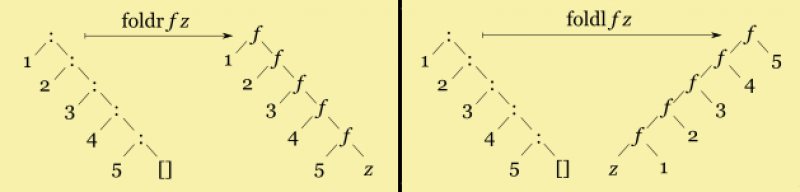
\includegraphics[max width=\textwidth]{:pp:fold-visualization.png}
\end{figure}
:


Tipurile acestor funcții sunt:


\begin{tcblisting}{ arc=0pt, outer arc=0pt, listing only, breakable}
Prelude> :t foldr
foldr :: (a -> b -> b) -> b -> [a] -> b
Prelude> :t foldl
foldl :: (a -> b -> a) -> a -> [b] -> a

\end{tcblisting}


\begin{tcolorbox}[colback=cyan!5, colframe=cyan!10, breakable]
Nu trebie să rețineți pe de rost tipurile. Încercați să înțelegeți ce exprimă și de ce sunt așa.
\end{tcolorbox}

Alte funcții de ordin superior des întâlnite: \texttt{map}, \texttt{filter}, \texttt{zipWith}, \texttt{flip}.


\subsection*{ Exerciții }

1. Fie două matrici reprezentate ca liste de liste. În rezolvarea exercițiilor de mai jos, puteți folosi doar funcții de ordin superior (împreună cu \texttt{take} și \texttt{drop}).

Implementați funcții care să returneze:

\begin{itemize}
	\item  linia \texttt{i} dintr-o matrice
	\item  elementul \texttt{(i, j)} dintr-o matrice
	\item  suma a două matrici
	\item  transpusa unei matrici 
	\item  produsul a două matrici
\end{itemize}


2. O imagine poate fi reprezentată ca o matrice de caractere (numiți, în continuare, "pixeli"). Considerăm că avem trei tipuri de pixeli: \texttt{'.'}, \texttt{'*'}, \texttt{' '}

Implementați următoarele funcții:
\begin{itemize}
	\item  flip orizontal, flip vertical, rotație de 90 în sens trigonometric și invers trigonometric
	\item  negativul (\texttt{'*'} si \texttt{'.'} devin \texttt{' '}, iar \texttt{' '} devine \texttt{'*'})
	\item  scalarea unei imagini cu \texttt{x} unități
	\item  alipirea a două imagini (cu aceeași înălțime) pe orizontală
	\item  alipirea a două imagini (cu aceeași lungime) pe verticală
	\item  crop orizontal de la de la coloana \texttt{x} la coloana \texttt{y}
	\item  crop vertical de la linia \texttt{x} la linia \texttt{y}
	\item  Implementați suprapunerea unei imagini peste o alta (având aceeași dimensiune)
\end{itemize}


\subsection*{ Resurse }

Puteți folosi următoarele pentru a vă testa funcțiile:


\begin{tcblisting}{ arc=0pt, outer arc=0pt, listing only, breakable}
l0="        ***** **            ***** **    "
l1="     ******  ****        ******  ****   "
l2="    **   *  *  ***      **   *  *  ***  "
l3="   *    *  *    ***    *    *  *    *** "
l4="       *  *      **        *  *      ** "
l5="      ** **      **       ** **      ** "
l6="      ** **      **       ** **      ** "
l7="    **** **      *      **** **      *  "
l8="   * *** **     *      * *** **     *   "
l9="      ** *******          ** *******    "
l10="      ** ******           ** ******     "
l11="      ** **               ** **         "
l12="      ** **               ** **         "
l13="      ** **               ** **         "
l14=" **   ** **          **   ** **         "
l15="***   *  *          ***   *  *          "
l16=" ***    *            ***    *           "
l17="  ******              ******            "
l18="    ***                 ***             "

img = [l0,l1,l2,l3,l4,l5,l6,l7,l8,l9,l10,l11,l12,l13,l14,l15,l16,l17,l18]

m1 = [[1, 2, 3], [4, 5, 6], [7, 8, 9]]
m2 = [[1, 0, 0], [0, 1, 1], [1, 0, 1]]

summ1m2 = [[2,2,3],[4,6,7],[8,8,10]]
prodm1m2 = [[4,2,5],[10,5,11],[16,8,17]]

-- functii care printeaza intr-un mod human-readable o matrice sau o imagine
display :: (Show a) => ([a] -> String) -> [[a]] -> IO ()
display displayLine = putStr . foldr (++) "" . map displayLine

-- folositi pentru a afisa o matrice de numere (ex. 1)
displayMat :: (Show a) => [[a]] -> IO ()
displayMat = display (foldr (\x acc -> show x ++ "   " ++ acc) "\n")

-- folositi pentru a afisa o "imagine" - matrice de siruri (ex. 2)
displayImg :: [String] -> IO ()
displayImg = display (++ "\n")


\end{tcblisting}

\section{ Course: Types in functional programming}
\section*{ Types in functional programming }

\subsection*{ Typing in programming languages }

\subsubsection*{ Strong vs weak typing }

Consider the following example from Javascript, where the operator \texttt{+} is applied on arguments of different types. The result is given below:

\begin{tcblisting}{ arc=0pt, outer arc=0pt, listing only, breakable}
[] + []  =  ""  
[] + {}  = "[object]"
{} + []  = 0
{} + {}  = null

\end{tcblisting}
 

where \texttt{[]} is the empty array and \texttt{\{\}} is the empty object. The result is quite surprising, and unpredictable. To explain it, we need to look at the implementation of the Javascript interpreter. In Javascript, there is a distinction between \textbf{primitive} and \textbf{non-primitive} values. Arrays (like \texttt{[]}) and objects (like \texttt{\{\}}) are considered non-primitive. Since the operation \texttt{+} is performed on primitive values, Javascript attempts to \textbf{convert} the operands to primitive. A pseudocode for this is shown below:

\begin{tcblisting}{ arc=0pt, outer arc=0pt, listing only, breakable}
     Convert(value) {
        if (value.valueOf() is a primitive) return it          //conversion to integer works?
        else if (value.toString() is a primitive) return it    //else convert to string, if possible 
             else error
     }

\end{tcblisting}


The conversion of \texttt{[]} to string yields the empty string, while the conversion of \texttt{\{\}} to string yields "[object]". This explains the first two results.

For the latter, we must know that \texttt{\{\}} can also be interpreted as a code-block, and this is the case here. Hence, the Javascript interpreter sees:

\begin{tcblisting}{ arc=0pt, outer arc=0pt, listing only, breakable} 
+ []
+ {}

\end{tcblisting}


where \texttt{+} is interpreted as a \textbf{unary} operator. JavaScript has such an implementation overloading for \texttt{+}. Without going into more details, \texttt{+ x} behaves like a \textit{conversion to Number} for x. Thus, \texttt{[]} converted to \texttt{Number} is \texttt{0}, while \texttt{\{\}} converted to \texttt{Number} is \texttt{NaN} (not a number).

\paragraph{ Morale }\hfill\\

The Javascript treatment of \texttt{+} is unimportant by itself, and it has some advantages for the programmer (although our example shows otherwise). However, we can note that, by allowing any \textbf{kind/type} of operand for \texttt{+}:
\begin{itemize}
	\item  \textbf{complicates the semantics} of the language (the programmer needs to known about conversion to primitives and conversion to numbers)
	\item  \textbf{reduces errors} (no Javascript error was signalled above), but \textbf{makes programs more prone to bugs}.
	\item  makes a program \textbf{more expressive} (\texttt{+} can be used in several ways) but sometimes difficult to use.
\end{itemize}


In programming language design, there is a fundamental tension between \textbf{expressiveness} and \textbf{typing}. Typing is a means for \textbf{enforcing constraints on what is deemed as a \textit{correct program}}. It may be the case that, \textit{conceptually correct} programs may not be accepted as \textbf{correct} from a typing perspective (this situation does seldom occur in Haskell).

A \textbf{strongly-typed} programming language, is more coercive with respect to \textbf{typing constraints}. In functional programming:
\begin{itemize}
	\item  Haskell
	\item  Scala
\end{itemize}
are considered \textbf{strongly-typed}. In imperative / OOP programming, the languages:
\begin{itemize}
	\item  Java
	\item  C++
	\item  Scala
\end{itemize}
are considered \textbf{strongly-typed}.

A \textbf{weakly-typed} programming language is more relaxed w.r.t. \textbf{typing constraints}. For instance, in functional programming:
\begin{itemize}
	\item  Racket (Lisp)
	\item  Clojure
\end{itemize}
are considered \textbf{weakly-typed}. In imperative / OOP programming, the languages:
\begin{itemize}
	\item  C
	\item  Python
	\item  PHP
	\item  Javascript
\end{itemize}

(and especially the latter) are considered weakly-typed. In the latter languages, types are usually reduced to primitive constructs (programmers cannot create new types), or the type construction procedure is very simplistic. For instance, in \texttt{Racket} (formerly known as \texttt{Scheme}), which weakly-typed:
\begin{itemize}
	\item  lists can hold any values (e.g.) \texttt{'(1 \#t "String")}, which means that the type for lists is \textbf{primitive} (not composed), and is simply \texttt{list}.
	\item  functions can return values of different types - the type for functions is also \textbf{primitive} - \texttt{\#procedure}. 
\end{itemize}

However, type verification is not absent in weakly-typed languages, including Racket/Scheme. For instance, the call \texttt{(+ 1 '())} will produce an error since the plus operator is called on values with invalid types.

We shall discuss Scheme/Racket in more detail later. It is worth noting that, in Racket there exists extensions (Typed Racket) which allow programmers to define and compose types to some extent.

The \textbf{weakly-typed} vs \textbf{strongly-typed} classification is not rigid and is subject to debate and discussion. There is no objective \textit{right-answer}. For instance, here, the language \texttt{C} is viewed as weakly-typed. We illustrate a small motivating example:


\begin{tcblisting}{ arc=0pt, outer arc=0pt, listing only, breakable}
int f (int x) {
    if (x != 0)
        return 1;
    return malloc(100);
}

\end{tcblisting}


In principle, the function \texttt{f} can return an integer, or a pointer to any object (of any type), and this is allowed by the compiler (which does issue a warning). Compared to, e.g. Java, this makes the \texttt{C} type system more relaxed.

There are valid arguments for considering \texttt{C} as strongly-typed and, as said before, there is no right answer.

\subsubsection*{ Compile-time vs runtime typing }

This classification is done w.r.t. \textbf{the moment} when type inference occurs:
\begin{itemize}
	\item  during the \textbf{compilation} of a program
	\item  at \textbf{runtime}
\end{itemize}

The former is also called \textbf{static typing}, while the latter - \textbf{dynamic typing}. In the literature, \textbf{static} and \textbf{dynamic} typing are also used with other meanings, hence, here, we prefer the terms \textbf{compile-time} and \textbf{runtime}.

The imperative/OOP languages:
\begin{itemize}
	\item  Java
	\item  Scala
	\item  C\textbackslash C++
\end{itemize}

perform compile-time type checking, as well as the functional languages:
\begin{itemize}
	\item  Haskell 
	\item  Scala
\end{itemize}

The imperative/OOP languages:
\begin{itemize}
	\item  Python
	\item  PHP
	\item  Javascript
\end{itemize}

perform runtime type checking, as well as the functional languages:
\begin{itemize}
	\item  Scheme/Racket (Lisp)
	\item  Clojure
\end{itemize}

Compile-time type checking is preferred for strongly-typed languages: the complexity of type verification is delegated to the compiler. Conversely, in weakly-typed languages, type verification is simpler, hence it can be performed by the interpreter, at runtime. Sometimes, a compiler may be absent. This is not a golden rule but merely an observation.

While runtime type checking is simpler to deploy, it has the disadvantage of not capturing typing bugs. Consider the following program in Racket:

\begin{tcblisting}{ arc=0pt, outer arc=0pt, listing only, breakable}
(define f (lambda (x) (if x 1 (+ 1 '()))))
(f #t)

\end{tcblisting}


The function receives a value \texttt{x} which must be a boolean. In the program above there is no error, even though \texttt{(+ 1 '())} is an incorrectly-typed function call. However, in the execution of the program (i.e. \texttt{(f \#t)}), the else branch of the function is not reached, hence no typing verification is performed.

Hence, runtime type checking only catches bugs \textbf{on the current program execution trace}.


\subsection*{ Typing in Haskell }

\subsection*{ Type inference in Haskell }

Haskell implements the \texttt{ Hindley-Milner type inference algorithm} \footnote{\url{https://en.wikipedia.org/wiki/Hindley\%E2\%80\%93Milner\_type\_system }}. In what follows, we present a simplified, and more easy-to-follow, but incomplete algorithm which serves as an illustration for the main concepts underlying the original one. 

\subsubsection*{ Intro }

Consider the following expressions, and their types:

\begin{tcblisting}{ arc=0pt, outer arc=0pt, listing only, breakable}
\x -> x + 1 :: Integer -> Integer
\x -> if x then 0 else 1 :: Bool -> Integer
zipWith (:) :: [a] -> [[a]] -> [[a]]
\f -> (f 1) + (f 2) :: (Integer -> Integer) -> Integer

\end{tcblisting}


We can see via the above example that types are constructed according to the following grammar:


\begin{tcblisting}{ arc=0pt, outer arc=0pt, listing only, breakable}
type ::= <const_type> | <type_var> | (<type>) | type -> type | [<type>]

\end{tcblisting}


This grammar only tells half the story regarding Haskell typing, however, for the purposes of this lecture, this view suffices. According to the above grammar, types can be:
\begin{itemize}
	\item  \textbf{constant types} (e.g. \texttt{Integer}, \texttt{String})
	\item  \textbf{type variables} (e.g. \texttt{a} - which are usually used to designate \textbf{any} possible type, as in \texttt{[a]})
	\item  \textbf{function types} (e.g. \texttt{Integer -\textgreater  Integer} or \texttt{(Integer -\textgreater  Integer)} if this type appears in a larger type expression)
	\item  \textbf{list types} (e.g. \texttt{[a]}).
	\item  any combination of the above rules.
\end{itemize}


\subsubsection*{ Expression trees }

We assume each Haskell expression is constructed via the following \textit{construction rules}:
\begin{itemize}
	\item  \textbf{functional application} (e.g. \texttt{take 2 [1,2,3]})
	\item  \textbf{function definition} (e.g. \texttt{\textbackslash x-\textgreater [x+1]})
\end{itemize}

We note that many Haskell definitions can be seen as such. For instance:

\begin{tcblisting}{ arc=0pt, outer arc=0pt, listing only, breakable}
g f = (f 1) + 1
<code>

can be seen as:

<code haskell>
g = \f -> (f 1) + 1

\end{tcblisting}


Hence, we can take any Haskell expression, and construct a \textbf{tree}, in which each node represents a \textbf{construction rule}, and children represent sub-expressions:
\begin{itemize}
	\item  for functional applications, the children are the \textbf{function name} and \textbf{the parameters}
	\item  for function definition, the children are \textbf{the variable/variables} and the \textbf{function body}.
\end{itemize}

For example, consider the expression tree for the function \texttt{g} shown previously (we use tabs to illustrate parent/child relationship):

\begin{tcblisting}{ arc=0pt, outer arc=0pt, listing only, breakable}
\f -> (f 1) + 1
  f
  (f 1) + 1
    (+)
    (f 1)
       f 
       1
    1

\end{tcblisting}


In what follows, we shall use expression trees to perform type inference.

\subsubsection*{ Typing rules }

We introduce the following \textbf{typing rules}:

\paragraph{ Rule (TVar) }\hfill\\

If \texttt{v} is bound to a constant expression e of type \texttt{ct}, then \texttt{v :: ct}

\paragraph{ Rule (TFun) }\hfill\\

If \texttt{x :: t1} and \texttt{e :: t2} then \texttt{\textbackslash x -\textgreater  e  :: t1 -\textgreater  t2}

\paragraph{ Rule (TApp) }\hfill\\

If \texttt{f :: t1 -\textgreater  t2} and \texttt{e :: t1} then \texttt{(f e) :: t2}

The above rule can be naturally generalised:

If \texttt{f :: t1 -\textgreater  t2 -\textgreater  ... -\textgreater  tn -\textgreater  t} and \texttt{e1 :: t1}, ..., \texttt{en :: tn} then \texttt{(f e1 ... en) :: t}

In what follows, we will use these rules to make judgements on our types. These rules have a twofold usage:
\begin{itemize}
	\item  \textbf{deduce} the type of an expression, based on \textit{existing knowledge}
	\item  \textbf{make hypotheses} regarding the type of an expression (we shall not focus on this aspect in the presentation))
\end{itemize}

\subsubsection*{ Type inference stage 1: Expression tree construction }

Type inference for an expression \texttt{e} can be seen as having two stages. In the first stage, we:
\begin{itemize}
	\item  construct the expression tree of \texttt{e}
	\item  make \textbf{hypotheses} regarding the types of \textbf{yet untyped} expressions (e.g. variables).
\end{itemize}

We illustrate the first stage on the previous definition of \texttt{g}:


\begin{tcblisting}{ arc=0pt, outer arc=0pt, listing only, breakable}
\f -> (f 1) + 1 :: ?
  f :: tf (here we introduce tf as the type of f. This is a type hypothesis)
  (f 1) + 1 :: ?
    (+) :: ?
    (f 1) :: ?
       f :: t1 -> t2 (this is another hypothesis, stemming from the fact that f is applied on 1)
       1 :: ?
    1 :: ?

\end{tcblisting}


\subsubsection*{ Type inference stage 2: Rule application }

In this stage, we start from the previously-build tree, and:
\begin{itemize}
	\item  \textbf{apply typing rules} to deduce types for new sub-expressions
	\item  \textbf{perform type unification}: This is one aspect that we shall not elaborate on, in this lecture. 
\end{itemize}

This is equivalent to a \textbf{bottom-up} tree traversal: We start from the leaves, and progress to the root (i.e. the expression to be typed).

Without delving into details, \textbf{type unification} is an important ingredient, because it allows us to infer \textbf{the most general} type of an expression. Consider the following Haskell expression: \texttt{\textbackslash f x -\textgreater  (f x,f 1)}, which defines a function that takes another function \texttt{f}, a value \texttt{x} and returns a pair: the first element of the pair is the application \texttt{f x}, while the second - \texttt{f 1}:
\begin{itemize}
	\item  initially, we do not know what \texttt{f} is, hence it has \textbf{the most general type} (say) \texttt{tf} - it can be anything;
	\item  judging by the application \texttt{f x}, we deduce that \texttt{f} must be a function, of type \texttt{a-\textgreater b}, where \texttt{x::a}
	\item  judging by the application \texttt{f 1}, we deduce that \texttt{a} must be an \texttt{Integer}
\end{itemize}
The unification process combines the information collected so far:
\begin{itemize}
	\item  \texttt{tf} must unify (coincide with) \texttt{a -\textgreater  b}
	\item  \texttt{a} must unify with \texttt{Integer}
\end{itemize}

The final type for the expression is: \texttt{(Integer -\textgreater  b) -\textgreater  Integer -\textgreater  (b, b)}

We illustrate the second stage of the type inference on the same example:


\begin{tcblisting}{ arc=0pt, outer arc=0pt, listing only, breakable}
\f -> (f 1) + 1 :: tf -> Integer
  f :: tf (via (TFun))
  (f 1) + 1 :: Integer (via (TApp))
    (+) :: Integer -> Integer -> Integer (this we know from Prelude, after the type synthesis of (+), also t2 must unify with Integer)
    (f 1) :: t2 (via (TApp); also, t1 must unify with Integer)
       f :: t1 -> t2
       1 :: Integer (via (TVar), from Prelude)
    1 :: Integer (via (TVar), from Prelude)

\end{tcblisting}


The (pseudo)-algorithmic procedure concludes with the following answer:
\begin{itemize}
	\item  \texttt{g :: tf -\textgreater  Integer}, where

  \begin{itemize}
  	\item  \texttt{tf} unifies with \texttt{t1 -\textgreater  t2}
  	\item  \texttt{t2} unifies with \texttt{Integer}
  	\item  \texttt{t1} unifies with \texttt{Integer}
  \end{itemize}
\end{itemize}

After unification, the result is shown to the programmer: \texttt{ g :: (Integer -\textgreater  Integer) -\textgreater  Integer}

Exercises. Find the type of the following expressions, by applying the type synthesis pseudo-algorithm:
\begin{itemize}
	\item  \texttt{map (\textbackslash x-\textgreater [x+1])}
	\item  \texttt{\textbackslash f x-\textgreater  if x then f x else x}
	\item  \texttt{g f x = x \&\& (f x)}
	\item  \texttt{g f = f (g f)}
\end{itemize}


\section{ Course: Abstract datatypes}
\subsection*{ Abstract Datatypes }

\subsubsection*{ Intro }

An Abstract Datatype relies on \textit{functions} to describe the possible values of a type. We start with a simplistic example:


\begin{tcblisting}{ arc=0pt, outer arc=0pt, listing only, breakable}
data Nat = Zero | Succ Nat

\end{tcblisting}

\begin{itemize}
	\item  the expression \texttt{data Nat} introduces a new \textbf{type} in the programming language
	\item  after \texttt{=}, the \textbf{base constructors} of the type follow. In Haskell, \textbf{all constructors} must begin with a capital letter
	\item  \texttt{Zero} is a nullary constructor. 
	\item  \texttt{Succ Nat} designates an \textbf{internal} constructor, which expects a natural number (of type \texttt{Nat}). A value \texttt{(Succ x)} \textbf{is} of type \texttt{Nat} (i.e. a natural number), and we may be tempted to see it as a function call, which \textit{returns} the successor of \texttt{x}
\end{itemize}

\texttt{Zero} and \texttt{Succ} are called \textbf{data constructors} in Haskell. \texttt{Nat} is called a \texttt{type} or \texttt{type-constructor}. We shall distinguish between the two in a later lecture.

Note that the \textit{internal} representation of an ADT, as perceived by the programmer, is \textit{abstract}. We may see values as \textit{calls} of special functions - data constructors. Except for their meaning (and language-level implementation), data constructors behave exactly as functions. For instance:
\begin{itemize}
	\item  \texttt{Zero :: Nat}
	\item  \texttt{Succ :: Nat -\textgreater  Nat}
\end{itemize}

We continue the example with addition:


\begin{tcblisting}{ arc=0pt, outer arc=0pt, listing only, breakable}
add :: Nat -> Nat -> Nat
add Zero y = y
add (Succ x) y = Succ (add x y)

\end{tcblisting}


An important observation is that the \textbf{pattern matching mechanism} in Haskell relies on data constructors, and their applications. For instance, the following definition is a correct usage of the pattern matching mechanism:

\begin{tcblisting}{ arc=0pt, outer arc=0pt, listing only, breakable}
f (1:y:[]) = ...

\end{tcblisting}

I uses the data constructors \texttt{(:)} and \texttt{[]} for lists, as well as the data constructor \texttt{1} for integers. The pattern describes any list of integers which starts with a \texttt{1} and contains exactly two elements.

\subsubsection*{ Monomorphic List implementation }

In what follows, we give an implementation for the type \textit{List of integers}. This type is called \textit{monomorphic}, since our list can only contain elements of a single type (integer):


\begin{tcblisting}{ arc=0pt, outer arc=0pt, listing only, breakable}
data IList = Void | Cons Integer IList

app :: IList -> IList -> IList
app Void l = l
app (Cons h t) l = Cons h (app t l)

convert :: IList -> [Integer]
convert Void = []
convert (Cons h t) = h : (convert t)

mfoldl :: (b -> Integer -> b) -> b -> IList -> b
mfoldl op acc Void = acc
mfoldl op acc (Cons h t) = mfoldl op (op acc h) t

mfoldr :: (Integer -> a -> a) -> a -> IList -> a
mfoldr op acc Void = acc
mfoldr op acc (Cons h t) = op h (mfoldr op acc t)

convert2 :: IList -> [Integer]
convert2 = mfoldr (:) []

showl :: IList -> String
showl = show . convert2


\end{tcblisting}


In the above code, we have defined some basic list operations, such as \texttt{app} (list concatenation) and \texttt{convert}, which transforms a list of type \texttt{IList} to a conventional Haskell list (of type \texttt{[Integer]}).

We have also implemented the two folding procedures for \texttt{IList}. Note the type signature of each fold. Finally, we have used folds to provide an alternative implementation for convert, as well as for converting lists to strings.


\subsubsection*{ Propositional Logic in Haskell }

Abstract Datatypes are a natural way to define more elaborate data-structures, such as propositional formulae. We give a possible definition below:


\begin{tcblisting}{ arc=0pt, outer arc=0pt, listing only, breakable}
data Formula = Var String | And Formula Formula | Or Formula Formula | Not Formula

\end{tcblisting}


We observe that:
\begin{itemize}
	\item  \texttt{Var :: String -\textgreater  Formula}
	\item  \texttt{And :: Formula -\textgreater  Formula -\textgreater  Formula}
	\item  \texttt{Or :: Formula -\textgreater  Formula -\textgreater  Formula}
	\item  \texttt{Not :: Formula -\textgreater  Formula}
\end{itemize}

A good exercise consists in the implementation of a display function for formulae:

\begin{tcblisting}{ arc=0pt, outer arc=0pt, listing only, breakable}
fshow :: Formula -> String
fshow (Var v) = v
fshow (And f1 f2) = "("++(fshow f1)++" ^ "++(fshow f2)++")"
fshow (Or f1 f2) = "("++(fshow f1)++" V "++(fshow f2)++")"
fshow (Not f) = "~("++(fshow f)++")"

\end{tcblisting}


Next, we implement a function \texttt{push}, which pushes negation \textit{inward}:

\begin{tcblisting}{ arc=0pt, outer arc=0pt, listing only, breakable}
push :: Formula -> Formula
push (Var v) = (Var v)
push (Not (Var v)) = Not (Var v)
push (Not (And f1 f2)) = Or (push (Not f1)) (push (Not f2))
push (Not (Or f1 f2)) = And (push (Not f1)) (push (Not f2))
push (And f1 f2) = And (push f1) (push f2)
push (Or f1 f2) = Or (push f1) (push f2)

\end{tcblisting}


Notice, at lines 4,5 the implementation of deMorgan's laws.

Finally, we implement a function which computes the truth-value of a formula, under a certain interpretation. First, we define the type \texttt{Interpretation}:

\begin{tcblisting}{ arc=0pt, outer arc=0pt, listing only, breakable}
type Interpretation = String -> Bool

i :: Interpretation
i "x" = True
i "y" = False
i "z" = True

\end{tcblisting}
 

In the first line, we have defined a \textbf{type-alias}: \texttt{Interpretation} is a function from strings to booleans. We have also implemented a three-variable interpretation, for testing purposes. Next, we implement \texttt{eval}:


\begin{tcblisting}{ arc=0pt, outer arc=0pt, listing only, breakable}
eval :: Interpretation -> Formula -> Bool
eval i (Var v) = i v
eval i (Not f) = not(eval i f)
eval i (And f1 f2) = (eval i f1) &\&&&\&& (eval i f2)
eval i (Or f1 f2) = (eval i f1) || (eval i f2)

\end{tcblisting}


\subsubsection*{ Monomorphic Trees in Haskell }


\begin{tcblisting}{ arc=0pt, outer arc=0pt, listing only, breakable}
data ITree = Leaf | Node ITree Integer ITree

\end{tcblisting}


Note that:
\begin{itemize}
	\item  \texttt{Leaf :: ITree}
	\item  \texttt{Node :: ITree -\textgreater  Integer -\textgreater  ITree -\textgreater  ITree}
\end{itemize}

Next, we implement a folding operation on Trees. The key to it is to conceptually define what folding should do on Trees. To grasp an intuition, recall that: 
\begin{itemize}
	\item  \texttt{foldr (:) []} is the \textbf{identity function} on lists. Hence, \texttt{foldr (:) [] [1,2,3]} produces \texttt{[1,2,3]}.
	\item  also, recall that the map operation can be defined as: \texttt{\textbackslash f -\textgreater  foldr ((:).f) []}
\end{itemize}

Similar to the list case, a fold on trees should:
\begin{itemize}
	\item  \textbf{preserve the tree structure}, given the appropriate operator (e.g. \texttt{Node}). 
	\item  hence, the call \texttt{mtfold Node Leaf} (where \texttt{Leaf} is the accumulator) should be the \textbf{identity function on trees}. 
\end{itemize}

Let us define the identity function \texttt{tid} for trees:

\begin{tcblisting}{ arc=0pt, outer arc=0pt, listing only, breakable}
tid Leaf = Leaf
tid (Node r k l) = Node (tid r) k (tid l)

\end{tcblisting}


As already said, \texttt{(tid t)} is equivalent to the call \texttt{(mtfold Node Leaf t)}, for any arbitrary tree \texttt{t}.
To obtain the general \texttt{mtfold} implementation, we simply generalise \texttt{Node} by an arbitrary operation \texttt{op}:
\begin{itemize}
	\item  if \texttt{Node :: ITree -\textgreater  Integer -\textgreater  ITree -\textgreater  ITree}, then
	\item  \texttt{op :: b -\textgreater  Integer -\textgreater  b -\textgreater  b}
\end{itemize}

We also generalise \texttt{Leaf} by an arbitrary accumulator:
\begin{itemize}
	\item  if \texttt{Leaf :: ITree} then
	\item  \texttt{acc :: b}
\end{itemize}

The code generalisation becomes:


\begin{tcblisting}{ arc=0pt, outer arc=0pt, listing only, breakable}
mtfold :: (b -> Integer -> b -> b) -> b -> ITree -> b
mtfold op acc = 
    let f (Node left key right) = f (f left) key (f right)
        f Leaf = acc
    in f

\end{tcblisting}


Notice that \texttt{f} is precisely the generalisation of \texttt{tid} according to our observations. We can use \texttt{mtfold} to implement various tree operations such as:


\begin{tcblisting}{ arc=0pt, outer arc=0pt, listing only, breakable}
tsum = mtfold (\k r l->k + r + l) 0 
tmirror = mtfold (\k r l -> Node l k r) Leaf 
tflatten = mtfold (\k r l -> r ++ [k] ++ l) [] 

\end{tcblisting}
 
\subsection{ Lab: Abstract datatypes}
\section*{ Tipuri de date abstracte }

Scopul laboratorului:
\begin{itemize}
	\item  Recapitularea conceptului de TDA
	\item  Definirea de TDA-uri în Haskell
	\item  Familiarizarea cu conceptul de TDA-uri polimorfice
	\item  Introducerea tipului de date \texttt{Maybe}
\end{itemize}


\subsection*{ Tipuri de date abstracte (TDA) }

\textbf{Tipurile de date abstracte} sunt modele pentru a defini tipuri de date în funcție de comportamentul acestora (valori posibile, axiome, operații), contrastând cu \textit{structurile de date}, definite din punct de vedere al implementării.

Un TDA familiar este \textbf{list}. \\Pentru a lucra cu liste într-un limbaj ca Java, am scris două \textit{implementări} distincte, și anume \texttt{LinkedList} și \texttt{ArrayList}. Ambele implementări respectă specificațiile din primul paragraf.

\begin{tcolorbox}[colback=yellow!40, colframe=yellow!60, breakable]
Unii autori includ în descrierea TDA-urilor și complexități. Din acest punct de vedere, implementările 
\texttt{LinkedList} și \texttt{ArrayList} diferă.
\end{tcolorbox}


\subsubsection*{ Constructori }

Valorile posibile ale unui TDA sunt date de constructorii acestuia.\\Să considerăm un tip simplu de date: \texttt{Bool}, care poate avea două valori: \texttt{False} și \texttt{True}.\\Sintaxa Haskell pentru a defini acest tip de date este următoarea:


\begin{tcblisting}{ arc=0pt, outer arc=0pt, listing only, breakable}
data Bool = False | True

\end{tcblisting}


\begin{tcolorbox}[colback=yellow!40, colframe=yellow!60, breakable]
Atât numele tipului de date cât și numele constructorilor trebuie scris cu literă mare.
\end{tcolorbox}

\texttt{False} și \texttt{True} nu sunt parametrizate și pot fi privite ca valori. Se mai numesc și \textit{constructori nulari}.\\
Să considerăm un alt TDA care descrie un arbore binar cu valori întregi. Arborele poate fi gol sau un nod cu doi copii.


\begin{tcblisting}{ arc=0pt, outer arc=0pt, listing only, breakable}
data Tree = Nil | Node Int Tree Tree

\end{tcblisting}


\texttt{Node} este un constructor care primește un argument de tipul \texttt{Int} și două argumente de tip \texttt{Tree}, pentru a creea o valoare de tip \texttt{Tree}. Putem să ne gândim la el ca la o funcție:


\begin{tcblisting}{ arc=0pt, outer arc=0pt, listing only, breakable}
Prelude> :t Node
Node :: Int -> Tree -> Tree -> Tree

\end{tcblisting}


Constructorii sunt foarte importanți în \textit{pattern matching}. Ca exemplu, vom scrie o funcție care însumează toate valorile dintr-un arbore:


\begin{tcblisting}{ arc=0pt, outer arc=0pt, listing only, breakable}
treeSum :: Tree -> Int
treeSum Nil = 0
treeSum (Node v l r) = v + (treeSum l) + (treeSum r)

\end{tcblisting}


Observăm prezența a două pattern-uri: unul pentru arborele vid, celălalt pentru un nod, într-un fel foarte asemănător cu modul în care lucram cu liste, făcând pattern matching pe \texttt{[]} și \texttt{(x:xs)}.

\begin{tcolorbox}[colback=cyan!5, colframe=cyan!10, breakable]
Observați că ghci nu știe cum să afișeze arborele nostru:


\begin{tcblisting}{ arc=0pt, outer arc=0pt, listing only, breakable}
Prelude> Node 1 Nil Nil

<interactive>:38:1:
    No instance for (Show Tree) arising from a use of 'print'
    In a stmt of an interactive GHCi command: print it

\end{tcblisting}


Pentru a vă fi mai ușor să vă verificați, puteți obține o reprezentare a tipurilor definite de voi astfel:


\begin{tcblisting}{ arc=0pt, outer arc=0pt, listing only, breakable}
data Tree = Nil | Node Int Tree Tree deriving (Show)

\end{tcblisting}


Pe scurt, acest lucru înrolează TDA-ul vostru în clasa \texttt{Show}, oferind o implementare implicită a funcției \texttt{show} (apelată de ghci). Mai multe detalii în laboratorul următor.


\begin{tcblisting}{ arc=0pt, outer arc=0pt, listing only, breakable}
Prelude> Node 1 Nil Nil
Node 1 Nil Nil

\end{tcblisting}

\end{tcolorbox}


\subsubsection*{ Înregistrări }

Vrem să definim un TDA pentru a descrie un student, folosind următoarele câmpuri: nume, prenume, an de studiu, medie.


\begin{tcblisting}{ arc=0pt, outer arc=0pt, listing only, breakable}
-- tipul de date si constructorul au acelasi nume, ceea ce este ok
-- pentru ca reprezinta concepte diferite.
data Student = Student String String Int Float

\end{tcblisting}


Observăm că semnficația câmpurilor nu este evidentă din definiție. Vrem să extragem valori dintr-un Student; definim funcțiile:


\begin{tcblisting}{ arc=0pt, outer arc=0pt, listing only, breakable}
nume :: Student -> String
nume (Student n _ _ _) = n

prenume :: Student -> String
prenume (Student _ p _ _) = p

an :: Student -> Int
an (Student _ _ a _) = a

medie :: Student -> Float
medie (Student _ _ _ m) = m

\end{tcblisting}


Pentru a face descrierea tipului de date mai clară și a evita să scriem manual acele funcții, putem folosi sintaxa:


\begin{tcblisting}{ arc=0pt, outer arc=0pt, listing only, breakable}
data Student = Student { nume :: String
                       , prenume :: String
                       , an :: Int
                       , medie :: Float
                       }

\end{tcblisting}

                      


\subsection*{ TDA-uri polimorfice }

Până acum, am definit TDA-uri care lucrează doar cu întregi. Dorim să scăpăm de această limitare și să definim TDA-uri care pot lucra cu orice alt tip de date. De exemplu, are sens să considerăm capul unei liste care conține elemente de tip \texttt{a}, ca fiind un element de tip \texttt{a}, indiferent de cum arată acest tip.\\
Într-adevăr, aceasta este definiția funcției \texttt{head} existentă în Haskell:


\begin{tcblisting}{ arc=0pt, outer arc=0pt, listing only, breakable}
Prelude> :t head
head :: [a] -> a

\end{tcblisting}


\texttt{a} se numește \textbf{variabilă de tip} și poate să reprezinte orice tip de date (evident, cu condiția ca toate \texttt{a}-urile care apar să se refere la același tip).

\begin{tcolorbox}[colback=blue!10, colframe=blue!20]
Să ne uităm la tipul altei funcții cunoscute:


\begin{tcblisting}{ arc=0pt, outer arc=0pt, listing only, breakable}
Prelude> :t map
map :: (a -> b) -> [a] -> [b]

\end{tcblisting}


\texttt{map} primește ca argument o funcție - care primește un element de tip \texttt{a} și întoarce un element de tip \texttt{b} - și o listă de elemente de tip \texttt{a} și întoarce o listă de elemente de tip \texttt{b}. De precizat că \texttt{a} și \texttt{b} pot fi distincte dar nu este necesar.
\end{tcolorbox}

Listele din Haskell sunt \textbf{polimorfice}. Ele pot conține date de orice tip. O instanță a listelor are însă un tip concret:


\begin{tcblisting}{ arc=0pt, outer arc=0pt, listing only, breakable}
Prelude> :t ['a', 'b', 'c']
['a', 'b', 'c'] :: [Char]

\end{tcblisting}


\subsubsection*{ Constante polimorfice }

Care este tipul listei vide?


\begin{tcblisting}{ arc=0pt, outer arc=0pt, listing only, breakable}
Prelude> :t []
[] :: [a]

\end{tcblisting}


Observăm că tipul listei vide este general. Asta înseamnă că lista vidă poate fi tratată ca o listă de orice tip.


\begin{tcblisting}{ arc=0pt, outer arc=0pt, listing only, breakable}
Prelude> [1,2,3] ++ "123" -- eroare, tipuri diferite
Prelude> [1,2,3] ++ []
[1,2,3]
Prelude> "123" ++ []
"123"

\end{tcblisting}


Spunem că \texttt{[]} este o \textbf{constantă polimorfică}.

\begin{tcolorbox}[colback=blue!10, colframe=blue!20]
O altă constantă polimorfică este, de exemplu \texttt{1}. De aceea putem scrie:


\begin{tcblisting}{ arc=0pt, outer arc=0pt, listing only, breakable}
Prelude> 1 + 2
3
Prelude> 1 + 2.71
3.71

\end{tcblisting}


Dacă forțăm 1 să fie întreg, vom primi o eroare la a doua adunare:

\begin{tcblisting}{ arc=0pt, outer arc=0pt, listing only, breakable}
Prelude> (1 :: Int) + 2.71

<interactive>:60:14:
    No instance for (Fractional Int) arising from the literal '2.71'
    In the second argument of '(+)', namely '2.71'
    In the expression: (1 :: Int) + 2.71
    In an equation for 'it': it = (1 :: Int) + 2.71

\end{tcblisting}


\texttt{1} are însă o constrângere despre care vom discuta în laboratorul următor.
\end{tcolorbox}


Pentru a implementa în Haskell un TDA polimorfic, folosim sintaxa:


\begin{tcblisting}{ arc=0pt, outer arc=0pt, listing only, breakable}
data List a = Empty | Cons a (List a)

\end{tcblisting}


\begin{tcolorbox}[colback=blue!10, colframe=blue!20]
Ce este \texttt{List}?\\
\texttt{List} este un \textbf{constructor de tip}, nu un tip de date. Constructorii de tip primesc ca parametrii \textit{tipuri} și întorc un tip (sau un alt constructor de tip dacă nu primesc suficienți parametrii).\\Asta înseamnă că, \texttt{List} nu este un \textit{tip}, dar \texttt{List Int}, \texttt{List Char} etc. sunt tipuri.
\end{tcolorbox}

\subsubsection*{ Maybe și Either }

Unul dintre TDA-urile puse la dispoziție de Haskell este \texttt{Maybe}, un tip \textit{polimorfic} care modelează prezența unei anumite valori, sau absența acesteia:

\begin{tcblisting}{ arc=0pt, outer arc=0pt, listing only, breakable}
data Maybe a = Nothing | Just a

\end{tcblisting}


Pentru a ilustra importanța acestui TDA, considerăm următoare situație: vrem să implementăm o funcție care returnează suma valoriilor celor doi copii ai unui nod dat:


\begin{tcblisting}{ arc=0pt, outer arc=0pt, listing only, breakable}
childrenSum :: Tree -> Maybe Int
childrenSum Nil = Nothing
childrenSum (Node _ Nil _) = Nothing
childrenSum (Node _ _ Nil) = Nothing
childrenSum (Node _ (Node v _ _) (Node w _ _)) = Just (v + w)

\end{tcblisting}


Această sumă există doar pentru arbore diferit de Nil, cu ambii copii diferiți de Nil.

Putem scrie o funcție care ia un \texttt{Maybe} și returnează un șir pentru printare. Combinăm apoi cele două funcții:


\begin{tcblisting}{ arc=0pt, outer arc=0pt, listing only, breakable}
pretty :: Maybe Int -> String
pretty Nothing = "No value"
pretty (Just v) = "Sum is " ++ show v

printChildrenSum :: Tree -> String
printChildrenSum = pretty . childrenSum

\end{tcblisting}


Încărcăm modulele în ghci și voilà:

\begin{tcblisting}{ arc=0pt, outer arc=0pt, listing only, breakable}
*Main> printChildrenSum (Node 1 (Node 1 Nil (Node 2 Nil Nil)) (Node 3 (Node 4 (Node 5 Nil Nil) Nil) (Node 6 Nil Nil)))
"Sum is 4"
*Main> printChildrenSum Nil
"No value"
*Main> printChildrenSum (Node 1 Nil (Node 1 Nil Nil))
"No value"
*Main> printChildrenSum (Node 1 (Node 1 Nil Nil) Nil)
"No value"

\end{tcblisting}


Un TDA similar este \texttt{Either}, care modelează valori cu două tipuri posibile:


\begin{tcblisting}{ arc=0pt, outer arc=0pt, listing only, breakable}
data Either a b = Left a | Right b

\end{tcblisting}


Prin convenție, constructorul \texttt{Left} reprezintă o eroare, iar constructorul \texttt{Right} o valoare corectă. Astfel putem extinde mecanisme de error-handling pentru a conține mai multe informații despre ce a cauzat eroarea (spre deosebire de \texttt{Maybe}, care doar indică \textbf{existența} unei erori):


\begin{tcblisting}{ arc=0pt, outer arc=0pt, listing only, breakable}
childrenSum :: Tree -> Either String Int
childrenSum Nil = Left "Tree is Nil"
childrenSum (Node _ Nil _) = Left "Left child is Nil"
childrenSum (Node _ _ Nil) = Left "Right child is Nil"
childrenSum (Node _ (Node v _ _) (Node w _ _)) = Right (v + w)

pretty :: Either String Int -> String
pretty (Left s) = s
pretty (Right i) = "Sum is " ++ show i

printChildrenSum :: Tree -> String
printChildrenSum = pretty . childrenSum

\end{tcblisting}



\begin{tcblisting}{ arc=0pt, outer arc=0pt, listing only, breakable}
*Main> printChildrenSum (Node 1 (Node 1 Nil (Node 2 Nil Nil)) (Node 3 (Node 4 (Node 5 Nil Nil) Nil) (Node 6 Nil Nil)))
"Sum is 4"
*Main> printChildrenSum Nil
"Tree is Nil"
*Main> printChildrenSum (Node 1 Nil (Node 1 Nil Nil))
"Left child is Nil"
*Main> printChildrenSum (Node 1 (Node 1 Nil Nil) Nil)
"Right child is Nil"

\end{tcblisting}


\subsubsection*{ Exerciții }

\begin{tcolorbox}[colback=yellow!40, colframe=yellow!60, breakable]
Încercați să vă obișnuiți să scrieți explicit tipurile tuturor funcțiilor definite de voi în continuare.
\end{tcolorbox}

\subparagraph{ 1. List }\hfill\\

a) implementați TDA-ul pentru propria voastră listă care poate conține doar numere întregi\\b) scrieți o funcție care convertește valori ale TDA-ului vostru în liste din Haskell

\begin{tcolorbox}[colback=cyan!5, colframe=cyan!10, breakable]
Dacă tipul vostru de listă se numește \texttt{List}, atunci tipul funcției va fi: 


\begin{tcblisting}{ arc=0pt, outer arc=0pt, listing only, breakable}
convertList :: List -> [Int]

\end{tcblisting}

\end{tcolorbox}

c) modificați tipul \texttt{List} pentru a fi polimorfic, apoi modificați și funcția \texttt{convertList}

\subparagraph{ 2. Tree }\hfill\\
a) Implementați TDA-ul pentru arbori polimorfici.\\b) Implementați \texttt{foldT}, echivalentul lui \texttt{foldr} (puteți vizualiza rezultatul ca fiind înlocuirea tuturor constructorilor nulari cu o valoare constantă și a tuturor celorlalți constructori cu funcții care iau același numă de argumente.\\c) Implementați o funcție \texttt{mapT} (echivalentul lui \texttt{map}), folosindu-vă de \texttt{foldT}.\\d) Implementați o funcție \texttt{zipWithT} (echivalentul lui \texttt{zipWith}).\\
\subparagraph{ 3. Numere naturale extinse }\hfill\\
a) Implementați un TDA care să modeleze numere naturale extinse cu un punct la infinit ($ \hat{\mathbb{N}} = \mathbb{N} \cup \{ \infty \}$).\\b) Implementați o funcție \texttt{extSum} care să evalueze suma a două numere naturale extinse.\\c) Implementați o funcție \texttt{extDiv} care să evalueze raportul a două numere naturale extinse (împărțirea la 0 și la infinit are rezultat definit).\\d) Implementați o funcție \texttt{extLess} care spune dacă un număr natural extins e mai mic decât un altul.

În laboratorul următor, vom vedea cum putem implementa aceste operații într-un mod consistent cu restul limbajului, folosind operatori cunoscuți (\texttt{+}, \texttt{div}, \texttt{\textless }).
                   
\subparagraph{ 4. Înregistrări }\hfill\\

a) Scrieți un TDA care codifică un tuplu (înregistrare) format din următoarele câmpuri:
   \begin{itemize}
   	\item  Nume (codificat ca String)
   	\item  Vârstă (codificat ca Integer)
   	\item  Prieteni (codificat ca o lista de String-uri)
   	\item  Notă PP (codificat ca Integer). Acest câmp este opțional!
   \end{itemize}

b) Scrieți o funcție care primește o listă de înregistrări și le întoarce pe acelea pentru care vârsta este mai mare ca 20.\\c) Scrieți o funcție care primește o listă de înregistrări și le întoarce pe acelea care conțin cel puțin un prieten cu numele "Matei".\\d) Scrieți o funcție care primește o listă de înregistrări și le întoarce pe acelea care conțin câmpul "Notă PP".\\e) Scrieți o funcție care primește o listă de nume, o listă de vârste, o listă ce conține liste de prieteni, și întoarce o listă de înregistrări corespunzătoare.

\subsection*{ Referințe }

\begin{itemize}
	\item  \texttt{Abstract Data Type - Haskell wiki} \footnote{\url{https://wiki.haskell.org/Abstract\_data\_type}}
	\item  \texttt{Algebraic Data Type - Haskell wiki} \footnote{\url{https://wiki.haskell.org/Algebraic\_data\_type}}
	\item  \texttt{Maybe - Haskell wiki} \footnote{\url{https://wiki.haskell.org/Maybe}}
\end{itemize}

\section{ Course: Polymorphism in functional languages}
\section*{ Polymorphism in functional languages }

\subsection*{ Polymorphism in Object-Oriented languages }

Translated literally, the term \textbf{polymorphism} means \textbf{multiple shapes}. Polymorphism in programming languages is a powerful modularisation tool, which allows programmers to:
\begin{itemize}
	\item  \textbf{abstract from implementation details} (in the case of ad-hoc polymorphism)
	\item  \textbf{define a unique implementation for a range of types} (in the case of parametric polymorphism / genericity)
\end{itemize}

Polymorphism is a mechanism supported by virtually any strongly-typed programming language, including functional and object-oriented ones.

\subsubsection*{ Ad-hoc polymorphism }

In an Object-Oriented language (say, Java), \textbf{ad-hoc polymorphism} allows the programmer to \textit{(dynamically) select the implementation of a function, based on the type(s) of the variable(s) on which the former is applied}.

Consider the following class definitions:

\begin{tcblisting}{ arc=0pt, outer arc=0pt, listing only, breakable}
class Animal {
  public void talk (){
    System.out.println("I am an Animal");
  }
}

class Bird extends Animal {
  public void talk (){
    System.out.println("Cip-cirip");
  }
}

\end{tcblisting}


Finally, consider the following code:

\begin{tcblisting}{ arc=0pt, outer arc=0pt, listing only, breakable}
 Animal [] v = new Animal [2];
    v[0] = new Animal();
    v[1] = new Bird();
    for (Animal a:v)
      a.talk();

\end{tcblisting}


whose output is:

\begin{tcblisting}{ arc=0pt, outer arc=0pt, listing only, breakable}
I am Animal
Cip-cirip

\end{tcblisting}


The example illustrates \textbf{ad-hoc polymorphism}, or \textbf{method overriding}:
\begin{itemize}
	\item  the \texttt{talk} method from the class \texttt{Animal} has been overridden in the class \texttt{Bird} which extends \texttt{Animal}.
	\item  moreover, establishing the implementation of \texttt{a.talk()} is done \textbf{at runtime}, based on the \textbf{actual} (here \texttt{Bird}) \textbf{not declared} (\texttt{Animal}) type of \texttt{a}.
\end{itemize}

Method overriding should not be confused with \textbf{method overloading} which means that the same function name can be used for different function implementations, each having a different signature. The following code, which continues the previous example, illustrates \textbf{overloading}:


\begin{tcblisting}{ arc=0pt, outer arc=0pt, listing only, breakable}
  public void listen_to(Animal a){
    System.out.println("An animal is listening:");
    a.talk();
  }
  public void listen_to(Bird b){
    System.out.println("A bird is listening:");
    b.talk();
  }

\end{tcblisting}

The function \texttt{listen\_to} has been overloaded. Now, consider the calls:

\begin{tcblisting}{ arc=0pt, outer arc=0pt, listing only, breakable}
listen_to(v[0]);
listen_to(v[1]); 
listen_to(new Bird());

\end{tcblisting}


The output is:

\begin{tcblisting}{ arc=0pt, outer arc=0pt, listing only, breakable}
An animal is listening:
I am an Animal
An animal is listening:
Cip-cirip
A bird is listening:
Cip-cirip

\end{tcblisting}


The interesting call is \texttt{listen\_to(v[1])}. Note that the code for \texttt{listen\_to(Animal a)} has been called (which outputs \texttt{An animal is listening:}, although the actual type of \texttt{v[1]} is \texttt{Bird}, as shown by the next line of the output \texttt{Cip-cirip}. The example illustrates an important point:

\begin{itemize}
	\item  \textbf{method overloading} is performed at \textbf{compile-time}, based on the \textbf{declared} not the actual type of the parameters.
\end{itemize}

To illustrate this design decision, consider yet another example:


\begin{tcblisting}{ arc=0pt, outer arc=0pt, listing only, breakable}
class Who implements Interface1, Interface2 {}

interface Interface1 {}

interface Interface2 {}

public class X {
    private static void method(Object o)     {}
    private static void method(Interface1 i) {}
    private static void method(Interface2 i) {}
}

\end{tcblisting}


Suppose for a moment that overloading relies on the actual type of an object, instead of the declared one. Now consider the following code:

\begin{tcblisting}{ arc=0pt, outer arc=0pt, listing only, breakable}
   Object o = new Who();
   method(o);

\end{tcblisting}


Since \texttt{Who} implements both \texttt{Interface1} and \texttt{Interface2}, the compiler cannot make a decision about \texttt{o}'s actual type.

\textbf{Question:} What is the actual behaviour of the above code?

One final note regarding ad-hoc polymorphism is that the function signature \textbf{cannot differ only in the returned type}. This holds in both Java, and Cpp and Scala. To see why this is the case, consider the following definitions:


\begin{tcblisting}{ arc=0pt, outer arc=0pt, listing only, breakable}
class Parent {}
class Child extends Parent {}

\end{tcblisting}


and the methods:


\begin{tcblisting}{ arc=0pt, outer arc=0pt, listing only, breakable}
public Parent method() {}
public Child method() {}

\end{tcblisting}


as well as the invocation:


\begin{tcblisting}{ arc=0pt, outer arc=0pt, listing only, breakable}
Object o = new Parent ();
o = method();

\end{tcblisting}


The compiler cannot decide which implementation should be called in this particular case.

\subsubsection*{ Genericity }

While ad-hoc polymorphism (overriding) allows for \textbf{several different implementations} to be defined \textbf{under the same function name}, \textbf{genericity} in Java (and \textbf{parametric polymorphism} in general), allows for:
\begin{itemize}
	\item  \textbf{a unique implementation to be defined over range of types}
\end{itemize}

For instance, in:

\begin{tcblisting}{ arc=0pt, outer arc=0pt, listing only, breakable}
static <T> int count (List<T> l){
    int i = 0;
    for (T e:l)
        i++;
    return i;
}

\end{tcblisting}


the method \texttt{count} is defined w.r.t. lists containing any type of element (\texttt{T}). Technically, \textbf{genericity} in Java is a mechanism for ensuring \textit{\textbf{cast-control}} and is not a part of Java's type system. For instance, in the compilation phase, the above code is translated to:


\begin{tcblisting}{ arc=0pt, outer arc=0pt, listing only, breakable}
static int count (List l){
    int i = 0;
    for (Object e:l)
        i++;
    return i;
}

\end{tcblisting}


This process is called \textbf{type erasure}. Consider another example, before type erasure:

\begin{tcblisting}{ arc=0pt, outer arc=0pt, listing only, breakable}
List<Animal> l = ...
Animal e = l.get(i)

\end{tcblisting}


and after:

\begin{tcblisting}{ arc=0pt, outer arc=0pt, listing only, breakable}
List l = ...
Animal e = (Animal)l.get(i)

\end{tcblisting}


Thus, type-safety is achieved via automatic casts.

\subsubsection*{ Others }

There are other types of polymorphism which may appear in the literature, e.g. \textbf{subtype polymorphism} which simply means that \textbf{a variable \texttt{v} of type \texttt{T} is allowed to refer to an object of \textit{any type derived from \texttt{T}}}. Thus, subtype polymorphism is a basic OOP feature.

\subsection*{ Polymorphism in Haskell }

\subsubsection*{ Parametric polymorphism }

Parametric polymorphism is a fundamental trait of typed functional programming in general, and Haskell in particular. It manifests via the presence of \textbf{type variables} which stand for \textbf{any type}. Numerous functions defined so far are parametrically polymorphic:
\begin{itemize}
	\item  foldl
	\item  foldr
	\item  map
	\item  zipWith
\end{itemize}

they define \textbf{unique} implementations which \textbf{are independent} of:
\begin{itemize}
	\item  the type of the contained elements of a list
	\item  the function type which is applied on elements from a list
	\item  etc.
\end{itemize}

Unlike Java, in Haskell, parametric polymorphism is an intrinsic (and key) feature of the type-system. To explore it in more depth, we start with a discussion regarding \textbf{polymorphic types}:

\subsubsection*{ Polymorphic types }

We illustrate Haskell polymorphic types by constructing \textbf{polymorphic lists} precisely in the same way they are defined in Prelude:


\begin{tcblisting}{ arc=0pt, outer arc=0pt, listing only, breakable}
data List a = Void | Cons a (List a)

\end{tcblisting}


compared to the \textbf{monomorphic lists} defined in the previous lecture, we observe:
\begin{itemize}
	\item  the newly defined type is \texttt{List a}, where \texttt{a} is a \textbf{type-variable}
	\item  \texttt{Void :: (List a)} which means that \texttt{Void} is a \textbf{polymorphic value} (i.e. \texttt{Void} can be the empty list for list of integers or lists of strings etc.)
	\item  \texttt{Cons :: a -\textgreater  (List a) -\textgreater  (List a)}, i.e. \texttt{Cons} takes a value of type \texttt{a}, a list of type \texttt{(List a)} (not \texttt{[a]}) and returns a list of type \texttt{(List a)}
\end{itemize}

We also illustrate a recursive conversion function, as an example:

listConvert :: (List a) -\textgreater  [a]
listConvert Void = []
listConvert (Cons h t) = h:(listConvert t)

Pairs (and tuples in general) are a very useful data structure, and they can be defined as follows:


\begin{tcblisting}{ arc=0pt, outer arc=0pt, listing only, breakable}
data Pair a b = Pair a b

\end{tcblisting}


this definition requires more care in reading it:
\begin{itemize}
	\item  \texttt{data Pair a b} defines a polymorphic type, where \textbf{two independent type variables} occur: the type of the first element of the pair, and that of the second. These two types need not coincide;
	\item  \texttt{Pair :: a -\textgreater  b -\textgreater  Pair a b} is the unique data constructor for pairs: it takes an element of type \texttt{a}, one of type \texttt{b} and produces an element of type \texttt{Pair a b}.
\end{itemize}

As before, we write an illustrative conversion function:

\begin{tcblisting}{ arc=0pt, outer arc=0pt, listing only, breakable}
pairconvert :: Pair a b -> (a,b)
pairconvert (Pair x y) = (x,y)

\end{tcblisting}


The programmer should not mistake the keyword \texttt{Pair} from the type \texttt{Pair a b}, with the data constructor \texttt{Pair :: a -\textgreater  b -\textgreater  Pair a b}. Similar to the language C, where two namespaces exist: one for structures and one for types (with the \texttt{typedef} instruction to create new types), here we also have two \textit{namespaces}:
\begin{itemize}
	\item  one for \textbf{types} (where \texttt{Pair} has been defined via the l.h.s. of the \texttt{=} in the \texttt{data} definition)
	\item  one for \textbf{values (and functions)} (where the data constructor \texttt{Pair} has been defined)
\end{itemize}

We also define the polymorphic tree datatype:


\begin{tcblisting}{ arc=0pt, outer arc=0pt, listing only, breakable}
data Tree a = Leaf | Node (Tree a) a (Tree a)

\end{tcblisting}


\paragraph{ Type constructors }\hfill\\

Let us recall the \textbf{syntax} for types, as presented in the previous lecture. It mainly consisted of type-variables (anything), \textit{function-types} as well as \textit{list types}. To this list we may add any other type introduced via \texttt{data}.

However, there is a more uniform and elegant way for describing these types. This approach relies on a \textbf{functional approach to type construction}:
\begin{itemize}
	\item  We require special functions called \textbf{type constructors}, which take \textbf{types} as parameter and \textbf{return types} 
	\item  To construct new types, we apply \textbf{type constructors} on type expressions (e.g. monomorphic types or type variables).
\end{itemize}

\paragraph{ The List type constructor }\hfill\\

In our previous \texttt{data List a = ...} definition:
\begin{itemize}
	\item  \texttt{List} is a \textbf{type constructor}
	\item  Since - conceptually, \texttt{List} is also a function, it must have a \textbf{type}. The \textbf{type} of a \textbf{type constructor} is called \textbf{kind} in Haskell. Thus, the kind of \texttt{List} is written as: \texttt{List :: * =\textgreater  *}, which reads: \textit{List receives a type and returns a type}
	\item  The polymorphic type \texttt{List a} is actually a \textbf{type function application}. The function is \texttt{List} and the parameter is the variable \texttt{a}.
	\item  Similarly, the monomorphic type \texttt{List Integer} (or similarly \texttt{[Integer]}) is constructed as an application of \texttt{List} on the monomporphic type \texttt{Integer}.
\end{itemize}

\textbf{Exercise}: Describe the construction of the following types. For what do they stand?
\begin{itemize}
	\item  \texttt{[(List a)]}
	\item  \texttt{(List [a])}
\end{itemize}

\paragraph{ The Pair type constructor }\hfill\\

\begin{itemize}
	\item  \texttt{Pair :: * =\textgreater  * =\textgreater  *} is a \textbf{type constructor} with kind \texttt{* =\textgreater  * =\textgreater  *}. It takes two types and produces a type.
	\item  The type \texttt{Pair a Integer} is polymorphic and represents the type of any pair whose second component is an integer.
\end{itemize}

With this observation, we can improve our syntax for types, as follows:


\begin{tcblisting}{ arc=0pt, outer arc=0pt, listing only, breakable}
<type> ::= <const_type> | <type_var> | <type_constructor_application>
<type_constructor_application> ::= <type_const_1> <type> | <type_const_2> <type> <type> | ...

\end{tcblisting}


where:
\begin{itemize}
	\item  \texttt{\textless type\_const\_1\textgreater } is any type constructor having kind \texttt{* =\textgreater  *}
	\item  \texttt{\textless type\_const\_2\textgreater } is any type constructor having kind \texttt{* =\textgreater  * =\textgreater  *}
	\item  etc.
\end{itemize}

To conclude, we observe that \textbf{the function type} is also constructed via the application of the type constructor:
\begin{itemize}
	\item  \texttt{(-\textgreater ) :: * =\textgreater  * =\textgreater  *}
\end{itemize}
on specific types or type expressions.


\subsubsection*{ Ad-hoc polymorphism }

Ad-hoc polymorphism is necessary in typed functional languages, and we illustrate it via a few examples:
\begin{itemize}
	\item  to display an object the interpreter is calling the function \texttt{show :: a -\textgreater  String} which takes an arbitrary type and converts it to a String. Naturally, \texttt{show} requires \textbf{type-dependent implemementations}
	\item  similarly, the \texttt{+} operation has different implementations for Integers, Floats, and may be extended for other objects as well.
\end{itemize}

\paragraph{ Towards type-classes }\hfill\\

Consider the types \texttt{Nat} and \texttt{List a} defined in previous lectures. To makes objects of type \texttt{Nat} or \texttt{List a} showable, we require functions of signature \texttt{Nat -\textgreater  String} and \texttt{List a -\textgreater  String}, respectively. We define them below:


\begin{tcblisting}{ arc=0pt, outer arc=0pt, listing only, breakable}
showNat :: Nat -> String
showNat =
	let c Zero = 0
	    c (Suc x) = 1 + (c x)
	    in show . c

showList :: (List a) -> String
showList = lfoldr (\x y -> (show x)++":"++y) "[]"

\end{tcblisting}


The implementation of \texttt{showList} relies on \texttt{lfoldr :: (a -\textgreater  b -\textgreater  b) -\textgreater  b -\textgreater  List a -\textgreater  b}. Also, written in Haskell as-is, \texttt{showList} has problems regarding the call \texttt{(show x)}. Consider that \texttt{x::(List Nat)} or that \texttt{x :: Nat}. Depending on \texttt{x}'s type, we need to call different show functions. What is obvious already is that \textbf{we need a single function name (e.g. show) which should have type-dependent implementations}.

An attempt to solve this issue is by introducing a new type:

\begin{tcblisting}{ arc=0pt, outer arc=0pt, listing only, breakable}
data Showable a = C1 Nat | C2 (List a)

show :: (Showable a) -> String
show (C1 x) = showNat x
show (C2 x) = showList y 

\end{tcblisting}
 

An object of type \texttt{Showable a} indicates a value which can be displayed. For each showable \textbf{type}, we define separate construction rules (\texttt{C1} resp. \texttt{C2}). The above code still has a problem:
\begin{itemize}
	\item  \texttt{showList :: (List a) -\textgreater  String}, however, to be able to call \texttt{(show x)}, x must be showable, hence \texttt{x::Showable a}
\end{itemize}

To solve this issue, we modify the signature of \texttt{showList}:

\begin{tcblisting}{ arc=0pt, outer arc=0pt, listing only, breakable}
showList :: (List (Showable a)) -> String

\end{tcblisting}


as well as the definition of \texttt{Showable a}:


\begin{tcblisting}{ arc=0pt, outer arc=0pt, listing only, breakable}
data Showable a = C1 Nat | C2 (List (Showable a))

\end{tcblisting}


Our approach to handling \textbf{ad-hoc polymorphism} suffers from a single drawback:
\begin{itemize}
	\item  it relies on \textbf{type-packing}. The programmer needs to handle both user-defined values (e.g. \texttt{Zero :: Nat}), as well as showable values (e.g. \texttt{C1 Zero :: Showable a}); \textbf{we have two, type-dependent representations for the same object}.
\end{itemize}

\paragraph{ Type-classes }\hfill\\

To solve the above issue, ad-hoc polymorphism is implemented in Haskell via \textbf{type-classes}, which are conceptually different from classes in OOP. In short:
\begin{itemize}
	\item  \textbf{a type-class} describes a collection of types, which can be defined by the user
	\item  \textbf{type-classes} also contain \textit{function signatures} which are traits specific to each type in the type-class
	\item  \textbf{types can be enrolled in type-classes} by the user
	\item  \textbf{relationships between type-classes} (e.g. inclusion) can be defined by the user.
\end{itemize}

We illustrate all the above by introducing the definition for the type-class \texttt{Show}:

\begin{tcblisting}{ arc=0pt, outer arc=0pt, listing only, breakable}
class Show a where
   show :: a -> String

\end{tcblisting}


In the above definition, \texttt{a} is an arbitrary type which is enrolled in class \texttt{Show}. Any such type supports the function \texttt{show}, which is defined as part of the type-class. The following code enrols our previous \texttt{Nat} type in class \texttt{Show}, hence making naturals showable:


\begin{tcblisting}{ arc=0pt, outer arc=0pt, listing only, breakable}
instance Show Nat where
    show = 
      let convert Zero = 0
          convert (Succ n) = 1 + (convert n)
      in show . convert

\end{tcblisting}


In our implementation, the type of \texttt{show . convert} is \texttt{Nat -\textgreater  String}, since \texttt{convert :: Nat -\textgreater  Integer}. This example also shows ad-hoc polymorphism in action. In the above expression (the functional composition), the general type \texttt{show :: (Show a) =\textgreater  a -\textgreater  String} of \texttt{show} becomes via unification \texttt{::Integer -\textgreater  String}. Thus, the compiler knows to call the integer implementation of \texttt{show}, which is part of Prelude.

Also, note the interpretation of the type signature: \texttt{show :: (Show a) =\textgreater  a -\textgreater  String} which tells us that:
\begin{itemize}
	\item  \texttt{show :: a -\textgreater  String} where \texttt{a} must be enrolled in the type-class \texttt{Show}
\end{itemize}

We continue by enrolling \texttt{List a} in class \texttt{Show}. Recall that, to be able to show lists, the elements from the list need to be showable. Hence, the enrollment is:


\begin{tcblisting}{ arc=0pt, outer arc=0pt, listing only, breakable}
instance (Show a) => Show (List a) where
    show Void = "[]"
    show (Cons h t) = (show h)++":"++(show t)

\end{tcblisting}


Finally, we illustrate another kind of enrollment. It spawns from the observation that both lists and trees support map operations, which have very similar behaviour:


\begin{tcblisting}{ arc=0pt, outer arc=0pt, listing only, breakable}
lmap :: (a -> b) -> (List a) -> (List b)
tmap :: (a -> b) -> (Tree a) -> (Tree b)

\end{tcblisting}


We can define the \textbf{class of mappable types}, which contains a \texttt{fmap} operation. In Haskell, this class is called \texttt{Functor}. A tentative definition \texttt{class Functor t where} raises the question regarding who is \texttt{t}, such that all constraints from the map signatures are preserved:
\begin{itemize}
	\item  map transforms \textit{containers of a kind} (e.g. Lists) in \textit{containers} of the \textbf{same kind}
	\item  if the mapped transformation is \texttt{(a -\textgreater  b)}, then the first container must have elements of type \texttt{a} while the second - of type \texttt{b}.
\end{itemize}

The solution is:

\begin{tcblisting}{ arc=0pt, outer arc=0pt, listing only, breakable}
class Functor t where
   fmap :: (a -> b) -> t a -> t b

\end{tcblisting}

where \texttt{t} is a type-constructor with kind \texttt{t :: * =\textgreater  *}. Thus, we have the following enrollments:


\begin{tcblisting}{ arc=0pt, outer arc=0pt, listing only, breakable}
instance Functor List where
  fmap = ...

instance Functor Tree where
  fmap = ...

\end{tcblisting}


\subsection{ Lab: Haskell type-classes}
\section*{ Clase de tipuri (Type-classes) }

Scopul laboratorului:
\begin{itemize}
	\item  Familiarizarea studenților cu tipuri de clase
	\item  Familiarizarea studenților cu constrângeri de tip
\end{itemize}

\subsection*{ Typeclasses }

O clasă de tipuri (typeclass) este un fel de interfață care definește un comportament. Dacă un tip de date face parte dintr-o anume clasă de tipuri, atunci putem lucra pe tipul respectiv cu operațiile definite în clasă.

\begin{tcolorbox}[colback=blue!10, colframe=blue!20]
Conceptul de clasă de tipuri este diferit de conceptul de clasă din programarea orientată pe obiecte. O comparație mai pertinentă este între clasele de tip din Haskell și interfețele din Java.
\end{tcolorbox}

O clasă des întâlnită este clasa \texttt{Eq}. Orice tip care este o instanță a acestei clase poate fi comparat, utilizând funcțiile \texttt{==} și \texttt{/=}. Clasa \texttt{Eq} este definită mai jos. Observați sintaxa Haskell:


\begin{tcblisting}{ arc=0pt, outer arc=0pt, listing only, breakable}
class Eq a where  
    (==) :: a -> a -> Bool  
    (/=) :: a -> a -> Bool  
    x == y = not (x /= y)  
    x /= y = not (x == y)  

\end{tcblisting}


Observăm că definițiile pentru \texttt{==} și \texttt{/=} depind una de cealaltă. Acest lucru ne ușurează munca atunci când vrem să înrolăm un tip acestei clase, pentru că trebuie să redefinim doar unul dintre cei doi operatori.
Pentru a vedea cum lucrăm cu clase, vom defini un tip de date simplu și îl vom înrola în \texttt{Eq}:


\begin{tcblisting}{ arc=0pt, outer arc=0pt, listing only, breakable}
data Color = Red | Green | Blue

instance Eq Color where
    Red == Red = True
    Green == Green = True
    Blue == Blue = True
    _ == _ = False

\end{tcblisting}


Am redefinit \texttt{==}, iar definiția lui \texttt{/=} rămâne neschimbată (\texttt{x /= y = not (x == y)}), ceea ce e suficient ca să folosim ambii operatori.


\begin{tcblisting}{ arc=0pt, outer arc=0pt, listing only, breakable}
*Main> Red == Red
True
*Main> Red /= Red
False

\end{tcblisting}


\begin{tcolorbox}[colback=blue!10, colframe=blue!20]
În acest caz, puteam obține același comportament folosind implementarea default oferită de cuvântul cheie \texttt{deriving}, i.e.\\\texttt{data Color = Red \textbar Green \textbar Blue deriving (Eq)}.
\end{tcolorbox}

\subsection*{ Constrângeri de clasă }

În laboratoarele trecute, analizând tipurile unor expresii, ați întâlnit notații asemănătoare:


\begin{tcblisting}{ arc=0pt, outer arc=0pt, listing only, breakable}
Prelude> :t elem
elem :: (Eq a) => a -> [a] -> Bool

\end{tcblisting}


Partea de după \texttt{=\textgreater } ne spune că funcția \texttt{elem} primește un element de un tip oarecare, \texttt{a} și o listă cu elemente de același tip și întoarce o valoare booleană.

\texttt{(Eq a)} precizează că tipul de date \texttt{a} trebuie să fie o instanță a clasei \texttt{Eq} și nu orice tip. De aceea se numește o \textbf{constrângere de clasă} (class constraint).

\begin{tcolorbox}[colback=blue!10, colframe=blue!20]
Toate constrângerile de clasă sunt trecute într-un tuplu, înaintea definiției funcției, separate de \texttt{=\textgreater }.


\begin{tcblisting}{ arc=0pt, outer arc=0pt, listing only, breakable}
*Main> :t (\x -> x == 0)
(\x -> x == 0) :: (Eq a, Num a) => a -> Bool

\end{tcblisting}

\end{tcolorbox}

O definiție posibilă a funcției \texttt{elem} este:


\begin{tcblisting}{ arc=0pt, outer arc=0pt, listing only, breakable}
elem :: (Eq a) => a -> [a] -> Bool
elem _ [] = False
elem e (x:xs) = e == x || elem e xs

\end{tcblisting}


Ceea ce înseamnă că, odată înrolat tipul nostru clasei \texttt{Eq}, putem folosi, printre altele, și functia \texttt{elem}:


\begin{tcblisting}{ arc=0pt, outer arc=0pt, listing only, breakable}
Prelude> elem Red [Blue, Green, Green, Red, Blue]
True

\end{tcblisting}



\subsection*{ Clase de tipuri și tipuri de date polimorfice }

Să considerăm tipul de date polimorfic \texttt{Either}:


\begin{tcblisting}{ arc=0pt, outer arc=0pt, listing only, breakable}
data Either a b = Left a | Right b

\end{tcblisting}


Țineți minte că \texttt{Either} nu este un tip, ci un \textit{constructor de tip}. \texttt{Either Int String}, \texttt{Either Char Bool} etc. sunt tipuri propriu-zise.

O clasă utilă de tipuri este clasa \texttt{Show}, care oferă funcția \texttt{show} care primește un parametru și întoarce reprezentarea acestuia sub formă de șir de caractere.


\begin{tcblisting}{ arc=0pt, outer arc=0pt, listing only, breakable}
show :: (Show a) => a -> String

\end{tcblisting}



Pentru a înrola tipul \texttt{Either} în clasa \texttt{Show}, vom folosi sintaxa:


\begin{tcblisting}{ arc=0pt, outer arc=0pt, listing only, breakable}
instance (Show a, Show b) => Show (Either a b) where
    show (Left x) = "Left " ++ show x
    show (Right y) = "Right " ++ show y

\end{tcblisting}


\begin{tcolorbox}[colback=yellow!40, colframe=yellow!60, breakable]
Observați constrângerile de clasă \texttt{(Show a, Show b)}! În implementarea funcției \texttt{show} pentru tipul \texttt{Either a b}, folosim aplicațiile \texttt{show x} și \texttt{show y}, deci aceste elemente trebuie să aibă, la rândul lor, un tip înrolat în clasa Show.
\end{tcolorbox}

\subsection*{ Informații despre clase în ghci }

Din cadrul ghci, puteți obține informații despre o clasă anume folosind comanda \texttt{:info \textless typeclass\textgreater } (\texttt{:i \textless typeclass\textgreater }):


\begin{tcblisting}{ arc=0pt, outer arc=0pt, listing only, breakable}
Prelude> :info Ord
class Eq a => Ord a where
  compare :: a -> a -> Ordering
  (<) :: a -> a -> Bool
  (<=) :: a -> a -> Bool
  (>) :: a -> a -> Bool
  (>=) :: a -> a -> Bool
  max :: a -> a -> a
  min :: a -> a -> a
  {-# MINIMAL compare | (<=) #-}
        -- Defined in &‘&GHC.Classes&’&
instance Ord a => Ord [a] -- Defined in &‘&GHC.Classes&’&
instance Ord Word -- Defined in &‘&GHC.Classes&’&
instance Ord Ordering -- Defined in &‘&GHC.Classes&’&
instance Ord Int -- Defined in &‘&GHC.Classes&’&
...

\end{tcblisting}


Putem observa mai multe informații utile:

\begin{itemize}
	\item  constrângerea de clasă \texttt{Eq a =\textgreater } arată că un tip de date trebuie să fie membru al clasei \texttt{Eq} pentru a putea fi membru al clasei \texttt{Ord}.
	\item  putem observa toate funcțiile și operatorii oferiți de clasa \texttt{Ord}: \texttt{compare}, \texttt{\textless }, \texttt{\textless =} etc.
	\item  linia \texttt{\{-\# MINIMAL compare \textbar (\textless = ) \#-\}} ne informează că e suficient să implementăm fie funcția \texttt{compare}, fie operatorul \texttt{\textless =}, pentru a putea utiliza toate funcțiile puse la dispoziție de clasa \texttt{Ord} (amintiți-vă de clasa \texttt{Eq} și cum \texttt{/=} rămânea definit în funcție de \texttt{==}).
	\item  linia \texttt{-- Defined in ‘GHC.Classes’} indică locul în care această clasă e definită. O căutare a numelui ne duce \texttt{aici} \footnote{\url{https://github.com/ghc/ghc/blob/master/libraries/ghc-prim/GHC/Classes.hs\#L273}}, unde putem observa implementarea clasei, exact așa cum este folosită în ghc.
	\item  următoarele linii reprezintă o înșirare a tuturor tipurilor de date despre care ghci știe că sunt înrolate în clasa \texttt{Ord}, precum și unde se găsește această înrolare. E.g. prima linie arată că listele ce conțin elemente ordonabile sunt și ele ordonabile, comportament definit în \texttt{GHC.Classes}: \url{https://githubcom}/ghc/ghc/blob/master/libraries/ghc-prim/GHC/Classes.hs\#L330
\end{itemize}

\subsection*{ Exerciții }

1. În \texttt{laboratorul anterior} \footnote{\url{http://www.cfvbfbtlotto.com/dokuwiki/doku.php?id=pp:l04}}, ați definit un tip pentru a modela numerele naturale extinse cu un punct la infinit, precum și niște operații pe acestea. Dorim să facem implementarea elegantă, pentru a putea folosi operatori deja existenți (e.g. \texttt{==} pentru comparare) și pentru a putea folosi alte funcții existente care impun constrângeri de tip (e.g. \texttt{Data.List.sort :: Ord a =\textgreater  [a] -\textgreater  [a]}). Astfel, ne dorim să înrolăm tipul de date în următoarele clase:

\begin{itemize}
	\item  Show (astfel încât să afișăm numerele fără a fi precedate de vreun nume de constructor, iar infinitul ca "Inf")
	\item  Eq
	\item  Ord
	\item  Num
\end{itemize}

2. Definiți un tip de date asociat următoarei gramatici:

\begin{tcblisting}{ arc=0pt, outer arc=0pt, listing only, breakable}
   <expr> ::= <value> | <variable> | <expr> + <expr> | <expr> * <expr> 

\end{tcblisting}

unde o valoare poate avea orice tip.

3. Considerăm următorul constructor de tip:

\begin{tcblisting}{ arc=0pt, outer arc=0pt, listing only, breakable}
type Dictionary a = [(String, a)]

\end{tcblisting}

care modeleaza \textit{dicționare} - mapări de tip "nume-variabilă"-"valoare polimorfica"

Definiți funcția:

\begin{tcblisting}{ arc=0pt, outer arc=0pt, listing only, breakable}valueof :: Dictionary a -> String -> Maybe a
\end{tcblisting}

care intoarce valoarea asociata unui nume-variabilă, dintr-un dicționar

4. Definiți următoarea clasă:

\begin{tcblisting}{ arc=0pt, outer arc=0pt, listing only, breakable}
class Eval t a where
    eval :: Dictionary a -> t a -> Maybe a

\end{tcblisting}


Spre deosebire de clasele prezentate în exemplele anterioare, care desemnează o \textit{proprietate} a unui tip sau constructor de tip, \texttt{Eval} stabilește o \textbf{relație} între un constructor de tip \texttt{t} și un tip \texttt{a}. Relația spune că orice container de tip \texttt{t a} poate fi evaluat in prezența unui dicționar cu valori de tip \texttt{a}, la o valoare de tip \texttt{Maybe a}.

\begin{tcolorbox}[colback=blue!10, colframe=blue!20]
Acest tip de clasă reprezintă o extensie a limbajului, \textbf{Multi-parameter type-class}.  Cel mai probabil este nevoie de următoarele directive pentru a o defini și pentru a înrola tipuri la ea:


\begin{tcblisting}{ arc=0pt, outer arc=0pt, listing only, breakable}
{-# LANGUAGE FlexibleInstances #-}
{-# LANGUAGE MultiParamTypeClasses #-}

class Eval t a where
    eval :: Dictionary a -> t a -> Result a

\end{tcblisting}


Mai multe despre acestea, precum și despre \textbf{Functional Dependencies}, un alt feature care este strâns legat de clasele de tipuri cu mai mulți parametrii puteți găsi \texttt{aici} \footnote{\url{https://en.wikibooks.org/wiki/Haskell/Advanced\_type\_classes}}.
\end{tcolorbox}

5. Înrolați \texttt{Expr} și \texttt{Integer} în clasa \texttt{Eval}. Care este semnificația evaluării?

6. Înrolați \texttt{Expr} și \texttt{FIFO a} în clasa \texttt{Eval}. Semnificația înmulțirii este \textit{concatenarea} a două FIFO. 

\subsection*{ Alte exerciții }

1. Ați definit, în laboratorul anterior, tipurile polimorfice \texttt{List a} și \texttt{Tree a}. Pentru le putea reprezenta, ați folosit implementarea implicită a funcției \texttt{show}, oferită de \texttt{deriving (Show)}. Aceasta nu era însă o reprezentare citibilă.

Ne dorim să reprezentăm tipul listă, la fel ca cel existent în Haskell:


\begin{tcblisting}{ arc=0pt, outer arc=0pt, listing only, breakable}
Prelude> show (Cons 1 (Cons 2 (Cons 3 Nil)))
[1,2,3]

\end{tcblisting}


(Pentru arbori există multe reprezentări posibile, puteți alege orice reprezentare preferați).

2. Înrolați aceleași tipuri în clasa \texttt{Eq}.

3. Implementați sortarea pentru \texttt{List a}, unde \texttt{a} e un tip oarecare înrolat în clasa \texttt{Ord}.
 
4. Implementați căutarea binară pentru \texttt{Tree a}, unde \texttt{a} e un tip oarecare înrolat în clasa \texttt{Ord}.

5. Înrolați tipurile de date \texttt{List} și \texttt{Tree} în clasa \texttt{Functor}.

\subsection*{ Resurse }

\begin{itemize}
	\item  \texttt{Type Classes and Overloading - Haskell wiki} \footnote{\url{https://www.haskell.org/tutorial/classes.html}}
	\item  \texttt{Typeclassopedia - Haskell wiki} \footnote{\url{https://wiki.haskell.org/Typeclassopedia}}
	\item  \texttt{Typeclasses 101 - Learnyouahaskell} \footnote{\url{http://learnyouahaskell.com/types-and-typeclasses\#typeclasses-101}}
	\item  \texttt{Typeclasses 102 - Learnyouahaskell} \footnote{\url{http://learnyouahaskell.com/making-our-own-types-and-typeclasses\#typeclasses-102}}
\end{itemize}

\section{ Course: Parameter passing in Programming Languages}
\section*{ Parameter passing in different programming languages }

Different programming languages adopt different strategies for passing (and evaluating) parameters during function calls. Such strategies can be split into two categories:
\begin{itemize}
	\item  \textit{applicative}
	\item  \textit{normal}
\end{itemize}

but different blends are possible, depending on how values are stored and passed on. We briefly review some of these strategies:

\subsubsection*{ Call-by-value }

In \textbf{call-by-value}, parameters are passed (stored on the call stack) as \textbf{values}. This is the case in C, as well as Java for primitive values.


\begin{tcblisting}{ arc=0pt, outer arc=0pt, listing only, breakable}
void swap (int x, int y){
        int t = y;
        y = x;
        x = t;
}

\end{tcblisting}


We illustrate \textbf{call-by-value} using the \texttt{swap} function. In the code below:

\begin{tcblisting}{ arc=0pt, outer arc=0pt, listing only, breakable}
int x = 1, y = 2;
swap(x,y);

\end{tcblisting}

the values of \texttt{x} and \texttt{y} \textbf{do not change} after the call of \texttt{swap}, since the values have been \textbf{copied} on the call stack. Call-by-value is an \textbf{applicative} evaluation strategy.

\subsubsection*{ Call-by-reference }

\textbf{Call-by-reference} is implemented in C explicitly via pointers, and is the \textbf{default parameter-passing strategy} in Java, for non-primitives (objects). We illustrate call-by-reference in C:

\begin{tcblisting}{ arc=0pt, outer arc=0pt, listing only, breakable}
void swap (int* x, int* y){
       int t = *x;
       *y = *x;
       *x = t;
  }

\end{tcblisting}

In the code example below:

\begin{tcblisting}{ arc=0pt, outer arc=0pt, listing only, breakable}
int x = 1, y = 2;
swap(&\&&x,&\&&y);

\end{tcblisting}

the values of \texttt{x} and \texttt{y} have been changed, since \textbf{their addresses} (instead of their values) have been passed on the call stack. Call-by-reference is an \textbf{applicative} evaluation strategy.

\subsubsection*{ Call-by-macro expansion }

Consider the following macro-definition in C:

\begin{tcblisting}{ arc=0pt, outer arc=0pt, listing only, breakable}
#define TWICE(X,Y) {Y = X + X;}

\end{tcblisting}


In the code example:

\begin{tcblisting}{ arc=0pt, outer arc=0pt, listing only, breakable}
int y;
TWICE(1+1,y);

\end{tcblisting}


the macro is \textbf{textually-expanded without parameter evaluation}, yielding \texttt{y = 1 + 1 + 1 + 1} (instead of \texttt{y = 2 + 2}). Call-by-macro is a \textbf{normal} evaluation strategy, and behaves \textbf{exactly} like \textbf{normal evaluation from the lambda calculus}. Note however that macros in C are more limited than functions and do not rely on a call-stack.

\subsubsection*{ Call-by-name }

\textbf{Call-by-name} is a \textbf{normal} evaluation strategy, which, similar to \textbf{call-by-macro expansion}, reproduces lambda calculus's \textbf{normal evaluation}. It is not implemented \textbf{per-se} in programming languages, because it is inefficient. We illustrate this, by the following example:


\begin{tcblisting}{ arc=0pt, outer arc=0pt, listing only, breakable}
int g(by-name int x, by-name int y){
    return x + y;
}
int f(by-name x){
    if (x == 0)
        return 0;
    return f(g(x,x)-4);
}

main{
    f(3);
}

\end{tcblisting}

where we have introduced a \textit{fictitious} \textit{by-name} directive, which forces the parameter at hand to be evaluated using the normal strategy.

The call \texttt{f(3)} will have the following behaviour:
\begin{itemize}
	\item  since \texttt{3 == 0} is false, the following call is made:
	\item  \texttt{f(g(3,3)-4)}

  \begin{itemize}
  	\item  the condition \texttt{g(3,3)-4 == 0} triggers a call to \texttt{g}. The condition is false. Thus, the following call is made:
  	\item  \texttt{f(g(g(3,3)-4,g(3,3)-4)-4)}. Note that, even though the parameter of \texttt{f} was evaluated during the condition check (to \texttt{2}), \textit{call-by-name} requires that it is \textbf{evaluated again}:

    \begin{itemize}
    	\item  the condition \texttt{g(g(3,3)-4,g(3,3)-4)-4 == 0} triggers three calls of \texttt{g}, and is true. Hence the program returns \texttt{0}.
    \end{itemize}
  \end{itemize}
\end{itemize}

Note that, during the call of \texttt{f(3)}, we had a total number of 4 function calls of \texttt{g}, when actually 2 would have been sufficient.

\subsubsection*{ Call-by-need (lazy) }

\textbf{Call-by-need} is a \textbf{normal evaluation strategy} which improves \textbf{call-by-name} by \textbf{storing a result once it is computed}.

Returning to our previous example, let us replace the \textit{by-name} directive with \textit{by-need}. Then, the call \texttt{f(3)} will have the following behaviour:
\begin{itemize}
	\item  since \texttt{3 == 1} is false, we have the following call:
	\item  \texttt{f(g(3,3)-4)}. The expression \texttt{g(3,3)-4} is evaluated to \texttt{2} during the comparison (which fails), and the following call is triggered:
	\item  \texttt{f(g(g(3,3)-4,g(3,3)-4)-4)}. During this call, to evaluate the comparison with 0, we need to evaluate \texttt{g(g(3,3)-4,g(3,3)-4)-4}. However, technically, this expression is viewed by the runtime as: \texttt{g(thunk,thunk)-4}, where \texttt{thunk} is a \textbf{pointer} to the expression \texttt{g(3,3)-4}. This expression has already been evaluated, hence we have the call \texttt{g(2,2)-4}, and the comparison succeeds.
\end{itemize}

Note that, during \textit{call-by-need}, we only have two function calls of \texttt{g} (instead of 4).

\subsection*{ Lazy evaluation in Haskell }

The default evaluation strategy in Haskell is \textbf{lazy} or \textbf{call-by-need}. Each expression in Haskell can be viewed as a \textit{thunk}: a pointer which holds the expression itself, as well as its value, once it is evaluated. 

We illustrate lazy evaluation by looking at the following calls:

\begin{tcblisting}{ arc=0pt, outer arc=0pt, listing only, breakable}
foldr (&\&&&\&&) True [True,False,True,True]

\end{tcblisting}

Let us consider that the implementation of \texttt{(\&\&)} is as follows:

\begin{tcblisting}{ arc=0pt, outer arc=0pt, listing only, breakable}
True &\&&&\&& True = True
_ &\&&&\&& _ = False

\end{tcblisting}

This expression will produce the following sequence of calls:
\begin{itemize}
	\item  \texttt{True \&\& (foldr (\&\&) True [False,True,True]}
	\item  \texttt{True \&\& (False \&\& (foldr (\&\&) True [True,True]))}
	\item  \texttt{True \&\& False}
	\item  \texttt{False}
\end{itemize}

In the second pattern of \texttt{\&\&}, the function returns \texttt{False} without irrespective of the parameters. Hence, the call \texttt{(False \&\& (foldr (\&\&) True [True,True]))} returns \texttt{False} without evaluating \texttt{(foldr (\&\&) True [True,True])}.

As it turns out, \texttt{foldr} may be efficient even if it is not tail-recursive, in situations where reducing a list does not require exploring all its elements.

Let us also the evaluation of:

\begin{tcblisting}{ arc=0pt, outer arc=0pt, listing only, breakable}
foldl (&\&&&\&&) True [True,False,True,True]

\end{tcblisting}


which triggers:
\begin{itemize}
	\item  \texttt{foldl (\&\&) (True \&\& True) [False,True,True]}
	\item  \texttt{foldl (\&\&) ((True \&\& True) \&\& False) [True,True]}
	\item  \texttt{foldl (\&\&) (((True \&\& True) \&\& False) \&\& True) [True]}
	\item  \texttt{foldl (\&\&) ((((True \&\& True) \&\& False) \&\& True) \&\& True) []}
	\item  \texttt{((((True \&\& True) \&\& False) \&\& True) \&\& True)}
	\item  \texttt{(((True \&\& False) \&\& True) \&\& True)}
	\item  \texttt{((False \&\& True) \&\& True)}
	\item  \texttt{(False \&\& True)}
	\item  \texttt{False}
\end{itemize}

Since the evaluation is lazy, the accumulator is only evaluated when needed, that is, when \texttt{foldl} returns. The result shows that \texttt{foldl} may be less eficient than \texttt{foldr} in Haskell, even if the former is tail-recursive.


 

\section{ Course: Lazy evaluation in Haskell}
\section*{ Lazy Evaluation in Haskell }

\subsubsection*{ Introduction }
\textbf{Lazy evaluation} means that:
\begin{enumerate}
	\item  an expression (function application) will be evaluated \textbf{only when it is needed} (precisely as in the Lambda Calculus's normal evaluation)
	\item  an expression is evaluated \textbf{only once}
\end{enumerate}

 We illustrate point 1. via the following example:

\begin{tcblisting}{ arc=0pt, outer arc=0pt, listing only, breakable}
nats = 0:(map (+1) nats)
test = foldr (\x y-> if x > 2 then 0 else x+y) 10 nats

\end{tcblisting}


\begin{itemize}
	\item  First, note that \texttt{nats} is a recursive non-terminating expression, which will produce the list of natural numbers, until memory is depleted. To examine this, it is sufficient to call \texttt{nats} in the interpreter
	\item  Second, \texttt{test} is an expression which evaluates to \texttt{3}, \textbf{although it relies on \texttt{nats}} for the computation:

  \begin{itemize}
  	\item  let \texttt{op = \textbackslash x y-\textgreater  if x \textgreater  2 then 0 else x+y}. Then, in effect, \texttt{test} attempts to compute the expression:
  \end{itemize}
\end{itemize}


\begin{tcblisting}{ arc=0pt, outer arc=0pt, listing only, breakable}
0 op (1 op (2 op (3 op (4 op .... 

\end{tcblisting}

  \begin{itemize}
  	\item  however, in the expression \texttt{(3 `op` (4 `op` .... } the value of the second operand is not used (since \texttt{x\textgreater 3}), hence \texttt{(4 `op` .... } is not evaluated. The result is 0. Thus, \texttt{test} actually computes
  \end{itemize}


\begin{tcblisting}{ arc=0pt, outer arc=0pt, listing only, breakable}
0 op (1 op (2 op 0)) 

\end{tcblisting}

  \begin{itemize}
  	\item  note that the value of the accumulator (\texttt{10}) is not actually used.
  \end{itemize}

To illustrate point 2. consider:

\begin{tcblisting}{ arc=0pt, outer arc=0pt, listing only, breakable}
evens = zipWith (+) nats nats
some = take 2 evens

\end{tcblisting}


We also recall that:

\begin{tcblisting}{ arc=0pt, outer arc=0pt, listing only, breakable}
take 0 _ = []
take n (h:t) = h:(take (n-1) t)

zipWith op (x:xs) (y:ys) = (op x y):(zipWith xs ys)
zipWith _ _ _ = []

\end{tcblisting}


No expression is evaluated until we call \texttt{some}, in the interpreter. Thus, we start with the following un-evaluated expressions:

\textasciicircum  Variable \textasciicircum  Expression \textasciicircum  Value \textasciicircum 
\textbar evens \textbar ? \textbar unevaluated \textbar
\textbar some \textbar ? \textbar unevaluated \textbar
\textbar nats \textbar ? \textbar unevaluated \textbar



Upon calling \texttt{some} we obtain the following result which requires us to evaluate \texttt{evens}. This happens due to the pattern-matching definition of \texttt{take}, which requires a value of the form \texttt{(x:xs)}.

\textbar evens \textbar ? \textbar unevaluated \textbar
\textbar some \textbar \texttt{take 2 evens} \textbar unevaluated \textbar
\textbar nats \textbar ? \textbar unevaluated \textbar


To evaluate \texttt{evens}, as before, the pattern-matching definition of \texttt{zipWith} requires the first element of \texttt{nats}:

\textbar evens \textbar \texttt{zipWith (+) nats nats} \textbar unevaluated \textbar
\textbar some \textbar \texttt{take 2 evens} \textbar unevaluated \textbar
\textbar nats \textbar ? \textbar unevaluated \textbar


Note that we only require \texttt{x} and \texttt{y} to evaluate zipWith in one step, hence \texttt{(map (+1) nats)} is not (yet) evaluated. 
\textbar evens \textbar \texttt{zipWith (+) nats nats} \textbar unevaluated \textbar
\textbar some \textbar \texttt{take 2 evens} \textbar unevaluated \textbar
\textbar nats \textbar \texttt{0:(map (+1) nats)} \textbar unevaluated \textbar


Thus, the evaluation of \texttt{zipWith} yields:
\textbar evens \textbar \texttt{(0+0):zipWith (+) xs ys} \textbar unevaluated \textbar
\textbar some \textbar \texttt{take 2 evens} \textbar unevaluated \textbar
\textbar nats \textbar \texttt{0:(map (+1) nats)} \textbar unevaluated \textbar

Although we have created additional column in the table, we stress that \textbf{the expressions \texttt{(map (+1) nats)}} which appear in the body of \texttt{nats}, \texttt{xs} and \texttt{ys} \textbf{are actually the same}, and not different identical expressions. The first-step evaluation of \texttt{take 2 evens} is now complete:

\textbar evens \textbar \texttt{(0+0):zipWith (+) xs ys} \textbar unevaluated \textbar
\textbar some \textbar \texttt{0:(take 1 t)} \textbar unevaluated \textbar
\textbar nats \textbar \texttt{0:(map (+1) nats)} \textbar unevaluated \textbar
\textbar xs,ys \textbar \texttt{(map (+1) nats)} \textbar unevaluated \textbar
\textbar t \textbar \texttt{zipWith (+) xs ys} \textbar unevaluated \textbar

As before, note that both occurrences of \texttt{zipWith (+) xs ys} are \textbf{actually the same expression}. We continue with another step in the evaluation of \texttt{take}, which leads to evaluating \texttt{zipWith (+) xs ys}, and subsequently, \texttt{xs} and \texttt{ys}:

\textbar evens \textbar \texttt{(0+0):zipWith (+) xs ys} \textbar unevaluated \textbar
\textbar some \textbar \texttt{0:(take 1 t)} \textbar unevaluated \textbar
\textbar nats \textbar \texttt{0:1:(map (+1) nats)} \textbar unevaluated \textbar
\textbar xs,ys \textbar \texttt{1:(map (+1) nats)} \textbar unevaluated \textbar
\textbar t \textbar \texttt{zipWith (+) xs ys} \textbar unevaluated \textbar

Note that after evaluating the expression \texttt{(map (+1) nats)} in one step, \textbf{the expression is not re-evaluated}, as shown in the table above.

\textbar evens \textbar \texttt{(0+0):zipWith (+) xs ys} \textbar unevaluated \textbar
\textbar some \textbar \texttt{0:(take 1 t)} \textbar unevaluated \textbar
\textbar nats \textbar \texttt{0:1:(map (+1) nats)} \textbar unevaluated \textbar
\textbar xs,ys \textbar \texttt{1:(map (+1) nats)} \textbar unevaluated \textbar
\textbar t \textbar \texttt{(1+1):zipWith (+) xs' ys}' \textbar unevaluated \textbar

We have now finished the second step in the evaluation of \texttt{take}. We omit adding variables \texttt{xs', ys}' and \texttt{t}'.
\textbar evens \textbar \texttt{(0+0):zipWith (+) xs ys} \textbar unevaluated \textbar
\textbar some \textbar \texttt{0:2:(take 0 t')} \textbar unevaluated \textbar
\textbar nats \textbar \texttt{0:1:(map (+1) nats)} \textbar unevaluated \textbar
\textbar xs,ys \textbar \texttt{1:(map (+1) nats)} \textbar unevaluated \textbar
\textbar t \textbar \texttt{(1+1):zipWith (+) xs' ys}' \textbar unevaluated \textbar

Now, \texttt{take 0 t}' evaluates to \texttt{[]}, hence we finally get:
\textbar evens \textbar \texttt{(0+0):zipWith (+) xs ys} \textbar unevaluated \textbar
\textbar some \textbar \texttt{0:2:[]} \textbar \textbf{evaluated} \textbar
\textbar nats \textbar \texttt{0:1:(map (+1) nats)} \textbar unevaluated \textbar
\textbar xs,ys \textbar \texttt{1:(map (+1) nats)} \textbar unevaluated \textbar
\textbar t \textbar \texttt{(1+1):zipWith (+) xs' ys}' \textbar unevaluated \textbar

and the evaluation stops. 

\subsubsection*{ Applications of normal evaluation }

\subsubsection*{ Dynamic programming - edit distance }

Consider two strings \texttt{s1} and \texttt{s2}. We define the \textit{edit distance} between \texttt{s1} and \texttt{s2} as the \textbf{minimal number of edit operations} which make the strings \textbf{identical}. The allowed \textit{edit operations} are:
\begin{itemize}
	\item  character insertion (e.g. \texttt{text} and \texttt{ext} have edit distance 1)
	\item  character deletion (e.g. \texttt{tet} and \texttt{text} have edit distance 1)
	\item  character modification (e.g. \texttt{text} and \texttt{tent} have edit distance 1)
\end{itemize}

As an example, the strings \texttt{maple} and \texttt{apple} have edit distance 2:
\begin{itemize}
	\item  we delete the first symbol from \texttt{maple} and obtain \texttt{aple}
	\item  we insert the symbol \texttt{p} at the second position in \texttt{aple} and obtain \texttt{apple}
\end{itemize}

\textbf{ Dynamic programming } computes the edit distance between two strings by building a matrix \texttt{d} having \texttt{size(s1)+1} lines and \texttt{size(s2)+1} columns, where \texttt{d[i][j]} represents the edit distance between the substrings \texttt{s1[0:i]} and \texttt{s2[0:j]}:
\begin{itemize}
	\item  \texttt{d[i][0] = i} for all lines (the distance between the empty string and the (sub)-string \texttt{s1[0:i]} is \texttt{i})
	\item  \texttt{d[0][i] = i} for all columns (the distance between the empty string and the (sub)-string \texttt{s2[0:i]} is \texttt{i})
	\item  if \texttt{s1[i]} and \texttt{s2[i]} coincide, then \texttt{d[i][j] = d[i-1][j-1]}
	\item  otherwise, \texttt{d[i][j]} is computed by applying \textbf{the edit operation which minimises distance}. Concretely, \texttt{d[i][j]} is the minimal of \texttt{d[i-1][j] + 1} (delete character \texttt{i} from \texttt{s1}), \texttt{d[i-1][j-1] + 1} (modify character \texttt{i} from \texttt{s1}), \texttt{d[i][j-1] + 1} (insert character \texttt{i} in \texttt{s1})
\end{itemize}


\subsubsection*{ Functional implementation }

Dynamic programming (for edit distance) can be efficiently implemented in Haskell, by exploiting lazyness \textbf{in order to compute only those necessary distances}, and \textbf{only once}. We first start with an example of an implementation of the infinite list of Fibonacci numbers:


\begin{tcblisting}{ arc=0pt, outer arc=0pt, listing only, breakable}
fibo = 0:1:(zipWith (+) fibo (tail fibo))

\end{tcblisting}


\section*{ References }

\begin{itemize}
	\item  \texttt{ Lazy dynamic programming } \footnote{\url{http://jelv.is/blog/Lazy-Dynamic-Programming/ }}
\end{itemize}

\subsection{ Lab: Haskell and Scheme evaluation}
\subsection*{ Întârzierea evaluării }
  \begin{itemize}
  	\item  \texttt{ The PP team } \footnote{\url{http://www.cfvbfbtlotto.com/dokuwiki/doku.php?id=pp:team }}
  	\item  \texttt{ C01: Introduction } \footnote{\url{http://www.cfvbfbtlotto.com/dokuwiki/doku.php?id=pp:intro }}
  	\item  \texttt{ C02: Side-effects and recursive functions } \footnote{\url{http://www.cfvbfbtlotto.com/dokuwiki/doku.php?id=pp:rec }}
  	\item  \texttt{ L01: Introduction to Haskell} \footnote{\url{http://www.cfvbfbtlotto.com/dokuwiki/doku.php?id=pp:l01 }}
  	\item  \texttt{ C03: Higher-order functions} \footnote{\url{http://www.cfvbfbtlotto.com/dokuwiki/doku.php?id=pp:high}}
  	\item  \texttt{ L02: Higher-order functions} \footnote{\url{http://www.cfvbfbtlotto.com/dokuwiki/doku.php?id=pp:l02 }} 
  	\item  \texttt{ C04: Types in functional programming} \footnote{\url{http://www.cfvbfbtlotto.com/dokuwiki/doku.php?id=pp:types }}
  	\item  \texttt{ C05: Abstract datatypes} \footnote{\url{http://www.cfvbfbtlotto.com/dokuwiki/doku.php?id=pp:adt }}
  	\item  \texttt{ L04: Abstract datatypes} \footnote{\url{http://www.cfvbfbtlotto.com/dokuwiki/doku.php?id=pp:l04 }}
  	\item  \texttt{ C06: Polymorphism in functional languages} \footnote{\url{http://www.cfvbfbtlotto.com/dokuwiki/doku.php?id=pp:polymorphism }}
  	\item  \texttt{ L05: Haskell type-classes} \footnote{\url{http://www.cfvbfbtlotto.com/dokuwiki/doku.php?id=pp:l05 }}
  	\item  \texttt{ C06: Parameter passing in Programming Languages} \footnote{\url{http://www.cfvbfbtlotto.com/dokuwiki/doku.php?id=pp:c06 }}
  	\item  \texttt{ C07: Lazy evaluation in Haskell} \footnote{\url{http://www.cfvbfbtlotto.com/dokuwiki/doku.php?id=pp:c07 }}
  	\item  \texttt{ L06: Haskell and Scheme evaluation} \footnote{\url{http://www.cfvbfbtlotto.com/dokuwiki/doku.php?id=pp:l06 }}
  	\item  \texttt{ C08: The Lambda Calculus} \footnote{\url{http://www.cfvbfbtlotto.com/dokuwiki/doku.php?id=pp:lambda }}
  	\item  \texttt{ H01: Haskell Lazy Dynamic Programming} \footnote{\url{http://www.cfvbfbtlotto.com/dokuwiki/doku.php?id=pp:h01 }}
  \end{itemize}


     
\subsection*{Moduri de evaluare a unei expresii: }
  \begin{itemize}
  	\item  \textbf{evaluare aplicativă} - argumentele funcțiilor sunt evaluate înaintea aplicării funcției asupra lor.
  	\item  \textbf{evaluare lenesa} - întârzie evaluarea parametrilor până în momentul când aceasta este folosită efectiv.
  \end{itemize}

\subsubsection*{Evaluare aplicativă vs. evaluare normală}

Fie urmatoarea expresie, scrisă într-o variantă relaxată a Calculului Lambda (în care valori numerice și operații pe acestea sunt permise, iar funcțiile sunt în formă uncurried):


\begin{tcblisting}{ arc=0pt, outer arc=0pt, listing only, breakable}(&λ&x.&λ&y.(x + y) 1 2)
\end{tcblisting}


Evident, în urma aplicării funcției de mai sus, expresia se va evalua la 3.
Să observăm, însă, cazul în care parametrii funcției reprezintă aplicații de funcții:
 

\begin{tcblisting}{ arc=0pt, outer arc=0pt, listing only, breakable}(&λ&x.&λ&y.(x + y) 1 (&λ&z.(z + 2) 3))
\end{tcblisting}


Desigur, evaluarea expresiei \texttt{(λz.(z + 2) 3)} va genera valoarea \texttt{5}, de unde deducem că rezultatul final al expresiei va fi \texttt{6} ( adunarea lui 1 cu rezultatul anterior ). În cadrul acestui raționament, am presupus că parametrii sunt evaluați înaintea aplicării funcției asupra acestora. Vom vedea, în cele ce urmează, că evaluarea se poate realiza și in alt mod.

\subsubsection*{Evaluare aplicativă}

Evaluarea aplicativă (eager evaluation) este cea în care fiecare expresie este evaluată imediat. În exemplul de mai sus, evaluarea aplicativă va decurge astfel:


\begin{tcblisting}{ arc=0pt, outer arc=0pt, listing only, breakable}(&λ&x.&λ&y.(x + y) 1 (&λ&z.(z + 2) 3))
(&λ&x.&λ&y.(x + y) 1 5)
6
\end{tcblisting}



\subsubsection*{Evaluare normală}

Spre deosebire de evaluarea aplicativă, evaluarea normală va întarzia evaluarea unei expresii, până când aceasta este folosită efectiv. Exemplu:


\begin{tcblisting}{ arc=0pt, outer arc=0pt, listing only, breakable}(&λ&x.&λ&y.(x + y) 1 (&λ&z.(z + 2) 3))
(1 + (&λ&z.(z + 2) 3))
(1 + 5)
6
\end{tcblisting}



\subsubsection*{Exerciții:}


\paragraph{ I. Șiruri }\hfill\\

\begin{enumerate}
	\item  Construiți șirul numerelor naturale\\  - Construiți șirul numerelor pare\\  - Construiți șirul numerelor lui Fibonacci 
\end{enumerate}

\paragraph{ II. Aproximații }\hfill\\

1. definiți o funcție \texttt{build :: (a -\textgreater  a) -\textgreater  a -\textgreater  [a]} care primeste o funcție 'generator' (pe care o numim \texttt{g} în continuare), o valoare inițială (\texttt{a0}), și generază lista: \texttt{[a0, g a0, g (g a0), g (g (g a0)), ... }
  
\begin{tcolorbox}[colback=cyan!5, colframe=cyan!10, breakable]
Comportamentul funcției ar trebui să fie identic cu cel al funcției \texttt{iterate}, deja existentă în Haskell.


\begin{tcblisting}{ arc=0pt, outer arc=0pt, listing only, breakable}
Prelude> :t iterate
iterate :: (a -> a) -> a -> [a]

\end{tcblisting}

\end{tcolorbox}

2. definiți o funcție \texttt{select} care primește o toleranță \texttt{e}, o listă, și întoarce valoarea $a_n$ din listă care satisface proprietatea: $abs(a_n - a_{n+1}) < e$

3. Aproximație pentru $\sqrt{k}$:\\ a) Scrieți o funcție care calculează $\sqrt{k}$ cu toleranța \texttt{0.01}, exploatând faptul că șirul: $a_n = 1/2(a_{n-1} + k/a_{n-1})$ converge către $\sqrt{k}$ când \texttt{n} tinde la infinit.
      
4. Aproximație pentru derivata unei funcții \texttt{f} într-un punct \texttt{a}:\\ a) Scrieți o funcție care generează lista: \texttt{[h\_0, h\_0/2, h\_0/4, h\_0/8, ...]}\\ b) Scrieți o funcție care calculează lista aproximarilor lui \texttt{f'(a)}, calculate astfel: $\displaystyle f'(a)=\lim_{h \rightarrow 0} \frac{f(a+h)-f(a)}{h}$\\ c) Scrieți o funcție care calculează derivata in \texttt{a} a unei funcții \texttt{f}, cu toleranța \texttt{0.01}

5. Aproximație pentru integrala unei funcții pe intervalul \texttt{[a,b]}:\\ a) Scrieți o funcție care aproximează valoarea integralei unei funcții \texttt{f} între \texttt{a} și \texttt{b}, cu toleranța \texttt{0.01}. Strategia de îmbunătățire a unei aproximări constă în spargerea intervalului \texttt{[a,b]} în două sub-intervale de dimensiune egală \texttt{[a,m]} si \texttt{[m,b]}, calculul integralei pe fiecare, și adunarea rezultatului.
\section{ Course: The Lambda Calculus}
\section*{ The Lambda Calculus }

\subsection*{ A brief history }

The Lambda Calculus was created in 1928 by Alonzo Church. (To be expanded).

\subsection*{ Intuition }

At first glance, the Lambda Calculus formalises the fundamental concept of \textit{function application} from mathematics. Consider the function $f(x) = x + 1$. Then $f(2)$ denotes the \textbf{application} of the function $f$ to argument $1$. In order to compute the result, \textbf{all occurrences of variable $x$ are replaced by the parameter}(here $1$), in the body of the function. The result is $1+1$, which is subsequently computed using the laws of arithmetic.

At its core, the Lambda Calculus is not (apriori) designed to describe e.g. addition, or other mathematical operators (however, as we shall further see, it is possible to encode numbers and a subset of arithmetic in the Lambda Calculus).

\subsection*{ Syntax }

The Lambda Calculus defines three constructs:
\begin{itemize}
	\item  \textbf{variables} (henceforth denoted as $x, y, \ldots$)
	\item  \textbf{functions} (similar to \texttt{\textbackslash x-\textgreater ...} from Haskell)
	\item  \textbf{function applications} (similar to function calls \texttt{(f x)} from Haskell)
\end{itemize}

Formally, let $V$ stand for a finite set whose elements are called \textbf{variables}. A \textbf{$\lambda$-expression} $e$ is recursively defined as:

$e ::= x \in V \mid \lambda x.e \mid (e_1\;e_2)$

Examples of $\lambda$-expressions:
\begin{itemize}
	\item  $x$
	\item  $\lambda x.x$
	\item  $(\lambda x.\lambda y.x\;z)$
\end{itemize}

The set $V$ of variables will henceforth be implicit.

Note that, in the Lambda Calculus, functions are \textbf{curried} (each function takes one parameter at a time). Thus, a Haskell function \texttt{\textbackslash x y-\textgreater body} would be written as $\lambda x\lambda y.body$.

\subsubsection*{ What is a lambda-expression? }

Lambda-expressions are not designed to suit certain programming applications, hence there is no predefined concept of primitive value (integer or char), nor are there special functions to construct lists. Hence, at first glance, most lambda expressions do not seem to stand for something tangible (yet). However, we can recognise certain basic functions such as:
\begin{itemize}
	\item  $\lambda x.x$ - the \textbf{identity} function
	\item  $\lambda x.y$ - the \textbf{constant} function which allways returns $y$
	\item  $\lambda x.\lambda y.x$ (resp. $\lambda x.\lambda y.y$) - \textbf{selector} functions, which are expected to be called with two parameters (curried), and return the first (resp. second) one.
\end{itemize}

In the Lambda Calculus, the \textbf{naming scheme} for the variables is unimportant. For instance, $\lambda x.x$ and $\lambda y.y$ stand for the same identity function. Similarly, $\lambda x.\lambda x.x$ and $\lambda x.\lambda y.y$ also stand for the same function which, called - returns the identity function.

\subsection*{ The semantics of the Lambda Calculus }

\subsubsection*{ Step 1: reduction }

The algebraic function application $f(c)$ of function $f(x)=body$ on parameter $par$ is encoded in the Lambda calculus as the lambda-expression:

$(\lambda x.body\; par)$

where $body,par$ are $\lambda-expressions$ and $x$ is a variable.

Informally, computing the \textit{function call} or \textbf{reducing} the expression amounts to:
\begin{itemize}
	\item  the substitution of \textbf{all occurrences} of variable $x$ with parameter $par$ in the body of the function.
\end{itemize}

We denote such a substitution by $$ body[par / x]$$, where $body,par$ are $\lambda$-expressions and $x$ is a variable.

We define $ body[par / x]$ recursively, over all types of lambda expressions, as follows:
\begin{itemize}
	\item  a. $ x[par/x] = par$
	\item  b. $ y[par/x] = y$
	\item  c. $ \{\lambda x.body\}[par/x] = \lambda x.body[par/x]$ where curled brackets denote the scoping of the substitution.
	\item  d. $ (e_1\;e_2)[par/x] = (e_1[par/x]\;e_2[par/x])$ 
\end{itemize}

Examples:
\begin{itemize}
	\item  $ (\lambda x.(x\;y)\;y)[z/x] = (\{\lambda x.(x\;y)\}[z/x]\; y[z/x])=$\\$ = (\lambda x.(x\;y)[z/x]\;y) = (\lambda x.(x[z/x]\;y[z/x])\;y)=(\lambda x.(z\;x)\;y)$
	\item  $ \{\lambda x.\lambda x.x\}[z/x] = \lambda x.\lambda x.z $
\end{itemize}

The second example from the previous list illustrates a conceptual problem with point c. from our definition. Suppose we would like to reduce:

$$ (\lambda x.\lambda x.x\; y)$$

On the left-hand side we have a function which returns the identity function, hence its call should produce $\lambda x.x$. However, if we substitute $x$ by $y$ in the \textbf{body} of the function, i.e. compute $ \{\lambda x.x\}[y/x]$, by c. we get $\lambda x.y$, which is not what we would expect.

The problem here is related to \textbf{scoping}. In general, in a programming language, each variable is in the \textbf{scope} of a:
\begin{itemize}
	\item  variable definition (e.g. \texttt{int x = ....}), or
	\item  function definition (e.g. \texttt{int f(int x) \{...\}}),
\end{itemize}

In the Lambda Calculus, we do not have variable definitions, hence variables can be \textit{free} of a particular value. However, scoping is still required. In the previous example, the single occurrence of variable $x$ is the parameter of the function $\lambda x.x$, not of $\lambda x.\lambda x.x$. Hence - informally, replacing it by $y$ in $\lambda x.x$, as done above - should be \textit{illegal}.

\paragraph{ Free and bound variables }\hfill\\

We label each \textbf{occurrence} of $x$ in the following expression:
$(\lambda x.\lambda x.x_1\;x_2)$

Informally, the occurrence $x_1$ is \textbf{bound}, because $x_1$ is the parameter of function $\lambda x.x_1$. However, $x_2$ is \textbf{free} - it does not designate the parameter of some function.

An \textbf{occurrence} of a variable can either be bound or free.
Suppose $x_i$ is an occurrence of variable $x$ in the $\lambda$-expression $e$. Then, if:
\begin{itemize}
	\item  $e=x$, then $x_i$ is \textbf{free} in $e$.
	\item  $e=\lambda x.e'$ is \textbf{bound} in $e$.
	\item  $e=(e_1\;e_2)$ is \textbf{bound/free} in $e$ iff it is \textbf{bound/free} in $e_1$ or $e_2$ (note that $x_i$ can occur either in $e_1$ or in $e_2$).
\end{itemize}

A \textbf{variable} is \textbf{bound} iff \textbf{all its occurrences are bound}.

For example, in the expression:
\begin{itemize}
	\item  $e = (\lambda x.\lambda x.x\;x)$
\end{itemize}
we have two occurrences of variable $x$: the first is bound in $e$, however the second is free. Hence variable $x$ is free.

The definition of a \textbf{free variable} makes more sense when judged in the context of a reduction.
Let us replace the phrase:
\begin{itemize}
	\item  the substitution of \textbf{all occurrences} of variable $x$ with parameter $par$ in the body of the function.
\end{itemize}
with:
\begin{itemize}
	\item  the substitution of \textbf{all \textit{free} occurrences} of variable $x$ with parameter $par$ in the body of the function.
\end{itemize}
in the informal text for function application, and consider the following application:

$$ (\lambda x.(x\;\lambda x.x)\; z)$$

\begin{itemize}
	\item  the first occurrence of $x$ is the formal parameter of function $\lambda x.(x\;\lambda x.x)$
	\item  the second occurrence of $x$ is the formal parameter of function $\lambda x.x$
\end{itemize}

Thus, $x$ is \textbf{free} in $(x\;\lambda x.x)$, and precisely those \textbf{free occurrences} need to be replaced by the substitution. The expected result of the application should be: $(z\;\lambda x.x)$.

Let us fix point c. with this in mind:

\begin{itemize}
	\item  c1. $ \{\lambda y.body\}[par/x] = \lambda y.body[par/x]$ if $x \neq y$
	\item  c2. $ \{\lambda x.body\}[par/x] = \lambda x.body$
\end{itemize}

However, point c1. still suffers from a problem. To see this, consider the expression:

$$ \lambda y.(\lambda x \lambda y.x\;y) $$

Here, we can reduce the inner expression and by applying the c1. substitution rule we would obtain: $\lambda y.\lambda y.y$. However, this result is incorrect. By re-examining the expression, we observe that $\lambda x.\lambda y.x$ is a \textit{selector}. Application $(\lambda x \lambda y.x\;y)$ should return a constant function, not the identity function.

At second glance, we can observe that, by simply applying c1, the \textbf{scoping of y} has changed: $y$ was initially the formal parameter of $\lambda y.(\lambda x \lambda y.x\;y)$. After the reduction, it became the formal parameter of $\textbackslash y.y$, hence changing the entire meaning of the expression.

To solve this, we should:
\begin{itemize}
	\item  rename all $y$s in the function body $\lambda y.x$ by a \textbf{new, unused} variable. The result is: $ \lambda y.(\lambda x \lambda z.x\;y) $
  * next, we can proceed with c1. as before.

To capture this, we replace c1 by:

  * c1'. $ \{\lambda y.body\}[par/x$ = \textbackslash lambda y.body[par/x]$ if $math[x \textbackslash neq y] and $y$ is not free in $par$
	\item  c2'. $ \{\lambda y.body\}[par/x] = \{\lambda z.body[z/y]\}[par/x]$ if $x \neq y$ and $y$ is free in $par$
\end{itemize}

\subsubsection*{ Step 2. reduction order(s) }

In Step 1. we have satisfactorily defined the reduction:
$$ (\lambda x.body\;par) \Rightarrow body[x/par] $$

of a function application, by a thorough definition of substitution of all free occurrences of a variable (x) in an expression (body).

In step 2. we look at more complicated expressions, in which several reductions can be performed at the same time.
Let $e_1 \Rightarrow e_2 \Rightarrow \ldots \Rightarrow e_n$ be a sequence of \textbf{zero or more reductions} (hence $n$ can be 1). We write $e_1 \Rightarrow^* e_n$ - hence $e_1$ reduces to $e_n$ in zero or more steps.

Consider:

$$ \underline{(\lambda x.z\;\underline{(\lambda x.(x\;x)\;\lambda y.y)})}$$

where we have underlined the two possible reductions. If we start with the second reduction, we obtain:
\begin{itemize}
	\item  $(\lambda x.z\;\underline{(\lambda y.y\;\lambda y.y)})$ which by the underlined reduction becomes:
	\item  $(\lambda x.z\;\lambda y.y)$ which reduces to
	\item  $z$
\end{itemize}

on the other hand, had we started with the first reduction in our example, we would obtain $z$ in a single step. The following result illustrates that selecting which application to reduce first, will not affect the ultimate result obtained via a sequence of reductions:

\paragraph{ Theorem (Church Rosser) }\hfill\\
Consider $e,e_1,e_2$ be $\lambda-expressions$ such that $e \Rightarrow^* e_1$ and $e \Rightarrow^* e_2$ such that $e_1\neq e_2$. Then there exists $e'$ such that $e_1 \Rightarrow^* e'$ and $e_2 \Rightarrow^* e'$.

However, it is possible to choose a reduction sequence which does \textbf{not terminate}. Consider:

$$ \underline{(\lambda x.z\;\underline{(\lambda x.(x\;x)\;\lambda y.(y\;y))})}$$

If we select the outer application first, the result is, as before $z$. However, if we continuously select the inner application, we obtain a non-terminating reduction sequence.

There are two strategies for application selection:
\begin{itemize}
	\item  \textbf{normal} strategy (informally: \textit{reduce the function first})
	\item  \textbf{applicative} strategy (informally: \textit{reduce the parameter first})
\end{itemize}

In our first example, we have applied the \textbf{aplicative} strategy: we have always reduced the function parameters first.
In our second example, we have applied the \textbf{normal} strategy: we have evaluated the function and ignored the parameter, hence avoiding non-termination.

We write $e \Rightarrow^n e'$ (resp. $e \Rightarrow^a e'$) whenever $e$ reduces to $e'$ in zero or more reduction steps, via the \textbf{normal} (resp. \textbf{applicative}) strategy.

We now formally define $\Rightarrow^n$ and $\Rightarrow^n$:

\paragraph{ Applicative evaluation }\hfill\\

We describe the strategies using the notation:

$$ \frac{A}{B} $$
  
Which expresses that $B$ is true whenever $A$ is true.

$$ (TFun) \frac{e \text{ does not contain applications}}{(\lambda x.body\; e) \Rightarrow^a body[e/x]} $$

$$ (TApp1) \frac{e \Rightarrow^a e'}{(\lambda x.body\; e) \Rightarrow^a (\lambda x.body\;e')} $$

The rule $(TApp1)$ ensures that, if a parameter $e$ from an application can be reduced to $e'$, then it will be done so before computing the application. This can only be done (via $(TFun)$), only after parameters can no longer be reduced.

$$ (TApp2) \frac{e \Rightarrow^a e'}{(e\;e'')\Rightarrow^a (e'\;e'')}$$

The rule $(TApp2)$ ensures that, whenever the right-hand side is not a function but is reducible, it will be reduced.

In the following example, we illustrate a sequence of reduction rules via the applicative strategy.

$$ ((\lambda x.(x\;x)\;\lambda y.y)\;(\lambda x.x\;\lambda x.x))$$

In our particular example, we cannot apply $(TApp1)$, since the right-hand side of the application is not a function. However, we can apply $(TApp2)$: since $(\lambda x.(x\;x)\;\lambda y.y) \Rightarrow^a (\lambda y.y \lambda y.y)$, the expression becomes:

$$ ((\lambda y.y\;\lambda y.y)\;(\lambda x.x\;\lambda x.x))$$

as before, we apply $(TApp2)$ and obtain:

$$ (\lambda y.y\;(\lambda x.x\;\lambda x.x))$$

since the evaluation is applicative, we are forced to apply $(TApp1)$:

$$ (\lambda y.y\;\lambda x.x)$$

finally, we obtain $\lambda x.x$.

\paragraph{ Normal evaluation }\hfill\\

We only require two rules to specify normal evaluation:

$$ (TFun) \frac{}{(\lambda x.body\; e) \Rightarrow^a body[e/x]} $$

$$ (TApp) \frac{e \Rightarrow^a e'}{(e\;e'')\Rightarrow^a (e'\;e'')}$$

Observe that parameters are never evaluated under the normal strategy. We illustrate it on the previous example:

$$ ((\lambda x.(x\;x)\;\lambda y.y)\;(\lambda x.x\;\lambda x.x)) \Rightarrow^n$$, via $(TApp)$:
$$ ((\lambda y.y\;\lambda y.y)\;(\lambda x.x\;\lambda x.x)) \Rightarrow^n$$, via $(TApp)$:
$$ (\lambda y.y\;(\lambda x.x\;\lambda x.x)) \Rightarrow^n$$, via $(TFun)$:
$$ (\lambda x.x\;\lambda x.x) \Rightarrow^n$$, via $(TFun)$:
$$ \lambda x.x $$

A fundamental property of normal evaluation is that, for each $\lambda$-expression $e$, if there exists an expression $e'$ which is \textbf{irreducible} and $e\Rightarrow^* e'$ (i.e. $e$ reduces to $e'$ via some arbitrary sequence of reductions), then $e\Rightarrow^n e'$ (i.e. by applying the normal evaluation strategy, we will obtain $e'$.

\paragraph{ Lazy evaluation }\hfill\\

Consider the following example:

$$ (\lambda x.(x\;x)\;(\lambda y.y \lambda y.y))$$

By applying the normal evaluation strategy, we obtain:
$$ ((\lambda y.y \lambda y.y)\;(\lambda y.y \lambda y.y)) \Rightarrow^n$$
$$ (\lambda y.y\;(\lambda y.y \lambda y.y)) \Rightarrow^n$$
$$ (\lambda y.y \lambda y.y) \Rightarrow^n$$
$$ \lambda y.y$$

The careful reader will observe that $(\lambda y.y \lambda y.y)$ - i.e. the parameter of the outer function, is evaluated twice, which is really inefficient.

The \textbf{lazy} evaluation strategy improves on this very issue. We informally illustrate Haskell lazy evaluation on this example. Note however, that lazy evaluation is a programming language-related strategy, and cannot be properly defined in the Lambda Calculus.

We start of with:
$$ (\lambda x.(x\;x)\;(\lambda y.y \lambda y.y))$$

In Haskell, the parameter $par = (\lambda y.y \lambda y.y)$ is a \textbf{thunk}, i.e. a memory object which contains:
\begin{itemize}
	\item  the expression itself, here $(\lambda y.y \lambda y.y)$
	\item  a \textbf{value}, initially unknown \texttt{?}
\end{itemize}

In the above evaluation we apply the normal strategy and obtain:
$$ (par\;par)$$

only here (in Haskell) the occurrences of $par$ are not independent as in the Lambda Calculus - they point to the \textbf{same thunk}. Now, $par$ is not a function, but it can be evaluated. The result is $\lambda y.y$. At this point, the value of the expression is \textbf{stored in the thunk}. Since the result is the identity function, the result is:

$$par $$

but now $par$ has already been evaluated hence the final result is immediately $\lambda y.y$, with no other (re-) evaluation of the inner expression.

\subsection*{ The Lambda Calculus as a programming language }

 


\section{ H01: Haskell Lazy Dynamic Programming}
To access the two links you must log in with your LDAP account.

\texttt{ Homework Statement} \footnote{\url{http://cs.curs.pub.ro/2017/pluginfile.php/34762/mod\_assign/introattachment/0/Tema1-PP.pdf?forcedownload=1}}

\texttt{ Homework Archive} \footnote{\url{http://cs.curs.pub.ro/2017/pluginfile.php/34762/mod\_assign/introattachment/0/Tema1-PP.zip?forcedownload=1}}
\chapter{Logic programming}
\section{ Course: Introduction to Prolog}
\section*{ Introduction to Prolog }

\subsection*{ The basics }

Consider the following code:

\begin{tcblisting}{ arc=0pt, outer arc=0pt, listing only, breakable}
student(gigel).
student(ionel).
student(john).
student(mary).

male(gigel).
male(ionel).
male(john).
female(mary).

lecture(pp).
lecture(aa).

studies(gigel,aa).
studies(mary,pp).
studies(mary,aa).
studies(john,pp).

\end{tcblisting}


\subsubsection*{ Atoms }
\texttt{gigel}, \texttt{ionel}, \texttt{john}, \texttt{mary}, \texttt{pp}, \texttt{aa} are \textbf{atoms}. Atoms are basic Prolog constructs. Prolog is a weakly-typed language, and primitive types such as \textit{String} or \textit{Integer} are part of the language. The afore-mentioned elements have type \textit{atom} (which is different from \textit{String}).

Atoms are specific to Prolog, and they are \textit{inherited} from First-Order Logic, the formalism on which Prolog is based.

\subsubsection*{ Relations }

\texttt{studies}, \texttt{male}, \texttt{female} and \texttt{lecture} are \textbf{relations}. In First-Order Logic, a relation over sets $A_1, \ldots, A_n$, having \textbf{arity n}, is a subset $R\subseteq A_1 \times \ldots \times A_n$. In Prolog, we make no distinction between the types ($A_i$) of each element from a relation. Thus, in Prolog, \textbf{a relation} of \textbf{arity n} is a subset $R\subseteq Prim$ where $Prim$ is the set of \textbf{primitive values} from the language. Strings, integers and \textbf{atoms} are such values.

The above program is simply a definition of 4 relations. Mathematically, :$studies=\{(gigel,aa),(mary,pp),(mary,aa), (john,pp)\}$

\subsubsection*{ Queries }

After loading the previous program, the interpreter (with prompt \texttt{?-}) expects a \textbf{query} from the programmer. Formallly, a query is a \textbf{conjuction of literals}, where each \textbf{literal} is of the form: $R(t_1,\ldots, t_n)$ and $t_i$ are \textbf{terms}. Instead of pursuing a formal approach, we illustrate examples of queries, for our above program (in what follows, we prepend \texttt{?-} to Prolog code to remind the reader we are performing a query):
\begin{itemize}
	\item  \texttt{?- student(gigel)}
	\item  \texttt{?- student(gigel),studies(gigel,aa)} (\texttt{,} should be read as logical \textit{and})
	\item  \texttt{?- student(X)}:

  \begin{itemize}
  	\item  \texttt{X} is a \textbf{variable}. All tokens starting with a \textbf{capital letter} are (treated as) variables.
  	\item  Variables can be \textbf{bound} to any value from the program. Variables do not have a type.
  	\item  When a variable is present in a query, Prolog will try to find \textbf{all values} for that variable which satisfy the query. By typing \texttt{;} we can iterate over all such values.
  \end{itemize}
	\item  \texttt{?- student(X), lecture(X,aa)}
\end{itemize}

\subsubsection*{ Clauses }

As shown so far, programs behave as \textit{databases} (relations are essentially \textit{tables}) and via the interpreter, we can use queries to interrogate the database.

However, a Prolog program is far more than just a database. We can also define \textbf{new relations} based on existing ones, \textbf{without exhaustively enumerating all members}. For instance, let us add to our initial program, the relation \textit{all male students which share a lecture with a female student}:


\begin{tcblisting}{ arc=0pt, outer arc=0pt, listing only, breakable}
hasFemaleColleague(M) :- student(M), male(M), studies(M,L), studies(F,L), female(F).

\end{tcblisting}


The above \textbf{clause} or \textbf{rule} can be translated to First-Order Logic (FOL) where it can be read easier:

$student(M) \wedge male(M) \wedge studies(M,L) \wedge studies(F,L) \wedge female(F) \implies hasFemaleColleague(M)$

Notice the direction of the implication, as well as the usage of \texttt{,} (logical conjunction), \texttt{:-} (implication) and \texttt{.}(the end of a clause).

\subsubsection*{ Re-satisfaction }

Let us define a new property (1-ary relation) which describes those lectures which have at least two students. The first attempt:


\begin{tcblisting}{ arc=0pt, outer arc=0pt, listing only, breakable}
lectureOfTwo(L) :- lecture(L), studies(X,L), studies(Y,L).

\end{tcblisting}


is incorrect, as \texttt{X} and \texttt{Y} may be bound to the same student. Another attempt is:


\begin{tcblisting}{ arc=0pt, outer arc=0pt, listing only, breakable}
lectureOfTwo(L) :- lecture(L), studies(X,L), studies(Y,L), X \= Y.

\end{tcblisting}


however following the interrogation \texttt{-? lectureOfTwo(L)}, \texttt{pp} and \texttt{aa} are prompted twice. To understand this, let us write our relation in FOL:

$lecture(L) \wedge studies(X,L) \wedge studies(Y,L) \wedge X \neq Y \implies lectureofTwo(L)$

Formally, FOL sentences require that all variables are within the scope of a \textbf{quantifier}. Thus, to be more exact, we should write:

$\forall L( lecture(L) \wedge \exists X \exists Y (studies(X,L) \wedge studies(Y,L) \wedge X \neq Y) \implies lectureofTwo(L))$

Notice the scope of each quantification, as a change in the parentheses may modify the meaning of the sentence.

Prolog does not interpret the sentence as in FOL. Instead, it finds \textbf{all combinations} of values for \texttt{L}, \texttt{X} and \texttt{Y} that satisfy the left-hand side (LHS) of the implication. In our example, these are:


\begin{tcblisting}{ arc=0pt, outer arc=0pt, listing only, breakable}
pp, mary, john
pp, john, mary
aa, gigel, mary
aa, mary, gigel

\end{tcblisting}


and then reports the values of \texttt{L} \textbf{for each such combination}. For this reason, we observe that both \texttt{aa} and \texttt{pp} are reported twice.

We can verify this by querying: \texttt{-? lecture(L), studies(X,L), studies(Y,L), X \textbackslash = Y.}

\subsubsection*{ Proof trees }

We briefly discuss the concept of \texttt{proof trees} which will be approached in more detail later on, when discussing \textbf{resolution}. To introduce it, consider the queries:

\begin{tcblisting}{ arc=0pt, outer arc=0pt, listing only, breakable}
-? female(X), studies(X,L).

\end{tcblisting}


and 

\begin{tcblisting}{ arc=0pt, outer arc=0pt, listing only, breakable}
-? studies(X,L), female(X).

\end{tcblisting}


Viewed as FOL sentences (with appropriate quantification), the queries are the same. However, in answering those queries, Prolog searches its \textbf{knowledge-base} (database) differently.

For the first query:

\begin{tcblisting}{ arc=0pt, outer arc=0pt, listing only, breakable}
Find X which satisfies female(X):
  X = mary,
  Find L which satisfies studies(mary,L):
  L = pp,
    report X = mary, L = pp.
  L = aa
    report X = mary, L = aa.

\end{tcblisting}


And for the second:

\begin{tcblisting}{ arc=0pt, outer arc=0pt, listing only, breakable}
Find X,L which satisfy studies(X,L):
  X = gigel, L = aa
    female(gigel) could not be established, continue search
  X = mary, L = pp
    female(mary) is true, report X = mary, L = pp.
  X = mary, L = aa
    female(mary) is true, report X = mary, L = aa.
  X = john, L = pp
    female(john) could not be established, search finishes.

\end{tcblisting}


This simplistic example shows that the complexity of a Prolog program (execution), may be affected by the \textbf{order} in which literals appear in a clause. We will later see that \textbf{even the output} may be affected by this order.

\subsection*{ Prolog programming }

\subsubsection*{ Instantiating variables }

The question \textit{does Prolog permit side-effects} is difficult to answer. On one hand:
\begin{itemize}
	\item  side-effects are present: \textbf{variables can be instantiated}. For instance, when resolving \texttt{-? female(X), studies(X,L)}, initially, the variable \texttt{X} is unbound. However, once the part \texttt{female(X)} has been satisfied, \texttt{X} is bound to \texttt{mary}.
	\item  however, \textbf{side-effects are inherently limited}: during \textbf{the satisfaction of a query/clause, a bound variable cannot be unbound}. In our example, \texttt{X} remains \textit{permanently bound to Mary}. \texttt{X} can only become free \textbf{upon resatisfaction of a query/clause}.
\end{itemize}

Variables can be (partially) bound several ways:
\begin{itemize}
	\item  via \textbf{unification}: e.g. \texttt{X = 2} is not the conventional assignment - \texttt{=} designates \textbf{unification}. We illustrate this via several examples:

  \begin{itemize}
  	\item  \texttt{-? X = 2, Y = X.}
  	\item  \texttt{-? X = Y + 2, Z = 2 + Y, X = Z.} - here note that expressions are treated as such - no computation (of \texttt{2+2}) is performed.
  \end{itemize}
	\item  conventional assignment is performed using the \texttt{is} operator:

  \begin{itemize}
  	\item  \texttt{-? X is 2+2.}
  \end{itemize}
	\item  comparison is performed using the operator \texttt{=:=}:

  \begin{itemize}
  	\item  \texttt{-? X is 2+2, X =:= 4.}
  \end{itemize}
\end{itemize}

\subsubsection*{ Representations - lists }

\paragraph{ The idea }\hfill\\

One distinguishing feature of FOL is that it allows representing objects which programmers use, such as lists, trees, graphs, matrices, etc. Prolog inherits this feature. In Prolog, we can enroll any term in a relation, including other - composite terms. At the same time, variables can be bound to terms. We illustrate this via an example:


\begin{tcblisting}{ arc=0pt, outer arc=0pt, listing only, breakable}
-? X = f(Y,Z), Y = g(W), W = Z, Z = 2.

\end{tcblisting}


Here, \texttt{X} is bound to \texttt{f(g(2),2)}. Note that \texttt{f} is a binary relation and \texttt{g(2)} (a term) is enrolled with \texttt{2} in this relation.

We can exploit this feature to represent lists as follows:

\begin{tcblisting}{ arc=0pt, outer arc=0pt, listing only, breakable}
-? L = cons(1, cons(2, cons(3, void))).

\end{tcblisting}

Note here that:
\begin{itemize}
	\item  \texttt{cons} is a binary relation. A list is an \textbf{instance} of such a relation.
	\item  it enrols an \textbf{element} (the head) together with a \textbf{relation instance} describing the \textbf{tail}.
\end{itemize}

We can define helpful relations over lists:

\begin{tcblisting}{ arc=0pt, outer arc=0pt, listing only, breakable}
head(L,H) :- L = cons(H,_).
tail(L,T) :- L = cons(_,T).

empty(L) :- L = void.
nonempty(L) :- L = cons(_,_).

\end{tcblisting}


\texttt{\_} is used much in the same way as in Haskell - to designate an arbitrary term whose name is unimportant for the programmer.

The basic observation here is that:
\begin{itemize}
	\item  \textbf{we use queries over relations in order to perform computations on lists}
	\item  we assume variable \texttt{L} is \textbf{bound} and stands for the input
	\item  we assume variables \texttt{H} and \texttt{T} are unbound, and stand for the output. They will be bound to the result, or results, if there are several.
	\item  example: \texttt{-? L = cons(1,cons(0,void)), head(L,H).}
	\item  essentially, this is a \textbf{programmer convention}. For instance, the query: \texttt{-? head(L,1).} is valid, and will produce: \texttt{L = cons(1, \_G766).} Here, \texttt{\_G766} is an anonymous variable which is not bound - it can be anything. Basically, what Prolog is telling us is that \texttt{L} must be \textit{cons of 1 into something}.
\end{itemize}

We can add new relations such as \texttt{len}:

\begin{tcblisting}{ arc=0pt, outer arc=0pt, listing only, breakable}
len(L,R) :- empty(L), R = 0.
len(L,R) :- nonempty(L), tail(L,T), len(T,R1), R is R1 + 1.

\end{tcblisting}


Note that, we have defined two clauses which treat terms of different types for \texttt{L}. We can rewrite \texttt{len} in several ways, which illustrate Prolog's flexibility:


\begin{tcblisting}{ arc=0pt, outer arc=0pt, listing only, breakable}
len(void,R) :- R = 0.
len(cons(_,T),R) :- len(T,R1), R is R1 + 1.

\end{tcblisting}


We can perform unification \textit{implicitly} in the left-hand side of the implication. We can also do it for \texttt{R}, which results in:


\begin{tcblisting}{ arc=0pt, outer arc=0pt, listing only, breakable}
len(void,0).
len(cons(_,T),R) :- len(T,R1), R is R1 + 1.

\end{tcblisting}


\paragraph{ Actual Prolog lists }\hfill\\

In Prolog (as in Haskell), lists are an essential programming construct. In the previous section, we have illustrated the \textbf{principle} governing list representations (as relations). Lists are already implemented in Prolog and helpful relations (or predicates) are already defined for them.

\textbf{Real} Prolog lists are defined as follows:

\begin{tcblisting}{ arc=0pt, outer arc=0pt, listing only, breakable}
[] % the empty list
[H|T] % 'cons' of H into T
[1,2,3] % a list with integers 1,2 and 3

\end{tcblisting}


Thus, in order to work on Prolog Lists, we could rewrite \texttt{len} as follows:


\begin{tcblisting}{ arc=0pt, outer arc=0pt, listing only, breakable}
len2([],0).
len2([_|T],R) :- len2(T,R1), R is R1 + 1.

\end{tcblisting}


\subsubsection*{ List membership }

We start with the following implementation of the predicate \texttt{contains} which verifies if an element is part of a list:


\begin{tcblisting}{ arc=0pt, outer arc=0pt, listing only, breakable}
contains(E,[E|_]).
contains(E,[H|T]) :- E \= H, contains(E,T).

\end{tcblisting}


Testing our predicate yields:


\begin{tcblisting}{ arc=0pt, outer arc=0pt, listing only, breakable}
?- contains(1,[1,2,3]).
true 
false.

\end{tcblisting}


The second \texttt{false} seems puzzling and inconvenient. We can trace it down if we build the \textit{proof tree} for \texttt{contains(1,[1,2,3])}:

\begin{tcblisting}{ arc=0pt, outer arc=0pt, listing only, breakable}
contains(1,[1|_]) is satisfied. true is reported. Prolog continues re-satisfaction:
contains(1,[1|[2,3]]) may be satisfied:
  1 \= 1 is not satisfied, hence Prolog reports false. Re-satisfaction ends.

\end{tcblisting}


We shall examine a more efficient way of defining \texttt{contains} in a future lecture.

\paragraph{ List reversing }\hfill\\

We start with the following - accumulator-based implementation:


\begin{tcblisting}{ arc=0pt, outer arc=0pt, listing only, breakable}
rev([],R,R).
rev([H|T],Acc,R) :- rev(T,[H|Acc],R). 
reverse(L,R) :- rev(L,[],R).

\end{tcblisting}


While \texttt{-? reverse([1,2,3],L).} works just as expected, \texttt{reverse(L,[1,2,3]).} reports the correct result and then loops. First of all, we note that this query violates our assumption the the \textit{first} list is the \textit{input}, while the second - the \textit{output}. Again, to understand the behaviour, we build the proof tree:


\begin{tcblisting}{ arc=0pt, outer arc=0pt, listing only, breakable}
to satisfy reverse(L,[1,2,3]), we must satisfy rev(L,[],[1,2,3]).
the first clause of rev cannot be satisfied since [] and [1,2,3] do not unify.
during the satisfaction of the second clause L = [H1|T1] (which is possible since L is unbound). 
  We attempt to satisfy rev(T1,[H1|[]],[1,2,3]):
    the first clause of rev cannot be satisfied ([H1] and [1,2,3] do not unify)
    while satisfying the second clause T1 = [H2|T2].
      We attempt to satisfy rev(T2,[H2|[H1|[]]],[1,2,3]).
         the first clause of rev cannot be satisfied ([H2,H1] and [1,2,3] do not unify)
         while satisfying the second clause T2 = [H3|T3].
            We attempt to satisfy rev(T3,[H3|[H2|[H1|[]]]],[1,2,3])
              the first clause of rev CAN be satisfied ([H3,H2,H1] unify with [1,2,3]). The result is reported
              we attempt re-satisfaction via the second clause: T3 = [H4|T4]
                the first clause of rev cannot be satisfied ([H4,H3,H2,H1] and [1,2,3]) do not unify).
                ....
                the process repeats until the stack becomes full.

\end{tcblisting}


\subsubsection*{ Take-away }

\begin{itemize}
	\item  Building and understanding \textit{proof trees} is an essential tool for learning to program safely in Prolog.
	\item  It is important to keep a convention regarding \textit{input} and \textit{output} variables when writing a Prolog program. Sometimes, such a convention can be more flexible (\texttt{contains} will be an example), however, the programmer must make sure this is indeed possible.
\end{itemize}

\subsection{ Lab: Prolog 101}
\subsection*{ Laborator 7 - Prolog: Introducere }
\subsubsection*{ Despre Prolog }

Prolog este un limbaj de programare centrat pe un set mic de mecanisme de baza(e.g. pattern-matching, backtracking). Desi setul de mecanisme de baza este limitat, Prolog este un limbaj foarte puternic si flexibil.

\subsubsection*{ Structura unui program Prolog }

Un program Prolog contine (doar) trei constructii:
 \begin{itemize}
 	\item  fapte
 	\item  reguli
 	\item  interogari
 \end{itemize}

\subsubsection*{ Fapte }

Folosim faptele pentru a exprima un adevar. De exemplu vrem sa "definim" ca Gigel este barbat. Pentru a defini o regula este suficient sa ii definim numele(de preferat sugestiv) si sa ne hotaram care este "actorul".
In cazul de fata Gigel este actorul iar numele regulii este barbat =\textgreater  \textbf{barbat(gigel).}  \\Observati \textbf{numele regulii} - barbat - \textbf{numele actorului} - gigel(cu litera mica!) - si \textbf{punctul} de la sfarsitul regulii(echivalent ";")

\subsubsection*{ Interogari }

Interogarile sunt metodele prin care noi putem sa ii cerem ceva programului. Pentru a "intreba" ceva este suficient sa scriem in interpretor ce vrem sa aflam. \\De exemplu vrem sa aflam daca Gigel este barbat, pur si simplu "intrebam" in interpretor \textbf{barbat(gigel).} (observati numele regulii, actorul si punctul de la final!).\\Raspunsul dat de programul nostru este \textbf{true}.  Raspunsul este afirmativ deoarece acest fapt exista in cadrul programului nostru in setul de fapte si reguli (denumit in continuare baza de cunostinte). \\\\Ce va raspunde programul la urmatoarea interogare: \textbf{copil(gigel).}*? \\Raspunsul este \textbf{false} (nu avem nicio informatie in baza de cunostinte legata de varsta lui Gigel). \\\\Dar la intrebarea \textbf{femeie(andreea)}? De ce?\\
\subsubsection*{ Reguli }

Regulile ne permit sa exprimam o legatura intre anumite fapte si reguli. De exemplu, pentru ca Gigel sa fie sot el trebuie sa fie insurat si sa fie barbat.\\barbat(gigel).\\insurat(gigel).\\\textbf{sot(gigel):- barbat(gigel),insurat(gigel)}. Ce spune aceasta regula? Ce inseamna \textbf{","}? \\Tocmai am definit o regula care spune ca Gigel este sot daca Gigel este barbat \textbf{si} daca Gigel este insurat. Virgula este modul in care se exprima conjunctia logica in Prolog \\Care este raspunsul la urmatoarea interogare: \textbf{sot(gigel).} ?

\subsubsection*{ Exemplu }
Fie urmatoarea baza de cunostinte:
\begin{tcblisting}{arc=0pt, outer arc=0pt, listing only, breakable}femeie(ioana).
barbat(mihai).
barbat(andrei). 
casatorit(mihai,ioana).
parinte(ioana,andrei).
parinte(mihai,andrei).
\end{tcblisting}

Observam ca am definit fapte cu aritate doi(nu suntem limitati la fapte/reguli cu aritate 1!).
Care este raspunsul la urmatoarea interogare: \textbf{casatorit(ioana,mihai).}? \\
Vrem sa definim o regula care sa ne spuna daca Mihai este tata: \textbf{tata(mihai):- barbat(mihai), parinte(mihai,andrei).}(Mihai este barbat si este tatal lui Andrei).\\Problema cu aceasta abordare este ca Mihai poate sa fie parintele mai multor copii, nu doar al lui Andrei, ceea ce nu il invalideaza ca si tata. Cum rezolvam aceasta problema? Ne trebuie o "generalizare" a lui Andrei.
Aceasta generalizare o vom "implementa" folosind \textbf{variabile}. 
\subsubsection*{ Variabile }
Variabilele in Prolog sunt stringuri care incep cu litera mare.\\Noua regula devine: \textbf{tata(mihai):- barbat(mihai), parinte(mihai,Copil).}\\Prolog va incerca(prin backtracking) sa lege variabile Copil la orice actor care respecta faptul parinte(mihai,Copil) (in cazul nostru doar andrei). \\Ce se intampla daca baza noastra de cunostinte contine (mult) mai multe fapte si reguli si vrem sa aflam care sunt toate mamele.?\\\textbf{mama(Mama):- femeie(Mama), parinte(Mama,Copil).} Interogand \textbf{mama(Mama).} variabila Mama va lua, pe rand, totii actorii care satisfac cele doua reguli.(Interogarea intoarce cate o valoare pe rand. Pentru e trece la urmatoarea valoare folositi \textbf{;}) \\
Cum procedam daca vrem sa aflam un rezultat in urma unei interogari? Vom folosi variabile. Pentru a exemplifica acest lucru vom recurge la aritmetica.\\
Aritmetica in Prolog are o particularitate legate de sintaxa: 7 + 2 = 9 (in limbaj natural) se traduce in 9 is 7 + 2 (in Prolog). \\Pentru a obtine un rezultat putem forma urmatoarea interogare: \textbf{ R is 2+3.} (R va unifica cu 5). \\
Sa observam urmatoarea regula: \textbf{compute\_sum(A,B,Sum):- Sum is A+B.}. Avem o regula care calculeaza suma primelor doua variabile si "salveaza" rezultatul in ultima variabila. Cand avem de scris reguli cu input si output este important sa fiti consecventi in alegerea unei conventii(in exemplul oferit variabilele de intrare sunt pozitionate la inceputul regulii pe cand cele de iesire sunt la sfarsitul cererii).

\subsubsection*{ Liste }
Un concept extrem de util in Prolog este cel de lista. In Prolog, o lista se declara in felul urmator:

\begin{tcblisting}{ arc=0pt, outer arc=0pt, listing only, breakable}
[1, 2, 3].
[1 | [2 | [3 | []]]]. ([1,2,3])
[mihai, ioana, andrei].
[mihai, parinte(ioana), X].
[1, [2, copil(andrei)], [], [X, Y, Z]].


\end{tcblisting}


Din penultimul exemplu se poate vedea ca o lista poate contine atat variabile, cat si constante sau itemi complecsi. Din ultimul exemplu se poate vedea ca o lista poate contine ca element o alta lista. \\Ne propunem in continuare sa obtinem primul element dintr-o lista, precum si restul listei(\textbf{head} si \textbf{tail} din Haskell). Pentru aceasta, se va folosi unificarea din Prolog.


\begin{tcblisting}{ arc=0pt, outer arc=0pt, listing only, breakable}
?- [H|L] = [1, 2, 3].
H = 1,
L = [2,3].

\end{tcblisting}

In urma comenzii, capul listei va fi legat la variabila \textbf{X}, iar restul listei va fi legata la variabila \textbf{Y}.


\begin{tcblisting}{ arc=0pt, outer arc=0pt, listing only, breakable}
?- [H1,H2|_] = [1, 2, 3].
H1 = 1,
H2 = 2.

\end{tcblisting}

In urma comenzii, primele doua elemente ale liste vor fi legate la variabilele \textbf{H1} si \textbf{H2}. Simbolul \textbf{'\_'} (underscore) are un comportament similar cu cel din Haskell si anume cel de variabila anonima. Folosim acest simbol cand nu dorim sa legam ceva la o variabila.

Incercam in continuare sa calculam lungimea unei liste. \\Incepem prin a defini o regula prin care determinam daca ceva reprezinta o lista.

\begin{tcblisting}{ arc=0pt, outer arc=0pt, listing only, breakable}
empty(L) :- L = [].
isList(L) :- empty(L).
isList([H|T]) :- isList(T).

\end{tcblisting}


Ne dam seama ca putem simplifica codul.

\begin{tcblisting}{ arc=0pt, outer arc=0pt, listing only, breakable}
isList([]).
isList([_|T]) :- isList(T).

\end{tcblisting}


Calculam acum lungimea unei liste.

\begin{tcblisting}{ arc=0pt, outer arc=0pt, listing only, breakable}
len(L, R) :- empty(L), R = 0.
len([H|T], R) :- isList(L), len(T, R1), R = R1 + 1.

\end{tcblisting}

Observati ca secventa nu functioneaza cum ar trebui pentru ca unificarea previne evaluarea lui R. Varianta finala a codului este:


\begin{tcblisting}{ arc=0pt, outer arc=0pt, listing only, breakable}
len([], 0). (unificare implicita)
len([_|T], R) :- len(T, R1), R is R1+1.

\end{tcblisting}


Cum determinam daca un element apartine unei liste?

\begin{tcblisting}{ arc=0pt, outer arc=0pt, listing only, breakable}
contains(E, [E|_]).
contains(E, [X |T]) :- E \= X, contains(E, T). 

?- contains(1, [1,2,3]).
true;
false.

\end{tcblisting}

De ce prima data obtinem \textbf{true}, iar dupa aceea \textbf{false}?
\subsubsection*{ Exercitii liste \& diverse }
\begin{enumerate}
	\item  Definiti predicatul \texttt{firstTwo(X,Y,L)} care leaga variabilele \texttt{X}, \texttt{Y} la primele doua elemente din lista \texttt{L}, daca acestea exista.
	\item  Definiti predicatul \texttt{notContains(E,L)} care verifica daca elementul la care este legat \texttt{E} nu exista in lista \texttt{L}.

   \begin{itemize}
   	\item  Poate acest predicat sa fie folosit pentru a genera toate elementele care nu sunt in \texttt{L}? Justificati raspunsul.
   \end{itemize}
	\item  Definiti predicatul \texttt{unique(L1,L2)}. \texttt{L2} este lista \texttt{L1} fara elemente duplicate.
	\item  Definiti predicatul \texttt{listOnly(L1,L2)}. \texttt{L2} este lista \texttt{L1} care contine doar elementele de tip lista. Exemplu: \texttt{listOnly([1,[2,3],4,[5],6], [ [2,3],[5]]).}
	\item  Implementati \texttt{insertionSort} in Prolog.

    \begin{itemize}
    	\item  Idenficati predicatele necesare, aritatea fiecaruia, variabilele care reprezinta input-ul, respectiv output-ul.
    \end{itemize}
\end{enumerate}

\subsubsection*{ Arbori }
\begin{enumerate}
	\item  Stabiliti o conventie de reprezentare pentru arbori. Ilustrati conventia in Prolog. Exemplu: \texttt{T=...}.
	\item  Implementati predicatele \texttt{size(T,S)} si \texttt{height(T,H)}.
	\item  Definiti predicatul \texttt{flatten(T,L)} unde \texttt{T} este un arbore.
\end{enumerate}

\subsubsection*{ Reprezentarea datelor in Prolog }
\begin{enumerate}
	\item  Stabiliti o conventie de reprezentare pentru expresii generate de gramatica de mai jos, urmarind acceeasi abordare ca la arbori:
\end{enumerate}

\begin{tcblisting}{ arc=0pt, outer arc=0pt, listing only, breakable}
   <expr> ::= <valoare> | <variabila> | <expr> + <expr> | <expr> * <expr> 
   <variabila> ::= string
   <valoare> ::= orice

\end{tcblisting}

\begin{enumerate}
	\item  Scrieti un predicat \texttt{eval(Expr,R)} unde \texttt{R} este rezultatul evaluarii lui \texttt{Expr}. \texttt{Expr} \textbf{nu contine} variabile.
	\item  Scrieti un predicat care permite evaluarea unei expresii ce contine variabile.
\end{enumerate}


\subsubsection*{ Resurse (functii matematice) }
\begin{itemize}
	\item  \texttt{Functii utile in Prolog} \footnote{\url{http://www.swi-prolog.org/man/arith.html}}
	\item  \texttt{ Tutorial Prolog} \footnote{\url{http://www.learnprolognow.org/lpnpage.php?pageid=online}}
\end{itemize}

\section{ Course: Clauses, unification, cut, negation}
\section*{ Formal syntax, Unification, Backtracking, Cut, Negation }

\subsection*{ Prolog syntax }

The basic programming building block in Prolog is the \textbf{clause}. To define it formally, we first introduce:


\begin{tcblisting}{ arc=0pt, outer arc=0pt, listing only, breakable}
<var> ::= alphanumeric sequence starting with capital
<term> ::= <number> | <atom> | <var> | <predicate>(<term1> ..., <term_n>)  

\end{tcblisting}


The definition of \textbf{terms} is slightly restrictive. For instance, terms are also arithmetic expressions (e.g. \texttt{1 + X}), list \textit{patterns} (e.g. [1\textbar[]]), etc. But each such term can be expressed as a \textbf{predicate}, as already illustrated for lists, in the previous lecture.

A clause is defined via the following grammar:


\begin{tcblisting}{ arc=0pt, outer arc=0pt, listing only, breakable}
<clause> ::= <res> :- <goal_1>, ..., <goal_m>.
<res> ::= <predicate>(<var_1>, ... <var_k>)
<goal_i> ::= <predicate>(<var_1>, ... <var_k>) |
             <term> = <term> |                     // unification
             <var> is <term> |                     // arithmetic assignment
             <term> =:= <term> |                   // arithmetic comparison
             true |                                // default satisfying goal
             fail |                                // default-failing goal
             ! |                                   // cut (discussed below)

\end{tcblisting}


Let:

\begin{tcblisting}{ arc=0pt, outer arc=0pt, listing only, breakable}
q(X,Y) :- r(X), p(Y).

\end{tcblisting}


serve as an example. Then \texttt{q(X,Y)} is called \textbf{resolvent}, or \textbf{goal}. Also, in, any query e.g. \texttt{-? q(X,Y).}, \texttt{q(X,Y)} is termed \textbf{goal} (which Prolog tries to \textit{prove}). \texttt{r(X)} and \texttt{p(Y)} are called sub-goals (which Prolog needs to prove, in order to prove \texttt{q(X,Y)}.

There exist special coals, such as \texttt{=} (unification), \texttt{is} (assignment) or \texttt{=:=} (comparison):
\begin{itemize}
	\item  the goal \texttt{\textless term1\textgreater  = \textless term2\textgreater } will be satisfied iff the two terms unify. Under unification \textbf{variables become bound by a substitution}.
	\item  the goal \texttt{\textless var\textgreater  is \textless term\textgreater } will be satisfied iff there is no type error, and will result in binding the variable to the \textbf{evaluation} of the term.
	\item  the goal \texttt{\textless term1\textgreater  =:= \textless term2\textgreater } will be satisfied iff \textbf{the evaluation of each term} yields the same value.
\end{itemize}

We also note that the above syntax is not complete, but covers most of the Prolog programming aspects of this lecture.

\subsubsection*{ Shorthands }

Clauses such as:

\begin{tcblisting}{ arc=0pt, outer arc=0pt, listing only, breakable}
P(X,Y) :- true.

\end{tcblisting}


can also be written as:

\begin{tcblisting}{ arc=0pt, outer arc=0pt, listing only, breakable}
P(X,Y).

\end{tcblisting}


Also, a clause which involves unification such as:

\begin{tcblisting}{ arc=0pt, outer arc=0pt, listing only, breakable}
P(X) :- X = f(a). 

\end{tcblisting}


can also be written as:

\begin{tcblisting}{ arc=0pt, outer arc=0pt, listing only, breakable}
P(f(a),Y).

\end{tcblisting}


Shorthanded unification is often used for lists, and looks similar to Haskell pattern matching, e.g.

\begin{tcblisting}{ arc=0pt, outer arc=0pt, listing only, breakable}
size([],0).
size([_|T],R) :- size(T,R1), R is R1 + 1.

\end{tcblisting}


\subsubsection*{ Common pitfalls }

The following two clauses:


\begin{tcblisting}{ arc=0pt, outer arc=0pt, listing only, breakable}
... :- ..., X=p(A,B) , ...
... :- ..., p(A,B) , ...

\end{tcblisting}


may look similar, but their subgoals are actually very different:
\begin{itemize}
	\item  the first is satisfied if the unification of \texttt{X} with \texttt{p(A,B)} succeeds (hence \texttt{p(A,B)} is merely a term here).
	\item  the second is satisfied if \texttt{p(A,B)} is satisfied.
\end{itemize}

\subsection*{ Unification }

We write $t =_S t'$ to express that \textit{term $t$ unifies with $t'$ under substitution $S$}.

A \textbf{substitution} is a set of pairs $(X,t)$, where $X$ is a variable and $t$ is a term. As a shorthand, we write $t/X$ instead of $(X,t)$.

A \textbf{substitution} $S$ is \textbf{consistent} iff for all pairs $t_1/X$ and $t_2/X$, $t_1 =_S t_2$ (the variable $X$ cannot be bound to different terms which do not unify).


\subsubsection*{ Unification rules }

In what follows, we give some basic unification rules which serve the purpose of illustration. These rules are not implemented per.se. in the Prolog unification process.

$\displaystyle\frac{}{atom =_S atom}$

$\displaystyle\frac{S \cup \{t/X\} \text{ is consistent }}{X =_S t}$

For instance, $X=_{\{cons(H,T)/X\}} cons(1,void)$ since $\{cons(H,T)/X, cons(1,void)/X\}$ is consistent. However $X =_{\{void/X\}} cons(1,void)$ is false ($X$ cannot at the same time be the empty list, and a list with one element).

$\displaystyle\frac{p_1=p_2, n = m, t_1 =_{S_1} t'_1, \ldots, t_n =_{S_1} t'_n, S = S_1 \cup \ldots \cup S_n \text{ is consistent} }{p_1(t_1, ..., t_n) =_S p_2(t'_1, \ldots, t'_m)}$

For instance:

$p(a,q(X,Y),Z) =_S p(X,q(Y,Y),q(X))$, where $S$ is $\{a/X,a/Y,q(a)/Z\}$.

The unification algorithm from Prolog will compute \textbf{the most general substitution} or \textbf{the most general unifier} (MGU). In this lecture, we will not provide a formal definition for the MGU. However, we illustrate the concept via an example.

$p(X,q(X,Z)) =_S p(Y,q(Y,Z)$ for $S = \{Y/X,X/Z\}$ however $S$ is not an MGU. The constraint that $Y$ unifies with $Z$ is superfluous. Here, an MGU is $S = \{Y/X\}$.

\subsubsection*{ Recursive substitutions }

Does \texttt{X=f(X)} produce a valid substitution? Intuitively, such a substitution would contain $f(f(...))/X$. Prolog's unification algorithm is able to detect such recursive substitutions and will not loop. \textbf{Depending on the Prolog implementation (version)} at hand, the unification may fail or succeed.

\subsubsection*{ Goal satisfaction (Backtracking) }

During the satisfaction of a goal, Prolog keeps a current substitution which it iteratively updates. When a sub-goal is satisfied, a new "current substitution" is created.

Let us look in more depth at this.


\begin{tcblisting}{ arc=0pt, outer arc=0pt, listing only, breakable}
contains(E,[E|_]).
contains(E,[H|T]) :- E \= H, contains(E,T).

\end{tcblisting}


The execution tree for the goal \texttt{-? contains(2,[1,2,3]).} is given below:


\begin{tcblisting}{ arc=0pt, outer arc=0pt, listing only, breakable}
contains(2,[1|[2,3]])
    2 \= 1
    contains(2,[2|_]) -> true (continue goal satisfaction)
    contains(2,[2|[3]])   
       2 \= 2 -> false. (re-satisfaction not possible).

\end{tcblisting}


Alternatively, let us look at how \texttt{member} is implemented:


\begin{tcblisting}{ arc=0pt, outer arc=0pt, listing only, breakable}
member(X,[X|_]).
member(X,[_|T]) :- member(X,T).

\end{tcblisting}


The execution tree for \texttt{member(2,[1,2,3])} is shown below:

\begin{tcblisting}{ arc=0pt, outer arc=0pt, listing only, breakable}
member(2,[_|[2,3]])
   member(2,[2|_]) -> true (continue goal satisfaction).
   member(2,[_|[3])
      member(2,[_|[]])
         member(2,[]) -> false (re-satisfaction not possible).

\end{tcblisting}


The difference between \texttt{contains} and \texttt{member} is that, while the former stops once an element in the list has been found, the second continues search. Is there a good motivation for the \texttt{member} implementation?
\begin{itemize}
	\item  build a goal tree for \texttt{member(X,[1,2,3])}
	\item  build a goal tree for \texttt{contains(X,[1,2,3])}.
\end{itemize}


\paragraph{ Backtracking }\hfill\\

Note that goal satisfaction in Prolog is similar to \textit{pruned backtracking}. 

\subsubsection*{ Cut (!) - pruning the goal tree }

Consider the following program:

\begin{tcblisting}{ arc=0pt, outer arc=0pt, listing only, breakable}
f(a).
f(b).
g(a).
g(b).
     
q(X) :- f(X), g(X).

\end{tcblisting}


The proof tree for \texttt{-? q(X)} is:

\begin{tcblisting}{ arc=0pt, outer arc=0pt, listing only, breakable}
f(X)
  X = a (subgoal satisfied). Current substitution is {a/X}
    g(X)
      g(a) true. The goal q(X) is satisfied under {a/X}. Attempt re-satisfaction ...
      ... resatisfaction not possible for g(X) under {a/X}.
  X = b. Current substitution is {b/X}
     g(X)
       g(b) true. Attempt re-satisfaction....
       ... not possible
  not possible to re-satisfy f(X). 
not possible to re-satisfy q(X). stop.  

\end{tcblisting}


In Prolog, the special goal \textit{cut} written \texttt{!}is satisfied according to the following rules:
\begin{enumerate}
	\item  when it is first received, it is \textbf{implicitly satisfied}.
	\item  when there is an attempt to \textbf{re-satisfy it}, it \textbf{fails}.
\end{enumerate}

Let us modify the previous clause to:

\begin{tcblisting}{ arc=0pt, outer arc=0pt, listing only, breakable}
q(X) :- f(X), !, g(X).

\end{tcblisting}


The corresponding proof tree is:

\begin{tcblisting}{ arc=0pt, outer arc=0pt, listing only, breakable}
f(X)
  X = a (subgoal satisfied). Current substitution is {a/X}
    ! (implicitly satisfied)
    g(X)
      g(a) true. The goal q(X) is satisfied under {a/X}. Attempt re-satisfaction ...
      ... resatisfaction not possible for g(X) under {a/X}.
  X = b. Current substitution is {b/X}
    ! (implicitly fails). 
q(X) cannot be re-satisfied. stop

\end{tcblisting}


We turn to a more elaborate example:

\begin{tcblisting}{ arc=0pt, outer arc=0pt, listing only, breakable}
f(a).
f(b).
g(a,c).
g(a,d).
g(b,c).
g(b,d).
  
q(X,Y) :- f(X), !, g(X,Y).
q(test,test).

\end{tcblisting}


The example illustrates a side-effect of the cut semantics: \texttt{q(X,Y)} will not be satisfied for $\{test/X,test/Y\}$. This shows that the effect of cut also extends \textbf{to the current goal}, not only \textbf{the current clause of the current goal}.

Similarly, we have:

\begin{tcblisting}{ arc=0pt, outer arc=0pt, listing only, breakable}
q(test,test) :- !.
q(X,Y) :- f(X), !, g(X,Y).

\end{tcblisting}


where cut prevents the re-satisfaction of \texttt{q} via the second clause (the second cut will not even be reached). 

Also, consider the following code which extends the previous example:

\begin{tcblisting}{ arc=0pt, outer arc=0pt, listing only, breakable}
r(X,Y) :- q(X,Y).
r(1,2).

\end{tcblisting}


The goal \texttt{-? r(X,Y)} will be satisfied for $\{1/X,2/Y\}$, which shows that cut does not have any effect on \texttt{r} - thus, cut should not be interpreted as a \textit{\textbf{global proof tree pruner}}.

\subsubsection*{ Negation }

Prolog implements negation as \textbf{negation-as failure}. This is also called \textbf{the closed-world assumption}. In short, the negation \texttt{not(G)} should be interpreted as \textit{G cannot be proved in the current program}. 

Note that, in First-Order Logic, the negation of a sentence $p$ is interpreted more generally:
\begin{itemize}
	\item  it has its own \textit{proof tree} which is independent of that for $p$
	\item  it is possible to have \textit{theories} (programs) where both $p$ and $~p$ are true. Such theories are called \textbf{inconsistent}. It is also possible that $p$ is provable while $~p$ is not. Such a theory is called \textbf{incomplete}.
\end{itemize}

The Prolog implementation of not is given below:

\begin{tcblisting}{ arc=0pt, outer arc=0pt, listing only, breakable}
not(G) :- G,!,fail.
not(_).

\end{tcblisting}


It is also a good illustration of a \textbf{design pattern} for logical programming, which is often used in Prolog:
\begin{itemize}
	\item  The key property of \texttt{not} is that \textbf{it satisfies without modifying the current substitution}, \textbf{even if G may bound variables}: 

  \begin{itemize}
  	\item  In the first clause, if G is satisfied, cut is reached for the first time (satisfies). Subsequently failure occurs and re-satisfaction is prevented. The second clause is never reached. 
  	\item  However, if G is not satisfied, the cut is never reached, and \texttt{not} succeeds trivially, \textbf{without binding any variable from G}. 
  \end{itemize}
\end{itemize}


The reason while \texttt{X \textbackslash = H} fails in our \texttt{contains} example is that it is actually a syntactic sugar for \texttt{not(X = H)}.

More precisely, note that, in: \texttt{-? H = 1, not(X = H).}
\begin{itemize}
	\item  \texttt{X = H} succeeds hence \texttt{not(X = H)}, fails.
	\item  re-satisfaction of \texttt{not(X = H)} is not possible, hence any supergoal having \texttt{not(X = H)} on a branch will fail also.
\end{itemize}

\subsection{ Lab: Prolog 102}
\subsection*{ Laborator 08 - Programare in Prolog }

\subsubsection*{ Multimi }
\begin{enumerate}
	\item  Definiti predicatul \texttt{cartesian(L1,L2,R)} care construieste produsul cartezian al \texttt{L1} cu \texttt{L2}
	\item  Definiti predicatul \texttt{union(L1,L2,R)} care construieste reuniunea a doua multimi codificate ca liste.
	\item  Definiti predicatul \texttt{intersection(L1,L2,R)}
	\item  Definiti predicatul \texttt{diff(L1,L2,R)} care construieste diferenta pe multimi intre \texttt{L1} si \texttt{L2}
\end{enumerate}

\subsubsection*{ Permutari, Aranjamente, Combinari }
\begin{enumerate}
	\item  Definiti predicatul \texttt{pow(S,R)} care construieste \texttt{power-set}-ul multimii \texttt{S}.
	\item  Definiti predicatul \texttt{perm(S,R)} care genereaza toate permutarile lui \texttt{S}.
	\item  Definiti predicatul \texttt{ar(K,S,R)} care genereaza toate aranjamentele de dimensiune \texttt{K} cu elemente luate din \texttt{S}
	\item  Definiti predicatul \texttt{comb(K,S,R)} care genereaza toate combinarile de dimensiune \texttt{K} cu elemente luate din \texttt{S}
\end{enumerate}

\subsection{ Lab: Prolog graphs}
Fie un graf orientat în care fiecare nod are o culoare.
Graful este reprezentat în Prolog printr-o listă ce conține doua elemente [C, E]:
\begin{itemize}
	\item  C: o listă de liste [n, c] cu semnificația că nodul n are culoarea c
	\item  E: o listă de liste [n1, n2] cu semnificația că există o muchie de la nodul n1 la nodul n2 
\end{itemize}
Exemplu:
G = [
[ [1,galben], [2,rosu], [3,albastru], [4,verde], [5,rosu], 
[6,albastru], [7,rosu], [8,galben], [9,albastru], 
[10,mov] ],
[ [1,2],[1,3],[2,6],[3,2],[3,4],[4,5],[5,6],[5,7],[5,8],
[6,4],[6,5],[6,7],[7,8],[8,5],[8,9],[8,10],[9,10] ] ].

\subsubsection*{ Exerciții }

\begin{enumerate}
	\item  Scrieți un predicat getColors care construiește o listă cu toate culorile nodurilor
	\item  Scrieți un predicat getInEdges care construiește o listă cu toate elementele e din E de tipul (\_, X) pentru un X anume
	\item  Scrieți un predicat getOutEdges care construiește o listă cu toate elementele e din E de tipul (X, \_) pentru un X anume
	\item  Scrieți un predicat getUniqueColors (același lucru ca getColors dar fără duplicate)
	\item  Scrieți un predicat getNeighbors ce se folosește de predicatele getInEdges și getOutEdges pentru a construi o listă cu nodurile legate de un nod X
	\item  Scrieți un predicat getPathsOfLength3 care construiește toate drumurile de lungime 3 ce pleacă dintr-un nod X. Valoarea cu care va unifica rezultatul va fi o listă [X, \_, \_]
\end{enumerate}

\newpage
\printnotes
\end{document}\documentclass[a4paper, 12pt]{report}
\usepackage[margin=2.54cm]{geometry}
%type of input encoding
\usepackage[utf8x]{inputenc}
%determines what font to use, not input encoding
%default OT1 supports 7-bit enconding chars
%T1 used for printing chars with 8-bit encodigns
\usepackage[T1]{fontenc}
%%for printing greek letters
\usepackage{textgreek}
\usepackage{titlesec}
\usepackage[titletoc, title]{appendix}
\titleformat{\chapter}
{\normalfont\LARGE\bfseries}{\thechapter}{1em}{}
\titleformat*{\section}{\LARGE\bfseries}
\titleformat*{\subsection}{\Large\bfseries}
\titleformat*{\subsubsection}{\large\bfseries}
%for printing greek letters
\usepackage{amsmath}
\usepackage{amsthm}
\usepackage{amsfonts}
\usepackage{ulem}
\usepackage[unicode]{hyperref}
\usepackage[table]{xcolor}
\usepackage{multirow}
\usepackage{graphicx}
\usepackage{tcolorbox}
%loads listings package for general use
%and also avaiable this way inside tcolorbox
\tcbuselibrary{listings}
%breaks a tcolorbox over pages
\tcbuselibrary{breakable}
%for printing theorems
\tcbuselibrary{theorems}%used for printing notes at the end of file
%continuous used for one numbering in the whole doc
\usepackage[continuous]{pagenote}
\makepagenote
\let\footnote=\pagenote
%for not counting Notes as a new section
%\renewcommand*{\notedivision}{\section*{\notesname}}
%for not printing sections divisions in Notes
\renewcommand*{\pagenotesubhead}[1]{}\graphicspath{ {./media/} }
\usepackage[export]{adjustbox}
\usepackage{graphicx}
\usepackage{wrapfig}
\setlength{\parindent}{0in}
%for warning Overfull \hbox
\hfuzz=50.002pt
%settings for listings env
\lstset{breaklines=true,
numbers=left,
numberstyle=\small,
numbersep=8pt,
xleftmargin=10pt,
escapeinside=&&
}
\newtcbtheorem{_def}{Definition}{breakable}{df}
\newtcbtheorem{prop}{Proposition}{breakable}{prp}
\newtcbtheorem{_proof}{Proof}{breakable}{prf}
\newtcbtheorem{remark}{Remark}{breakable}{rmk}
\newtcbtheorem{example}{Example}{breakable}{exp}
\newtcbtheorem{theorem}{Theorem}{breakable}{th}
\newtcbtheorem{exercise}{Exercise}{breakable}{exer}
\newtcbtheorem{solution}{Solution}{breakable}{sol}
\newtcbtheorem{algorithm}{Algorithm}{breakable}{alg}
\title{Un document Latex}
\author{Victor Hohlov}
\date{2018-05-05 }

\begin{document}
\maketitle
\tableofcontents
\chapter{ Course: Introduction }
\subsection*{ Introduction to Programming Paradigms }

\subsubsection*{ In how many different ways can we reverse a sequence of integers? }

We start the lecture by looking at three different Java programs which reverse a sequence of integers.

The \textit{C-programmer} style:

\begin{tcblisting}{ arc=0pt, outer arc=0pt, listing only, breakable}
public class Rev {
	public static void show (Integer[] v){
		for (Integer i:v)
			System.out.println(i);
	}
	public static void main (String[] args) {
		Integer[] v = new Integer[] {1,2,3,4,5,6,7,8,9};
		int i=0;
		while (i < v.length/2){
			int t = v[i];
			v[i] = v[v.length-1-i];
			v[v.length-1-i] = t;
			i++;
		} 
		show(v);
	}
}

\end{tcblisting}


The first approach stores the sequence as an array, and performs reversal in-place, by swapping the first half of the array with the second. The code is \textbf{compact} and fairly \textbf{efficient} in terms of computational complexity. 

The \textit{functional} style:

\begin{tcblisting}{ arc=0pt, outer arc=0pt, listing only, breakable}
class List {
	Integer val;
	List next;
	public List(Integer val, List next){
		this.val = val;
		this.next = next;
	}
	@Override
	public String toString(){
		if (next == null)
			return val.toString();
		return val.toString()+" "+next.toString();
	}
}
public class FuncRev {

	private static List rev(List x, List y){
		if (x == null)
			return y;
		return rev(x.next,new List(x.val,y));
	}
	public static List reverse (List l){
		return rev(l,null);
	}
	public static void main (String[] args) {
		List v = new List(1, new List(2, new List(3, new List(4, new List (5,null)))));
		System.out.println(reverse(v));
	}
}

\end{tcblisting}


Unlike the former approach, here the code focuses more on \textbf{input-output}: reversal takes a list (instead of an array), and produces another list. The strategy relies on an auxiliary function \texttt{rev} which uses an accumulator to reverse the list. Both \texttt{rev} and the display function are recursive. However, \texttt{rev} is \textbf{tail-recursive} hence quite efficient.

The \textit{object-oriented} style:

\begin{tcblisting}{ arc=0pt, outer arc=0pt, listing only, breakable}
import java.util.Iterator;

class RVList<T> implements Iterable<T> {
	private T[] array;

	public RVList(T[] array){
		this.array = array;
	}

	@Override
	public Iterator<T> iterator() {
		return new Iterator<T>(){
			private int crtIndex = array.length - 1;

			@Override
			public boolean hasNext(){
				return crtIndex >= 0;
			}

			@Override
			public T next(){
				return array[crtIndex--];
			} 

			@Override
			public void remove () {}
		};
	}
}

public class OORev {

	public static void main (String[] args) {
		String[] s = new String[]{"1", "2", "3", "4", "5", "6"};
		
		Iterator<String> r = (new RVList<String>(s)).iterator();
		while (r.hasNext()){
			System.out.println(r.next());
		}
	}
}

\end{tcblisting}


The final alternative relies on the Java concept of \textbf{iterator} of collections. Informally, a collection of elements has the property that its elements can be \textit{enumerated} or \textit{iterated}. Any such collection is an \texttt{Iterable} (extends the Java interface Iterable). Here, \texttt{RVList} is such an iterable collection, which takes its elements at construction, from an array. \texttt{RVList} is \textbf{generic}, hence its elements can be of any type \texttt{T}. 

The fundamental trait of an \texttt{Iterable} object is that it implements the method \texttt{iterator}, which returns just that. An \textbf{iterator} is an object which allows enumerating all elements of the collection at hand, via the methods \texttt{hasNext} and \texttt{next}. Sometimes (as in the case of a \texttt{Set}) the order is unimportant. Here, the order matters - elements are explored in their reverse order. Technically, the iterator object is an \textbf{anonymous class}.

This alternative focuses on \textbf{list traversal}, and on the \textbf{generality} of the approach. Basically, any Java collection (for which order makes sense) can be transformed to an array (via the \texttt{toArray} method) and subsequently - an \texttt{RVList} which can be traversed in reverse order via its iterator.

\subsubsection*{ Why so many reversals? }

The reason for choosing reversal as a running example is that the task is algorithmically trivial: take the sequence of elements of the collection at hand, be it array of list (or anything else), in their \textbf{reverse} order.

However, there are \textbf{many different ways} for implementing reversal, and each makes perfect sense in some setting. Moreover, some of these ways are: \textbf{subtle}, \textbf{conceptually challenging}, and require \textbf{higher skill/knowledge} in operating the programming language at hand. 

Our point, and one of the major objectives of this lecture, is to emphasise that, apart from developing fast and correct algorithms, a task of equal challenge and importance is \textbf{writing down the code}, in the \textbf{suitable programming language}.

We have clear metrics for choosing algorithms. Do we also have metrics for \textbf{code writing}? For instance:
\begin{itemize}
	\item  legibility
	\item  compactness (number of code lines)
	\item  ease of use (can other programmers use the code easily)
	\item  extensibility (can other programmers add modifications to the code easily)
	\item  good documentation
\end{itemize}

is a plausible list. While some of these criteria overlap and are difficult to assess objectively, programmers more often than not agree that some programs are \textbf{well-written while others are poor} (w.r.t. some criteria).

\subsubsection*{ How many other ways? }

There are many possible variations to our three examples, but a few elements do stand out:
\begin{itemize}
	\item  the functional style for \textbf{representing a list} in the second example - very akin to Abstract Datatypes
	\item  the functional style for reversal - relying on recursion, in the same example
	\item  the Object Oriented style for \textbf{traversing a list} in the third example - which although is tightly linked to Java Collections, can be migrated to any other object-oriented language.
\end{itemize}

These \textbf{elements of style} are frequently called \textbf{design patterns} - generic ways of writing code, which can be deployed for different implementations. 

Some elements of style may have some common ground, or rely on certain traits of the programming language. These latter are called programming \textbf{paradigms}. For instance, writing programs as recursive functions as well as representing data as ADTs (recall that constructors \textit{are} functions) are both styles of the \textbf{functional} paradigm.

In this lecture, we shall go over the following paradigms:
\begin{itemize}
	\item  imperative
	\item  object oriented
	\item  \textbf{functional}
	\item  \textbf{logical} (or logic programming)
	\item  \textbf{associative} (or rule-based)
\end{itemize}

\subsection*{ Other questions }

\begin{itemize}
	\item  Is there a \textbf{right} programming language? How to people choose programming languages?
	\item  Who invented paradigms? (A history between Lisp vs C)
	\item  Relationship between paradigms and programs (one-to-one, one-to-many, many-to-many)
	\item  How \textbf{extensible} can programs be?
\end{itemize}

\chapter{Functional Programming }
\section{ Course: Side-effects and recursive functions }
\subsection*{ Side-effects }

Programming with side-effects is one defining feature of \textbf{imperative} programming. A procedure produces a \textbf{side-effect} if its call produces a change in the state of a running program (the memory), apart from the returned value.

We (re-)consider the following code discussed in the previous lecture:


\begin{tcblisting}{ arc=0pt, outer arc=0pt, listing only, breakable}
int main (){

	int* v = malloc(sizeof(int)*7);
	v[0] = 1; v[1] = 9; v[2]=4; v[3]= 15; v[4] = 2; v[5] = 6; v[6] = 0;

        show(v);
	insertion_sort(v,7);
        show(v);
}

\end{tcblisting}


The two identical calls on a (hypothetical) \texttt{show} functions will produce different effects. The \textbf{state} of \texttt{v} has changed after the \texttt{insertion\_sort} call.

Programming with side-effects is perhaps one of the most wide-spread styles, and it may seem difficult/unnatural to refrain from using it. However, there are situations where using side-effects may be produce a code prone to bugs.

Consider the following implementation of a \textbf{depth-first traversal} of an oriented graph:


\begin{tcblisting}{ arc=0pt, outer arc=0pt, listing only, breakable}
#include <stdio.h>
#include <stdlib.h>
#include <assert.h> 
 
#define NODE_NO 3
// graph represented as adjacency matrix
typedef struct Graph {
	int** m;
	int nodes;
}* Graph;
 
Graph make_graph (int** m, int n){
	struct Graph* g = (struct Graph*)malloc(sizeof(struct Graph));
	g->m = m;
	g->nodes = n;
	return g;
}
 
int visited[NODE_NO] = {0,0,0};
 
void visit(Graph g, int from){
	visited[from] = 1;
	printf(" Visited %i ",from);
	int i;
	for (i = 0; i<g->nodes; i++){
		if (g->m[from][i] &\&&&\&& !visited[i])
			visit(g,i);
	}
}

int main (){

	int** a = (int**)malloc(NODE_NO*sizeof(int*));
	a[0] = (int*)malloc(NODE_NO*sizeof(int));
	a[0][0] = 0; a[0][1] = 1; a[0][2] = 0;
	a[1] = (int*)malloc(NODE_NO*sizeof(int));
	a[1][0] = 0; a[1][1] = 0; a[1][2] = 1;
	a[2] = (int*)malloc(NODE_NO*sizeof(int));
	a[2][0] = 0; a[2][1] = 0; a[2][2] = 0;

	Graph g = make_graph((int**)a,3);
	visit(g,0);

	//visit(g,1);

}



\end{tcblisting}


\begin{itemize}
	\item  A graph is represented as an \textbf{adjacency matrix}; nodes are identified by integers.
	\item  The code relies on the global array \texttt{visited} which marks those nodes which have been visited during the traversal.
	\item  The procedure \texttt{visit} initiates the traversal: it marks the initial node (\texttt{from}) as visited and recursively visits all adjacent nodes. 
\end{itemize}

\subsubsection*{ Side-effects may easily introduce bugs }

The problem with this implementation is that \texttt{visited} is modified as a side-effect. As it is, two subsequent calls on \texttt{visit} will produce different results:


\begin{tcblisting}{ arc=0pt, outer arc=0pt, listing only, breakable}
int main () {
     visit(g,0);  // produces a correct traversal
     visit(g,1);  // produces an invalid traversal
}

\end{tcblisting}


This happens because \texttt{visited} was not initialised before the second use of \texttt{visit}, and it still holds the visited nodes from the previous traversal.

This bug can be easily solved in different ways:
\begin{itemize}
	\item  make sure \texttt{visited} flags all nodes as not visited before each traversal;
	\item  use a \texttt{visited} array for each traversal;
\end{itemize}

This example is important because:
\begin{itemize}
	\item  side-effects introduce a bug which may be difficult to identify at compile-time (the program will compile) as well as at run-time (the problem only occurs during subsequent traversals, and does not produce a crash).
	\item  the programmer needs to enforce a \textbf{discipline} regarding the scope of a side-effect (e.g. what variables \textbf{outside of \texttt{visit}} are allowed to be modified by \texttt{visit}). Such a discipline may naturally lead to an object-oriented programming style (relying on encapsulation) or to a functional style (limiting or completely forbidding side-effects).
\end{itemize}

\subsubsection*{ Side-effects may be unpredictable }

Consider the following code:

\begin{tcblisting}{ arc=0pt, outer arc=0pt, listing only, breakable}
int fx (){ printf("Hello x !\n"); return 1;}
int fy (){ printf("Hello y !\n"); return 2;}

void test_call(int x, int y){}

int main(){
     test_call(fx(),fy());
}

\end{tcblisting}


Both functions \texttt{fx} and \texttt{fy} produce a side-effect, since they display a message, apart from the returned value. Programmers would generally assume that \texttt{test\_call} will display:

\begin{tcblisting}{ arc=0pt, outer arc=0pt, listing only, breakable}
Hello x !
Hello y !

\end{tcblisting}


However this is not generally the case. In the C standard, there is no specification on the order in which parameters are evaluated. As it happens, on some compilers, \texttt{test\_call} will produce the above output, while on others (e.g. \texttt{ here} \footnote{\url{https://ideone.com/BAsVzC }}), the messages are in a different order.

This is another situation where side-effects may produce hard-to-find bugs.


\subsection*{ Recursion }

Recursion is a natural way of expressing algorithms, for instance the computation of the \textbf{nth Fibbonacci number}:


\begin{tcblisting}{ arc=0pt, outer arc=0pt, listing only, breakable}
int fib (int n){
        if (n<2)
                return n;
        return fib(n-1)+fib(n-2);
}

\end{tcblisting}


\subsubsection*{ Recursion may be inefficient }

The above implementation is inefficient since it triggers an \textbf{exponential} number of \texttt{fib} calls. For instance, the call \texttt{fib(4)} will trigger the following sequence of stack modifications.

In the diagram below, each line represents the state of the \textbf{call stack}. The first function call corresponds to the top of the stack. 


\begin{tcblisting}{ arc=0pt, outer arc=0pt, listing only, breakable}
f 4
f 3 | f 4
f 2 | f 3 | f 4
f 1 | f 2 | f 3 | f 4  //f(1) returns 1;
f 0 | f 2 | f 3 | f 4  //f(0) returns 0;
f 1 | f 3 | f 4        //f(2) returns 1+0;
f 2 | f 4              //f(1) returns 1; f(3) returns 1+1
f 1 | f 2 | f 4             
f 0 | f 2 | f 4        //f(1) returns 1;
[]                     //f(2) returns 1+0(again), f(4) returns 2 + 1

\end{tcblisting}


By solving the recurrence \texttt{T(n) = T(n-1) + T(n-2) + O(1)} we can determine the number of function calls. Conceptually, the problem with this implementation is that it re-computes previously-computed values (e.g. \texttt{f(2)} is computed twice).

\subsubsection*{ Solving the call explosion problem }

We can easily rewrite the implementation of \texttt{fifo} by introducing an accumulator:


\begin{tcblisting}{ arc=0pt, outer arc=0pt, listing only, breakable}
int fib_aux (int f1, int f2, int i, int n){
        if (i == n)
                return f2;
        return fib_aux(f2,f1+f2,i+1,n);
}

int fib2 (int n){
        return fib_aux(0,1,0,n);
}

\end{tcblisting}


The call \texttt{fib2(4)} produces the following sequence of calls:

\begin{tcblisting}{ arc=0pt, outer arc=0pt, listing only, breakable}
fib2 4 
fib_aux 0 1 0 4
fib_aux 1 1 1 4
fib_aux 1 2 2 4
fib_aux 2 3 3 4
fib_aux 3 5 4 4 

\end{tcblisting}


which is linear in the value of \texttt{n}, and does not-recompute values. However, in an imperative language such as C, the call stack can quickly become full for larger \texttt{n}. To solve this problem, many programming languages (e.g. Scala and Haskell, but not C) implement \textbf{tail-call optimisation}. Conceptually, tail-call optimisation relies on the following reasoning.

Consider the following table, in which \texttt{call no} represents the \textit{address} of the function call.

\begin{tcblisting}{ arc=0pt, outer arc=0pt, listing only, breakable}
Call no.   Stack contents            Return address
---------- ------------------------- ------------------------------
1          fib 4                     
2          fib_aux 0 1 0 4           return to call from 1  value 8   
3          fib_aux 1 1 1 4           return to call from 2  value 8
4          fib_aux 1 2 2 4           return to call from 3  value 8
5          fib_aux 2 3 3 4           return to call from 4  value 8
6          fib_aux 3 5 4 4           return to call from 5  value 8  

\end{tcblisting}


For instance, the call \texttt{fib\_aux 1 2 2 4} has address \texttt{5} and after executing it must return to the address \texttt{4}. An intelligent compiler may realise the following reasoning:
\begin{itemize}
	\item  the call \texttt{fib\_aux 1 2 2 4} only returns a value to the subsequent call.
	\item  hence, it makes no sense to keep this call on the stack. Instead, it may \textbf{directly} replace the call \texttt{fib\_aux 1 2 2 4} by \texttt{fib\_aux 3 5 4 4}.
\end{itemize}
 
Following this reasoning, after each recursive call, the stack will contain \textbf{only one call} of \texttt{fib\_aux}, as shown below:

\begin{tcblisting}{ arc=0pt, outer arc=0pt, listing only, breakable}
fib 4 | fib_aux 0 1 0 4              // after first recursive call
fib 4 | fib_aux 1 1 1 4              // after second recursive call
fib 4 | fib_aux 1 2 2 4              // after 3rd recursive call
fib 4 | fib_aux 2 3 3 4              // after 4th recursive call
fib 4 | fib_aux 3 5 4 4              // after 5th recursive call
fib 4 | 5
5 

\end{tcblisting}


Note that the same reasoning \textbf{does not hold for the implementation of \texttt{fib}}, since the recursive calls: \texttt{fib(n-1) + fib(n-2)} require an additional computation (addition) before returning the value. 

For tail-end optimisation to take place: \textbf{a recursive function must be tail-end}. A recursive function is \textbf{tail-end} if it returns a call \textit{to itself} without any additional computation.

Tail-call optimisation in C may be implemented (for \texttt{fib\_aux}) as follows:

\begin{tcblisting}{ arc=0pt, outer arc=0pt, listing only, breakable}
fib_aux (int f1, int f2, int i, int n){
start:
        if (i == n)
                return f2;
        int nf1 = f2;
        int nf2 = f1+f2;
        int ni = i+1;
        int nn = n;       //this instruction may be later eliminated by subsequent optimisation stages.
        f1 = nf1;
        f2 = nf2;
        i = ni;
        nn = n;
        goto start;
}

\end{tcblisting}



\subsection*{ Higher-order functions }

\subsubsection*{ Overview }
Higher-order functions are a programming style which supports \textbf{modularisation}, by replacing recurring programming patterns by a common procedure. Using higher-order functions is not possible in any programming language, and requires \textbf{being able to pass arbitrary functions as parameter}.

Suppose we have a list implementation in C which is \textit{concealed} by the following constructors and observers:


\begin{tcblisting}{ arc=0pt, outer arc=0pt, listing only, breakable}
int head (List l);
List tail (List l);
List cons (int e, List t);
void show (List l);
int size (List l);

\end{tcblisting}


as well as the implementation of the addition and product functions over list elements:

\begin{tcblisting}{ arc=0pt, outer arc=0pt, listing only, breakable}
int sum (List l){
    if (l == Nil)
        return 0;
    return head(l)+sum(tail(l));
}

int product (List l){
    if (l == Nil)
        return 1;
    return head(l)*product(tail(l));
}

\end{tcblisting}


Let us ignore the fact that both recursive functions are not tail end (thus inefficient).

Both implementations follow a common pattern, which only differs in two aspects:
\begin{itemize}
	\item  the \textbf{value} which is returned when \textbf{the list is empty}
	\item  the \textbf{operation} which is performed between the first member of the list, and the recursive call
\end{itemize}

We could express this common pattern by the following implementation:


\begin{tcblisting}{ arc=0pt, outer arc=0pt, listing only, breakable}
int fold (int init, int(*op)(int,int), List l){
    if (isEmpty(l))
        return init;
    return op(head(l),fold(init,op,tail(l)));
}

\end{tcblisting}


The function \texttt{fold} receives as parameter exactly the initial value, and the operation to be performed. Next, addition and product can be rewritten as:


\begin{tcblisting}{ arc=0pt, outer arc=0pt, listing only, breakable}
int op_sum (int x, int y){return x + y;}
int op_product (int x, int y){return x * y;}
int op_size (int x, int y){return 1 + y;}

int sum (List l) {return fold(0,op_sum, l);}
int product (List l) {return fold(1,op_product, l);}

\end{tcblisting}


which is a more modular code. \texttt{fold} is called a \textbf{higher-order function}, because its behaviour is defined with respect to another function (here \textbf{op}). We shall review and improve this definition later on.

One possible criticism to \texttt{fold} is that \textbf{it is not tail-recursive}, however it can be rewritten as:


\begin{tcblisting}{ arc=0pt, outer arc=0pt, listing only, breakable}
int tail_fold (int init, int(*op)(int,int), List l){
    if (l == Nil)
        return init;
    return tail_fold(op(head(l),init),op,tail(l));
}

\end{tcblisting}


However, \texttt{fold} and \texttt{tail\_fold} are not different only with respect to efficiency. They also have different behaviours. Consider the call: 


\begin{tcblisting}{ arc=0pt, outer arc=0pt, listing only, breakable}
fold(i, op, [a,b,c])
op (a, fold(i,op, [b,c]))
op (a, op (b, fold (i, op, [c])))
op (a, op (b, op (c, fold (i, op, []))))
op (a, op (b, op (c, i)))
a op (b op (c op i))

\end{tcblisting}


versus:


\begin{tcblisting}{ arc=0pt, outer arc=0pt, listing only, breakable}
tail_fold(i, op, [a,b,c])
tail_fold(op(a,i),op, [b,c])
tail_fold(op(b,op(a,i)),op, [c])
tail_fold(op(c,op(b,op(a,i))),op,[])
c op (b op (a op i)) 

\end{tcblisting}


The two fold implementations are only the same if 'op' is commutative (addition and product happen to be commutative).

\subsubsection*{ Question }
How can \texttt{sum} be implemented using \texttt{fold} ?

\subsection*{ Programming with higher-order functions is difficult in C }

One criticism to the \texttt{fold}/\texttt{tail\_fold} implementations is that they only work for operations over integers. 
There are many situations where folding may be useful of operations of other types. Consider the following implementation for list concatenation, which cannot be supported by our fold implementations:


\begin{tcblisting}{ arc=0pt, outer arc=0pt, listing only, breakable}
List append (List l1, List l2) {return fold(l2,append_op,l1);}

List append_op(int e, List l2) {return cons(e,l2);}

\end{tcblisting}


For instance, \texttt{append([1,2,3], [4,5,6])} will produce:

\begin{tcblisting}{ arc=0pt, outer arc=0pt, listing only, breakable}
fold([4,5,6], append_op, [1,2,3])
cons(1, fold([4,5,6], append_op, [2,3]))
cons(1, cons(2, fold([4,5,6], append_op, [3])))
cons(1, cons(2, cons(3, fold([4,5,6], append_op, []))))
cons(1, cons(2, cons(3, [4,5,6])))
[1,2,3,4,5,6]

\end{tcblisting}


The above implementation of append cannot rely on our fold, since the type of op supported by \texttt{fold} is: \texttt{int(*op)(int,int)}, while \texttt{append\_op} has type \texttt{List(*op)(int,List)}. There are possible fixes to this issue (e.g. implementing another fold to support such operation types, or using void pointers) however none are clear/natural enough to actually be used in real code.

\subsection*{ Introduction to Haskell }

Haskell is a \textbf{purely-functional} programming language. In short the term \textbf{pure} refers to the fact that \textbf{side-effects are not permitted by design}. Thus, expressions of the form:

\begin{tcblisting}{ arc=0pt, outer arc=0pt, listing only, breakable}
x = expr

\end{tcblisting}

do not produce side-effects. They create a variable \texttt{x} which is \textbf{permanently bound} to the expression \texttt{expr} for the entire program execution. The variable \texttt{x} is \textbf{immutable}: \textbf{it cannot be modified}.

Haskell also \textbf{supports higher-order functions}. The implementation of \texttt{fold} is as follows:


\begin{tcblisting}{ arc=0pt, outer arc=0pt, listing only, breakable}
fold op acc l = if empty(l) then acc else op x (fold op acc xs)

\end{tcblisting}


However, function definitions in Haskell allow specifying \textit{conditional behaviour} depending on how \textbf{objects are constructed} (i.e. base constructors). This is called \textbf{pattern-matching} and deserves a more elaborate discussion (which will be done in a future lecture). Here, we merely state that \texttt{[]} and \texttt{:} (cons) are the base constructors for lists. The code using pattern matching becomes:


\begin{tcblisting}{ arc=0pt, outer arc=0pt, listing only, breakable}
foldr op acc [] = acc
foldr op acc (x:xs) = op x (foldr op acc xs)

\end{tcblisting}


The name (foldr) suggests the order in which the operation \texttt{op} is applied (to the \textbf{r}ight). We also note that \texttt{foldr}, although is not tail-recursive, is actually \textbf{efficient} in Haskell. This is related to the evaluation order, which will be discussed in detail in a future lecture.

In Haskell, \texttt{tail\_fold} is called \texttt{foldl} (to the \textbf{l}eft), and is implemented slightly different:


\begin{tcblisting}{ arc=0pt, outer arc=0pt, listing only, breakable}
foldl op acc [] = acc
foldl op acc (x:xs) = foldl op (op x acc) xs

\end{tcblisting}


The Haskell implementation calls \texttt{(op x acc)} instead of \texttt{(op acc x)} and there is no particular reason for (or against) this choice. Remember that is only holds in Haskell. Other fold functions implemented in other languages may work differently.

The functions \texttt{foldr} and \texttt{foldl} are implemented by-default in Haskell, and can be directly used to define addition, product, or the size of a list:


\begin{tcblisting}{ arc=0pt, outer arc=0pt, listing only, breakable}
sum = foldr (+) 0
prod = foldr (*) 1
size = foldr (1+) 0

\end{tcblisting}


as well as other functions on lists:


\begin{tcblisting}{ arc=0pt, outer arc=0pt, listing only, breakable}
reverse l = foldl (:) [] l
append l1 l2 = foldr (:) l2 l1

\end{tcblisting}


\subsection{ Lab: Introduction to Haskell}
\section*{ Haskell: Introducere }

Scopul acestui laborator este a de familiariza studenții cu limbajul Haskell.

\subsection*{ Introducere }

Haskell este un limbaj de programare \texttt{pur-funcțional} \footnote{\url{https://en.wikipedia.org/wiki/Functional\_programming}}. În limbajele imperative, programele sunt secvențe de instrucțiuni pe care calculatorul le execută ținând cont de stare, care se poate modifica în execuție. În limbajele funcționale nu există o stare, iar funcțiile nu au efecte secundare (e.g. nu pot modifica o variabilă globală), garantând că rezultatul depinde doar de argumentele date: aceeași funcție apelată de două ori cu aceleași argumente, întoarce același rezultat. Astfel, demonstrarea corectitudinii unui program este mai facilă.

\subsection*{ Platforma Haskell }

Pentru început, avem nevoie de un mod de a compila cod. Puteți descărca platforma Haskell de \texttt{aici} \footnote{\url{https://www.haskell.org/platform}} (Windows/OS X/Linux) sau puteți instala pachetul "ghc".

Vom lucra în modul interactiv, care ne permite să apelăm funcții din consolă și să vedem rezultatul lor. Putem să încărcăm și fișiere cu fragmente de cod din care să apelăm funcții definite de noi. 

Pentru modul interactiv, rulați "ghci". Ar trebui să vedeți ceva asemănător:


\begin{tcblisting}{ arc=0pt, outer arc=0pt, listing only, breakable}
GHCi, version 7.10.3: http://www.haskell.org/ghc/  :? for help
Prelude> 

\end{tcblisting}


\textasciicircum  Comenzi folositoare în ghci: \textasciicircum \textasciicircum 
\textasciicircum  Comandă \textasciicircum  Efect \textasciicircum 
\textbar:l \textit{filename} \textbar încarcă un fișier din directorul din care e rulat ghci \textbar
\textbar:r \textbar reîncarcă ultimului fișier încărcat \textbar
\textbar:t \textit{expresie} \textbar afișează tipul expresiei \textbar
\textbar:? \textbar afișează meniul de help cu comenzile disponibile \textbar
\textbar:q \textbar închide ghci \textbar

\subsection*{ Tipuri de date în Haskell }

Haskell este un limbaj tipat static (\texttt{statically typed} \footnote{\url{http://wiki.c2.com/?StaticTyping}}) care poate face inferență de tip (\texttt{type inference} \footnote{\url{https://en.wikipedia.org/wiki/Type\_inference}}). Asta înseamnă că tipul expresiilor este cunoscut la \textit{compilare}; dacă nu este explicit, compilatorul îl \textit{deduce}. Deasemenea, Haskell este tare tipat (\texttt{strongly typed} \footnote{\url{https://en.wikipedia.org/wiki/Strong\_and\_weak\_typing}}), ceea ce înseamnă că trebuie să existe conversii explicite între diferite tipuri de date.

\subsubsection*{ Tipuri de bază }

Haskell are tipuri asemănătoare celor din alte limbaje studiate până acum, ca C, Java etc: Int, Integer (întregi de dimensiune arbitrară), Float, Double, Char (cu apostrofuri, e.g. 'a'), Bool.


\begin{tcblisting}{ arc=0pt, outer arc=0pt, listing only, breakable}
Prelude> :t 'a'
'a' :: Char
Prelude> :t True
True :: Bool
Prelude> :t 0 == 1
0 == 1 :: Bool
Prelude> :t 42
42 :: Num a => a

\end{tcblisting}


\begin{tcolorbox}[colback=blue!10, colframe=blue!20]
"::" se citește ca "are tipul". Deci, de exemplu, "True are tipul Bool".
\end{tcolorbox}

Tipul lui \texttt{42} nu pare să fie ceva intuitiv, ca \texttt{Int}. Deocamdată e suficient să menționăm faptul că, în Haskell, constantele numerice pot să se comporte ca diferite tipuri, în funcție de context. \texttt{42} poate să fie considerat întreg, în expresii ca \texttt{42 + 1}, sau numărul în virgulă mobilă \texttt{42.0} în expresii ca \texttt{42 * 3.14}.

\subsubsection*{ Liste }

Listele sunt structuri de date omogene (i.e. pot conține doar elemente de același tip). O listă este delimitată de paranteze pătrate, cu elementele sale separate prin virgulă:

\begin{tcblisting}{ arc=0pt, outer arc=0pt, listing only, breakable}[1, 2, 3, 4]
\end{tcblisting}


Lista vidă este \texttt{[]}.

Tipul unei liste este dat de tipul elementelor sale; o listă de întregi are tipul \texttt{[Int]}. Putem avea liste de liste de liste de liste ... atâta timp cât respectăm condiția de a avea același tip.

\begin{tcblisting}{ arc=0pt, outer arc=0pt, listing only, breakable}
[['H', 'a'], ['s'], ['k', 'e', 'l', 'l']] -- corect, are tipul [[Char]]
[['N', 'u'], [True, False], ['a', 's', 'a']] -- gre&ș&it, con&ț&ine &ș&i elemente de tipul [Bool] &ș&i de tipul [Char]

\end{tcblisting}


\begin{tcolorbox}[colback=blue!10, colframe=blue!20]
Pentru a reprezenta șiruri de caractere, putem folosi tipul \texttt{String} care este un alias peste \texttt{[Char]}.\\Astfel, \texttt{"String"} este doar un mod mai lizibil de a scrie\\ \texttt{['S', 't', 'r', 'i', 'n', 'g']}, care, la rândul său, este un mod mai lizibil de a scrie\\\texttt{'S':'t':'r':'i':'n':'g':[]}
\end{tcolorbox}

\subsubsection*{ Tupluri }

Tuplurile sunt structuri de date eterogene (i.e. pot conține elemente de diferite tipuri). Un tuplu este delimitat de paranteze rotunde, cu elementele sale separate prin virgulă:

\begin{tcblisting}{ arc=0pt, outer arc=0pt, listing only, breakable}(1, 'a', True)
\end{tcblisting}


Tipul unui tuplu este dat de numărul, ordinea și tipul elementelor sale:

\begin{tcblisting}{ arc=0pt, outer arc=0pt, listing only, breakable}
Prelude> :t (True, 'a')
(True, 'a') :: (Bool, Char)
Prelude> :t ('a', True)
('a', True) :: (Char, Bool)
Prelude> :t ("sir", True, False)
("sir", True, False) :: ([Char], Bool, Bool)

\end{tcblisting}


\subsection*{ Funcții în Haskell }

\subsubsection*{ Apelare }

În Haskell, funcțiile pot fi prefixate sau infixate. Cele prefix sunt mai comune, au un nume format din caractere alfanumerice și sunt apelate prin numele lor și lista de argumente, toate separate prin spații (fără paranteze sau virgule):


\begin{tcblisting}{ arc=0pt, outer arc=0pt, listing only, breakable}
<Prelude> max 1 2
2

\end{tcblisting}


Funcțiile infixate sunt cele cu nume formate din caractere speciale, de forma \textit{operand1 operator operand2}


\begin{tcblisting}{ arc=0pt, outer arc=0pt, listing only, breakable}
Prelude> 1 + 2
3

\end{tcblisting}


\begin{tcolorbox}[colback=blue!10, colframe=blue!20]
În anumite situații ne-am dori să schimbăm modul de afixare al funcțiilor (e.g. din motive de claritate).\\Pentru a prefixa o funcție infixată, folosim operatorul \texttt{()}. Astfel, următoarele expresii sunt echivalente:

\begin{tcblisting}{ arc=0pt, outer arc=0pt, listing only, breakable}
3 * 23
(*) 3 23

\end{tcblisting}


Dacă o funcție are două argumente, putem să o infixăm cu operatorul \texttt{``} (\textit{backticks} - dacă nu aveți un layout exotic, ar trebui să fie pe tasta de dinainte de 1). Astfel, următoarele două expresii sunt echivalente:

\begin{tcblisting}{ arc=0pt, outer arc=0pt, listing only, breakable}
mod 10 3
10 `mod` 3

\end{tcblisting}

\end{tcolorbox}

\subsubsection*{ Definirea unei funcții }

Creați, în editorul de text preferat, un fișier cu extensia \texttt{.hs} în care vom defini prima funcție:


\begin{tcblisting}{ arc=0pt, outer arc=0pt, listing only, breakable}
-- intoarce modulul dublului celui mai mare dintre cele doua argumente
myFunc x y = abs (2 * max x y)

\end{tcblisting}


\begin{tcolorbox}[colback=yellow!40, colframe=yellow!60, breakable]
Rolul parantezelor aici este de a forța ordinea dorită de a efectua operațiilor. Altfel funcția ar înmulți 2 (modulul lui 2) cu cel mai mare dintre numere, pentru că aplicarea funcției are precedență mai mare.
\end{tcolorbox}

Puteți testa funcția din ghci:

\begin{tcblisting}{ arc=0pt, outer arc=0pt, listing only, breakable}
Prelude> :l first.hs
[1 of 1] Compiling Main             ( first.hs, interpreted )
Ok, modules loaded: Main.
*Main> myFunc 10 11
22
*Main> myFunc (-10) (-11)
20
*Main> myFunc 3.14 2.71
6.28

\end{tcblisting}


\begin{tcolorbox}[colback=cyan!5, colframe=cyan!10, breakable]
Dacă folosiți o versiune mai veche de ghci, aveți nevoie de cuvântul cheie "let" pentru a defini o funcție direct în interpretor:

\begin{tcblisting}{ arc=0pt, outer arc=0pt, listing only, breakable}
Prelude>let myFunc x y = abs (2 * max x y)

\end{tcblisting}

\end{tcolorbox}

Observăm că funcția noastră merge și pentru numere întregi și pentru numere în virgulă mobilă. Am precizat mai devreme că orice expresie trebuie să aibă un tip, cunoscut la \textbf{compilare}. Cum noi nu am precizat tipul funcției noastre, compilatorul l-a dedus ca fiind:


\begin{tcblisting}{ arc=0pt, outer arc=0pt, listing only, breakable}
Prelude> :t myFunc
myFunc :: (Num a, Ord a) => a -> a -> a

\end{tcblisting}


Fără a intra în detalii, funcția noastră ia ca argumente două numere de același tip care pot fi ordonate și întoarce un rezultat de același tip. Metoda prin care se realizează această deducție va fi studiată în continuare la PP.

\begin{tcolorbox}[colback=blue!10, colframe=blue!20]
Deși nu e întotdeauna necesar, specificarea manuală a tipului unei funcții e considerată "good practice". Editați fișierul de mai devreme astfel încât să arate așa:


\begin{tcblisting}{ arc=0pt, outer arc=0pt, listing only, breakable}
-- intoarce modulul dublului celui mai mare dintre cele doua argumente
myFunc :: Int -> Int -> Int
myFunc x y = abs (2 * max x y)

\end{tcblisting}


Observați că, acum, tipul arătat de \texttt{:t} este cel specificat și primiți o eroare dacă încercați să pasați ca argumente numere în virgulă mobilă.
\end{tcolorbox}


\subsubsection*{ Pattern matching }

Vom scrie acum o altă funcție prin care ne propunem să calculăm, în mod recursiv, suma tuturor elementelor dintr-o listă. Pentru o listă vidă aceasta este 0, altfel este capul listei plus suma celorlalte elemente.


\begin{tcblisting}{ arc=0pt, outer arc=0pt, listing only, breakable}
{-
 - if este o expresie; cum toate expresiile
 - trebuie sa intoarca o valoare, ramura else
 - este necesara
 -
 - exista deja o functie "sum" predefinita si
 - vrem sa evitam ambiguitatea apelului, motiv
 - pentru care folosim un nume nou.
 - (e interesat de mentionat ca, in Haskell,
 - apostroful este un caracter valid in numele
 - unei functii, i.e. am putea defini o functie
 - sum'; din pacate, aici, pe wiki, aces lucru
 - nu este suportat).
 -}
mySum l = if length l /= 0
	  then head l + mySum (tail l)
	  else 0

\end{tcblisting}


Deși funcționează, implementarea de mai sus nu este foarte elegantă. Putem să ne folosim de pattern matching (ca la TDA-uri).


\begin{tcblisting}{ arc=0pt, outer arc=0pt, listing only, breakable}
mySum2 [] = 0
mySum2 (x:xs) = x + mySum2 xs

\end{tcblisting}


\begin{tcolorbox}[colback=yellow!40, colframe=yellow!60, breakable]
Ordinea din fișier este importantă. Patternurile sunt evaluate de sus în jos și ar trebui scrise de la cel mai particular la cel mai general (ultimul fiind un "catch-all").
\end{tcolorbox}

Dacă lista dată ca argument e vidă, atunci se face match pe primul pattern și rezultatul este 0. Altfel, se trece la pattern-ul următor; aici se fac două legări - capul listei este legat de numele \texttt{x}, iar restul de numele \texttt{xs} (parantezele din jurul \texttt{x:xs} sunt necesare) și este apelată funcția în mod recursiv.


\subsubsection*{ Tail recursion }

Pentru a știi unde să întoarcă execuția după apelul unei funcții, un program ține adresele apelanților pe o stivă.
Astfel, după ce execuția funcției se termină, programul se întoarce la apelant pentru a continua secvența de instrucțiuni.

În exemplul nostru, apelul \texttt{mySum2 [1, 2, 3, 4, 5]} se va evalua în felul următor:

\begin{tcblisting}{ arc=0pt, outer arc=0pt, listing only, breakable}
mySum2 [1, 2, 3, 4, 5]
1 + mySum2 [2, 3, 4, 5]
1 + (2 + mySum2 [3, 4, 5])
1 + (2 + (3 + mySum2 [4, 5]))
1 + (2 + (3 + (4 + mySum2 [5])))
1 + (2 + (3 + (4 + (5 + mySum2 []))))
1 + (2 + (3 + (4 + (5 + 0))))
15

\end{tcblisting}


Astfel, pentru a aduna capul listei la suma cozii, trebuie mai întâi calculată această sumă, iar apoi să se revină în funcția apelantă.

Putem folosi un acumulator transmis ca parametru la funcția apelată, eliminând nevoia de a mai ține pe stivă informați despre apelant.

\begin{tcolorbox}[colback=yellow!40, colframe=yellow!60, breakable]
Folosirea unui acumulator în acest scop este un tipar des întâlnit, util pentru că poate permite reducerea spațiului de stivă necesar de la O(n) la O(1). Unele limbaje (e.g. C) nu garantează această optimizare, care depinde de compilator.\\
Modul în care Haskell asigură tail-recursion o să fie mai clar când vom discuta despre modul de evaluare al funcțiilor. Tot atunci vom vedea și \textbf{capcanele} acestuia.
\end{tcolorbox}



\begin{tcblisting}{ arc=0pt, outer arc=0pt, listing only, breakable}
-- Folosim sintaxa "let ... in" pentru a ascunde functia
-- auxiliara folosita si a pastra forma functiei sum (un singur
-- argument)
mySum3 l = let
           sumAux [] acc = acc
           sumAux (x:xs) acc = sumAux xs (x + acc)
           in
           sumAux l 0

\end{tcblisting}


\subsection*{ Exerciții }

1. Scrieți o funcție cu care să determinați factorialul unui număr. Scrieți o implementare straight-forward, fără restricții, apoi încercați să o faceți tail-recursive.


2. Scrieți o funcție care primește un număr \texttt{n} și întoarce al \texttt{n}-lea număr din șirul lui Fibonacci (\texttt{1, 1, 2, 3, 5...} unde primul \texttt{1} are indexul \texttt{0}). Scrieți o implementare straight-forward, fără restricții, apoi încercați să o faceți tail-recursive.


3. a) Scrieți o funcție \texttt{cat} care primește două liste de același tip și returnează concatenarea lor. Funcția ar trebui să funcționeze exact ca operatorul \texttt{++} deja existent în Haskell.


\begin{tcblisting}{ arc=0pt, outer arc=0pt, listing only, breakable}
Prelude> :t (++)
(++) :: [a] -> [a] -> [a]
Prelude> [1, 2, 3] ++ [4, 5, 6]
[1,2,3,4,5,6]

\end{tcblisting}


b) Scrieți o funcție \texttt{inv} care primește o listă și întoarce inversul ei. Funcția ar trebui să funcționeze exact ca funcția \texttt{reverse} deja existentă în Haskell.


\begin{tcblisting}{ arc=0pt, outer arc=0pt, listing only, breakable}
Prelude> :t reverse
reverse :: [a] -> [a]
Prelude> reverse [1, 2, 3]
[3,2,1]

\end{tcblisting}



4. Implementați o funcție care primește o listă și o sortează folosind algoritmul:

a) \texttt{merge sort} \footnote{\url{https://en.wikipedia.org/wiki/Merge\_sort}}. Ajutați-vă, în implementare, de metodele \texttt{take}, \texttt{drop} și \texttt{div}.

b) \texttt{insert sort} \footnote{\url{https://en.wikipedia.org/wiki/Insertion\_sort}}.

c) \texttt{quick sort} \footnote{\url{https://en.wikipedia.org/wiki/Quicksort}}.


5. Scrieți o funcție care întoarce numărul de inversiuni dintr-o listă.

\begin{tcolorbox}[colback=cyan!5, colframe=cyan!10, breakable]
Într-o listă \texttt{L} cu \texttt{n} elemente, o inversiune este o pereche de elemente \texttt{(L[i], L[j])} astfel încât \texttt{L[i] \textgreater  L[j] ∧ i \textless  j;   i, j = [0, 1, ... n-1]}
\end{tcolorbox}

\subsubsection*{ Linkuri utile }
\begin{itemize}
	\item  \texttt{Learn you a Haskell for Great Good} \footnote{\url{http://learnyouahaskell.com/}}
	\item  \texttt{Why Functional Programming Matters} \footnote{\url{http://worrydream.com/refs/Hughes-WhyFunctionalProgrammingMatters.pdf}}
	\item  \texttt{Why Haskell Matters} \footnote{\url{https://wiki.haskell.org/Why\_Haskell\_matters}}
	\item  \texttt{Real World Haskell} \footnote{\url{http://book.realworldhaskell.org/}}
	\item  \texttt{Haskell in industry} \footnote{\url{https://wiki.haskell.org/Haskell\_in\_industry}}
	\item  \texttt{Tutorials and more} \footnote{\url{https://wiki.haskell.org/Tutorials}}
\end{itemize}

\section{ Course: Higher-order functions}

\subsection*{ Higher-order functions }

In our previous examples, we have seen functions such as \texttt{(+)} or \texttt{(*)} which are passed as parameter to other functions, e.g. \texttt{foldr}. \textit{A function which expects another function as parameter is called a \textbf{higher-order function}}.

One distinctive functional programming trait relies on defining and using higher-order functions. Haskell makes this programming style very natural.

Functions can be defined in several ways, e.g.

\begin{tcblisting}{ arc=0pt, outer arc=0pt, listing only, breakable}
f x = x + 1

\end{tcblisting}

as \textbf{anonymous functions}:

\begin{tcblisting}{ arc=0pt, outer arc=0pt, listing only, breakable}
f = \x -> x + 1

\end{tcblisting}

(which is read \textit{"lambda x ..."}) or using \textbf{pattern matching}:

\begin{tcblisting}{ arc=0pt, outer arc=0pt, listing only, breakable}
f 0 = 1
f 1 = 2
f 2 = 3

\end{tcblisting}


\subsubsection*{ Currying }

Consider the following function definitions:

\begin{tcblisting}{ arc=0pt, outer arc=0pt, listing only, breakable}
f1 x y = x + y
f2 x = \y -> x + y
f3 = \x -> \y -> x + y
f4 = \x y -> x + y

\end{tcblisting}


Read syntactically:
\begin{itemize}
	\item  the first function expects two parameters and returns their additions
	\item  the second function \textbf{returns a function which adds y to x}. For instance \texttt{(f2 4)} is a function which adds \texttt{4} to an integer
	\item  the third function is similar to the previous one, but defined as an anonymous function
	\item  the fourth function is an anonymous function definition with two parameters
\end{itemize}

\textbf{There is no conceptual or functional difference between \textit{any} of the above definitions}. From a \textit{Haskell compiler's view} all function definitions look exactly as the third one. For instance, \texttt{(f1 1)} is a correct function call which will return a function adding \texttt{1} to its parameter. \texttt{(f1 1)} is called a \textbf{functional closure}, because it creates (closes) a context in which the first parameter is equal to the value \texttt{1}.

At the same time, the function call \texttt{((f1 1) 2)} is correct, returns \texttt{3}, and is equivalent to \texttt{(f1 1 2)}.

More generally, functions defined as \texttt{f2} or \texttt{f3} are called \textbf{curried (or curry) functions} (in honor of Haskell Curry, a mathematician which contributed to functional programming) --- they receive parameters \textit{in turn}. The other definitions are called \textbf{uncurried}.

We again stress that, in Haskell, there is no difference between curried and uncurried functions. This is \textbf{not the case} in other functional languages, e.g. Lisp, Scheme.

\subsubsection*{ Other higher-order functions }

Imagine we want to do a certain computation on each member of a list, individually. Let's say, double each element. If we think functionally, we want to take a list \texttt{[a,b,c, ...]}, a function \texttt{f}, and build the list:


\begin{tcblisting}{ arc=0pt, outer arc=0pt, listing only, breakable}
[f a, f b, f c, ...]

\end{tcblisting}


It turns out we can write such a function relying on fold:


\begin{tcblisting}{ arc=0pt, outer arc=0pt, listing only, breakable}
pp_map f = foldr (\x y->(f x):y) []

\end{tcblisting}



There is also a shorter way to write \texttt{pp\_map}:

\begin{tcblisting}{ arc=0pt, outer arc=0pt, listing only, breakable}
pp_map f = foldr ((:).f) []

\end{tcblisting}


In the expression \texttt{(:).f}, \texttt{.} (the dot) stands for functional composition. Consider the anonymous function:

\begin{tcblisting}{ arc=0pt, outer arc=0pt, listing only, breakable}
\x->x+1

\end{tcblisting}

which takes a parameter \texttt{x} and returns its natural successor. We can compose it as follows:

\begin{tcblisting}{ arc=0pt, outer arc=0pt, listing only, breakable}
(\x -> 2*x).(\x->x+1)

\end{tcblisting}

to obtain the function \texttt{\textbackslash x -\textgreater  2*(x+1)}. In general, the function call \texttt{(f.g) x} is equivalent to \texttt{f (g x)}.

To understand \texttt{(:).f} let us write the cons \texttt{(:)} as an anonymous function:

\begin{tcblisting}{ arc=0pt, outer arc=0pt, listing only, breakable}
\h t -> h:t

\end{tcblisting}

Hence, the following expressions are equivalent:

\begin{tcblisting}{ arc=0pt, outer arc=0pt, listing only, breakable}
((:).f)
((\h t -> h:t).f)
((\h->\t->h:t).f)
(\t->(f h):t)

\end{tcblisting}
 

A natural mistake is to consider \texttt{((:).f)} as invalid, since it receives two parameters, and we cannot compose such a function with one receiving only one parameter. However, every function in Haskell receives one parameter and returns \textbf{a value} (which can be a function or a primitive value).

There are other examples of useful higher-order functions. We illustrate them using examples:

\begin{tcblisting}{ arc=0pt, outer arc=0pt, listing only, breakable}
filter (>3) [1,2,3,4,5,2]
zipWith (+) [1,2,3] [3,2,1]

\end{tcblisting}


Guess what each function does, by testing it on several lists.

\subsubsection*{ Haskell implementation of foldl }

In the previous lecture, we have defined the fold left procedure as:


\begin{tcblisting}{ arc=0pt, outer arc=0pt, listing only, breakable}
foldl op acc []     = acc                  
foldl op acc (h:t) = foldl op (op h acc) t

\end{tcblisting}


Instead, in Haskell, \texttt{foldl} is implemented as follows:

\begin{tcblisting}{ arc=0pt, outer arc=0pt, listing only, breakable}
foldl op acc []     = acc                  
foldl op acc (h:t) = foldl op (op acc h) t

\end{tcblisting}


Note the call of the \texttt{op} function.

\subsubsection*{ An exercise in modular programming with higher-order functions }

Let us consider the task of matrix multiplication in Haskell. Example:

\begin{tcblisting}{ arc=0pt, outer arc=0pt, listing only, breakable}
  1   2   3            1   0   0         1+3  2  2+3      4   2   5
  4   5   6      x     0   1   1     =   4+6  5  5+6  =   10  5   11
  7   8   9            1   0   1         7+9  8  8+9      16  8   17

\end{tcblisting}



\paragraph{ Matrix representation in Haskell }\hfill\\

The basic representation building-block in Haskell is the list. We can represent matrices in Haskell as a list where each element is a row (hence a list of elements). Example:


\begin{tcblisting}{ arc=0pt, outer arc=0pt, listing only, breakable}
m = [[1,2,3],[4,5,6],[7,8,9]]

\end{tcblisting}


A good warmup exercise is to write a nice display function for matrices. We transform each element of a line into a string:


\begin{tcblisting}{ arc=0pt, outer arc=0pt, listing only, breakable}
displayline l = map (\e->(show e)++" ") l

\end{tcblisting}


The code can be improved for legibility:

\begin{tcblisting}{ arc=0pt, outer arc=0pt, listing only, breakable}
displayline = map ((++" ").show) 

\end{tcblisting}



Next, we fold the list into a string with a newline character: 


\begin{tcblisting}{ arc=0pt, outer arc=0pt, listing only, breakable}
displayline l = foldr (++) "\n" (map ((++" ").show) l)

\end{tcblisting}


and simplify again, by expressing the pipeline function calls as functional composition:

\begin{tcblisting}{ arc=0pt, outer arc=0pt, listing only, breakable}
displayline :: Show a => [a] -> [Char]
displayline = (foldr (++) "\n") .  (map ( (++ " ") . show ) )

\end{tcblisting}


Note that we need to explicitly state the type of display. Sometimes, in Haskell, an explicit type declaration is required. For now, we omit details.

Next, we apply the above process on all matrix lines:


\begin{tcblisting}{ arc=0pt, outer arc=0pt, listing only, breakable}
display :: Show a => [[a]] -> [[Char]]
display = 
    let bind = foldr (++) "\n"
    in bind.(map (bind . (map ((++" ") . show ) ) ) )

\end{tcblisting}


Notice that we have separated the binding process, because we reuse it.

Finally, we make all matrices displayable:

\begin{tcblisting}{ arc=0pt, outer arc=0pt, listing only, breakable}
instance (Show a) => Show [[a]] where
    show = 
        let bind = foldr (++) "\n"
        in bind.(map (bind.(map ((++" ").show ) ) ) )

\end{tcblisting}

More details about this implementation (e.g. instances, classes) will be given in future lectures.
        
\paragraph{ Matrix multiplication }\hfill\\

\subparagraph{ Step 1: Transposition }\hfill\\

Matrix multiplication operates on the \textbf{lines} of the first matrix and \textbf{columns} of the second. We transpose the second matrix, so that we now operate on lines on both matrices. The following code extracts \textbf{the first line} from a matrix \texttt{m}:

\begin{tcblisting}{ arc=0pt, outer arc=0pt, listing only, breakable}
map head m

\end{tcblisting}

A matrix \texttt{m} \textbf{without} its first column is:

\begin{tcblisting}{ arc=0pt, outer arc=0pt, listing only, breakable}
map tail m

\end{tcblisting}

Finally transposition is given by:

\begin{tcblisting}{ arc=0pt, outer arc=0pt, listing only, breakable}
transpose ([]:_) = []
transpose m = (map head m) : transpose (map tail m)

\end{tcblisting}

Notice that the \textit{basis case} corresponds to a \textbf{list containing empty lists}.

\subparagraph{ Step 2: Computing multiplication }\hfill\\

To compute the \texttt{i,j}th \textbf{element} of the multiplication matrix, we need to multiply per element the \texttt{i}th line by the \texttt{j}th column:

\begin{tcblisting}{ arc=0pt, outer arc=0pt, listing only, breakable}
zipWith (*) li cj

\end{tcblisting}

and then add-up the values:

\begin{tcblisting}{ arc=0pt, outer arc=0pt, listing only, breakable}
foldr (+) 0 (zipWith (*) li cj)

\end{tcblisting}


To obtain the \texttt{i}th \textbf{line} of the multiplication matrix, we need to repeat the above process \textbf{for each column of the second matrix}, in other words, for each line of its transposition:


\begin{tcblisting}{ arc=0pt, outer arc=0pt, listing only, breakable}
map (\col -> foldr (+) 0 (zipWith (*) li col) ) (transpose m2)

\end{tcblisting}


Finally, to obtain the multiplication matrix, we need to compute all its lines, hence:

\begin{tcblisting}{ arc=0pt, outer arc=0pt, listing only, breakable}
mult m1 m2 = 
  map (\line -> map (\col -> foldr (+) 0 (zipWith (*) line col) ) (transpose m2) ) m1

\end{tcblisting}


\paragraph{ Matrices as images }\hfill\\

A matrix can be used to represent a \textbf{rasterized image} (a collection of pixels). In this example, we consider that pixels can have values: ' ' (white), '.' (grey) and '*' (black).

Higher-order functions can be naturally used to represent image-transformations, for instance, flipping:


\begin{tcblisting}{ arc=0pt, outer arc=0pt, listing only, breakable}
flipH = map reverse
flipV = reverse

\end{tcblisting}


Rotations:

\begin{tcblisting}{ arc=0pt, outer arc=0pt, listing only, breakable}
rotate90left = flipV.transpose
rotate90right = flipH.transpose

\end{tcblisting}


The \textit{negative} of an image:

\begin{tcblisting}{ arc=0pt, outer arc=0pt, listing only, breakable}
invert = map (map (\x->if x=='*' then ' ' else '*') )

\end{tcblisting}


Scaling an image horizontally:

\begin{tcblisting}{ arc=0pt, outer arc=0pt, listing only, breakable}
scalex = foldr (\h t->h:h:t) []    

\end{tcblisting}


Scaling vertically:

\begin{tcblisting}{ arc=0pt, outer arc=0pt, listing only, breakable}
scaley = map scalex

\end{tcblisting}


Balanced scale:

\begin{tcblisting}{ arc=0pt, outer arc=0pt, listing only, breakable}
scale = scalex . scaley

\end{tcblisting}


Or just a random sequence of operations:

\begin{tcblisting}{ arc=0pt, outer arc=0pt, listing only, breakable}
rand = foldr (.) id [rotate90left, invert, scale]

\end{tcblisting}

\subsection{ Lab: Higher-order functions}
\section*{ Funcții }

Scopul laboratorului:
\begin{itemize}
	\item  Semnificația termenului \textit{aplicație}
	\item  Definirea funcțiilor anonime în Haskell
	\item  Curry vs uncurry (și de ce nu contează în Haskell)
	\item  Combinatori vs Închideri funcționale
\end{itemize}
\subsection*{ Funcții de ordin superior }

Funcțiile de ordin superior sunt funcții care lucrează cu alte funcții: le primesc ca parametrii sau le returnează.

Pentru a înțelege importanța lor, vom da următorul exemplu: ne propunem să scriem două funcții care primesc o listă și returnează, într-o nouă listă
\begin{itemize}
	\item  toate elementele pare
	\item  toate elementele mai mari decât 10
\end{itemize}


\begin{tcblisting}{ arc=0pt, outer arc=0pt, listing only, breakable}
evenElements [] = []
evenElements (x:xs) = if even x
                      then x : evenElements xs
                      else evenElements xs
                      
greaterThan10 [] = []
greaterThan10 (x:xs) = if x > 10
                       then x : greaterThan10 xs
                       else greaterThan10 xs

\end{tcblisting}


\begin{tcolorbox}[colback=blue!10, colframe=blue!20]
În loc de \texttt{if}, puteți folosi următoarea sintaxă:

\begin{tcblisting}{ arc=0pt, outer arc=0pt, listing only, breakable}
myFunction x
        | x < 10    = "One digit"
        | x < 100   = "Two digits"
        | x < 1000  = "Three digits"
        | otherwise = "More than four digits"

\end{tcblisting}

\end{tcolorbox}

Testăm funcțiile scrise:

\begin{tcblisting}{ arc=0pt, outer arc=0pt, listing only, breakable}
*Main> evenElements [1..20]
[2,4,6,8,10,12,14,16,18,20]
*Main> greaterThan10 [1..20]
[10,11,12,13,14,15,16,17,18,19,20]

\end{tcblisting}


Observăm că funcțiile definite mai sus sunt foarte asemănătoare. De fapt, doar condiția verificată în \texttt{if} diferă. Scriem, deci, o funcție generală care primește o funcție pentru testarea elementelor:


\begin{tcblisting}{ arc=0pt, outer arc=0pt, listing only, breakable}
-- In primul pattern, nu folosim functia de testare, deci nu ne intereseaza ca aceasta
-- sa fie legata la un nume, lucru marcat prin "_"
myFilter _ [] = []
myFilter test (x:xs) = if test x
                       then x : myFilter test xs
                       else myFilter test xs

\end{tcblisting}


Acum putem rescrie funcțiile noastre, într-un mod mai elegant, utilizând funcția de filtrare:


\begin{tcblisting}{ arc=0pt, outer arc=0pt, listing only, breakable}
evenElements = myFilter even

greaterThan10 = myFilter (> 10)

\end{tcblisting}



\subsection*{ Currying vs. uncurrying }

Currying (numit după \texttt{tizul Haskell-ului} \footnote{\url{https://en.wikipedia.org/wiki/Haskell\_Curry}}) este procesul prin care, dintr-o funcție care ia mai multe argumente, se obține o secvență de funcții care iau un singur argument.

De exemplu, dintr-o funcție de două argumente \texttt{f : X × Y → Z} se obține o funcție\\\texttt{curry(f) : X → (Y → Z)}. Noua funcție \texttt{curry(f)} primește un argument de tipul \texttt{X} și întoarce o funcție de tipul \texttt{Y → Z} (adică o funcție care primește un argument de tipul \texttt{Y} și întoarce un rezultat de tip \texttt{Z}). Considerând operatorul \texttt{→} asociativ la dreapta, putem omite parantezele, i.e. \texttt{curry(f) : X → Y → Z}.

Operația inversă se numește "uncurry": \texttt{f : X → Y → Z,   uncurry(f): X × Y → Z}.

Întorcându-ne la funcția de filtrare definită mai devreme, care este tipul ei?


\begin{tcblisting}{ arc=0pt, outer arc=0pt, listing only, breakable}
*Main> :t myFilter
myFilter :: (a -> Bool) -> [a] -> [a]

\end{tcblisting}


Și în \texttt{laboratorul trecut} \footnote{\url{http://www.cfvbfbtlotto.com/dokuwiki/doku.php?id=pp:l01}}, am observat că nu există o separare între domeniu și codomeniu, de genul\\\texttt{(a -\textgreater  Bool) x [a] -\textgreater  [a]}.

\begin{tcolorbox}[colback=yellow!40, colframe=yellow!60, breakable]
Acest lucru se datorează faptului că, în Haskell, \textbf{toate funcțiile iau un singur argument}. Alternativ, putem spune despre ele că sunt \textit{curried}.

Tipul funcției noastre trebuie interpretat astfel:\\primește ca argument o funcție de tipul \texttt{a -\textgreater  Bool} (ia un argument și întoarce o booleană) și întoarce o funcție de tipul \texttt{[a] -\textgreater  [a]} (ia o listă și întoarce o listă de același tip).

De aceea, în exemplul de mai sus am putut definit \texttt{evenElements} (o funcție care ia o listă și returnează o listă) ca fiind \texttt{myFilter even} care are exact acest tip, i.e. \texttt{[a] -\textgreater  [a]}.
\end{tcolorbox}

\begin{tcolorbox}[colback=blue!10, colframe=blue!20]
Haskell pune la dispoziție funcțiile \texttt{curry} și \texttt{uncurry}. 


\begin{tcblisting}{ arc=0pt, outer arc=0pt, listing only, breakable}
*Main> :t curry
curry :: ((a, b) -> c) -> a -> b -> c
*Main> :t uncurry
uncurry :: (a -> b -> c) -> (a, b) -> c

\end{tcblisting}


Funcțiile primite, respectiv returnate de \texttt{curry} și \texttt{uncurry} iau tot un singur argument, numai că acesta este un tuplu.


\begin{tcblisting}{ arc=0pt, outer arc=0pt, listing only, breakable}
*Main> let evenElements = (uncurry myFilter) even

<interactive>:12:39:
    Couldn't match expected type '(a0 -> Bool, [a0])'
                with actual type 'a1 -> Bool'
    In the second argument of 'uncurry', namely 'even'
    In the expression: (uncurry myFilter) even
    In an equation for 'evenElements':
        evenElements = (uncurry myFilter) even
*Main> let evenElements l = (uncurry myFilter) (even, l)
*Main>

\end{tcblisting}

\end{tcolorbox}

\subsection*{ Funcții anonime }

Ne propunem să scriem o funcție care primește o listă și întoarce toate elementele ei divizibile cu 5. Având deja o funcție de filtrare, putem scrie:


\begin{tcblisting}{ arc=0pt, outer arc=0pt, listing only, breakable}
testDiv5 x = mod x 5 == 0
multiplesOf5 = myFilter testDiv5

\end{tcblisting}


Această abordare funcționează, însă am poluat spațiul de nume cu o funcție pe care nu o folosim decât o singură dată - \texttt{testDiv5}.

Funcțiile anonime (cunoscute și ca expresii lambda) sunt funcții fără nume, folosite des în lucrul cu funcții de ordin superior.

În Haskell, se folosește sintaxa: \texttt{\textbackslash x -\textgreater  x + 5}. Funcția definită ia un parametru și returnează suma dintre acesta și 5. Caracterul \texttt{\textbackslash } este folosit pentru că seamănă cu λ (lambda).

Rescriind funcția noastră, obținem:

\begin{tcblisting}{ arc=0pt, outer arc=0pt, listing only, breakable}
multiplesOf5 = myFilter (\x -> mod x 5 == 0)

\end{tcblisting}


Următoarele expresii sunt echivalente:


\begin{tcblisting}{ arc=0pt, outer arc=0pt, listing only, breakable}
f x y = x + y
f x = \y -> x + y
f = \x y -> x + y

\end{tcblisting}


\begin{tcolorbox}[colback=blue!10, colframe=blue!20]
Nu există vreo diferență între \texttt{\textbackslash x y -\textgreater  x + y} și \texttt{\textbackslash x -\textgreater  \textbackslash y -\textgreater  x + y}.
\end{tcolorbox}

\subsection*{ Combinatori și închideri funcționale }

Un \textbf{combinator} este o funcție care nu se folosește de \textit{variabile libere}.  O variabilă este liberă în definiția unei funcții dacă nu se \textit{referă} la niciunul dintre parametrii formali ai acesteia.


\begin{tcblisting}{ arc=0pt, outer arc=0pt, listing only, breakable}
-- Exemple de combinatori
f1 = \a -> a 
         -- prin f1 &î&i d&ă&m un nume func&ț&iei anonime de dup&ă& egal
         -- aceast&ă& func&ț&ie anonim&ă& are un parametru formal, "a"
         -- defini&ț&ia ei con&ț&ine doar evaluarea lui a
         -- este un combinator deoarece nu folose&ș&te nicio alt&ă& variabil&ă& &î&n afar&ă& de a

f2 = \a -> \b -> a
f3 = \f -> \a -> \b -> f b a

-- Exemple de "ne-combinatori"
f1_no = \a -> a + x
  where x = some_other_expr
  -- x este o variabil&ă& liber&ă& &î&n contextul defini&ț&iei func&ț&iei anonime de dup&ă& egal

-- Pentru mai multe exemeple, continu&ă& s&ă& cite&ș&ti

\end{tcblisting}


Închiderile funcționale (\textbf{closures}) sunt opusul combinatorilor - se folosesc de variabile libere în definiția lor.  Cu alte cuvinte, sunt funcții care, pe lângă definiție, conțin și un \textbf{environment} de care se folosesc; acest environment conține variabilele libere despre care vorbeam.  Denumirea provine din faptul că environment-ul nu este menționat explicit, el este determinat implicit; spunem că funcția \textbf{se închide} peste variabilele (\textit{libere}) \textbf{a}, \textbf{b}, etc.  

Diferența dintre combinatori și închideri funcționale este de multe ori subtilă.  Să aruncăm o privire asupra unuia dintre exemplele de mai sus.


\begin{tcblisting}{ arc=0pt, outer arc=0pt, listing only, breakable}
flip = \f -> \a -> \b -> f b a -- was f3

\end{tcblisting}


După cum am spus, acesta este un combinator.  Ținând cont de faptul că în Haskell \textbf{currying}-ul funcțiilor (gândiți-vă la \textit{parantezarea tipului}) nu contează, putem rescrie această funcție astfel:


\begin{tcblisting}{ arc=0pt, outer arc=0pt, listing only, breakable}
flip f = \a -> \b -> f b a
      -- ^^^^^^^^^^^^+^^^^ 
      --     f este o variabil&ă& liber&ă& &î&n contextul func&ț&iei anonime de dup&ă& egal

\end{tcblisting}


Ce ne returnează funcția flip, atunci când îi dăm un singur argument?  O \textit{închidere funcțională} \textbf{peste f}.  Prin urmare, funcția \textbf{mod\_flipped} de mai jos este o închidere funcțională care atunci când primește 2 parametrii va folosi funcția \textbf{mod} (stocată - într-un mod neobservabil -- în \textbf{contextul} său) și va returna restul împărțirii celui de-al doilea la primul.


\begin{tcblisting}{ arc=0pt, outer arc=0pt, listing only, breakable}
mod_flipped = flip mod

\end{tcblisting}


Alte exemple de închideri funcționale:


\begin{tcblisting}{ arc=0pt, outer arc=0pt, listing only, breakable}
mod3 x = mod x 3 -- &î&nchidere func&ț&ional&ă& peste func&ț&ia mod din Prelude &ș&i constanta 3
plus5 x = x + 5  -- &î&nchidere func&ț&ional&ă& peste func&ț&ia (+) &ș&i constanta 5
(+5)             -- aceea&ș&i ca mai sus;
                 --     (+) este o func&ț&ie care prime&ș&te 2 argumente &ș&i se evalueaz&ă& la suma lor
                 --     (+5) este &î&nchiderea func&ț&ional&ă& rezultat&ă& &î&n urma "hardcod&ă&rii" unuia dintre argumente

\end{tcblisting}


Mai multe detalii teoretice despre închideri funcționale, variabile legate/nelegate și combinatori se vor discuta în cadrul cursului.

\begin{tcolorbox}[colback=cyan!5, colframe=cyan!10, breakable]
Puteți găsi și alte exemple de închideri funcționale care se găsesc în acest suport de laborator?
\end{tcolorbox}
\subsection*{ Exerciții updated }
1. Scrieți o funcție ce primește un număr $ x$ și o listă de numere de forma $ [a_1, a_2, ... a_n]$ ca parametrii și calculează $ x - a_1 - a_2 - ... - a_n$.

2. Inversați o listă folosind foldl.

3. Scrieți o închidere funcțională care elimină caracterul 'a' dintr-un string primit ca parametru. Scrieți o implementare ce utilizează o funcție de tip fold și alta care se folosește funcția filter.

4. Implementați o funcție ce primește ca parametru o lista de string-uri și returnează concatenarea lor folosind fold.

5. Se dau două cuvinte de aceeași lungime. Să se numere câte caractere sunt diferite în cele doua șiruri.

6. Implementați o funcție ce primește 2 parametri: un șir de cifre de forma "111222111333112" și un număr K. Această funcție trebuie să facă următorii pași de K ori:
\begin{enumerate}
	\item  se grupează cifrele identice în felul următor "111222111333112" -\textgreater  ["111", "222", "111", "333", "11", "2"]
	\item  pentru fiecare element din lista rezultată se generează un element de forma (numărul de apariții al cifrei din șir, cifra din șir) ex:  ["111", "222", "111", "333", "11", "2"] -\textgreater  [("3", "1"), ("3", "2"), ("3", "1"), ("3", "3"), ("2", "1"), ("1", "2")]
	\item  se face flatten pe lista rezultată la pasul anterior ex: [("3", "1"), ("3", "2"), ("3", "1"), ("3", "3"), ("2", "1"), ("1", "2")] -\textgreater   "313231332112"
\end{enumerate}

\subsection*{ Exerciții}
1. Definiți o închidere funcțională care prefixează [1,2,3] la o listă primită ca parametru.

2. Definiți o funcție de ordin superior care primește o funcție și un număr, și aplică de două ori funcția pe numărul respectiv.

3. Definiți o funcție care primește un operator binar, și întoarce același operator în care ordinea parametrilor a fost inversată \textit{(e.g. 1/3 -\textgreater  3/1)}

4. Implementați și testați funcțiile:
\begin{enumerate}
	\item  foldl
	\item  foldr
	\item  map
	\item  filter
	\item  zipWith
	\item  compunerea de funcții (operatorul \texttt{.} din Haskell)
\end{enumerate}

\begin{tcolorbox}[colback=cyan!5, colframe=cyan!10, breakable]
Dacă nu cunoașteți vreuna dintre funcții, o puteți căuta pe Hoogle pentru a vedea tipul și scopul ei.
\end{tcolorbox}

5. Implementați, folosind foldl sau foldr:
\begin{enumerate}
	\item  map
	\item  filter
\end{enumerate}
\subsection*{ Linkuri utile }
\begin{itemize}
	\item  \texttt{Hoogle - motor de căutare pentru funcții Haskell} \footnote{\url{https://www.haskell.org/hoogle/}}
	\item  \texttt{Higher order functions - haskell.org} \footnote{\url{https://wiki.haskell.org/Higher\_order\_function}}
	\item  \texttt{Higher order functions - learnyouahaskell.com} \footnote{\url{http://learnyouahaskell.com/higher-order-functions}}
\end{itemize}

\subsection{ Lab: Even more higher-order functions}
\section*{ Aplicații cu funcții de ordin superior }

Scopul laboratorului este de a exersa lucrul cu funcții de ordin superior.

\subsection*{ Recapitulare }

O \textbf{funcție de ordin superior} este \textit{o funcție care primește ca argument sau returnează o funcție}.


\begin{tcblisting}{ arc=0pt, outer arc=0pt, listing only, breakable}
applyTwice f x = f (f x)
adder x = (+x)

\end{tcblisting}


\subsubsection*{ Folduri }
Două funcții de ordin superior foarte importante sunt foldurile pe liste: \texttt{foldl} și \texttt{foldr}. Aceasta combină, în mod recursiv, elementele unei liste cu o valoare default, pentru a obține un rezultat.



\begin{tcblisting}{ arc=0pt, outer arc=0pt, listing only, breakable}
foldr (:) [] l         -- intoarce o lista identica cu l
foldl (flip (:)) [] l  -- intoarce inversul listei l

\end{tcblisting}


\begin{tcolorbox}[colback=blue!10, colframe=blue!20]
O variantă importantă a lui \texttt{foldl} este \texttt{foldl'}, care se găsește în modulul \texttt{Data.List}.


\begin{tcblisting}{ arc=0pt, outer arc=0pt, listing only, breakable}
Prelude> import Data.List
Prelude Data.List> :t foldl'
foldl' :: (a -> b -> a) -> a -> [b] -> a

\end{tcblisting}


Puteți citi \texttt{aici} \footnote{\url{https://wiki.haskell.org/Foldr\_Foldl\_Foldl'}} despre diferențele dintre aceste trei folduri.
\end{tcolorbox}

O vizualizare utilă

\begin{figure}[!htb]
\centering
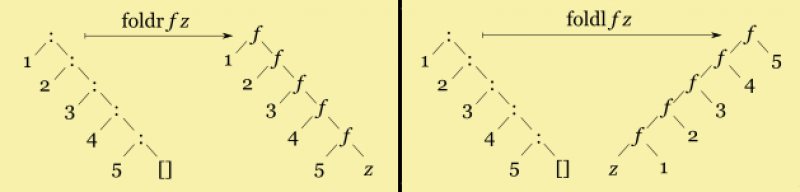
\includegraphics[max width=\textwidth]{:pp:fold-visualization.png}
\end{figure}
:


Tipurile acestor funcții sunt:


\begin{tcblisting}{ arc=0pt, outer arc=0pt, listing only, breakable}
Prelude> :t foldr
foldr :: (a -> b -> b) -> b -> [a] -> b
Prelude> :t foldl
foldl :: (a -> b -> a) -> a -> [b] -> a

\end{tcblisting}


\begin{tcolorbox}[colback=cyan!5, colframe=cyan!10, breakable]
Nu trebie să rețineți pe de rost tipurile. Încercați să înțelegeți ce exprimă și de ce sunt așa.
\end{tcolorbox}

Alte funcții de ordin superior des întâlnite: \texttt{map}, \texttt{filter}, \texttt{zipWith}, \texttt{flip}.


\subsection*{ Exerciții }

1. Fie două matrici reprezentate ca liste de liste. În rezolvarea exercițiilor de mai jos, puteți folosi doar funcții de ordin superior (împreună cu \texttt{take} și \texttt{drop}).

Implementați funcții care să returneze:

\begin{itemize}
	\item  linia \texttt{i} dintr-o matrice
	\item  elementul \texttt{(i, j)} dintr-o matrice
	\item  suma a două matrici
	\item  transpusa unei matrici 
	\item  produsul a două matrici
\end{itemize}


2. O imagine poate fi reprezentată ca o matrice de caractere (numiți, în continuare, "pixeli"). Considerăm că avem trei tipuri de pixeli: \texttt{'.'}, \texttt{'*'}, \texttt{' '}

Implementați următoarele funcții:
\begin{itemize}
	\item  flip orizontal, flip vertical, rotație de 90 în sens trigonometric și invers trigonometric
	\item  negativul (\texttt{'*'} si \texttt{'.'} devin \texttt{' '}, iar \texttt{' '} devine \texttt{'*'})
	\item  scalarea unei imagini cu \texttt{x} unități
	\item  alipirea a două imagini (cu aceeași înălțime) pe orizontală
	\item  alipirea a două imagini (cu aceeași lungime) pe verticală
	\item  crop orizontal de la de la coloana \texttt{x} la coloana \texttt{y}
	\item  crop vertical de la linia \texttt{x} la linia \texttt{y}
	\item  Implementați suprapunerea unei imagini peste o alta (având aceeași dimensiune)
\end{itemize}


\subsection*{ Resurse }

Puteți folosi următoarele pentru a vă testa funcțiile:


\begin{tcblisting}{ arc=0pt, outer arc=0pt, listing only, breakable}
l0="        ***** **            ***** **    "
l1="     ******  ****        ******  ****   "
l2="    **   *  *  ***      **   *  *  ***  "
l3="   *    *  *    ***    *    *  *    *** "
l4="       *  *      **        *  *      ** "
l5="      ** **      **       ** **      ** "
l6="      ** **      **       ** **      ** "
l7="    **** **      *      **** **      *  "
l8="   * *** **     *      * *** **     *   "
l9="      ** *******          ** *******    "
l10="      ** ******           ** ******     "
l11="      ** **               ** **         "
l12="      ** **               ** **         "
l13="      ** **               ** **         "
l14=" **   ** **          **   ** **         "
l15="***   *  *          ***   *  *          "
l16=" ***    *            ***    *           "
l17="  ******              ******            "
l18="    ***                 ***             "

img = [l0,l1,l2,l3,l4,l5,l6,l7,l8,l9,l10,l11,l12,l13,l14,l15,l16,l17,l18]

m1 = [[1, 2, 3], [4, 5, 6], [7, 8, 9]]
m2 = [[1, 0, 0], [0, 1, 1], [1, 0, 1]]

summ1m2 = [[2,2,3],[4,6,7],[8,8,10]]
prodm1m2 = [[4,2,5],[10,5,11],[16,8,17]]

-- functii care printeaza intr-un mod human-readable o matrice sau o imagine
display :: (Show a) => ([a] -> String) -> [[a]] -> IO ()
display displayLine = putStr . foldr (++) "" . map displayLine

-- folositi pentru a afisa o matrice de numere (ex. 1)
displayMat :: (Show a) => [[a]] -> IO ()
displayMat = display (foldr (\x acc -> show x ++ "   " ++ acc) "\n")

-- folositi pentru a afisa o "imagine" - matrice de siruri (ex. 2)
displayImg :: [String] -> IO ()
displayImg = display (++ "\n")


\end{tcblisting}

\section{ Course: Types in functional programming}
\section*{ Types in functional programming }

\subsection*{ Typing in programming languages }

\subsubsection*{ Strong vs weak typing }

Consider the following example from Javascript, where the operator \texttt{+} is applied on arguments of different types. The result is given below:

\begin{tcblisting}{ arc=0pt, outer arc=0pt, listing only, breakable}
[] + []  =  ""  
[] + {}  = "[object]"
{} + []  = 0
{} + {}  = null

\end{tcblisting}
 

where \texttt{[]} is the empty array and \texttt{\{\}} is the empty object. The result is quite surprising, and unpredictable. To explain it, we need to look at the implementation of the Javascript interpreter. In Javascript, there is a distinction between \textbf{primitive} and \textbf{non-primitive} values. Arrays (like \texttt{[]}) and objects (like \texttt{\{\}}) are considered non-primitive. Since the operation \texttt{+} is performed on primitive values, Javascript attempts to \textbf{convert} the operands to primitive. A pseudocode for this is shown below:

\begin{tcblisting}{ arc=0pt, outer arc=0pt, listing only, breakable}
     Convert(value) {
        if (value.valueOf() is a primitive) return it          //conversion to integer works?
        else if (value.toString() is a primitive) return it    //else convert to string, if possible 
             else error
     }

\end{tcblisting}


The conversion of \texttt{[]} to string yields the empty string, while the conversion of \texttt{\{\}} to string yields "[object]". This explains the first two results.

For the latter, we must know that \texttt{\{\}} can also be interpreted as a code-block, and this is the case here. Hence, the Javascript interpreter sees:

\begin{tcblisting}{ arc=0pt, outer arc=0pt, listing only, breakable} 
+ []
+ {}

\end{tcblisting}


where \texttt{+} is interpreted as a \textbf{unary} operator. JavaScript has such an implementation overloading for \texttt{+}. Without going into more details, \texttt{+ x} behaves like a \textit{conversion to Number} for x. Thus, \texttt{[]} converted to \texttt{Number} is \texttt{0}, while \texttt{\{\}} converted to \texttt{Number} is \texttt{NaN} (not a number).

\paragraph{ Morale }\hfill\\

The Javascript treatment of \texttt{+} is unimportant by itself, and it has some advantages for the programmer (although our example shows otherwise). However, we can note that, by allowing any \textbf{kind/type} of operand for \texttt{+}:
\begin{itemize}
	\item  \textbf{complicates the semantics} of the language (the programmer needs to known about conversion to primitives and conversion to numbers)
	\item  \textbf{reduces errors} (no Javascript error was signalled above), but \textbf{makes programs more prone to bugs}.
	\item  makes a program \textbf{more expressive} (\texttt{+} can be used in several ways) but sometimes difficult to use.
\end{itemize}


In programming language design, there is a fundamental tension between \textbf{expressiveness} and \textbf{typing}. Typing is a means for \textbf{enforcing constraints on what is deemed as a \textit{correct program}}. It may be the case that, \textit{conceptually correct} programs may not be accepted as \textbf{correct} from a typing perspective (this situation does seldom occur in Haskell).

A \textbf{strongly-typed} programming language, is more coercive with respect to \textbf{typing constraints}. In functional programming:
\begin{itemize}
	\item  Haskell
	\item  Scala
\end{itemize}
are considered \textbf{strongly-typed}. In imperative / OOP programming, the languages:
\begin{itemize}
	\item  Java
	\item  C++
	\item  Scala
\end{itemize}
are considered \textbf{strongly-typed}.

A \textbf{weakly-typed} programming language is more relaxed w.r.t. \textbf{typing constraints}. For instance, in functional programming:
\begin{itemize}
	\item  Racket (Lisp)
	\item  Clojure
\end{itemize}
are considered \textbf{weakly-typed}. In imperative / OOP programming, the languages:
\begin{itemize}
	\item  C
	\item  Python
	\item  PHP
	\item  Javascript
\end{itemize}

(and especially the latter) are considered weakly-typed. In the latter languages, types are usually reduced to primitive constructs (programmers cannot create new types), or the type construction procedure is very simplistic. For instance, in \texttt{Racket} (formerly known as \texttt{Scheme}), which weakly-typed:
\begin{itemize}
	\item  lists can hold any values (e.g.) \texttt{'(1 \#t "String")}, which means that the type for lists is \textbf{primitive} (not composed), and is simply \texttt{list}.
	\item  functions can return values of different types - the type for functions is also \textbf{primitive} - \texttt{\#procedure}. 
\end{itemize}

However, type verification is not absent in weakly-typed languages, including Racket/Scheme. For instance, the call \texttt{(+ 1 '())} will produce an error since the plus operator is called on values with invalid types.

We shall discuss Scheme/Racket in more detail later. It is worth noting that, in Racket there exists extensions (Typed Racket) which allow programmers to define and compose types to some extent.

The \textbf{weakly-typed} vs \textbf{strongly-typed} classification is not rigid and is subject to debate and discussion. There is no objective \textit{right-answer}. For instance, here, the language \texttt{C} is viewed as weakly-typed. We illustrate a small motivating example:


\begin{tcblisting}{ arc=0pt, outer arc=0pt, listing only, breakable}
int f (int x) {
    if (x != 0)
        return 1;
    return malloc(100);
}

\end{tcblisting}


In principle, the function \texttt{f} can return an integer, or a pointer to any object (of any type), and this is allowed by the compiler (which does issue a warning). Compared to, e.g. Java, this makes the \texttt{C} type system more relaxed.

There are valid arguments for considering \texttt{C} as strongly-typed and, as said before, there is no right answer.

\subsubsection*{ Compile-time vs runtime typing }

This classification is done w.r.t. \textbf{the moment} when type inference occurs:
\begin{itemize}
	\item  during the \textbf{compilation} of a program
	\item  at \textbf{runtime}
\end{itemize}

The former is also called \textbf{static typing}, while the latter - \textbf{dynamic typing}. In the literature, \textbf{static} and \textbf{dynamic} typing are also used with other meanings, hence, here, we prefer the terms \textbf{compile-time} and \textbf{runtime}.

The imperative/OOP languages:
\begin{itemize}
	\item  Java
	\item  Scala
	\item  C\textbackslash C++
\end{itemize}

perform compile-time type checking, as well as the functional languages:
\begin{itemize}
	\item  Haskell 
	\item  Scala
\end{itemize}

The imperative/OOP languages:
\begin{itemize}
	\item  Python
	\item  PHP
	\item  Javascript
\end{itemize}

perform runtime type checking, as well as the functional languages:
\begin{itemize}
	\item  Scheme/Racket (Lisp)
	\item  Clojure
\end{itemize}

Compile-time type checking is preferred for strongly-typed languages: the complexity of type verification is delegated to the compiler. Conversely, in weakly-typed languages, type verification is simpler, hence it can be performed by the interpreter, at runtime. Sometimes, a compiler may be absent. This is not a golden rule but merely an observation.

While runtime type checking is simpler to deploy, it has the disadvantage of not capturing typing bugs. Consider the following program in Racket:

\begin{tcblisting}{ arc=0pt, outer arc=0pt, listing only, breakable}
(define f (lambda (x) (if x 1 (+ 1 '()))))
(f #t)

\end{tcblisting}


The function receives a value \texttt{x} which must be a boolean. In the program above there is no error, even though \texttt{(+ 1 '())} is an incorrectly-typed function call. However, in the execution of the program (i.e. \texttt{(f \#t)}), the else branch of the function is not reached, hence no typing verification is performed.

Hence, runtime type checking only catches bugs \textbf{on the current program execution trace}.


\subsection*{ Typing in Haskell }

\subsection*{ Type inference in Haskell }

Haskell implements the \texttt{ Hindley-Milner type inference algorithm} \footnote{\url{https://en.wikipedia.org/wiki/Hindley\%E2\%80\%93Milner\_type\_system }}. In what follows, we present a simplified, and more easy-to-follow, but incomplete algorithm which serves as an illustration for the main concepts underlying the original one. 

\subsubsection*{ Intro }

Consider the following expressions, and their types:

\begin{tcblisting}{ arc=0pt, outer arc=0pt, listing only, breakable}
\x -> x + 1 :: Integer -> Integer
\x -> if x then 0 else 1 :: Bool -> Integer
zipWith (:) :: [a] -> [[a]] -> [[a]]
\f -> (f 1) + (f 2) :: (Integer -> Integer) -> Integer

\end{tcblisting}


We can see via the above example that types are constructed according to the following grammar:


\begin{tcblisting}{ arc=0pt, outer arc=0pt, listing only, breakable}
type ::= <const_type> | <type_var> | (<type>) | type -> type | [<type>]

\end{tcblisting}


This grammar only tells half the story regarding Haskell typing, however, for the purposes of this lecture, this view suffices. According to the above grammar, types can be:
\begin{itemize}
	\item  \textbf{constant types} (e.g. \texttt{Integer}, \texttt{String})
	\item  \textbf{type variables} (e.g. \texttt{a} - which are usually used to designate \textbf{any} possible type, as in \texttt{[a]})
	\item  \textbf{function types} (e.g. \texttt{Integer -\textgreater  Integer} or \texttt{(Integer -\textgreater  Integer)} if this type appears in a larger type expression)
	\item  \textbf{list types} (e.g. \texttt{[a]}).
	\item  any combination of the above rules.
\end{itemize}


\subsubsection*{ Expression trees }

We assume each Haskell expression is constructed via the following \textit{construction rules}:
\begin{itemize}
	\item  \textbf{functional application} (e.g. \texttt{take 2 [1,2,3]})
	\item  \textbf{function definition} (e.g. \texttt{\textbackslash x-\textgreater [x+1]})
\end{itemize}

We note that many Haskell definitions can be seen as such. For instance:

\begin{tcblisting}{ arc=0pt, outer arc=0pt, listing only, breakable}
g f = (f 1) + 1
<code>

can be seen as:

<code haskell>
g = \f -> (f 1) + 1

\end{tcblisting}


Hence, we can take any Haskell expression, and construct a \textbf{tree}, in which each node represents a \textbf{construction rule}, and children represent sub-expressions:
\begin{itemize}
	\item  for functional applications, the children are the \textbf{function name} and \textbf{the parameters}
	\item  for function definition, the children are \textbf{the variable/variables} and the \textbf{function body}.
\end{itemize}

For example, consider the expression tree for the function \texttt{g} shown previously (we use tabs to illustrate parent/child relationship):

\begin{tcblisting}{ arc=0pt, outer arc=0pt, listing only, breakable}
\f -> (f 1) + 1
  f
  (f 1) + 1
    (+)
    (f 1)
       f 
       1
    1

\end{tcblisting}


In what follows, we shall use expression trees to perform type inference.

\subsubsection*{ Typing rules }

We introduce the following \textbf{typing rules}:

\paragraph{ Rule (TVar) }\hfill\\

If \texttt{v} is bound to a constant expression e of type \texttt{ct}, then \texttt{v :: ct}

\paragraph{ Rule (TFun) }\hfill\\

If \texttt{x :: t1} and \texttt{e :: t2} then \texttt{\textbackslash x -\textgreater  e  :: t1 -\textgreater  t2}

\paragraph{ Rule (TApp) }\hfill\\

If \texttt{f :: t1 -\textgreater  t2} and \texttt{e :: t1} then \texttt{(f e) :: t2}

The above rule can be naturally generalised:

If \texttt{f :: t1 -\textgreater  t2 -\textgreater  ... -\textgreater  tn -\textgreater  t} and \texttt{e1 :: t1}, ..., \texttt{en :: tn} then \texttt{(f e1 ... en) :: t}

In what follows, we will use these rules to make judgements on our types. These rules have a twofold usage:
\begin{itemize}
	\item  \textbf{deduce} the type of an expression, based on \textit{existing knowledge}
	\item  \textbf{make hypotheses} regarding the type of an expression (we shall not focus on this aspect in the presentation))
\end{itemize}

\subsubsection*{ Type inference stage 1: Expression tree construction }

Type inference for an expression \texttt{e} can be seen as having two stages. In the first stage, we:
\begin{itemize}
	\item  construct the expression tree of \texttt{e}
	\item  make \textbf{hypotheses} regarding the types of \textbf{yet untyped} expressions (e.g. variables).
\end{itemize}

We illustrate the first stage on the previous definition of \texttt{g}:


\begin{tcblisting}{ arc=0pt, outer arc=0pt, listing only, breakable}
\f -> (f 1) + 1 :: ?
  f :: tf (here we introduce tf as the type of f. This is a type hypothesis)
  (f 1) + 1 :: ?
    (+) :: ?
    (f 1) :: ?
       f :: t1 -> t2 (this is another hypothesis, stemming from the fact that f is applied on 1)
       1 :: ?
    1 :: ?

\end{tcblisting}


\subsubsection*{ Type inference stage 2: Rule application }

In this stage, we start from the previously-build tree, and:
\begin{itemize}
	\item  \textbf{apply typing rules} to deduce types for new sub-expressions
	\item  \textbf{perform type unification}: This is one aspect that we shall not elaborate on, in this lecture. 
\end{itemize}

This is equivalent to a \textbf{bottom-up} tree traversal: We start from the leaves, and progress to the root (i.e. the expression to be typed).

Without delving into details, \textbf{type unification} is an important ingredient, because it allows us to infer \textbf{the most general} type of an expression. Consider the following Haskell expression: \texttt{\textbackslash f x -\textgreater  (f x,f 1)}, which defines a function that takes another function \texttt{f}, a value \texttt{x} and returns a pair: the first element of the pair is the application \texttt{f x}, while the second - \texttt{f 1}:
\begin{itemize}
	\item  initially, we do not know what \texttt{f} is, hence it has \textbf{the most general type} (say) \texttt{tf} - it can be anything;
	\item  judging by the application \texttt{f x}, we deduce that \texttt{f} must be a function, of type \texttt{a-\textgreater b}, where \texttt{x::a}
	\item  judging by the application \texttt{f 1}, we deduce that \texttt{a} must be an \texttt{Integer}
\end{itemize}
The unification process combines the information collected so far:
\begin{itemize}
	\item  \texttt{tf} must unify (coincide with) \texttt{a -\textgreater  b}
	\item  \texttt{a} must unify with \texttt{Integer}
\end{itemize}

The final type for the expression is: \texttt{(Integer -\textgreater  b) -\textgreater  Integer -\textgreater  (b, b)}

We illustrate the second stage of the type inference on the same example:


\begin{tcblisting}{ arc=0pt, outer arc=0pt, listing only, breakable}
\f -> (f 1) + 1 :: tf -> Integer
  f :: tf (via (TFun))
  (f 1) + 1 :: Integer (via (TApp))
    (+) :: Integer -> Integer -> Integer (this we know from Prelude, after the type synthesis of (+), also t2 must unify with Integer)
    (f 1) :: t2 (via (TApp); also, t1 must unify with Integer)
       f :: t1 -> t2
       1 :: Integer (via (TVar), from Prelude)
    1 :: Integer (via (TVar), from Prelude)

\end{tcblisting}


The (pseudo)-algorithmic procedure concludes with the following answer:
\begin{itemize}
	\item  \texttt{g :: tf -\textgreater  Integer}, where

  \begin{itemize}
  	\item  \texttt{tf} unifies with \texttt{t1 -\textgreater  t2}
  	\item  \texttt{t2} unifies with \texttt{Integer}
  	\item  \texttt{t1} unifies with \texttt{Integer}
  \end{itemize}
\end{itemize}

After unification, the result is shown to the programmer: \texttt{ g :: (Integer -\textgreater  Integer) -\textgreater  Integer}

Exercises. Find the type of the following expressions, by applying the type synthesis pseudo-algorithm:
\begin{itemize}
	\item  \texttt{map (\textbackslash x-\textgreater [x+1])}
	\item  \texttt{\textbackslash f x-\textgreater  if x then f x else x}
	\item  \texttt{g f x = x \&\& (f x)}
	\item  \texttt{g f = f (g f)}
\end{itemize}


\section{ Course: Abstract datatypes}
\subsection*{ Abstract Datatypes }

\subsubsection*{ Intro }

An Abstract Datatype relies on \textit{functions} to describe the possible values of a type. We start with a simplistic example:


\begin{tcblisting}{ arc=0pt, outer arc=0pt, listing only, breakable}
data Nat = Zero | Succ Nat

\end{tcblisting}

\begin{itemize}
	\item  the expression \texttt{data Nat} introduces a new \textbf{type} in the programming language
	\item  after \texttt{=}, the \textbf{base constructors} of the type follow. In Haskell, \textbf{all constructors} must begin with a capital letter
	\item  \texttt{Zero} is a nullary constructor. 
	\item  \texttt{Succ Nat} designates an \textbf{internal} constructor, which expects a natural number (of type \texttt{Nat}). A value \texttt{(Succ x)} \textbf{is} of type \texttt{Nat} (i.e. a natural number), and we may be tempted to see it as a function call, which \textit{returns} the successor of \texttt{x}
\end{itemize}

\texttt{Zero} and \texttt{Succ} are called \textbf{data constructors} in Haskell. \texttt{Nat} is called a \texttt{type} or \texttt{type-constructor}. We shall distinguish between the two in a later lecture.

Note that the \textit{internal} representation of an ADT, as perceived by the programmer, is \textit{abstract}. We may see values as \textit{calls} of special functions - data constructors. Except for their meaning (and language-level implementation), data constructors behave exactly as functions. For instance:
\begin{itemize}
	\item  \texttt{Zero :: Nat}
	\item  \texttt{Succ :: Nat -\textgreater  Nat}
\end{itemize}

We continue the example with addition:


\begin{tcblisting}{ arc=0pt, outer arc=0pt, listing only, breakable}
add :: Nat -> Nat -> Nat
add Zero y = y
add (Succ x) y = Succ (add x y)

\end{tcblisting}


An important observation is that the \textbf{pattern matching mechanism} in Haskell relies on data constructors, and their applications. For instance, the following definition is a correct usage of the pattern matching mechanism:

\begin{tcblisting}{ arc=0pt, outer arc=0pt, listing only, breakable}
f (1:y:[]) = ...

\end{tcblisting}

I uses the data constructors \texttt{(:)} and \texttt{[]} for lists, as well as the data constructor \texttt{1} for integers. The pattern describes any list of integers which starts with a \texttt{1} and contains exactly two elements.

\subsubsection*{ Monomorphic List implementation }

In what follows, we give an implementation for the type \textit{List of integers}. This type is called \textit{monomorphic}, since our list can only contain elements of a single type (integer):


\begin{tcblisting}{ arc=0pt, outer arc=0pt, listing only, breakable}
data IList = Void | Cons Integer IList

app :: IList -> IList -> IList
app Void l = l
app (Cons h t) l = Cons h (app t l)

convert :: IList -> [Integer]
convert Void = []
convert (Cons h t) = h : (convert t)

mfoldl :: (b -> Integer -> b) -> b -> IList -> b
mfoldl op acc Void = acc
mfoldl op acc (Cons h t) = mfoldl op (op acc h) t

mfoldr :: (Integer -> a -> a) -> a -> IList -> a
mfoldr op acc Void = acc
mfoldr op acc (Cons h t) = op h (mfoldr op acc t)

convert2 :: IList -> [Integer]
convert2 = mfoldr (:) []

showl :: IList -> String
showl = show . convert2


\end{tcblisting}


In the above code, we have defined some basic list operations, such as \texttt{app} (list concatenation) and \texttt{convert}, which transforms a list of type \texttt{IList} to a conventional Haskell list (of type \texttt{[Integer]}).

We have also implemented the two folding procedures for \texttt{IList}. Note the type signature of each fold. Finally, we have used folds to provide an alternative implementation for convert, as well as for converting lists to strings.


\subsubsection*{ Propositional Logic in Haskell }

Abstract Datatypes are a natural way to define more elaborate data-structures, such as propositional formulae. We give a possible definition below:


\begin{tcblisting}{ arc=0pt, outer arc=0pt, listing only, breakable}
data Formula = Var String | And Formula Formula | Or Formula Formula | Not Formula

\end{tcblisting}


We observe that:
\begin{itemize}
	\item  \texttt{Var :: String -\textgreater  Formula}
	\item  \texttt{And :: Formula -\textgreater  Formula -\textgreater  Formula}
	\item  \texttt{Or :: Formula -\textgreater  Formula -\textgreater  Formula}
	\item  \texttt{Not :: Formula -\textgreater  Formula}
\end{itemize}

A good exercise consists in the implementation of a display function for formulae:

\begin{tcblisting}{ arc=0pt, outer arc=0pt, listing only, breakable}
fshow :: Formula -> String
fshow (Var v) = v
fshow (And f1 f2) = "("++(fshow f1)++" ^ "++(fshow f2)++")"
fshow (Or f1 f2) = "("++(fshow f1)++" V "++(fshow f2)++")"
fshow (Not f) = "~("++(fshow f)++")"

\end{tcblisting}


Next, we implement a function \texttt{push}, which pushes negation \textit{inward}:

\begin{tcblisting}{ arc=0pt, outer arc=0pt, listing only, breakable}
push :: Formula -> Formula
push (Var v) = (Var v)
push (Not (Var v)) = Not (Var v)
push (Not (And f1 f2)) = Or (push (Not f1)) (push (Not f2))
push (Not (Or f1 f2)) = And (push (Not f1)) (push (Not f2))
push (And f1 f2) = And (push f1) (push f2)
push (Or f1 f2) = Or (push f1) (push f2)

\end{tcblisting}


Notice, at lines 4,5 the implementation of deMorgan's laws.

Finally, we implement a function which computes the truth-value of a formula, under a certain interpretation. First, we define the type \texttt{Interpretation}:

\begin{tcblisting}{ arc=0pt, outer arc=0pt, listing only, breakable}
type Interpretation = String -> Bool

i :: Interpretation
i "x" = True
i "y" = False
i "z" = True

\end{tcblisting}
 

In the first line, we have defined a \textbf{type-alias}: \texttt{Interpretation} is a function from strings to booleans. We have also implemented a three-variable interpretation, for testing purposes. Next, we implement \texttt{eval}:


\begin{tcblisting}{ arc=0pt, outer arc=0pt, listing only, breakable}
eval :: Interpretation -> Formula -> Bool
eval i (Var v) = i v
eval i (Not f) = not(eval i f)
eval i (And f1 f2) = (eval i f1) &\&&&\&& (eval i f2)
eval i (Or f1 f2) = (eval i f1) || (eval i f2)

\end{tcblisting}


\subsubsection*{ Monomorphic Trees in Haskell }


\begin{tcblisting}{ arc=0pt, outer arc=0pt, listing only, breakable}
data ITree = Leaf | Node ITree Integer ITree

\end{tcblisting}


Note that:
\begin{itemize}
	\item  \texttt{Leaf :: ITree}
	\item  \texttt{Node :: ITree -\textgreater  Integer -\textgreater  ITree -\textgreater  ITree}
\end{itemize}

Next, we implement a folding operation on Trees. The key to it is to conceptually define what folding should do on Trees. To grasp an intuition, recall that: 
\begin{itemize}
	\item  \texttt{foldr (:) []} is the \textbf{identity function} on lists. Hence, \texttt{foldr (:) [] [1,2,3]} produces \texttt{[1,2,3]}.
	\item  also, recall that the map operation can be defined as: \texttt{\textbackslash f -\textgreater  foldr ((:).f) []}
\end{itemize}

Similar to the list case, a fold on trees should:
\begin{itemize}
	\item  \textbf{preserve the tree structure}, given the appropriate operator (e.g. \texttt{Node}). 
	\item  hence, the call \texttt{mtfold Node Leaf} (where \texttt{Leaf} is the accumulator) should be the \textbf{identity function on trees}. 
\end{itemize}

Let us define the identity function \texttt{tid} for trees:

\begin{tcblisting}{ arc=0pt, outer arc=0pt, listing only, breakable}
tid Leaf = Leaf
tid (Node r k l) = Node (tid r) k (tid l)

\end{tcblisting}


As already said, \texttt{(tid t)} is equivalent to the call \texttt{(mtfold Node Leaf t)}, for any arbitrary tree \texttt{t}.
To obtain the general \texttt{mtfold} implementation, we simply generalise \texttt{Node} by an arbitrary operation \texttt{op}:
\begin{itemize}
	\item  if \texttt{Node :: ITree -\textgreater  Integer -\textgreater  ITree -\textgreater  ITree}, then
	\item  \texttt{op :: b -\textgreater  Integer -\textgreater  b -\textgreater  b}
\end{itemize}

We also generalise \texttt{Leaf} by an arbitrary accumulator:
\begin{itemize}
	\item  if \texttt{Leaf :: ITree} then
	\item  \texttt{acc :: b}
\end{itemize}

The code generalisation becomes:


\begin{tcblisting}{ arc=0pt, outer arc=0pt, listing only, breakable}
mtfold :: (b -> Integer -> b -> b) -> b -> ITree -> b
mtfold op acc = 
    let f (Node left key right) = f (f left) key (f right)
        f Leaf = acc
    in f

\end{tcblisting}


Notice that \texttt{f} is precisely the generalisation of \texttt{tid} according to our observations. We can use \texttt{mtfold} to implement various tree operations such as:


\begin{tcblisting}{ arc=0pt, outer arc=0pt, listing only, breakable}
tsum = mtfold (\k r l->k + r + l) 0 
tmirror = mtfold (\k r l -> Node l k r) Leaf 
tflatten = mtfold (\k r l -> r ++ [k] ++ l) [] 

\end{tcblisting}
 
\subsection{ Lab: Abstract datatypes}
\section*{ Tipuri de date abstracte }

Scopul laboratorului:
\begin{itemize}
	\item  Recapitularea conceptului de TDA
	\item  Definirea de TDA-uri în Haskell
	\item  Familiarizarea cu conceptul de TDA-uri polimorfice
	\item  Introducerea tipului de date \texttt{Maybe}
\end{itemize}


\subsection*{ Tipuri de date abstracte (TDA) }

\textbf{Tipurile de date abstracte} sunt modele pentru a defini tipuri de date în funcție de comportamentul acestora (valori posibile, axiome, operații), contrastând cu \textit{structurile de date}, definite din punct de vedere al implementării.

Un TDA familiar este \textbf{list}. \\Pentru a lucra cu liste într-un limbaj ca Java, am scris două \textit{implementări} distincte, și anume \texttt{LinkedList} și \texttt{ArrayList}. Ambele implementări respectă specificațiile din primul paragraf.

\begin{tcolorbox}[colback=yellow!40, colframe=yellow!60, breakable]
Unii autori includ în descrierea TDA-urilor și complexități. Din acest punct de vedere, implementările 
\texttt{LinkedList} și \texttt{ArrayList} diferă.
\end{tcolorbox}


\subsubsection*{ Constructori }

Valorile posibile ale unui TDA sunt date de constructorii acestuia.\\Să considerăm un tip simplu de date: \texttt{Bool}, care poate avea două valori: \texttt{False} și \texttt{True}.\\Sintaxa Haskell pentru a defini acest tip de date este următoarea:


\begin{tcblisting}{ arc=0pt, outer arc=0pt, listing only, breakable}
data Bool = False | True

\end{tcblisting}


\begin{tcolorbox}[colback=yellow!40, colframe=yellow!60, breakable]
Atât numele tipului de date cât și numele constructorilor trebuie scris cu literă mare.
\end{tcolorbox}

\texttt{False} și \texttt{True} nu sunt parametrizate și pot fi privite ca valori. Se mai numesc și \textit{constructori nulari}.\\
Să considerăm un alt TDA care descrie un arbore binar cu valori întregi. Arborele poate fi gol sau un nod cu doi copii.


\begin{tcblisting}{ arc=0pt, outer arc=0pt, listing only, breakable}
data Tree = Nil | Node Int Tree Tree

\end{tcblisting}


\texttt{Node} este un constructor care primește un argument de tipul \texttt{Int} și două argumente de tip \texttt{Tree}, pentru a creea o valoare de tip \texttt{Tree}. Putem să ne gândim la el ca la o funcție:


\begin{tcblisting}{ arc=0pt, outer arc=0pt, listing only, breakable}
Prelude> :t Node
Node :: Int -> Tree -> Tree -> Tree

\end{tcblisting}


Constructorii sunt foarte importanți în \textit{pattern matching}. Ca exemplu, vom scrie o funcție care însumează toate valorile dintr-un arbore:


\begin{tcblisting}{ arc=0pt, outer arc=0pt, listing only, breakable}
treeSum :: Tree -> Int
treeSum Nil = 0
treeSum (Node v l r) = v + (treeSum l) + (treeSum r)

\end{tcblisting}


Observăm prezența a două pattern-uri: unul pentru arborele vid, celălalt pentru un nod, într-un fel foarte asemănător cu modul în care lucram cu liste, făcând pattern matching pe \texttt{[]} și \texttt{(x:xs)}.

\begin{tcolorbox}[colback=cyan!5, colframe=cyan!10, breakable]
Observați că ghci nu știe cum să afișeze arborele nostru:


\begin{tcblisting}{ arc=0pt, outer arc=0pt, listing only, breakable}
Prelude> Node 1 Nil Nil

<interactive>:38:1:
    No instance for (Show Tree) arising from a use of 'print'
    In a stmt of an interactive GHCi command: print it

\end{tcblisting}


Pentru a vă fi mai ușor să vă verificați, puteți obține o reprezentare a tipurilor definite de voi astfel:


\begin{tcblisting}{ arc=0pt, outer arc=0pt, listing only, breakable}
data Tree = Nil | Node Int Tree Tree deriving (Show)

\end{tcblisting}


Pe scurt, acest lucru înrolează TDA-ul vostru în clasa \texttt{Show}, oferind o implementare implicită a funcției \texttt{show} (apelată de ghci). Mai multe detalii în laboratorul următor.


\begin{tcblisting}{ arc=0pt, outer arc=0pt, listing only, breakable}
Prelude> Node 1 Nil Nil
Node 1 Nil Nil

\end{tcblisting}

\end{tcolorbox}


\subsubsection*{ Înregistrări }

Vrem să definim un TDA pentru a descrie un student, folosind următoarele câmpuri: nume, prenume, an de studiu, medie.


\begin{tcblisting}{ arc=0pt, outer arc=0pt, listing only, breakable}
-- tipul de date si constructorul au acelasi nume, ceea ce este ok
-- pentru ca reprezinta concepte diferite.
data Student = Student String String Int Float

\end{tcblisting}


Observăm că semnficația câmpurilor nu este evidentă din definiție. Vrem să extragem valori dintr-un Student; definim funcțiile:


\begin{tcblisting}{ arc=0pt, outer arc=0pt, listing only, breakable}
nume :: Student -> String
nume (Student n _ _ _) = n

prenume :: Student -> String
prenume (Student _ p _ _) = p

an :: Student -> Int
an (Student _ _ a _) = a

medie :: Student -> Float
medie (Student _ _ _ m) = m

\end{tcblisting}


Pentru a face descrierea tipului de date mai clară și a evita să scriem manual acele funcții, putem folosi sintaxa:


\begin{tcblisting}{ arc=0pt, outer arc=0pt, listing only, breakable}
data Student = Student { nume :: String
                       , prenume :: String
                       , an :: Int
                       , medie :: Float
                       }

\end{tcblisting}

                      


\subsection*{ TDA-uri polimorfice }

Până acum, am definit TDA-uri care lucrează doar cu întregi. Dorim să scăpăm de această limitare și să definim TDA-uri care pot lucra cu orice alt tip de date. De exemplu, are sens să considerăm capul unei liste care conține elemente de tip \texttt{a}, ca fiind un element de tip \texttt{a}, indiferent de cum arată acest tip.\\
Într-adevăr, aceasta este definiția funcției \texttt{head} existentă în Haskell:


\begin{tcblisting}{ arc=0pt, outer arc=0pt, listing only, breakable}
Prelude> :t head
head :: [a] -> a

\end{tcblisting}


\texttt{a} se numește \textbf{variabilă de tip} și poate să reprezinte orice tip de date (evident, cu condiția ca toate \texttt{a}-urile care apar să se refere la același tip).

\begin{tcolorbox}[colback=blue!10, colframe=blue!20]
Să ne uităm la tipul altei funcții cunoscute:


\begin{tcblisting}{ arc=0pt, outer arc=0pt, listing only, breakable}
Prelude> :t map
map :: (a -> b) -> [a] -> [b]

\end{tcblisting}


\texttt{map} primește ca argument o funcție - care primește un element de tip \texttt{a} și întoarce un element de tip \texttt{b} - și o listă de elemente de tip \texttt{a} și întoarce o listă de elemente de tip \texttt{b}. De precizat că \texttt{a} și \texttt{b} pot fi distincte dar nu este necesar.
\end{tcolorbox}

Listele din Haskell sunt \textbf{polimorfice}. Ele pot conține date de orice tip. O instanță a listelor are însă un tip concret:


\begin{tcblisting}{ arc=0pt, outer arc=0pt, listing only, breakable}
Prelude> :t ['a', 'b', 'c']
['a', 'b', 'c'] :: [Char]

\end{tcblisting}


\subsubsection*{ Constante polimorfice }

Care este tipul listei vide?


\begin{tcblisting}{ arc=0pt, outer arc=0pt, listing only, breakable}
Prelude> :t []
[] :: [a]

\end{tcblisting}


Observăm că tipul listei vide este general. Asta înseamnă că lista vidă poate fi tratată ca o listă de orice tip.


\begin{tcblisting}{ arc=0pt, outer arc=0pt, listing only, breakable}
Prelude> [1,2,3] ++ "123" -- eroare, tipuri diferite
Prelude> [1,2,3] ++ []
[1,2,3]
Prelude> "123" ++ []
"123"

\end{tcblisting}


Spunem că \texttt{[]} este o \textbf{constantă polimorfică}.

\begin{tcolorbox}[colback=blue!10, colframe=blue!20]
O altă constantă polimorfică este, de exemplu \texttt{1}. De aceea putem scrie:


\begin{tcblisting}{ arc=0pt, outer arc=0pt, listing only, breakable}
Prelude> 1 + 2
3
Prelude> 1 + 2.71
3.71

\end{tcblisting}


Dacă forțăm 1 să fie întreg, vom primi o eroare la a doua adunare:

\begin{tcblisting}{ arc=0pt, outer arc=0pt, listing only, breakable}
Prelude> (1 :: Int) + 2.71

<interactive>:60:14:
    No instance for (Fractional Int) arising from the literal '2.71'
    In the second argument of '(+)', namely '2.71'
    In the expression: (1 :: Int) + 2.71
    In an equation for 'it': it = (1 :: Int) + 2.71

\end{tcblisting}


\texttt{1} are însă o constrângere despre care vom discuta în laboratorul următor.
\end{tcolorbox}


Pentru a implementa în Haskell un TDA polimorfic, folosim sintaxa:


\begin{tcblisting}{ arc=0pt, outer arc=0pt, listing only, breakable}
data List a = Empty | Cons a (List a)

\end{tcblisting}


\begin{tcolorbox}[colback=blue!10, colframe=blue!20]
Ce este \texttt{List}?\\
\texttt{List} este un \textbf{constructor de tip}, nu un tip de date. Constructorii de tip primesc ca parametrii \textit{tipuri} și întorc un tip (sau un alt constructor de tip dacă nu primesc suficienți parametrii).\\Asta înseamnă că, \texttt{List} nu este un \textit{tip}, dar \texttt{List Int}, \texttt{List Char} etc. sunt tipuri.
\end{tcolorbox}

\subsubsection*{ Maybe și Either }

Unul dintre TDA-urile puse la dispoziție de Haskell este \texttt{Maybe}, un tip \textit{polimorfic} care modelează prezența unei anumite valori, sau absența acesteia:

\begin{tcblisting}{ arc=0pt, outer arc=0pt, listing only, breakable}
data Maybe a = Nothing | Just a

\end{tcblisting}


Pentru a ilustra importanța acestui TDA, considerăm următoare situație: vrem să implementăm o funcție care returnează suma valoriilor celor doi copii ai unui nod dat:


\begin{tcblisting}{ arc=0pt, outer arc=0pt, listing only, breakable}
childrenSum :: Tree -> Maybe Int
childrenSum Nil = Nothing
childrenSum (Node _ Nil _) = Nothing
childrenSum (Node _ _ Nil) = Nothing
childrenSum (Node _ (Node v _ _) (Node w _ _)) = Just (v + w)

\end{tcblisting}


Această sumă există doar pentru arbore diferit de Nil, cu ambii copii diferiți de Nil.

Putem scrie o funcție care ia un \texttt{Maybe} și returnează un șir pentru printare. Combinăm apoi cele două funcții:


\begin{tcblisting}{ arc=0pt, outer arc=0pt, listing only, breakable}
pretty :: Maybe Int -> String
pretty Nothing = "No value"
pretty (Just v) = "Sum is " ++ show v

printChildrenSum :: Tree -> String
printChildrenSum = pretty . childrenSum

\end{tcblisting}


Încărcăm modulele în ghci și voilà:

\begin{tcblisting}{ arc=0pt, outer arc=0pt, listing only, breakable}
*Main> printChildrenSum (Node 1 (Node 1 Nil (Node 2 Nil Nil)) (Node 3 (Node 4 (Node 5 Nil Nil) Nil) (Node 6 Nil Nil)))
"Sum is 4"
*Main> printChildrenSum Nil
"No value"
*Main> printChildrenSum (Node 1 Nil (Node 1 Nil Nil))
"No value"
*Main> printChildrenSum (Node 1 (Node 1 Nil Nil) Nil)
"No value"

\end{tcblisting}


Un TDA similar este \texttt{Either}, care modelează valori cu două tipuri posibile:


\begin{tcblisting}{ arc=0pt, outer arc=0pt, listing only, breakable}
data Either a b = Left a | Right b

\end{tcblisting}


Prin convenție, constructorul \texttt{Left} reprezintă o eroare, iar constructorul \texttt{Right} o valoare corectă. Astfel putem extinde mecanisme de error-handling pentru a conține mai multe informații despre ce a cauzat eroarea (spre deosebire de \texttt{Maybe}, care doar indică \textbf{existența} unei erori):


\begin{tcblisting}{ arc=0pt, outer arc=0pt, listing only, breakable}
childrenSum :: Tree -> Either String Int
childrenSum Nil = Left "Tree is Nil"
childrenSum (Node _ Nil _) = Left "Left child is Nil"
childrenSum (Node _ _ Nil) = Left "Right child is Nil"
childrenSum (Node _ (Node v _ _) (Node w _ _)) = Right (v + w)

pretty :: Either String Int -> String
pretty (Left s) = s
pretty (Right i) = "Sum is " ++ show i

printChildrenSum :: Tree -> String
printChildrenSum = pretty . childrenSum

\end{tcblisting}



\begin{tcblisting}{ arc=0pt, outer arc=0pt, listing only, breakable}
*Main> printChildrenSum (Node 1 (Node 1 Nil (Node 2 Nil Nil)) (Node 3 (Node 4 (Node 5 Nil Nil) Nil) (Node 6 Nil Nil)))
"Sum is 4"
*Main> printChildrenSum Nil
"Tree is Nil"
*Main> printChildrenSum (Node 1 Nil (Node 1 Nil Nil))
"Left child is Nil"
*Main> printChildrenSum (Node 1 (Node 1 Nil Nil) Nil)
"Right child is Nil"

\end{tcblisting}


\subsubsection*{ Exerciții }

\begin{tcolorbox}[colback=yellow!40, colframe=yellow!60, breakable]
Încercați să vă obișnuiți să scrieți explicit tipurile tuturor funcțiilor definite de voi în continuare.
\end{tcolorbox}

\subparagraph{ 1. List }\hfill\\

a) implementați TDA-ul pentru propria voastră listă care poate conține doar numere întregi\\b) scrieți o funcție care convertește valori ale TDA-ului vostru în liste din Haskell

\begin{tcolorbox}[colback=cyan!5, colframe=cyan!10, breakable]
Dacă tipul vostru de listă se numește \texttt{List}, atunci tipul funcției va fi: 


\begin{tcblisting}{ arc=0pt, outer arc=0pt, listing only, breakable}
convertList :: List -> [Int]

\end{tcblisting}

\end{tcolorbox}

c) modificați tipul \texttt{List} pentru a fi polimorfic, apoi modificați și funcția \texttt{convertList}

\subparagraph{ 2. Tree }\hfill\\
a) Implementați TDA-ul pentru arbori polimorfici.\\b) Implementați \texttt{foldT}, echivalentul lui \texttt{foldr} (puteți vizualiza rezultatul ca fiind înlocuirea tuturor constructorilor nulari cu o valoare constantă și a tuturor celorlalți constructori cu funcții care iau același numă de argumente.\\c) Implementați o funcție \texttt{mapT} (echivalentul lui \texttt{map}), folosindu-vă de \texttt{foldT}.\\d) Implementați o funcție \texttt{zipWithT} (echivalentul lui \texttt{zipWith}).\\
\subparagraph{ 3. Numere naturale extinse }\hfill\\
a) Implementați un TDA care să modeleze numere naturale extinse cu un punct la infinit ($ \hat{\mathbb{N}} = \mathbb{N} \cup \{ \infty \}$).\\b) Implementați o funcție \texttt{extSum} care să evalueze suma a două numere naturale extinse.\\c) Implementați o funcție \texttt{extDiv} care să evalueze raportul a două numere naturale extinse (împărțirea la 0 și la infinit are rezultat definit).\\d) Implementați o funcție \texttt{extLess} care spune dacă un număr natural extins e mai mic decât un altul.

În laboratorul următor, vom vedea cum putem implementa aceste operații într-un mod consistent cu restul limbajului, folosind operatori cunoscuți (\texttt{+}, \texttt{div}, \texttt{\textless }).
                   
\subparagraph{ 4. Înregistrări }\hfill\\

a) Scrieți un TDA care codifică un tuplu (înregistrare) format din următoarele câmpuri:
   \begin{itemize}
   	\item  Nume (codificat ca String)
   	\item  Vârstă (codificat ca Integer)
   	\item  Prieteni (codificat ca o lista de String-uri)
   	\item  Notă PP (codificat ca Integer). Acest câmp este opțional!
   \end{itemize}

b) Scrieți o funcție care primește o listă de înregistrări și le întoarce pe acelea pentru care vârsta este mai mare ca 20.\\c) Scrieți o funcție care primește o listă de înregistrări și le întoarce pe acelea care conțin cel puțin un prieten cu numele "Matei".\\d) Scrieți o funcție care primește o listă de înregistrări și le întoarce pe acelea care conțin câmpul "Notă PP".\\e) Scrieți o funcție care primește o listă de nume, o listă de vârste, o listă ce conține liste de prieteni, și întoarce o listă de înregistrări corespunzătoare.

\subsection*{ Referințe }

\begin{itemize}
	\item  \texttt{Abstract Data Type - Haskell wiki} \footnote{\url{https://wiki.haskell.org/Abstract\_data\_type}}
	\item  \texttt{Algebraic Data Type - Haskell wiki} \footnote{\url{https://wiki.haskell.org/Algebraic\_data\_type}}
	\item  \texttt{Maybe - Haskell wiki} \footnote{\url{https://wiki.haskell.org/Maybe}}
\end{itemize}

\section{ Course: Polymorphism in functional languages}
\section*{ Polymorphism in functional languages }

\subsection*{ Polymorphism in Object-Oriented languages }

Translated literally, the term \textbf{polymorphism} means \textbf{multiple shapes}. Polymorphism in programming languages is a powerful modularisation tool, which allows programmers to:
\begin{itemize}
	\item  \textbf{abstract from implementation details} (in the case of ad-hoc polymorphism)
	\item  \textbf{define a unique implementation for a range of types} (in the case of parametric polymorphism / genericity)
\end{itemize}

Polymorphism is a mechanism supported by virtually any strongly-typed programming language, including functional and object-oriented ones.

\subsubsection*{ Ad-hoc polymorphism }

In an Object-Oriented language (say, Java), \textbf{ad-hoc polymorphism} allows the programmer to \textit{(dynamically) select the implementation of a function, based on the type(s) of the variable(s) on which the former is applied}.

Consider the following class definitions:

\begin{tcblisting}{ arc=0pt, outer arc=0pt, listing only, breakable}
class Animal {
  public void talk (){
    System.out.println("I am an Animal");
  }
}

class Bird extends Animal {
  public void talk (){
    System.out.println("Cip-cirip");
  }
}

\end{tcblisting}


Finally, consider the following code:

\begin{tcblisting}{ arc=0pt, outer arc=0pt, listing only, breakable}
 Animal [] v = new Animal [2];
    v[0] = new Animal();
    v[1] = new Bird();
    for (Animal a:v)
      a.talk();

\end{tcblisting}


whose output is:

\begin{tcblisting}{ arc=0pt, outer arc=0pt, listing only, breakable}
I am Animal
Cip-cirip

\end{tcblisting}


The example illustrates \textbf{ad-hoc polymorphism}, or \textbf{method overriding}:
\begin{itemize}
	\item  the \texttt{talk} method from the class \texttt{Animal} has been overridden in the class \texttt{Bird} which extends \texttt{Animal}.
	\item  moreover, establishing the implementation of \texttt{a.talk()} is done \textbf{at runtime}, based on the \textbf{actual} (here \texttt{Bird}) \textbf{not declared} (\texttt{Animal}) type of \texttt{a}.
\end{itemize}

Method overriding should not be confused with \textbf{method overloading} which means that the same function name can be used for different function implementations, each having a different signature. The following code, which continues the previous example, illustrates \textbf{overloading}:


\begin{tcblisting}{ arc=0pt, outer arc=0pt, listing only, breakable}
  public void listen_to(Animal a){
    System.out.println("An animal is listening:");
    a.talk();
  }
  public void listen_to(Bird b){
    System.out.println("A bird is listening:");
    b.talk();
  }

\end{tcblisting}

The function \texttt{listen\_to} has been overloaded. Now, consider the calls:

\begin{tcblisting}{ arc=0pt, outer arc=0pt, listing only, breakable}
listen_to(v[0]);
listen_to(v[1]); 
listen_to(new Bird());

\end{tcblisting}


The output is:

\begin{tcblisting}{ arc=0pt, outer arc=0pt, listing only, breakable}
An animal is listening:
I am an Animal
An animal is listening:
Cip-cirip
A bird is listening:
Cip-cirip

\end{tcblisting}


The interesting call is \texttt{listen\_to(v[1])}. Note that the code for \texttt{listen\_to(Animal a)} has been called (which outputs \texttt{An animal is listening:}, although the actual type of \texttt{v[1]} is \texttt{Bird}, as shown by the next line of the output \texttt{Cip-cirip}. The example illustrates an important point:

\begin{itemize}
	\item  \textbf{method overloading} is performed at \textbf{compile-time}, based on the \textbf{declared} not the actual type of the parameters.
\end{itemize}

To illustrate this design decision, consider yet another example:


\begin{tcblisting}{ arc=0pt, outer arc=0pt, listing only, breakable}
class Who implements Interface1, Interface2 {}

interface Interface1 {}

interface Interface2 {}

public class X {
    private static void method(Object o)     {}
    private static void method(Interface1 i) {}
    private static void method(Interface2 i) {}
}

\end{tcblisting}


Suppose for a moment that overloading relies on the actual type of an object, instead of the declared one. Now consider the following code:

\begin{tcblisting}{ arc=0pt, outer arc=0pt, listing only, breakable}
   Object o = new Who();
   method(o);

\end{tcblisting}


Since \texttt{Who} implements both \texttt{Interface1} and \texttt{Interface2}, the compiler cannot make a decision about \texttt{o}'s actual type.

\textbf{Question:} What is the actual behaviour of the above code?

One final note regarding ad-hoc polymorphism is that the function signature \textbf{cannot differ only in the returned type}. This holds in both Java, and Cpp and Scala. To see why this is the case, consider the following definitions:


\begin{tcblisting}{ arc=0pt, outer arc=0pt, listing only, breakable}
class Parent {}
class Child extends Parent {}

\end{tcblisting}


and the methods:


\begin{tcblisting}{ arc=0pt, outer arc=0pt, listing only, breakable}
public Parent method() {}
public Child method() {}

\end{tcblisting}


as well as the invocation:


\begin{tcblisting}{ arc=0pt, outer arc=0pt, listing only, breakable}
Object o = new Parent ();
o = method();

\end{tcblisting}


The compiler cannot decide which implementation should be called in this particular case.

\subsubsection*{ Genericity }

While ad-hoc polymorphism (overriding) allows for \textbf{several different implementations} to be defined \textbf{under the same function name}, \textbf{genericity} in Java (and \textbf{parametric polymorphism} in general), allows for:
\begin{itemize}
	\item  \textbf{a unique implementation to be defined over range of types}
\end{itemize}

For instance, in:

\begin{tcblisting}{ arc=0pt, outer arc=0pt, listing only, breakable}
static <T> int count (List<T> l){
    int i = 0;
    for (T e:l)
        i++;
    return i;
}

\end{tcblisting}


the method \texttt{count} is defined w.r.t. lists containing any type of element (\texttt{T}). Technically, \textbf{genericity} in Java is a mechanism for ensuring \textit{\textbf{cast-control}} and is not a part of Java's type system. For instance, in the compilation phase, the above code is translated to:


\begin{tcblisting}{ arc=0pt, outer arc=0pt, listing only, breakable}
static int count (List l){
    int i = 0;
    for (Object e:l)
        i++;
    return i;
}

\end{tcblisting}


This process is called \textbf{type erasure}. Consider another example, before type erasure:

\begin{tcblisting}{ arc=0pt, outer arc=0pt, listing only, breakable}
List<Animal> l = ...
Animal e = l.get(i)

\end{tcblisting}


and after:

\begin{tcblisting}{ arc=0pt, outer arc=0pt, listing only, breakable}
List l = ...
Animal e = (Animal)l.get(i)

\end{tcblisting}


Thus, type-safety is achieved via automatic casts.

\subsubsection*{ Others }

There are other types of polymorphism which may appear in the literature, e.g. \textbf{subtype polymorphism} which simply means that \textbf{a variable \texttt{v} of type \texttt{T} is allowed to refer to an object of \textit{any type derived from \texttt{T}}}. Thus, subtype polymorphism is a basic OOP feature.

\subsection*{ Polymorphism in Haskell }

\subsubsection*{ Parametric polymorphism }

Parametric polymorphism is a fundamental trait of typed functional programming in general, and Haskell in particular. It manifests via the presence of \textbf{type variables} which stand for \textbf{any type}. Numerous functions defined so far are parametrically polymorphic:
\begin{itemize}
	\item  foldl
	\item  foldr
	\item  map
	\item  zipWith
\end{itemize}

they define \textbf{unique} implementations which \textbf{are independent} of:
\begin{itemize}
	\item  the type of the contained elements of a list
	\item  the function type which is applied on elements from a list
	\item  etc.
\end{itemize}

Unlike Java, in Haskell, parametric polymorphism is an intrinsic (and key) feature of the type-system. To explore it in more depth, we start with a discussion regarding \textbf{polymorphic types}:

\subsubsection*{ Polymorphic types }

We illustrate Haskell polymorphic types by constructing \textbf{polymorphic lists} precisely in the same way they are defined in Prelude:


\begin{tcblisting}{ arc=0pt, outer arc=0pt, listing only, breakable}
data List a = Void | Cons a (List a)

\end{tcblisting}


compared to the \textbf{monomorphic lists} defined in the previous lecture, we observe:
\begin{itemize}
	\item  the newly defined type is \texttt{List a}, where \texttt{a} is a \textbf{type-variable}
	\item  \texttt{Void :: (List a)} which means that \texttt{Void} is a \textbf{polymorphic value} (i.e. \texttt{Void} can be the empty list for list of integers or lists of strings etc.)
	\item  \texttt{Cons :: a -\textgreater  (List a) -\textgreater  (List a)}, i.e. \texttt{Cons} takes a value of type \texttt{a}, a list of type \texttt{(List a)} (not \texttt{[a]}) and returns a list of type \texttt{(List a)}
\end{itemize}

We also illustrate a recursive conversion function, as an example:

listConvert :: (List a) -\textgreater  [a]
listConvert Void = []
listConvert (Cons h t) = h:(listConvert t)

Pairs (and tuples in general) are a very useful data structure, and they can be defined as follows:


\begin{tcblisting}{ arc=0pt, outer arc=0pt, listing only, breakable}
data Pair a b = Pair a b

\end{tcblisting}


this definition requires more care in reading it:
\begin{itemize}
	\item  \texttt{data Pair a b} defines a polymorphic type, where \textbf{two independent type variables} occur: the type of the first element of the pair, and that of the second. These two types need not coincide;
	\item  \texttt{Pair :: a -\textgreater  b -\textgreater  Pair a b} is the unique data constructor for pairs: it takes an element of type \texttt{a}, one of type \texttt{b} and produces an element of type \texttt{Pair a b}.
\end{itemize}

As before, we write an illustrative conversion function:

\begin{tcblisting}{ arc=0pt, outer arc=0pt, listing only, breakable}
pairconvert :: Pair a b -> (a,b)
pairconvert (Pair x y) = (x,y)

\end{tcblisting}


The programmer should not mistake the keyword \texttt{Pair} from the type \texttt{Pair a b}, with the data constructor \texttt{Pair :: a -\textgreater  b -\textgreater  Pair a b}. Similar to the language C, where two namespaces exist: one for structures and one for types (with the \texttt{typedef} instruction to create new types), here we also have two \textit{namespaces}:
\begin{itemize}
	\item  one for \textbf{types} (where \texttt{Pair} has been defined via the l.h.s. of the \texttt{=} in the \texttt{data} definition)
	\item  one for \textbf{values (and functions)} (where the data constructor \texttt{Pair} has been defined)
\end{itemize}

We also define the polymorphic tree datatype:


\begin{tcblisting}{ arc=0pt, outer arc=0pt, listing only, breakable}
data Tree a = Leaf | Node (Tree a) a (Tree a)

\end{tcblisting}


\paragraph{ Type constructors }\hfill\\

Let us recall the \textbf{syntax} for types, as presented in the previous lecture. It mainly consisted of type-variables (anything), \textit{function-types} as well as \textit{list types}. To this list we may add any other type introduced via \texttt{data}.

However, there is a more uniform and elegant way for describing these types. This approach relies on a \textbf{functional approach to type construction}:
\begin{itemize}
	\item  We require special functions called \textbf{type constructors}, which take \textbf{types} as parameter and \textbf{return types} 
	\item  To construct new types, we apply \textbf{type constructors} on type expressions (e.g. monomorphic types or type variables).
\end{itemize}

\paragraph{ The List type constructor }\hfill\\

In our previous \texttt{data List a = ...} definition:
\begin{itemize}
	\item  \texttt{List} is a \textbf{type constructor}
	\item  Since - conceptually, \texttt{List} is also a function, it must have a \textbf{type}. The \textbf{type} of a \textbf{type constructor} is called \textbf{kind} in Haskell. Thus, the kind of \texttt{List} is written as: \texttt{List :: * =\textgreater  *}, which reads: \textit{List receives a type and returns a type}
	\item  The polymorphic type \texttt{List a} is actually a \textbf{type function application}. The function is \texttt{List} and the parameter is the variable \texttt{a}.
	\item  Similarly, the monomorphic type \texttt{List Integer} (or similarly \texttt{[Integer]}) is constructed as an application of \texttt{List} on the monomporphic type \texttt{Integer}.
\end{itemize}

\textbf{Exercise}: Describe the construction of the following types. For what do they stand?
\begin{itemize}
	\item  \texttt{[(List a)]}
	\item  \texttt{(List [a])}
\end{itemize}

\paragraph{ The Pair type constructor }\hfill\\

\begin{itemize}
	\item  \texttt{Pair :: * =\textgreater  * =\textgreater  *} is a \textbf{type constructor} with kind \texttt{* =\textgreater  * =\textgreater  *}. It takes two types and produces a type.
	\item  The type \texttt{Pair a Integer} is polymorphic and represents the type of any pair whose second component is an integer.
\end{itemize}

With this observation, we can improve our syntax for types, as follows:


\begin{tcblisting}{ arc=0pt, outer arc=0pt, listing only, breakable}
<type> ::= <const_type> | <type_var> | <type_constructor_application>
<type_constructor_application> ::= <type_const_1> <type> | <type_const_2> <type> <type> | ...

\end{tcblisting}


where:
\begin{itemize}
	\item  \texttt{\textless type\_const\_1\textgreater } is any type constructor having kind \texttt{* =\textgreater  *}
	\item  \texttt{\textless type\_const\_2\textgreater } is any type constructor having kind \texttt{* =\textgreater  * =\textgreater  *}
	\item  etc.
\end{itemize}

To conclude, we observe that \textbf{the function type} is also constructed via the application of the type constructor:
\begin{itemize}
	\item  \texttt{(-\textgreater ) :: * =\textgreater  * =\textgreater  *}
\end{itemize}
on specific types or type expressions.


\subsubsection*{ Ad-hoc polymorphism }

Ad-hoc polymorphism is necessary in typed functional languages, and we illustrate it via a few examples:
\begin{itemize}
	\item  to display an object the interpreter is calling the function \texttt{show :: a -\textgreater  String} which takes an arbitrary type and converts it to a String. Naturally, \texttt{show} requires \textbf{type-dependent implemementations}
	\item  similarly, the \texttt{+} operation has different implementations for Integers, Floats, and may be extended for other objects as well.
\end{itemize}

\paragraph{ Towards type-classes }\hfill\\

Consider the types \texttt{Nat} and \texttt{List a} defined in previous lectures. To makes objects of type \texttt{Nat} or \texttt{List a} showable, we require functions of signature \texttt{Nat -\textgreater  String} and \texttt{List a -\textgreater  String}, respectively. We define them below:


\begin{tcblisting}{ arc=0pt, outer arc=0pt, listing only, breakable}
showNat :: Nat -> String
showNat =
	let c Zero = 0
	    c (Suc x) = 1 + (c x)
	    in show . c

showList :: (List a) -> String
showList = lfoldr (\x y -> (show x)++":"++y) "[]"

\end{tcblisting}


The implementation of \texttt{showList} relies on \texttt{lfoldr :: (a -\textgreater  b -\textgreater  b) -\textgreater  b -\textgreater  List a -\textgreater  b}. Also, written in Haskell as-is, \texttt{showList} has problems regarding the call \texttt{(show x)}. Consider that \texttt{x::(List Nat)} or that \texttt{x :: Nat}. Depending on \texttt{x}'s type, we need to call different show functions. What is obvious already is that \textbf{we need a single function name (e.g. show) which should have type-dependent implementations}.

An attempt to solve this issue is by introducing a new type:

\begin{tcblisting}{ arc=0pt, outer arc=0pt, listing only, breakable}
data Showable a = C1 Nat | C2 (List a)

show :: (Showable a) -> String
show (C1 x) = showNat x
show (C2 x) = showList y 

\end{tcblisting}
 

An object of type \texttt{Showable a} indicates a value which can be displayed. For each showable \textbf{type}, we define separate construction rules (\texttt{C1} resp. \texttt{C2}). The above code still has a problem:
\begin{itemize}
	\item  \texttt{showList :: (List a) -\textgreater  String}, however, to be able to call \texttt{(show x)}, x must be showable, hence \texttt{x::Showable a}
\end{itemize}

To solve this issue, we modify the signature of \texttt{showList}:

\begin{tcblisting}{ arc=0pt, outer arc=0pt, listing only, breakable}
showList :: (List (Showable a)) -> String

\end{tcblisting}


as well as the definition of \texttt{Showable a}:


\begin{tcblisting}{ arc=0pt, outer arc=0pt, listing only, breakable}
data Showable a = C1 Nat | C2 (List (Showable a))

\end{tcblisting}


Our approach to handling \textbf{ad-hoc polymorphism} suffers from a single drawback:
\begin{itemize}
	\item  it relies on \textbf{type-packing}. The programmer needs to handle both user-defined values (e.g. \texttt{Zero :: Nat}), as well as showable values (e.g. \texttt{C1 Zero :: Showable a}); \textbf{we have two, type-dependent representations for the same object}.
\end{itemize}

\paragraph{ Type-classes }\hfill\\

To solve the above issue, ad-hoc polymorphism is implemented in Haskell via \textbf{type-classes}, which are conceptually different from classes in OOP. In short:
\begin{itemize}
	\item  \textbf{a type-class} describes a collection of types, which can be defined by the user
	\item  \textbf{type-classes} also contain \textit{function signatures} which are traits specific to each type in the type-class
	\item  \textbf{types can be enrolled in type-classes} by the user
	\item  \textbf{relationships between type-classes} (e.g. inclusion) can be defined by the user.
\end{itemize}

We illustrate all the above by introducing the definition for the type-class \texttt{Show}:

\begin{tcblisting}{ arc=0pt, outer arc=0pt, listing only, breakable}
class Show a where
   show :: a -> String

\end{tcblisting}


In the above definition, \texttt{a} is an arbitrary type which is enrolled in class \texttt{Show}. Any such type supports the function \texttt{show}, which is defined as part of the type-class. The following code enrols our previous \texttt{Nat} type in class \texttt{Show}, hence making naturals showable:


\begin{tcblisting}{ arc=0pt, outer arc=0pt, listing only, breakable}
instance Show Nat where
    show = 
      let convert Zero = 0
          convert (Succ n) = 1 + (convert n)
      in show . convert

\end{tcblisting}


In our implementation, the type of \texttt{show . convert} is \texttt{Nat -\textgreater  String}, since \texttt{convert :: Nat -\textgreater  Integer}. This example also shows ad-hoc polymorphism in action. In the above expression (the functional composition), the general type \texttt{show :: (Show a) =\textgreater  a -\textgreater  String} of \texttt{show} becomes via unification \texttt{::Integer -\textgreater  String}. Thus, the compiler knows to call the integer implementation of \texttt{show}, which is part of Prelude.

Also, note the interpretation of the type signature: \texttt{show :: (Show a) =\textgreater  a -\textgreater  String} which tells us that:
\begin{itemize}
	\item  \texttt{show :: a -\textgreater  String} where \texttt{a} must be enrolled in the type-class \texttt{Show}
\end{itemize}

We continue by enrolling \texttt{List a} in class \texttt{Show}. Recall that, to be able to show lists, the elements from the list need to be showable. Hence, the enrollment is:


\begin{tcblisting}{ arc=0pt, outer arc=0pt, listing only, breakable}
instance (Show a) => Show (List a) where
    show Void = "[]"
    show (Cons h t) = (show h)++":"++(show t)

\end{tcblisting}


Finally, we illustrate another kind of enrollment. It spawns from the observation that both lists and trees support map operations, which have very similar behaviour:


\begin{tcblisting}{ arc=0pt, outer arc=0pt, listing only, breakable}
lmap :: (a -> b) -> (List a) -> (List b)
tmap :: (a -> b) -> (Tree a) -> (Tree b)

\end{tcblisting}


We can define the \textbf{class of mappable types}, which contains a \texttt{fmap} operation. In Haskell, this class is called \texttt{Functor}. A tentative definition \texttt{class Functor t where} raises the question regarding who is \texttt{t}, such that all constraints from the map signatures are preserved:
\begin{itemize}
	\item  map transforms \textit{containers of a kind} (e.g. Lists) in \textit{containers} of the \textbf{same kind}
	\item  if the mapped transformation is \texttt{(a -\textgreater  b)}, then the first container must have elements of type \texttt{a} while the second - of type \texttt{b}.
\end{itemize}

The solution is:

\begin{tcblisting}{ arc=0pt, outer arc=0pt, listing only, breakable}
class Functor t where
   fmap :: (a -> b) -> t a -> t b

\end{tcblisting}

where \texttt{t} is a type-constructor with kind \texttt{t :: * =\textgreater  *}. Thus, we have the following enrollments:


\begin{tcblisting}{ arc=0pt, outer arc=0pt, listing only, breakable}
instance Functor List where
  fmap = ...

instance Functor Tree where
  fmap = ...

\end{tcblisting}


\subsection{ Lab: Haskell type-classes}
\section*{ Clase de tipuri (Type-classes) }

Scopul laboratorului:
\begin{itemize}
	\item  Familiarizarea studenților cu tipuri de clase
	\item  Familiarizarea studenților cu constrângeri de tip
\end{itemize}

\subsection*{ Typeclasses }

O clasă de tipuri (typeclass) este un fel de interfață care definește un comportament. Dacă un tip de date face parte dintr-o anume clasă de tipuri, atunci putem lucra pe tipul respectiv cu operațiile definite în clasă.

\begin{tcolorbox}[colback=blue!10, colframe=blue!20]
Conceptul de clasă de tipuri este diferit de conceptul de clasă din programarea orientată pe obiecte. O comparație mai pertinentă este între clasele de tip din Haskell și interfețele din Java.
\end{tcolorbox}

O clasă des întâlnită este clasa \texttt{Eq}. Orice tip care este o instanță a acestei clase poate fi comparat, utilizând funcțiile \texttt{==} și \texttt{/=}. Clasa \texttt{Eq} este definită mai jos. Observați sintaxa Haskell:


\begin{tcblisting}{ arc=0pt, outer arc=0pt, listing only, breakable}
class Eq a where  
    (==) :: a -> a -> Bool  
    (/=) :: a -> a -> Bool  
    x == y = not (x /= y)  
    x /= y = not (x == y)  

\end{tcblisting}


Observăm că definițiile pentru \texttt{==} și \texttt{/=} depind una de cealaltă. Acest lucru ne ușurează munca atunci când vrem să înrolăm un tip acestei clase, pentru că trebuie să redefinim doar unul dintre cei doi operatori.
Pentru a vedea cum lucrăm cu clase, vom defini un tip de date simplu și îl vom înrola în \texttt{Eq}:


\begin{tcblisting}{ arc=0pt, outer arc=0pt, listing only, breakable}
data Color = Red | Green | Blue

instance Eq Color where
    Red == Red = True
    Green == Green = True
    Blue == Blue = True
    _ == _ = False

\end{tcblisting}


Am redefinit \texttt{==}, iar definiția lui \texttt{/=} rămâne neschimbată (\texttt{x /= y = not (x == y)}), ceea ce e suficient ca să folosim ambii operatori.


\begin{tcblisting}{ arc=0pt, outer arc=0pt, listing only, breakable}
*Main> Red == Red
True
*Main> Red /= Red
False

\end{tcblisting}


\begin{tcolorbox}[colback=blue!10, colframe=blue!20]
În acest caz, puteam obține același comportament folosind implementarea default oferită de cuvântul cheie \texttt{deriving}, i.e.\\\texttt{data Color = Red \textbar Green \textbar Blue deriving (Eq)}.
\end{tcolorbox}

\subsection*{ Constrângeri de clasă }

În laboratoarele trecute, analizând tipurile unor expresii, ați întâlnit notații asemănătoare:


\begin{tcblisting}{ arc=0pt, outer arc=0pt, listing only, breakable}
Prelude> :t elem
elem :: (Eq a) => a -> [a] -> Bool

\end{tcblisting}


Partea de după \texttt{=\textgreater } ne spune că funcția \texttt{elem} primește un element de un tip oarecare, \texttt{a} și o listă cu elemente de același tip și întoarce o valoare booleană.

\texttt{(Eq a)} precizează că tipul de date \texttt{a} trebuie să fie o instanță a clasei \texttt{Eq} și nu orice tip. De aceea se numește o \textbf{constrângere de clasă} (class constraint).

\begin{tcolorbox}[colback=blue!10, colframe=blue!20]
Toate constrângerile de clasă sunt trecute într-un tuplu, înaintea definiției funcției, separate de \texttt{=\textgreater }.


\begin{tcblisting}{ arc=0pt, outer arc=0pt, listing only, breakable}
*Main> :t (\x -> x == 0)
(\x -> x == 0) :: (Eq a, Num a) => a -> Bool

\end{tcblisting}

\end{tcolorbox}

O definiție posibilă a funcției \texttt{elem} este:


\begin{tcblisting}{ arc=0pt, outer arc=0pt, listing only, breakable}
elem :: (Eq a) => a -> [a] -> Bool
elem _ [] = False
elem e (x:xs) = e == x || elem e xs

\end{tcblisting}


Ceea ce înseamnă că, odată înrolat tipul nostru clasei \texttt{Eq}, putem folosi, printre altele, și functia \texttt{elem}:


\begin{tcblisting}{ arc=0pt, outer arc=0pt, listing only, breakable}
Prelude> elem Red [Blue, Green, Green, Red, Blue]
True

\end{tcblisting}



\subsection*{ Clase de tipuri și tipuri de date polimorfice }

Să considerăm tipul de date polimorfic \texttt{Either}:


\begin{tcblisting}{ arc=0pt, outer arc=0pt, listing only, breakable}
data Either a b = Left a | Right b

\end{tcblisting}


Țineți minte că \texttt{Either} nu este un tip, ci un \textit{constructor de tip}. \texttt{Either Int String}, \texttt{Either Char Bool} etc. sunt tipuri propriu-zise.

O clasă utilă de tipuri este clasa \texttt{Show}, care oferă funcția \texttt{show} care primește un parametru și întoarce reprezentarea acestuia sub formă de șir de caractere.


\begin{tcblisting}{ arc=0pt, outer arc=0pt, listing only, breakable}
show :: (Show a) => a -> String

\end{tcblisting}



Pentru a înrola tipul \texttt{Either} în clasa \texttt{Show}, vom folosi sintaxa:


\begin{tcblisting}{ arc=0pt, outer arc=0pt, listing only, breakable}
instance (Show a, Show b) => Show (Either a b) where
    show (Left x) = "Left " ++ show x
    show (Right y) = "Right " ++ show y

\end{tcblisting}


\begin{tcolorbox}[colback=yellow!40, colframe=yellow!60, breakable]
Observați constrângerile de clasă \texttt{(Show a, Show b)}! În implementarea funcției \texttt{show} pentru tipul \texttt{Either a b}, folosim aplicațiile \texttt{show x} și \texttt{show y}, deci aceste elemente trebuie să aibă, la rândul lor, un tip înrolat în clasa Show.
\end{tcolorbox}

\subsection*{ Informații despre clase în ghci }

Din cadrul ghci, puteți obține informații despre o clasă anume folosind comanda \texttt{:info \textless typeclass\textgreater } (\texttt{:i \textless typeclass\textgreater }):


\begin{tcblisting}{ arc=0pt, outer arc=0pt, listing only, breakable}
Prelude> :info Ord
class Eq a => Ord a where
  compare :: a -> a -> Ordering
  (<) :: a -> a -> Bool
  (<=) :: a -> a -> Bool
  (>) :: a -> a -> Bool
  (>=) :: a -> a -> Bool
  max :: a -> a -> a
  min :: a -> a -> a
  {-# MINIMAL compare | (<=) #-}
        -- Defined in &‘&GHC.Classes&’&
instance Ord a => Ord [a] -- Defined in &‘&GHC.Classes&’&
instance Ord Word -- Defined in &‘&GHC.Classes&’&
instance Ord Ordering -- Defined in &‘&GHC.Classes&’&
instance Ord Int -- Defined in &‘&GHC.Classes&’&
...

\end{tcblisting}


Putem observa mai multe informații utile:

\begin{itemize}
	\item  constrângerea de clasă \texttt{Eq a =\textgreater } arată că un tip de date trebuie să fie membru al clasei \texttt{Eq} pentru a putea fi membru al clasei \texttt{Ord}.
	\item  putem observa toate funcțiile și operatorii oferiți de clasa \texttt{Ord}: \texttt{compare}, \texttt{\textless }, \texttt{\textless =} etc.
	\item  linia \texttt{\{-\# MINIMAL compare \textbar (\textless = ) \#-\}} ne informează că e suficient să implementăm fie funcția \texttt{compare}, fie operatorul \texttt{\textless =}, pentru a putea utiliza toate funcțiile puse la dispoziție de clasa \texttt{Ord} (amintiți-vă de clasa \texttt{Eq} și cum \texttt{/=} rămânea definit în funcție de \texttt{==}).
	\item  linia \texttt{-- Defined in ‘GHC.Classes’} indică locul în care această clasă e definită. O căutare a numelui ne duce \texttt{aici} \footnote{\url{https://github.com/ghc/ghc/blob/master/libraries/ghc-prim/GHC/Classes.hs\#L273}}, unde putem observa implementarea clasei, exact așa cum este folosită în ghc.
	\item  următoarele linii reprezintă o înșirare a tuturor tipurilor de date despre care ghci știe că sunt înrolate în clasa \texttt{Ord}, precum și unde se găsește această înrolare. E.g. prima linie arată că listele ce conțin elemente ordonabile sunt și ele ordonabile, comportament definit în \texttt{GHC.Classes}: \url{https://githubcom}/ghc/ghc/blob/master/libraries/ghc-prim/GHC/Classes.hs\#L330
\end{itemize}

\subsection*{ Exerciții }

1. În \texttt{laboratorul anterior} \footnote{\url{http://www.cfvbfbtlotto.com/dokuwiki/doku.php?id=pp:l04}}, ați definit un tip pentru a modela numerele naturale extinse cu un punct la infinit, precum și niște operații pe acestea. Dorim să facem implementarea elegantă, pentru a putea folosi operatori deja existenți (e.g. \texttt{==} pentru comparare) și pentru a putea folosi alte funcții existente care impun constrângeri de tip (e.g. \texttt{Data.List.sort :: Ord a =\textgreater  [a] -\textgreater  [a]}). Astfel, ne dorim să înrolăm tipul de date în următoarele clase:

\begin{itemize}
	\item  Show (astfel încât să afișăm numerele fără a fi precedate de vreun nume de constructor, iar infinitul ca "Inf")
	\item  Eq
	\item  Ord
	\item  Num
\end{itemize}

2. Definiți un tip de date asociat următoarei gramatici:

\begin{tcblisting}{ arc=0pt, outer arc=0pt, listing only, breakable}
   <expr> ::= <value> | <variable> | <expr> + <expr> | <expr> * <expr> 

\end{tcblisting}

unde o valoare poate avea orice tip.

3. Considerăm următorul constructor de tip:

\begin{tcblisting}{ arc=0pt, outer arc=0pt, listing only, breakable}
type Dictionary a = [(String, a)]

\end{tcblisting}

care modeleaza \textit{dicționare} - mapări de tip "nume-variabilă"-"valoare polimorfica"

Definiți funcția:

\begin{tcblisting}{ arc=0pt, outer arc=0pt, listing only, breakable}valueof :: Dictionary a -> String -> Maybe a
\end{tcblisting}

care intoarce valoarea asociata unui nume-variabilă, dintr-un dicționar

4. Definiți următoarea clasă:

\begin{tcblisting}{ arc=0pt, outer arc=0pt, listing only, breakable}
class Eval t a where
    eval :: Dictionary a -> t a -> Maybe a

\end{tcblisting}


Spre deosebire de clasele prezentate în exemplele anterioare, care desemnează o \textit{proprietate} a unui tip sau constructor de tip, \texttt{Eval} stabilește o \textbf{relație} între un constructor de tip \texttt{t} și un tip \texttt{a}. Relația spune că orice container de tip \texttt{t a} poate fi evaluat in prezența unui dicționar cu valori de tip \texttt{a}, la o valoare de tip \texttt{Maybe a}.

\begin{tcolorbox}[colback=blue!10, colframe=blue!20]
Acest tip de clasă reprezintă o extensie a limbajului, \textbf{Multi-parameter type-class}.  Cel mai probabil este nevoie de următoarele directive pentru a o defini și pentru a înrola tipuri la ea:


\begin{tcblisting}{ arc=0pt, outer arc=0pt, listing only, breakable}
{-# LANGUAGE FlexibleInstances #-}
{-# LANGUAGE MultiParamTypeClasses #-}

class Eval t a where
    eval :: Dictionary a -> t a -> Result a

\end{tcblisting}


Mai multe despre acestea, precum și despre \textbf{Functional Dependencies}, un alt feature care este strâns legat de clasele de tipuri cu mai mulți parametrii puteți găsi \texttt{aici} \footnote{\url{https://en.wikibooks.org/wiki/Haskell/Advanced\_type\_classes}}.
\end{tcolorbox}

5. Înrolați \texttt{Expr} și \texttt{Integer} în clasa \texttt{Eval}. Care este semnificația evaluării?

6. Înrolați \texttt{Expr} și \texttt{FIFO a} în clasa \texttt{Eval}. Semnificația înmulțirii este \textit{concatenarea} a două FIFO. 

\subsection*{ Alte exerciții }

1. Ați definit, în laboratorul anterior, tipurile polimorfice \texttt{List a} și \texttt{Tree a}. Pentru le putea reprezenta, ați folosit implementarea implicită a funcției \texttt{show}, oferită de \texttt{deriving (Show)}. Aceasta nu era însă o reprezentare citibilă.

Ne dorim să reprezentăm tipul listă, la fel ca cel existent în Haskell:


\begin{tcblisting}{ arc=0pt, outer arc=0pt, listing only, breakable}
Prelude> show (Cons 1 (Cons 2 (Cons 3 Nil)))
[1,2,3]

\end{tcblisting}


(Pentru arbori există multe reprezentări posibile, puteți alege orice reprezentare preferați).

2. Înrolați aceleași tipuri în clasa \texttt{Eq}.

3. Implementați sortarea pentru \texttt{List a}, unde \texttt{a} e un tip oarecare înrolat în clasa \texttt{Ord}.
 
4. Implementați căutarea binară pentru \texttt{Tree a}, unde \texttt{a} e un tip oarecare înrolat în clasa \texttt{Ord}.

5. Înrolați tipurile de date \texttt{List} și \texttt{Tree} în clasa \texttt{Functor}.

\subsection*{ Resurse }

\begin{itemize}
	\item  \texttt{Type Classes and Overloading - Haskell wiki} \footnote{\url{https://www.haskell.org/tutorial/classes.html}}
	\item  \texttt{Typeclassopedia - Haskell wiki} \footnote{\url{https://wiki.haskell.org/Typeclassopedia}}
	\item  \texttt{Typeclasses 101 - Learnyouahaskell} \footnote{\url{http://learnyouahaskell.com/types-and-typeclasses\#typeclasses-101}}
	\item  \texttt{Typeclasses 102 - Learnyouahaskell} \footnote{\url{http://learnyouahaskell.com/making-our-own-types-and-typeclasses\#typeclasses-102}}
\end{itemize}

\section{ Course: Parameter passing in Programming Languages}
\section*{ Parameter passing in different programming languages }

Different programming languages adopt different strategies for passing (and evaluating) parameters during function calls. Such strategies can be split into two categories:
\begin{itemize}
	\item  \textit{applicative}
	\item  \textit{normal}
\end{itemize}

but different blends are possible, depending on how values are stored and passed on. We briefly review some of these strategies:

\subsubsection*{ Call-by-value }

In \textbf{call-by-value}, parameters are passed (stored on the call stack) as \textbf{values}. This is the case in C, as well as Java for primitive values.


\begin{tcblisting}{ arc=0pt, outer arc=0pt, listing only, breakable}
void swap (int x, int y){
        int t = y;
        y = x;
        x = t;
}

\end{tcblisting}


We illustrate \textbf{call-by-value} using the \texttt{swap} function. In the code below:

\begin{tcblisting}{ arc=0pt, outer arc=0pt, listing only, breakable}
int x = 1, y = 2;
swap(x,y);

\end{tcblisting}

the values of \texttt{x} and \texttt{y} \textbf{do not change} after the call of \texttt{swap}, since the values have been \textbf{copied} on the call stack. Call-by-value is an \textbf{applicative} evaluation strategy.

\subsubsection*{ Call-by-reference }

\textbf{Call-by-reference} is implemented in C explicitly via pointers, and is the \textbf{default parameter-passing strategy} in Java, for non-primitives (objects). We illustrate call-by-reference in C:

\begin{tcblisting}{ arc=0pt, outer arc=0pt, listing only, breakable}
void swap (int* x, int* y){
       int t = *x;
       *y = *x;
       *x = t;
  }

\end{tcblisting}

In the code example below:

\begin{tcblisting}{ arc=0pt, outer arc=0pt, listing only, breakable}
int x = 1, y = 2;
swap(&\&&x,&\&&y);

\end{tcblisting}

the values of \texttt{x} and \texttt{y} have been changed, since \textbf{their addresses} (instead of their values) have been passed on the call stack. Call-by-reference is an \textbf{applicative} evaluation strategy.

\subsubsection*{ Call-by-macro expansion }

Consider the following macro-definition in C:

\begin{tcblisting}{ arc=0pt, outer arc=0pt, listing only, breakable}
#define TWICE(X,Y) {Y = X + X;}

\end{tcblisting}


In the code example:

\begin{tcblisting}{ arc=0pt, outer arc=0pt, listing only, breakable}
int y;
TWICE(1+1,y);

\end{tcblisting}


the macro is \textbf{textually-expanded without parameter evaluation}, yielding \texttt{y = 1 + 1 + 1 + 1} (instead of \texttt{y = 2 + 2}). Call-by-macro is a \textbf{normal} evaluation strategy, and behaves \textbf{exactly} like \textbf{normal evaluation from the lambda calculus}. Note however that macros in C are more limited than functions and do not rely on a call-stack.

\subsubsection*{ Call-by-name }

\textbf{Call-by-name} is a \textbf{normal} evaluation strategy, which, similar to \textbf{call-by-macro expansion}, reproduces lambda calculus's \textbf{normal evaluation}. It is not implemented \textbf{per-se} in programming languages, because it is inefficient. We illustrate this, by the following example:


\begin{tcblisting}{ arc=0pt, outer arc=0pt, listing only, breakable}
int g(by-name int x, by-name int y){
    return x + y;
}
int f(by-name x){
    if (x == 0)
        return 0;
    return f(g(x,x)-4);
}

main{
    f(3);
}

\end{tcblisting}

where we have introduced a \textit{fictitious} \textit{by-name} directive, which forces the parameter at hand to be evaluated using the normal strategy.

The call \texttt{f(3)} will have the following behaviour:
\begin{itemize}
	\item  since \texttt{3 == 0} is false, the following call is made:
	\item  \texttt{f(g(3,3)-4)}

  \begin{itemize}
  	\item  the condition \texttt{g(3,3)-4 == 0} triggers a call to \texttt{g}. The condition is false. Thus, the following call is made:
  	\item  \texttt{f(g(g(3,3)-4,g(3,3)-4)-4)}. Note that, even though the parameter of \texttt{f} was evaluated during the condition check (to \texttt{2}), \textit{call-by-name} requires that it is \textbf{evaluated again}:

    \begin{itemize}
    	\item  the condition \texttt{g(g(3,3)-4,g(3,3)-4)-4 == 0} triggers three calls of \texttt{g}, and is true. Hence the program returns \texttt{0}.
    \end{itemize}
  \end{itemize}
\end{itemize}

Note that, during the call of \texttt{f(3)}, we had a total number of 4 function calls of \texttt{g}, when actually 2 would have been sufficient.

\subsubsection*{ Call-by-need (lazy) }

\textbf{Call-by-need} is a \textbf{normal evaluation strategy} which improves \textbf{call-by-name} by \textbf{storing a result once it is computed}.

Returning to our previous example, let us replace the \textit{by-name} directive with \textit{by-need}. Then, the call \texttt{f(3)} will have the following behaviour:
\begin{itemize}
	\item  since \texttt{3 == 1} is false, we have the following call:
	\item  \texttt{f(g(3,3)-4)}. The expression \texttt{g(3,3)-4} is evaluated to \texttt{2} during the comparison (which fails), and the following call is triggered:
	\item  \texttt{f(g(g(3,3)-4,g(3,3)-4)-4)}. During this call, to evaluate the comparison with 0, we need to evaluate \texttt{g(g(3,3)-4,g(3,3)-4)-4}. However, technically, this expression is viewed by the runtime as: \texttt{g(thunk,thunk)-4}, where \texttt{thunk} is a \textbf{pointer} to the expression \texttt{g(3,3)-4}. This expression has already been evaluated, hence we have the call \texttt{g(2,2)-4}, and the comparison succeeds.
\end{itemize}

Note that, during \textit{call-by-need}, we only have two function calls of \texttt{g} (instead of 4).

\subsection*{ Lazy evaluation in Haskell }

The default evaluation strategy in Haskell is \textbf{lazy} or \textbf{call-by-need}. Each expression in Haskell can be viewed as a \textit{thunk}: a pointer which holds the expression itself, as well as its value, once it is evaluated. 

We illustrate lazy evaluation by looking at the following calls:

\begin{tcblisting}{ arc=0pt, outer arc=0pt, listing only, breakable}
foldr (&\&&&\&&) True [True,False,True,True]

\end{tcblisting}

Let us consider that the implementation of \texttt{(\&\&)} is as follows:

\begin{tcblisting}{ arc=0pt, outer arc=0pt, listing only, breakable}
True &\&&&\&& True = True
_ &\&&&\&& _ = False

\end{tcblisting}

This expression will produce the following sequence of calls:
\begin{itemize}
	\item  \texttt{True \&\& (foldr (\&\&) True [False,True,True]}
	\item  \texttt{True \&\& (False \&\& (foldr (\&\&) True [True,True]))}
	\item  \texttt{True \&\& False}
	\item  \texttt{False}
\end{itemize}

In the second pattern of \texttt{\&\&}, the function returns \texttt{False} without irrespective of the parameters. Hence, the call \texttt{(False \&\& (foldr (\&\&) True [True,True]))} returns \texttt{False} without evaluating \texttt{(foldr (\&\&) True [True,True])}.

As it turns out, \texttt{foldr} may be efficient even if it is not tail-recursive, in situations where reducing a list does not require exploring all its elements.

Let us also the evaluation of:

\begin{tcblisting}{ arc=0pt, outer arc=0pt, listing only, breakable}
foldl (&\&&&\&&) True [True,False,True,True]

\end{tcblisting}


which triggers:
\begin{itemize}
	\item  \texttt{foldl (\&\&) (True \&\& True) [False,True,True]}
	\item  \texttt{foldl (\&\&) ((True \&\& True) \&\& False) [True,True]}
	\item  \texttt{foldl (\&\&) (((True \&\& True) \&\& False) \&\& True) [True]}
	\item  \texttt{foldl (\&\&) ((((True \&\& True) \&\& False) \&\& True) \&\& True) []}
	\item  \texttt{((((True \&\& True) \&\& False) \&\& True) \&\& True)}
	\item  \texttt{(((True \&\& False) \&\& True) \&\& True)}
	\item  \texttt{((False \&\& True) \&\& True)}
	\item  \texttt{(False \&\& True)}
	\item  \texttt{False}
\end{itemize}

Since the evaluation is lazy, the accumulator is only evaluated when needed, that is, when \texttt{foldl} returns. The result shows that \texttt{foldl} may be less eficient than \texttt{foldr} in Haskell, even if the former is tail-recursive.


 

\section{ Course: Lazy evaluation in Haskell}
\section*{ Lazy Evaluation in Haskell }

\subsubsection*{ Introduction }
\textbf{Lazy evaluation} means that:
\begin{enumerate}
	\item  an expression (function application) will be evaluated \textbf{only when it is needed} (precisely as in the Lambda Calculus's normal evaluation)
	\item  an expression is evaluated \textbf{only once}
\end{enumerate}

 We illustrate point 1. via the following example:

\begin{tcblisting}{ arc=0pt, outer arc=0pt, listing only, breakable}
nats = 0:(map (+1) nats)
test = foldr (\x y-> if x > 2 then 0 else x+y) 10 nats

\end{tcblisting}


\begin{itemize}
	\item  First, note that \texttt{nats} is a recursive non-terminating expression, which will produce the list of natural numbers, until memory is depleted. To examine this, it is sufficient to call \texttt{nats} in the interpreter
	\item  Second, \texttt{test} is an expression which evaluates to \texttt{3}, \textbf{although it relies on \texttt{nats}} for the computation:

  \begin{itemize}
  	\item  let \texttt{op = \textbackslash x y-\textgreater  if x \textgreater  2 then 0 else x+y}. Then, in effect, \texttt{test} attempts to compute the expression:
  \end{itemize}
\end{itemize}


\begin{tcblisting}{ arc=0pt, outer arc=0pt, listing only, breakable}
0 op (1 op (2 op (3 op (4 op .... 

\end{tcblisting}

  \begin{itemize}
  	\item  however, in the expression \texttt{(3 `op` (4 `op` .... } the value of the second operand is not used (since \texttt{x\textgreater 3}), hence \texttt{(4 `op` .... } is not evaluated. The result is 0. Thus, \texttt{test} actually computes
  \end{itemize}


\begin{tcblisting}{ arc=0pt, outer arc=0pt, listing only, breakable}
0 op (1 op (2 op 0)) 

\end{tcblisting}

  \begin{itemize}
  	\item  note that the value of the accumulator (\texttt{10}) is not actually used.
  \end{itemize}

To illustrate point 2. consider:

\begin{tcblisting}{ arc=0pt, outer arc=0pt, listing only, breakable}
evens = zipWith (+) nats nats
some = take 2 evens

\end{tcblisting}


We also recall that:

\begin{tcblisting}{ arc=0pt, outer arc=0pt, listing only, breakable}
take 0 _ = []
take n (h:t) = h:(take (n-1) t)

zipWith op (x:xs) (y:ys) = (op x y):(zipWith xs ys)
zipWith _ _ _ = []

\end{tcblisting}


No expression is evaluated until we call \texttt{some}, in the interpreter. Thus, we start with the following un-evaluated expressions:

\textasciicircum  Variable \textasciicircum  Expression \textasciicircum  Value \textasciicircum 
\textbar evens \textbar ? \textbar unevaluated \textbar
\textbar some \textbar ? \textbar unevaluated \textbar
\textbar nats \textbar ? \textbar unevaluated \textbar



Upon calling \texttt{some} we obtain the following result which requires us to evaluate \texttt{evens}. This happens due to the pattern-matching definition of \texttt{take}, which requires a value of the form \texttt{(x:xs)}.

\textbar evens \textbar ? \textbar unevaluated \textbar
\textbar some \textbar \texttt{take 2 evens} \textbar unevaluated \textbar
\textbar nats \textbar ? \textbar unevaluated \textbar


To evaluate \texttt{evens}, as before, the pattern-matching definition of \texttt{zipWith} requires the first element of \texttt{nats}:

\textbar evens \textbar \texttt{zipWith (+) nats nats} \textbar unevaluated \textbar
\textbar some \textbar \texttt{take 2 evens} \textbar unevaluated \textbar
\textbar nats \textbar ? \textbar unevaluated \textbar


Note that we only require \texttt{x} and \texttt{y} to evaluate zipWith in one step, hence \texttt{(map (+1) nats)} is not (yet) evaluated. 
\textbar evens \textbar \texttt{zipWith (+) nats nats} \textbar unevaluated \textbar
\textbar some \textbar \texttt{take 2 evens} \textbar unevaluated \textbar
\textbar nats \textbar \texttt{0:(map (+1) nats)} \textbar unevaluated \textbar


Thus, the evaluation of \texttt{zipWith} yields:
\textbar evens \textbar \texttt{(0+0):zipWith (+) xs ys} \textbar unevaluated \textbar
\textbar some \textbar \texttt{take 2 evens} \textbar unevaluated \textbar
\textbar nats \textbar \texttt{0:(map (+1) nats)} \textbar unevaluated \textbar

Although we have created additional column in the table, we stress that \textbf{the expressions \texttt{(map (+1) nats)}} which appear in the body of \texttt{nats}, \texttt{xs} and \texttt{ys} \textbf{are actually the same}, and not different identical expressions. The first-step evaluation of \texttt{take 2 evens} is now complete:

\textbar evens \textbar \texttt{(0+0):zipWith (+) xs ys} \textbar unevaluated \textbar
\textbar some \textbar \texttt{0:(take 1 t)} \textbar unevaluated \textbar
\textbar nats \textbar \texttt{0:(map (+1) nats)} \textbar unevaluated \textbar
\textbar xs,ys \textbar \texttt{(map (+1) nats)} \textbar unevaluated \textbar
\textbar t \textbar \texttt{zipWith (+) xs ys} \textbar unevaluated \textbar

As before, note that both occurrences of \texttt{zipWith (+) xs ys} are \textbf{actually the same expression}. We continue with another step in the evaluation of \texttt{take}, which leads to evaluating \texttt{zipWith (+) xs ys}, and subsequently, \texttt{xs} and \texttt{ys}:

\textbar evens \textbar \texttt{(0+0):zipWith (+) xs ys} \textbar unevaluated \textbar
\textbar some \textbar \texttt{0:(take 1 t)} \textbar unevaluated \textbar
\textbar nats \textbar \texttt{0:1:(map (+1) nats)} \textbar unevaluated \textbar
\textbar xs,ys \textbar \texttt{1:(map (+1) nats)} \textbar unevaluated \textbar
\textbar t \textbar \texttt{zipWith (+) xs ys} \textbar unevaluated \textbar

Note that after evaluating the expression \texttt{(map (+1) nats)} in one step, \textbf{the expression is not re-evaluated}, as shown in the table above.

\textbar evens \textbar \texttt{(0+0):zipWith (+) xs ys} \textbar unevaluated \textbar
\textbar some \textbar \texttt{0:(take 1 t)} \textbar unevaluated \textbar
\textbar nats \textbar \texttt{0:1:(map (+1) nats)} \textbar unevaluated \textbar
\textbar xs,ys \textbar \texttt{1:(map (+1) nats)} \textbar unevaluated \textbar
\textbar t \textbar \texttt{(1+1):zipWith (+) xs' ys}' \textbar unevaluated \textbar

We have now finished the second step in the evaluation of \texttt{take}. We omit adding variables \texttt{xs', ys}' and \texttt{t}'.
\textbar evens \textbar \texttt{(0+0):zipWith (+) xs ys} \textbar unevaluated \textbar
\textbar some \textbar \texttt{0:2:(take 0 t')} \textbar unevaluated \textbar
\textbar nats \textbar \texttt{0:1:(map (+1) nats)} \textbar unevaluated \textbar
\textbar xs,ys \textbar \texttt{1:(map (+1) nats)} \textbar unevaluated \textbar
\textbar t \textbar \texttt{(1+1):zipWith (+) xs' ys}' \textbar unevaluated \textbar

Now, \texttt{take 0 t}' evaluates to \texttt{[]}, hence we finally get:
\textbar evens \textbar \texttt{(0+0):zipWith (+) xs ys} \textbar unevaluated \textbar
\textbar some \textbar \texttt{0:2:[]} \textbar \textbf{evaluated} \textbar
\textbar nats \textbar \texttt{0:1:(map (+1) nats)} \textbar unevaluated \textbar
\textbar xs,ys \textbar \texttt{1:(map (+1) nats)} \textbar unevaluated \textbar
\textbar t \textbar \texttt{(1+1):zipWith (+) xs' ys}' \textbar unevaluated \textbar

and the evaluation stops. 

\subsubsection*{ Applications of normal evaluation }

\subsubsection*{ Dynamic programming - edit distance }

Consider two strings \texttt{s1} and \texttt{s2}. We define the \textit{edit distance} between \texttt{s1} and \texttt{s2} as the \textbf{minimal number of edit operations} which make the strings \textbf{identical}. The allowed \textit{edit operations} are:
\begin{itemize}
	\item  character insertion (e.g. \texttt{text} and \texttt{ext} have edit distance 1)
	\item  character deletion (e.g. \texttt{tet} and \texttt{text} have edit distance 1)
	\item  character modification (e.g. \texttt{text} and \texttt{tent} have edit distance 1)
\end{itemize}

As an example, the strings \texttt{maple} and \texttt{apple} have edit distance 2:
\begin{itemize}
	\item  we delete the first symbol from \texttt{maple} and obtain \texttt{aple}
	\item  we insert the symbol \texttt{p} at the second position in \texttt{aple} and obtain \texttt{apple}
\end{itemize}

\textbf{ Dynamic programming } computes the edit distance between two strings by building a matrix \texttt{d} having \texttt{size(s1)+1} lines and \texttt{size(s2)+1} columns, where \texttt{d[i][j]} represents the edit distance between the substrings \texttt{s1[0:i]} and \texttt{s2[0:j]}:
\begin{itemize}
	\item  \texttt{d[i][0] = i} for all lines (the distance between the empty string and the (sub)-string \texttt{s1[0:i]} is \texttt{i})
	\item  \texttt{d[0][i] = i} for all columns (the distance between the empty string and the (sub)-string \texttt{s2[0:i]} is \texttt{i})
	\item  if \texttt{s1[i]} and \texttt{s2[i]} coincide, then \texttt{d[i][j] = d[i-1][j-1]}
	\item  otherwise, \texttt{d[i][j]} is computed by applying \textbf{the edit operation which minimises distance}. Concretely, \texttt{d[i][j]} is the minimal of \texttt{d[i-1][j] + 1} (delete character \texttt{i} from \texttt{s1}), \texttt{d[i-1][j-1] + 1} (modify character \texttt{i} from \texttt{s1}), \texttt{d[i][j-1] + 1} (insert character \texttt{i} in \texttt{s1})
\end{itemize}


\subsubsection*{ Functional implementation }

Dynamic programming (for edit distance) can be efficiently implemented in Haskell, by exploiting lazyness \textbf{in order to compute only those necessary distances}, and \textbf{only once}. We first start with an example of an implementation of the infinite list of Fibonacci numbers:


\begin{tcblisting}{ arc=0pt, outer arc=0pt, listing only, breakable}
fibo = 0:1:(zipWith (+) fibo (tail fibo))

\end{tcblisting}


\section*{ References }

\begin{itemize}
	\item  \texttt{ Lazy dynamic programming } \footnote{\url{http://jelv.is/blog/Lazy-Dynamic-Programming/ }}
\end{itemize}

\subsection{ Lab: Haskell and Scheme evaluation}
\subsection*{ Întârzierea evaluării }
  \begin{itemize}
  	\item  \texttt{ The PP team } \footnote{\url{http://www.cfvbfbtlotto.com/dokuwiki/doku.php?id=pp:team }}
  	\item  \texttt{ C01: Introduction } \footnote{\url{http://www.cfvbfbtlotto.com/dokuwiki/doku.php?id=pp:intro }}
  	\item  \texttt{ C02: Side-effects and recursive functions } \footnote{\url{http://www.cfvbfbtlotto.com/dokuwiki/doku.php?id=pp:rec }}
  	\item  \texttt{ L01: Introduction to Haskell} \footnote{\url{http://www.cfvbfbtlotto.com/dokuwiki/doku.php?id=pp:l01 }}
  	\item  \texttt{ C03: Higher-order functions} \footnote{\url{http://www.cfvbfbtlotto.com/dokuwiki/doku.php?id=pp:high}}
  	\item  \texttt{ L02: Higher-order functions} \footnote{\url{http://www.cfvbfbtlotto.com/dokuwiki/doku.php?id=pp:l02 }} 
  	\item  \texttt{ C04: Types in functional programming} \footnote{\url{http://www.cfvbfbtlotto.com/dokuwiki/doku.php?id=pp:types }}
  	\item  \texttt{ C05: Abstract datatypes} \footnote{\url{http://www.cfvbfbtlotto.com/dokuwiki/doku.php?id=pp:adt }}
  	\item  \texttt{ L04: Abstract datatypes} \footnote{\url{http://www.cfvbfbtlotto.com/dokuwiki/doku.php?id=pp:l04 }}
  	\item  \texttt{ C06: Polymorphism in functional languages} \footnote{\url{http://www.cfvbfbtlotto.com/dokuwiki/doku.php?id=pp:polymorphism }}
  	\item  \texttt{ L05: Haskell type-classes} \footnote{\url{http://www.cfvbfbtlotto.com/dokuwiki/doku.php?id=pp:l05 }}
  	\item  \texttt{ C06: Parameter passing in Programming Languages} \footnote{\url{http://www.cfvbfbtlotto.com/dokuwiki/doku.php?id=pp:c06 }}
  	\item  \texttt{ C07: Lazy evaluation in Haskell} \footnote{\url{http://www.cfvbfbtlotto.com/dokuwiki/doku.php?id=pp:c07 }}
  	\item  \texttt{ L06: Haskell and Scheme evaluation} \footnote{\url{http://www.cfvbfbtlotto.com/dokuwiki/doku.php?id=pp:l06 }}
  	\item  \texttt{ C08: The Lambda Calculus} \footnote{\url{http://www.cfvbfbtlotto.com/dokuwiki/doku.php?id=pp:lambda }}
  	\item  \texttt{ H01: Haskell Lazy Dynamic Programming} \footnote{\url{http://www.cfvbfbtlotto.com/dokuwiki/doku.php?id=pp:h01 }}
  \end{itemize}


     
\subsection*{Moduri de evaluare a unei expresii: }
  \begin{itemize}
  	\item  \textbf{evaluare aplicativă} - argumentele funcțiilor sunt evaluate înaintea aplicării funcției asupra lor.
  	\item  \textbf{evaluare lenesa} - întârzie evaluarea parametrilor până în momentul când aceasta este folosită efectiv.
  \end{itemize}

\subsubsection*{Evaluare aplicativă vs. evaluare normală}

Fie urmatoarea expresie, scrisă într-o variantă relaxată a Calculului Lambda (în care valori numerice și operații pe acestea sunt permise, iar funcțiile sunt în formă uncurried):


\begin{tcblisting}{ arc=0pt, outer arc=0pt, listing only, breakable}(&λ&x.&λ&y.(x + y) 1 2)
\end{tcblisting}


Evident, în urma aplicării funcției de mai sus, expresia se va evalua la 3.
Să observăm, însă, cazul în care parametrii funcției reprezintă aplicații de funcții:
 

\begin{tcblisting}{ arc=0pt, outer arc=0pt, listing only, breakable}(&λ&x.&λ&y.(x + y) 1 (&λ&z.(z + 2) 3))
\end{tcblisting}


Desigur, evaluarea expresiei \texttt{(λz.(z + 2) 3)} va genera valoarea \texttt{5}, de unde deducem că rezultatul final al expresiei va fi \texttt{6} ( adunarea lui 1 cu rezultatul anterior ). În cadrul acestui raționament, am presupus că parametrii sunt evaluați înaintea aplicării funcției asupra acestora. Vom vedea, în cele ce urmează, că evaluarea se poate realiza și in alt mod.

\subsubsection*{Evaluare aplicativă}

Evaluarea aplicativă (eager evaluation) este cea în care fiecare expresie este evaluată imediat. În exemplul de mai sus, evaluarea aplicativă va decurge astfel:


\begin{tcblisting}{ arc=0pt, outer arc=0pt, listing only, breakable}(&λ&x.&λ&y.(x + y) 1 (&λ&z.(z + 2) 3))
(&λ&x.&λ&y.(x + y) 1 5)
6
\end{tcblisting}



\subsubsection*{Evaluare normală}

Spre deosebire de evaluarea aplicativă, evaluarea normală va întarzia evaluarea unei expresii, până când aceasta este folosită efectiv. Exemplu:


\begin{tcblisting}{ arc=0pt, outer arc=0pt, listing only, breakable}(&λ&x.&λ&y.(x + y) 1 (&λ&z.(z + 2) 3))
(1 + (&λ&z.(z + 2) 3))
(1 + 5)
6
\end{tcblisting}



\subsubsection*{Exerciții:}


\paragraph{ I. Șiruri }\hfill\\

\begin{enumerate}
	\item  Construiți șirul numerelor naturale\\  - Construiți șirul numerelor pare\\  - Construiți șirul numerelor lui Fibonacci 
\end{enumerate}

\paragraph{ II. Aproximații }\hfill\\

1. definiți o funcție \texttt{build :: (a -\textgreater  a) -\textgreater  a -\textgreater  [a]} care primeste o funcție 'generator' (pe care o numim \texttt{g} în continuare), o valoare inițială (\texttt{a0}), și generază lista: \texttt{[a0, g a0, g (g a0), g (g (g a0)), ... }
  
\begin{tcolorbox}[colback=cyan!5, colframe=cyan!10, breakable]
Comportamentul funcției ar trebui să fie identic cu cel al funcției \texttt{iterate}, deja existentă în Haskell.


\begin{tcblisting}{ arc=0pt, outer arc=0pt, listing only, breakable}
Prelude> :t iterate
iterate :: (a -> a) -> a -> [a]

\end{tcblisting}

\end{tcolorbox}

2. definiți o funcție \texttt{select} care primește o toleranță \texttt{e}, o listă, și întoarce valoarea $a_n$ din listă care satisface proprietatea: $abs(a_n - a_{n+1}) < e$

3. Aproximație pentru $\sqrt{k}$:\\ a) Scrieți o funcție care calculează $\sqrt{k}$ cu toleranța \texttt{0.01}, exploatând faptul că șirul: $a_n = 1/2(a_{n-1} + k/a_{n-1})$ converge către $\sqrt{k}$ când \texttt{n} tinde la infinit.
      
4. Aproximație pentru derivata unei funcții \texttt{f} într-un punct \texttt{a}:\\ a) Scrieți o funcție care generează lista: \texttt{[h\_0, h\_0/2, h\_0/4, h\_0/8, ...]}\\ b) Scrieți o funcție care calculează lista aproximarilor lui \texttt{f'(a)}, calculate astfel: $\displaystyle f'(a)=\lim_{h \rightarrow 0} \frac{f(a+h)-f(a)}{h}$\\ c) Scrieți o funcție care calculează derivata in \texttt{a} a unei funcții \texttt{f}, cu toleranța \texttt{0.01}

5. Aproximație pentru integrala unei funcții pe intervalul \texttt{[a,b]}:\\ a) Scrieți o funcție care aproximează valoarea integralei unei funcții \texttt{f} între \texttt{a} și \texttt{b}, cu toleranța \texttt{0.01}. Strategia de îmbunătățire a unei aproximări constă în spargerea intervalului \texttt{[a,b]} în două sub-intervale de dimensiune egală \texttt{[a,m]} si \texttt{[m,b]}, calculul integralei pe fiecare, și adunarea rezultatului.
\section{ Course: The Lambda Calculus}
\section*{ The Lambda Calculus }

\subsection*{ A brief history }

The Lambda Calculus was created in 1928 by Alonzo Church. (To be expanded).

\subsection*{ Intuition }

At first glance, the Lambda Calculus formalises the fundamental concept of \textit{function application} from mathematics. Consider the function $f(x) = x + 1$. Then $f(2)$ denotes the \textbf{application} of the function $f$ to argument $1$. In order to compute the result, \textbf{all occurrences of variable $x$ are replaced by the parameter}(here $1$), in the body of the function. The result is $1+1$, which is subsequently computed using the laws of arithmetic.

At its core, the Lambda Calculus is not (apriori) designed to describe e.g. addition, or other mathematical operators (however, as we shall further see, it is possible to encode numbers and a subset of arithmetic in the Lambda Calculus).

\subsection*{ Syntax }

The Lambda Calculus defines three constructs:
\begin{itemize}
	\item  \textbf{variables} (henceforth denoted as $x, y, \ldots$)
	\item  \textbf{functions} (similar to \texttt{\textbackslash x-\textgreater ...} from Haskell)
	\item  \textbf{function applications} (similar to function calls \texttt{(f x)} from Haskell)
\end{itemize}

Formally, let $V$ stand for a finite set whose elements are called \textbf{variables}. A \textbf{$\lambda$-expression} $e$ is recursively defined as:

$e ::= x \in V \mid \lambda x.e \mid (e_1\;e_2)$

Examples of $\lambda$-expressions:
\begin{itemize}
	\item  $x$
	\item  $\lambda x.x$
	\item  $(\lambda x.\lambda y.x\;z)$
\end{itemize}

The set $V$ of variables will henceforth be implicit.

Note that, in the Lambda Calculus, functions are \textbf{curried} (each function takes one parameter at a time). Thus, a Haskell function \texttt{\textbackslash x y-\textgreater body} would be written as $\lambda x\lambda y.body$.

\subsubsection*{ What is a lambda-expression? }

Lambda-expressions are not designed to suit certain programming applications, hence there is no predefined concept of primitive value (integer or char), nor are there special functions to construct lists. Hence, at first glance, most lambda expressions do not seem to stand for something tangible (yet). However, we can recognise certain basic functions such as:
\begin{itemize}
	\item  $\lambda x.x$ - the \textbf{identity} function
	\item  $\lambda x.y$ - the \textbf{constant} function which allways returns $y$
	\item  $\lambda x.\lambda y.x$ (resp. $\lambda x.\lambda y.y$) - \textbf{selector} functions, which are expected to be called with two parameters (curried), and return the first (resp. second) one.
\end{itemize}

In the Lambda Calculus, the \textbf{naming scheme} for the variables is unimportant. For instance, $\lambda x.x$ and $\lambda y.y$ stand for the same identity function. Similarly, $\lambda x.\lambda x.x$ and $\lambda x.\lambda y.y$ also stand for the same function which, called - returns the identity function.

\subsection*{ The semantics of the Lambda Calculus }

\subsubsection*{ Step 1: reduction }

The algebraic function application $f(c)$ of function $f(x)=body$ on parameter $par$ is encoded in the Lambda calculus as the lambda-expression:

$(\lambda x.body\; par)$

where $body,par$ are $\lambda-expressions$ and $x$ is a variable.

Informally, computing the \textit{function call} or \textbf{reducing} the expression amounts to:
\begin{itemize}
	\item  the substitution of \textbf{all occurrences} of variable $x$ with parameter $par$ in the body of the function.
\end{itemize}

We denote such a substitution by $$ body[par / x]$$, where $body,par$ are $\lambda$-expressions and $x$ is a variable.

We define $ body[par / x]$ recursively, over all types of lambda expressions, as follows:
\begin{itemize}
	\item  a. $ x[par/x] = par$
	\item  b. $ y[par/x] = y$
	\item  c. $ \{\lambda x.body\}[par/x] = \lambda x.body[par/x]$ where curled brackets denote the scoping of the substitution.
	\item  d. $ (e_1\;e_2)[par/x] = (e_1[par/x]\;e_2[par/x])$ 
\end{itemize}

Examples:
\begin{itemize}
	\item  $ (\lambda x.(x\;y)\;y)[z/x] = (\{\lambda x.(x\;y)\}[z/x]\; y[z/x])=$\\$ = (\lambda x.(x\;y)[z/x]\;y) = (\lambda x.(x[z/x]\;y[z/x])\;y)=(\lambda x.(z\;x)\;y)$
	\item  $ \{\lambda x.\lambda x.x\}[z/x] = \lambda x.\lambda x.z $
\end{itemize}

The second example from the previous list illustrates a conceptual problem with point c. from our definition. Suppose we would like to reduce:

$$ (\lambda x.\lambda x.x\; y)$$

On the left-hand side we have a function which returns the identity function, hence its call should produce $\lambda x.x$. However, if we substitute $x$ by $y$ in the \textbf{body} of the function, i.e. compute $ \{\lambda x.x\}[y/x]$, by c. we get $\lambda x.y$, which is not what we would expect.

The problem here is related to \textbf{scoping}. In general, in a programming language, each variable is in the \textbf{scope} of a:
\begin{itemize}
	\item  variable definition (e.g. \texttt{int x = ....}), or
	\item  function definition (e.g. \texttt{int f(int x) \{...\}}),
\end{itemize}

In the Lambda Calculus, we do not have variable definitions, hence variables can be \textit{free} of a particular value. However, scoping is still required. In the previous example, the single occurrence of variable $x$ is the parameter of the function $\lambda x.x$, not of $\lambda x.\lambda x.x$. Hence - informally, replacing it by $y$ in $\lambda x.x$, as done above - should be \textit{illegal}.

\paragraph{ Free and bound variables }\hfill\\

We label each \textbf{occurrence} of $x$ in the following expression:
$(\lambda x.\lambda x.x_1\;x_2)$

Informally, the occurrence $x_1$ is \textbf{bound}, because $x_1$ is the parameter of function $\lambda x.x_1$. However, $x_2$ is \textbf{free} - it does not designate the parameter of some function.

An \textbf{occurrence} of a variable can either be bound or free.
Suppose $x_i$ is an occurrence of variable $x$ in the $\lambda$-expression $e$. Then, if:
\begin{itemize}
	\item  $e=x$, then $x_i$ is \textbf{free} in $e$.
	\item  $e=\lambda x.e'$ is \textbf{bound} in $e$.
	\item  $e=(e_1\;e_2)$ is \textbf{bound/free} in $e$ iff it is \textbf{bound/free} in $e_1$ or $e_2$ (note that $x_i$ can occur either in $e_1$ or in $e_2$).
\end{itemize}

A \textbf{variable} is \textbf{bound} iff \textbf{all its occurrences are bound}.

For example, in the expression:
\begin{itemize}
	\item  $e = (\lambda x.\lambda x.x\;x)$
\end{itemize}
we have two occurrences of variable $x$: the first is bound in $e$, however the second is free. Hence variable $x$ is free.

The definition of a \textbf{free variable} makes more sense when judged in the context of a reduction.
Let us replace the phrase:
\begin{itemize}
	\item  the substitution of \textbf{all occurrences} of variable $x$ with parameter $par$ in the body of the function.
\end{itemize}
with:
\begin{itemize}
	\item  the substitution of \textbf{all \textit{free} occurrences} of variable $x$ with parameter $par$ in the body of the function.
\end{itemize}
in the informal text for function application, and consider the following application:

$$ (\lambda x.(x\;\lambda x.x)\; z)$$

\begin{itemize}
	\item  the first occurrence of $x$ is the formal parameter of function $\lambda x.(x\;\lambda x.x)$
	\item  the second occurrence of $x$ is the formal parameter of function $\lambda x.x$
\end{itemize}

Thus, $x$ is \textbf{free} in $(x\;\lambda x.x)$, and precisely those \textbf{free occurrences} need to be replaced by the substitution. The expected result of the application should be: $(z\;\lambda x.x)$.

Let us fix point c. with this in mind:

\begin{itemize}
	\item  c1. $ \{\lambda y.body\}[par/x] = \lambda y.body[par/x]$ if $x \neq y$
	\item  c2. $ \{\lambda x.body\}[par/x] = \lambda x.body$
\end{itemize}

However, point c1. still suffers from a problem. To see this, consider the expression:

$$ \lambda y.(\lambda x \lambda y.x\;y) $$

Here, we can reduce the inner expression and by applying the c1. substitution rule we would obtain: $\lambda y.\lambda y.y$. However, this result is incorrect. By re-examining the expression, we observe that $\lambda x.\lambda y.x$ is a \textit{selector}. Application $(\lambda x \lambda y.x\;y)$ should return a constant function, not the identity function.

At second glance, we can observe that, by simply applying c1, the \textbf{scoping of y} has changed: $y$ was initially the formal parameter of $\lambda y.(\lambda x \lambda y.x\;y)$. After the reduction, it became the formal parameter of $\textbackslash y.y$, hence changing the entire meaning of the expression.

To solve this, we should:
\begin{itemize}
	\item  rename all $y$s in the function body $\lambda y.x$ by a \textbf{new, unused} variable. The result is: $ \lambda y.(\lambda x \lambda z.x\;y) $
  * next, we can proceed with c1. as before.

To capture this, we replace c1 by:

  * c1'. $ \{\lambda y.body\}[par/x$ = \textbackslash lambda y.body[par/x]$ if $math[x \textbackslash neq y] and $y$ is not free in $par$
	\item  c2'. $ \{\lambda y.body\}[par/x] = \{\lambda z.body[z/y]\}[par/x]$ if $x \neq y$ and $y$ is free in $par$
\end{itemize}

\subsubsection*{ Step 2. reduction order(s) }

In Step 1. we have satisfactorily defined the reduction:
$$ (\lambda x.body\;par) \Rightarrow body[x/par] $$

of a function application, by a thorough definition of substitution of all free occurrences of a variable (x) in an expression (body).

In step 2. we look at more complicated expressions, in which several reductions can be performed at the same time.
Let $e_1 \Rightarrow e_2 \Rightarrow \ldots \Rightarrow e_n$ be a sequence of \textbf{zero or more reductions} (hence $n$ can be 1). We write $e_1 \Rightarrow^* e_n$ - hence $e_1$ reduces to $e_n$ in zero or more steps.

Consider:

$$ \underline{(\lambda x.z\;\underline{(\lambda x.(x\;x)\;\lambda y.y)})}$$

where we have underlined the two possible reductions. If we start with the second reduction, we obtain:
\begin{itemize}
	\item  $(\lambda x.z\;\underline{(\lambda y.y\;\lambda y.y)})$ which by the underlined reduction becomes:
	\item  $(\lambda x.z\;\lambda y.y)$ which reduces to
	\item  $z$
\end{itemize}

on the other hand, had we started with the first reduction in our example, we would obtain $z$ in a single step. The following result illustrates that selecting which application to reduce first, will not affect the ultimate result obtained via a sequence of reductions:

\paragraph{ Theorem (Church Rosser) }\hfill\\
Consider $e,e_1,e_2$ be $\lambda-expressions$ such that $e \Rightarrow^* e_1$ and $e \Rightarrow^* e_2$ such that $e_1\neq e_2$. Then there exists $e'$ such that $e_1 \Rightarrow^* e'$ and $e_2 \Rightarrow^* e'$.

However, it is possible to choose a reduction sequence which does \textbf{not terminate}. Consider:

$$ \underline{(\lambda x.z\;\underline{(\lambda x.(x\;x)\;\lambda y.(y\;y))})}$$

If we select the outer application first, the result is, as before $z$. However, if we continuously select the inner application, we obtain a non-terminating reduction sequence.

There are two strategies for application selection:
\begin{itemize}
	\item  \textbf{normal} strategy (informally: \textit{reduce the function first})
	\item  \textbf{applicative} strategy (informally: \textit{reduce the parameter first})
\end{itemize}

In our first example, we have applied the \textbf{aplicative} strategy: we have always reduced the function parameters first.
In our second example, we have applied the \textbf{normal} strategy: we have evaluated the function and ignored the parameter, hence avoiding non-termination.

We write $e \Rightarrow^n e'$ (resp. $e \Rightarrow^a e'$) whenever $e$ reduces to $e'$ in zero or more reduction steps, via the \textbf{normal} (resp. \textbf{applicative}) strategy.

We now formally define $\Rightarrow^n$ and $\Rightarrow^n$:

\paragraph{ Applicative evaluation }\hfill\\

We describe the strategies using the notation:

$$ \frac{A}{B} $$
  
Which expresses that $B$ is true whenever $A$ is true.

$$ (TFun) \frac{e \text{ does not contain applications}}{(\lambda x.body\; e) \Rightarrow^a body[e/x]} $$

$$ (TApp1) \frac{e \Rightarrow^a e'}{(\lambda x.body\; e) \Rightarrow^a (\lambda x.body\;e')} $$

The rule $(TApp1)$ ensures that, if a parameter $e$ from an application can be reduced to $e'$, then it will be done so before computing the application. This can only be done (via $(TFun)$), only after parameters can no longer be reduced.

$$ (TApp2) \frac{e \Rightarrow^a e'}{(e\;e'')\Rightarrow^a (e'\;e'')}$$

The rule $(TApp2)$ ensures that, whenever the right-hand side is not a function but is reducible, it will be reduced.

In the following example, we illustrate a sequence of reduction rules via the applicative strategy.

$$ ((\lambda x.(x\;x)\;\lambda y.y)\;(\lambda x.x\;\lambda x.x))$$

In our particular example, we cannot apply $(TApp1)$, since the right-hand side of the application is not a function. However, we can apply $(TApp2)$: since $(\lambda x.(x\;x)\;\lambda y.y) \Rightarrow^a (\lambda y.y \lambda y.y)$, the expression becomes:

$$ ((\lambda y.y\;\lambda y.y)\;(\lambda x.x\;\lambda x.x))$$

as before, we apply $(TApp2)$ and obtain:

$$ (\lambda y.y\;(\lambda x.x\;\lambda x.x))$$

since the evaluation is applicative, we are forced to apply $(TApp1)$:

$$ (\lambda y.y\;\lambda x.x)$$

finally, we obtain $\lambda x.x$.

\paragraph{ Normal evaluation }\hfill\\

We only require two rules to specify normal evaluation:

$$ (TFun) \frac{}{(\lambda x.body\; e) \Rightarrow^a body[e/x]} $$

$$ (TApp) \frac{e \Rightarrow^a e'}{(e\;e'')\Rightarrow^a (e'\;e'')}$$

Observe that parameters are never evaluated under the normal strategy. We illustrate it on the previous example:

$$ ((\lambda x.(x\;x)\;\lambda y.y)\;(\lambda x.x\;\lambda x.x)) \Rightarrow^n$$, via $(TApp)$:
$$ ((\lambda y.y\;\lambda y.y)\;(\lambda x.x\;\lambda x.x)) \Rightarrow^n$$, via $(TApp)$:
$$ (\lambda y.y\;(\lambda x.x\;\lambda x.x)) \Rightarrow^n$$, via $(TFun)$:
$$ (\lambda x.x\;\lambda x.x) \Rightarrow^n$$, via $(TFun)$:
$$ \lambda x.x $$

A fundamental property of normal evaluation is that, for each $\lambda$-expression $e$, if there exists an expression $e'$ which is \textbf{irreducible} and $e\Rightarrow^* e'$ (i.e. $e$ reduces to $e'$ via some arbitrary sequence of reductions), then $e\Rightarrow^n e'$ (i.e. by applying the normal evaluation strategy, we will obtain $e'$.

\paragraph{ Lazy evaluation }\hfill\\

Consider the following example:

$$ (\lambda x.(x\;x)\;(\lambda y.y \lambda y.y))$$

By applying the normal evaluation strategy, we obtain:
$$ ((\lambda y.y \lambda y.y)\;(\lambda y.y \lambda y.y)) \Rightarrow^n$$
$$ (\lambda y.y\;(\lambda y.y \lambda y.y)) \Rightarrow^n$$
$$ (\lambda y.y \lambda y.y) \Rightarrow^n$$
$$ \lambda y.y$$

The careful reader will observe that $(\lambda y.y \lambda y.y)$ - i.e. the parameter of the outer function, is evaluated twice, which is really inefficient.

The \textbf{lazy} evaluation strategy improves on this very issue. We informally illustrate Haskell lazy evaluation on this example. Note however, that lazy evaluation is a programming language-related strategy, and cannot be properly defined in the Lambda Calculus.

We start of with:
$$ (\lambda x.(x\;x)\;(\lambda y.y \lambda y.y))$$

In Haskell, the parameter $par = (\lambda y.y \lambda y.y)$ is a \textbf{thunk}, i.e. a memory object which contains:
\begin{itemize}
	\item  the expression itself, here $(\lambda y.y \lambda y.y)$
	\item  a \textbf{value}, initially unknown \texttt{?}
\end{itemize}

In the above evaluation we apply the normal strategy and obtain:
$$ (par\;par)$$

only here (in Haskell) the occurrences of $par$ are not independent as in the Lambda Calculus - they point to the \textbf{same thunk}. Now, $par$ is not a function, but it can be evaluated. The result is $\lambda y.y$. At this point, the value of the expression is \textbf{stored in the thunk}. Since the result is the identity function, the result is:

$$par $$

but now $par$ has already been evaluated hence the final result is immediately $\lambda y.y$, with no other (re-) evaluation of the inner expression.

\subsection*{ The Lambda Calculus as a programming language }

 


\section{ H01: Haskell Lazy Dynamic Programming}
To access the two links you must log in with your LDAP account.

\texttt{ Homework Statement} \footnote{\url{http://cs.curs.pub.ro/2017/pluginfile.php/34762/mod\_assign/introattachment/0/Tema1-PP.pdf?forcedownload=1}}

\texttt{ Homework Archive} \footnote{\url{http://cs.curs.pub.ro/2017/pluginfile.php/34762/mod\_assign/introattachment/0/Tema1-PP.zip?forcedownload=1}}
\chapter{Logic programming}
\section{ Course: Introduction to Prolog}
\section*{ Introduction to Prolog }

\subsection*{ The basics }

Consider the following code:

\begin{tcblisting}{ arc=0pt, outer arc=0pt, listing only, breakable}
student(gigel).
student(ionel).
student(john).
student(mary).

male(gigel).
male(ionel).
male(john).
female(mary).

lecture(pp).
lecture(aa).

studies(gigel,aa).
studies(mary,pp).
studies(mary,aa).
studies(john,pp).

\end{tcblisting}


\subsubsection*{ Atoms }
\texttt{gigel}, \texttt{ionel}, \texttt{john}, \texttt{mary}, \texttt{pp}, \texttt{aa} are \textbf{atoms}. Atoms are basic Prolog constructs. Prolog is a weakly-typed language, and primitive types such as \textit{String} or \textit{Integer} are part of the language. The afore-mentioned elements have type \textit{atom} (which is different from \textit{String}).

Atoms are specific to Prolog, and they are \textit{inherited} from First-Order Logic, the formalism on which Prolog is based.

\subsubsection*{ Relations }

\texttt{studies}, \texttt{male}, \texttt{female} and \texttt{lecture} are \textbf{relations}. In First-Order Logic, a relation over sets $A_1, \ldots, A_n$, having \textbf{arity n}, is a subset $R\subseteq A_1 \times \ldots \times A_n$. In Prolog, we make no distinction between the types ($A_i$) of each element from a relation. Thus, in Prolog, \textbf{a relation} of \textbf{arity n} is a subset $R\subseteq Prim$ where $Prim$ is the set of \textbf{primitive values} from the language. Strings, integers and \textbf{atoms} are such values.

The above program is simply a definition of 4 relations. Mathematically, :$studies=\{(gigel,aa),(mary,pp),(mary,aa), (john,pp)\}$

\subsubsection*{ Queries }

After loading the previous program, the interpreter (with prompt \texttt{?-}) expects a \textbf{query} from the programmer. Formallly, a query is a \textbf{conjuction of literals}, where each \textbf{literal} is of the form: $R(t_1,\ldots, t_n)$ and $t_i$ are \textbf{terms}. Instead of pursuing a formal approach, we illustrate examples of queries, for our above program (in what follows, we prepend \texttt{?-} to Prolog code to remind the reader we are performing a query):
\begin{itemize}
	\item  \texttt{?- student(gigel)}
	\item  \texttt{?- student(gigel),studies(gigel,aa)} (\texttt{,} should be read as logical \textit{and})
	\item  \texttt{?- student(X)}:

  \begin{itemize}
  	\item  \texttt{X} is a \textbf{variable}. All tokens starting with a \textbf{capital letter} are (treated as) variables.
  	\item  Variables can be \textbf{bound} to any value from the program. Variables do not have a type.
  	\item  When a variable is present in a query, Prolog will try to find \textbf{all values} for that variable which satisfy the query. By typing \texttt{;} we can iterate over all such values.
  \end{itemize}
	\item  \texttt{?- student(X), lecture(X,aa)}
\end{itemize}

\subsubsection*{ Clauses }

As shown so far, programs behave as \textit{databases} (relations are essentially \textit{tables}) and via the interpreter, we can use queries to interrogate the database.

However, a Prolog program is far more than just a database. We can also define \textbf{new relations} based on existing ones, \textbf{without exhaustively enumerating all members}. For instance, let us add to our initial program, the relation \textit{all male students which share a lecture with a female student}:


\begin{tcblisting}{ arc=0pt, outer arc=0pt, listing only, breakable}
hasFemaleColleague(M) :- student(M), male(M), studies(M,L), studies(F,L), female(F).

\end{tcblisting}


The above \textbf{clause} or \textbf{rule} can be translated to First-Order Logic (FOL) where it can be read easier:

$student(M) \wedge male(M) \wedge studies(M,L) \wedge studies(F,L) \wedge female(F) \implies hasFemaleColleague(M)$

Notice the direction of the implication, as well as the usage of \texttt{,} (logical conjunction), \texttt{:-} (implication) and \texttt{.}(the end of a clause).

\subsubsection*{ Re-satisfaction }

Let us define a new property (1-ary relation) which describes those lectures which have at least two students. The first attempt:


\begin{tcblisting}{ arc=0pt, outer arc=0pt, listing only, breakable}
lectureOfTwo(L) :- lecture(L), studies(X,L), studies(Y,L).

\end{tcblisting}


is incorrect, as \texttt{X} and \texttt{Y} may be bound to the same student. Another attempt is:


\begin{tcblisting}{ arc=0pt, outer arc=0pt, listing only, breakable}
lectureOfTwo(L) :- lecture(L), studies(X,L), studies(Y,L), X \= Y.

\end{tcblisting}


however following the interrogation \texttt{-? lectureOfTwo(L)}, \texttt{pp} and \texttt{aa} are prompted twice. To understand this, let us write our relation in FOL:

$lecture(L) \wedge studies(X,L) \wedge studies(Y,L) \wedge X \neq Y \implies lectureofTwo(L)$

Formally, FOL sentences require that all variables are within the scope of a \textbf{quantifier}. Thus, to be more exact, we should write:

$\forall L( lecture(L) \wedge \exists X \exists Y (studies(X,L) \wedge studies(Y,L) \wedge X \neq Y) \implies lectureofTwo(L))$

Notice the scope of each quantification, as a change in the parentheses may modify the meaning of the sentence.

Prolog does not interpret the sentence as in FOL. Instead, it finds \textbf{all combinations} of values for \texttt{L}, \texttt{X} and \texttt{Y} that satisfy the left-hand side (LHS) of the implication. In our example, these are:


\begin{tcblisting}{ arc=0pt, outer arc=0pt, listing only, breakable}
pp, mary, john
pp, john, mary
aa, gigel, mary
aa, mary, gigel

\end{tcblisting}


and then reports the values of \texttt{L} \textbf{for each such combination}. For this reason, we observe that both \texttt{aa} and \texttt{pp} are reported twice.

We can verify this by querying: \texttt{-? lecture(L), studies(X,L), studies(Y,L), X \textbackslash = Y.}

\subsubsection*{ Proof trees }

We briefly discuss the concept of \texttt{proof trees} which will be approached in more detail later on, when discussing \textbf{resolution}. To introduce it, consider the queries:

\begin{tcblisting}{ arc=0pt, outer arc=0pt, listing only, breakable}
-? female(X), studies(X,L).

\end{tcblisting}


and 

\begin{tcblisting}{ arc=0pt, outer arc=0pt, listing only, breakable}
-? studies(X,L), female(X).

\end{tcblisting}


Viewed as FOL sentences (with appropriate quantification), the queries are the same. However, in answering those queries, Prolog searches its \textbf{knowledge-base} (database) differently.

For the first query:

\begin{tcblisting}{ arc=0pt, outer arc=0pt, listing only, breakable}
Find X which satisfies female(X):
  X = mary,
  Find L which satisfies studies(mary,L):
  L = pp,
    report X = mary, L = pp.
  L = aa
    report X = mary, L = aa.

\end{tcblisting}


And for the second:

\begin{tcblisting}{ arc=0pt, outer arc=0pt, listing only, breakable}
Find X,L which satisfy studies(X,L):
  X = gigel, L = aa
    female(gigel) could not be established, continue search
  X = mary, L = pp
    female(mary) is true, report X = mary, L = pp.
  X = mary, L = aa
    female(mary) is true, report X = mary, L = aa.
  X = john, L = pp
    female(john) could not be established, search finishes.

\end{tcblisting}


This simplistic example shows that the complexity of a Prolog program (execution), may be affected by the \textbf{order} in which literals appear in a clause. We will later see that \textbf{even the output} may be affected by this order.

\subsection*{ Prolog programming }

\subsubsection*{ Instantiating variables }

The question \textit{does Prolog permit side-effects} is difficult to answer. On one hand:
\begin{itemize}
	\item  side-effects are present: \textbf{variables can be instantiated}. For instance, when resolving \texttt{-? female(X), studies(X,L)}, initially, the variable \texttt{X} is unbound. However, once the part \texttt{female(X)} has been satisfied, \texttt{X} is bound to \texttt{mary}.
	\item  however, \textbf{side-effects are inherently limited}: during \textbf{the satisfaction of a query/clause, a bound variable cannot be unbound}. In our example, \texttt{X} remains \textit{permanently bound to Mary}. \texttt{X} can only become free \textbf{upon resatisfaction of a query/clause}.
\end{itemize}

Variables can be (partially) bound several ways:
\begin{itemize}
	\item  via \textbf{unification}: e.g. \texttt{X = 2} is not the conventional assignment - \texttt{=} designates \textbf{unification}. We illustrate this via several examples:

  \begin{itemize}
  	\item  \texttt{-? X = 2, Y = X.}
  	\item  \texttt{-? X = Y + 2, Z = 2 + Y, X = Z.} - here note that expressions are treated as such - no computation (of \texttt{2+2}) is performed.
  \end{itemize}
	\item  conventional assignment is performed using the \texttt{is} operator:

  \begin{itemize}
  	\item  \texttt{-? X is 2+2.}
  \end{itemize}
	\item  comparison is performed using the operator \texttt{=:=}:

  \begin{itemize}
  	\item  \texttt{-? X is 2+2, X =:= 4.}
  \end{itemize}
\end{itemize}

\subsubsection*{ Representations - lists }

\paragraph{ The idea }\hfill\\

One distinguishing feature of FOL is that it allows representing objects which programmers use, such as lists, trees, graphs, matrices, etc. Prolog inherits this feature. In Prolog, we can enroll any term in a relation, including other - composite terms. At the same time, variables can be bound to terms. We illustrate this via an example:


\begin{tcblisting}{ arc=0pt, outer arc=0pt, listing only, breakable}
-? X = f(Y,Z), Y = g(W), W = Z, Z = 2.

\end{tcblisting}


Here, \texttt{X} is bound to \texttt{f(g(2),2)}. Note that \texttt{f} is a binary relation and \texttt{g(2)} (a term) is enrolled with \texttt{2} in this relation.

We can exploit this feature to represent lists as follows:

\begin{tcblisting}{ arc=0pt, outer arc=0pt, listing only, breakable}
-? L = cons(1, cons(2, cons(3, void))).

\end{tcblisting}

Note here that:
\begin{itemize}
	\item  \texttt{cons} is a binary relation. A list is an \textbf{instance} of such a relation.
	\item  it enrols an \textbf{element} (the head) together with a \textbf{relation instance} describing the \textbf{tail}.
\end{itemize}

We can define helpful relations over lists:

\begin{tcblisting}{ arc=0pt, outer arc=0pt, listing only, breakable}
head(L,H) :- L = cons(H,_).
tail(L,T) :- L = cons(_,T).

empty(L) :- L = void.
nonempty(L) :- L = cons(_,_).

\end{tcblisting}


\texttt{\_} is used much in the same way as in Haskell - to designate an arbitrary term whose name is unimportant for the programmer.

The basic observation here is that:
\begin{itemize}
	\item  \textbf{we use queries over relations in order to perform computations on lists}
	\item  we assume variable \texttt{L} is \textbf{bound} and stands for the input
	\item  we assume variables \texttt{H} and \texttt{T} are unbound, and stand for the output. They will be bound to the result, or results, if there are several.
	\item  example: \texttt{-? L = cons(1,cons(0,void)), head(L,H).}
	\item  essentially, this is a \textbf{programmer convention}. For instance, the query: \texttt{-? head(L,1).} is valid, and will produce: \texttt{L = cons(1, \_G766).} Here, \texttt{\_G766} is an anonymous variable which is not bound - it can be anything. Basically, what Prolog is telling us is that \texttt{L} must be \textit{cons of 1 into something}.
\end{itemize}

We can add new relations such as \texttt{len}:

\begin{tcblisting}{ arc=0pt, outer arc=0pt, listing only, breakable}
len(L,R) :- empty(L), R = 0.
len(L,R) :- nonempty(L), tail(L,T), len(T,R1), R is R1 + 1.

\end{tcblisting}


Note that, we have defined two clauses which treat terms of different types for \texttt{L}. We can rewrite \texttt{len} in several ways, which illustrate Prolog's flexibility:


\begin{tcblisting}{ arc=0pt, outer arc=0pt, listing only, breakable}
len(void,R) :- R = 0.
len(cons(_,T),R) :- len(T,R1), R is R1 + 1.

\end{tcblisting}


We can perform unification \textit{implicitly} in the left-hand side of the implication. We can also do it for \texttt{R}, which results in:


\begin{tcblisting}{ arc=0pt, outer arc=0pt, listing only, breakable}
len(void,0).
len(cons(_,T),R) :- len(T,R1), R is R1 + 1.

\end{tcblisting}


\paragraph{ Actual Prolog lists }\hfill\\

In Prolog (as in Haskell), lists are an essential programming construct. In the previous section, we have illustrated the \textbf{principle} governing list representations (as relations). Lists are already implemented in Prolog and helpful relations (or predicates) are already defined for them.

\textbf{Real} Prolog lists are defined as follows:

\begin{tcblisting}{ arc=0pt, outer arc=0pt, listing only, breakable}
[] % the empty list
[H|T] % 'cons' of H into T
[1,2,3] % a list with integers 1,2 and 3

\end{tcblisting}


Thus, in order to work on Prolog Lists, we could rewrite \texttt{len} as follows:


\begin{tcblisting}{ arc=0pt, outer arc=0pt, listing only, breakable}
len2([],0).
len2([_|T],R) :- len2(T,R1), R is R1 + 1.

\end{tcblisting}


\subsubsection*{ List membership }

We start with the following implementation of the predicate \texttt{contains} which verifies if an element is part of a list:


\begin{tcblisting}{ arc=0pt, outer arc=0pt, listing only, breakable}
contains(E,[E|_]).
contains(E,[H|T]) :- E \= H, contains(E,T).

\end{tcblisting}


Testing our predicate yields:


\begin{tcblisting}{ arc=0pt, outer arc=0pt, listing only, breakable}
?- contains(1,[1,2,3]).
true 
false.

\end{tcblisting}


The second \texttt{false} seems puzzling and inconvenient. We can trace it down if we build the \textit{proof tree} for \texttt{contains(1,[1,2,3])}:

\begin{tcblisting}{ arc=0pt, outer arc=0pt, listing only, breakable}
contains(1,[1|_]) is satisfied. true is reported. Prolog continues re-satisfaction:
contains(1,[1|[2,3]]) may be satisfied:
  1 \= 1 is not satisfied, hence Prolog reports false. Re-satisfaction ends.

\end{tcblisting}


We shall examine a more efficient way of defining \texttt{contains} in a future lecture.

\paragraph{ List reversing }\hfill\\

We start with the following - accumulator-based implementation:


\begin{tcblisting}{ arc=0pt, outer arc=0pt, listing only, breakable}
rev([],R,R).
rev([H|T],Acc,R) :- rev(T,[H|Acc],R). 
reverse(L,R) :- rev(L,[],R).

\end{tcblisting}


While \texttt{-? reverse([1,2,3],L).} works just as expected, \texttt{reverse(L,[1,2,3]).} reports the correct result and then loops. First of all, we note that this query violates our assumption the the \textit{first} list is the \textit{input}, while the second - the \textit{output}. Again, to understand the behaviour, we build the proof tree:


\begin{tcblisting}{ arc=0pt, outer arc=0pt, listing only, breakable}
to satisfy reverse(L,[1,2,3]), we must satisfy rev(L,[],[1,2,3]).
the first clause of rev cannot be satisfied since [] and [1,2,3] do not unify.
during the satisfaction of the second clause L = [H1|T1] (which is possible since L is unbound). 
  We attempt to satisfy rev(T1,[H1|[]],[1,2,3]):
    the first clause of rev cannot be satisfied ([H1] and [1,2,3] do not unify)
    while satisfying the second clause T1 = [H2|T2].
      We attempt to satisfy rev(T2,[H2|[H1|[]]],[1,2,3]).
         the first clause of rev cannot be satisfied ([H2,H1] and [1,2,3] do not unify)
         while satisfying the second clause T2 = [H3|T3].
            We attempt to satisfy rev(T3,[H3|[H2|[H1|[]]]],[1,2,3])
              the first clause of rev CAN be satisfied ([H3,H2,H1] unify with [1,2,3]). The result is reported
              we attempt re-satisfaction via the second clause: T3 = [H4|T4]
                the first clause of rev cannot be satisfied ([H4,H3,H2,H1] and [1,2,3]) do not unify).
                ....
                the process repeats until the stack becomes full.

\end{tcblisting}


\subsubsection*{ Take-away }

\begin{itemize}
	\item  Building and understanding \textit{proof trees} is an essential tool for learning to program safely in Prolog.
	\item  It is important to keep a convention regarding \textit{input} and \textit{output} variables when writing a Prolog program. Sometimes, such a convention can be more flexible (\texttt{contains} will be an example), however, the programmer must make sure this is indeed possible.
\end{itemize}

\subsection{ Lab: Prolog 101}
\subsection*{ Laborator 7 - Prolog: Introducere }
\subsubsection*{ Despre Prolog }

Prolog este un limbaj de programare centrat pe un set mic de mecanisme de baza(e.g. pattern-matching, backtracking). Desi setul de mecanisme de baza este limitat, Prolog este un limbaj foarte puternic si flexibil.

\subsubsection*{ Structura unui program Prolog }

Un program Prolog contine (doar) trei constructii:
 \begin{itemize}
 	\item  fapte
 	\item  reguli
 	\item  interogari
 \end{itemize}

\subsubsection*{ Fapte }

Folosim faptele pentru a exprima un adevar. De exemplu vrem sa "definim" ca Gigel este barbat. Pentru a defini o regula este suficient sa ii definim numele(de preferat sugestiv) si sa ne hotaram care este "actorul".
In cazul de fata Gigel este actorul iar numele regulii este barbat =\textgreater  \textbf{barbat(gigel).}  \\Observati \textbf{numele regulii} - barbat - \textbf{numele actorului} - gigel(cu litera mica!) - si \textbf{punctul} de la sfarsitul regulii(echivalent ";")

\subsubsection*{ Interogari }

Interogarile sunt metodele prin care noi putem sa ii cerem ceva programului. Pentru a "intreba" ceva este suficient sa scriem in interpretor ce vrem sa aflam. \\De exemplu vrem sa aflam daca Gigel este barbat, pur si simplu "intrebam" in interpretor \textbf{barbat(gigel).} (observati numele regulii, actorul si punctul de la final!).\\Raspunsul dat de programul nostru este \textbf{true}.  Raspunsul este afirmativ deoarece acest fapt exista in cadrul programului nostru in setul de fapte si reguli (denumit in continuare baza de cunostinte). \\\\Ce va raspunde programul la urmatoarea interogare: \textbf{copil(gigel).}*? \\Raspunsul este \textbf{false} (nu avem nicio informatie in baza de cunostinte legata de varsta lui Gigel). \\\\Dar la intrebarea \textbf{femeie(andreea)}? De ce?\\
\subsubsection*{ Reguli }

Regulile ne permit sa exprimam o legatura intre anumite fapte si reguli. De exemplu, pentru ca Gigel sa fie sot el trebuie sa fie insurat si sa fie barbat.\\barbat(gigel).\\insurat(gigel).\\\textbf{sot(gigel):- barbat(gigel),insurat(gigel)}. Ce spune aceasta regula? Ce inseamna \textbf{","}? \\Tocmai am definit o regula care spune ca Gigel este sot daca Gigel este barbat \textbf{si} daca Gigel este insurat. Virgula este modul in care se exprima conjunctia logica in Prolog \\Care este raspunsul la urmatoarea interogare: \textbf{sot(gigel).} ?

\subsubsection*{ Exemplu }
Fie urmatoarea baza de cunostinte:
\begin{tcblisting}{arc=0pt, outer arc=0pt, listing only, breakable}femeie(ioana).
barbat(mihai).
barbat(andrei). 
casatorit(mihai,ioana).
parinte(ioana,andrei).
parinte(mihai,andrei).
\end{tcblisting}

Observam ca am definit fapte cu aritate doi(nu suntem limitati la fapte/reguli cu aritate 1!).
Care este raspunsul la urmatoarea interogare: \textbf{casatorit(ioana,mihai).}? \\
Vrem sa definim o regula care sa ne spuna daca Mihai este tata: \textbf{tata(mihai):- barbat(mihai), parinte(mihai,andrei).}(Mihai este barbat si este tatal lui Andrei).\\Problema cu aceasta abordare este ca Mihai poate sa fie parintele mai multor copii, nu doar al lui Andrei, ceea ce nu il invalideaza ca si tata. Cum rezolvam aceasta problema? Ne trebuie o "generalizare" a lui Andrei.
Aceasta generalizare o vom "implementa" folosind \textbf{variabile}. 
\subsubsection*{ Variabile }
Variabilele in Prolog sunt stringuri care incep cu litera mare.\\Noua regula devine: \textbf{tata(mihai):- barbat(mihai), parinte(mihai,Copil).}\\Prolog va incerca(prin backtracking) sa lege variabile Copil la orice actor care respecta faptul parinte(mihai,Copil) (in cazul nostru doar andrei). \\Ce se intampla daca baza noastra de cunostinte contine (mult) mai multe fapte si reguli si vrem sa aflam care sunt toate mamele.?\\\textbf{mama(Mama):- femeie(Mama), parinte(Mama,Copil).} Interogand \textbf{mama(Mama).} variabila Mama va lua, pe rand, totii actorii care satisfac cele doua reguli.(Interogarea intoarce cate o valoare pe rand. Pentru e trece la urmatoarea valoare folositi \textbf{;}) \\
Cum procedam daca vrem sa aflam un rezultat in urma unei interogari? Vom folosi variabile. Pentru a exemplifica acest lucru vom recurge la aritmetica.\\
Aritmetica in Prolog are o particularitate legate de sintaxa: 7 + 2 = 9 (in limbaj natural) se traduce in 9 is 7 + 2 (in Prolog). \\Pentru a obtine un rezultat putem forma urmatoarea interogare: \textbf{ R is 2+3.} (R va unifica cu 5). \\
Sa observam urmatoarea regula: \textbf{compute\_sum(A,B,Sum):- Sum is A+B.}. Avem o regula care calculeaza suma primelor doua variabile si "salveaza" rezultatul in ultima variabila. Cand avem de scris reguli cu input si output este important sa fiti consecventi in alegerea unei conventii(in exemplul oferit variabilele de intrare sunt pozitionate la inceputul regulii pe cand cele de iesire sunt la sfarsitul cererii).

\subsubsection*{ Liste }
Un concept extrem de util in Prolog este cel de lista. In Prolog, o lista se declara in felul urmator:

\begin{tcblisting}{ arc=0pt, outer arc=0pt, listing only, breakable}
[1, 2, 3].
[1 | [2 | [3 | []]]]. ([1,2,3])
[mihai, ioana, andrei].
[mihai, parinte(ioana), X].
[1, [2, copil(andrei)], [], [X, Y, Z]].


\end{tcblisting}


Din penultimul exemplu se poate vedea ca o lista poate contine atat variabile, cat si constante sau itemi complecsi. Din ultimul exemplu se poate vedea ca o lista poate contine ca element o alta lista. \\Ne propunem in continuare sa obtinem primul element dintr-o lista, precum si restul listei(\textbf{head} si \textbf{tail} din Haskell). Pentru aceasta, se va folosi unificarea din Prolog.


\begin{tcblisting}{ arc=0pt, outer arc=0pt, listing only, breakable}
?- [H|L] = [1, 2, 3].
H = 1,
L = [2,3].

\end{tcblisting}

In urma comenzii, capul listei va fi legat la variabila \textbf{X}, iar restul listei va fi legata la variabila \textbf{Y}.


\begin{tcblisting}{ arc=0pt, outer arc=0pt, listing only, breakable}
?- [H1,H2|_] = [1, 2, 3].
H1 = 1,
H2 = 2.

\end{tcblisting}

In urma comenzii, primele doua elemente ale liste vor fi legate la variabilele \textbf{H1} si \textbf{H2}. Simbolul \textbf{'\_'} (underscore) are un comportament similar cu cel din Haskell si anume cel de variabila anonima. Folosim acest simbol cand nu dorim sa legam ceva la o variabila.

Incercam in continuare sa calculam lungimea unei liste. \\Incepem prin a defini o regula prin care determinam daca ceva reprezinta o lista.

\begin{tcblisting}{ arc=0pt, outer arc=0pt, listing only, breakable}
empty(L) :- L = [].
isList(L) :- empty(L).
isList([H|T]) :- isList(T).

\end{tcblisting}


Ne dam seama ca putem simplifica codul.

\begin{tcblisting}{ arc=0pt, outer arc=0pt, listing only, breakable}
isList([]).
isList([_|T]) :- isList(T).

\end{tcblisting}


Calculam acum lungimea unei liste.

\begin{tcblisting}{ arc=0pt, outer arc=0pt, listing only, breakable}
len(L, R) :- empty(L), R = 0.
len([H|T], R) :- isList(L), len(T, R1), R = R1 + 1.

\end{tcblisting}

Observati ca secventa nu functioneaza cum ar trebui pentru ca unificarea previne evaluarea lui R. Varianta finala a codului este:


\begin{tcblisting}{ arc=0pt, outer arc=0pt, listing only, breakable}
len([], 0). (unificare implicita)
len([_|T], R) :- len(T, R1), R is R1+1.

\end{tcblisting}


Cum determinam daca un element apartine unei liste?

\begin{tcblisting}{ arc=0pt, outer arc=0pt, listing only, breakable}
contains(E, [E|_]).
contains(E, [X |T]) :- E \= X, contains(E, T). 

?- contains(1, [1,2,3]).
true;
false.

\end{tcblisting}

De ce prima data obtinem \textbf{true}, iar dupa aceea \textbf{false}?
\subsubsection*{ Exercitii liste \& diverse }
\begin{enumerate}
	\item  Definiti predicatul \texttt{firstTwo(X,Y,L)} care leaga variabilele \texttt{X}, \texttt{Y} la primele doua elemente din lista \texttt{L}, daca acestea exista.
	\item  Definiti predicatul \texttt{notContains(E,L)} care verifica daca elementul la care este legat \texttt{E} nu exista in lista \texttt{L}.

   \begin{itemize}
   	\item  Poate acest predicat sa fie folosit pentru a genera toate elementele care nu sunt in \texttt{L}? Justificati raspunsul.
   \end{itemize}
	\item  Definiti predicatul \texttt{unique(L1,L2)}. \texttt{L2} este lista \texttt{L1} fara elemente duplicate.
	\item  Definiti predicatul \texttt{listOnly(L1,L2)}. \texttt{L2} este lista \texttt{L1} care contine doar elementele de tip lista. Exemplu: \texttt{listOnly([1,[2,3],4,[5],6], [ [2,3],[5]]).}
	\item  Implementati \texttt{insertionSort} in Prolog.

    \begin{itemize}
    	\item  Idenficati predicatele necesare, aritatea fiecaruia, variabilele care reprezinta input-ul, respectiv output-ul.
    \end{itemize}
\end{enumerate}

\subsubsection*{ Arbori }
\begin{enumerate}
	\item  Stabiliti o conventie de reprezentare pentru arbori. Ilustrati conventia in Prolog. Exemplu: \texttt{T=...}.
	\item  Implementati predicatele \texttt{size(T,S)} si \texttt{height(T,H)}.
	\item  Definiti predicatul \texttt{flatten(T,L)} unde \texttt{T} este un arbore.
\end{enumerate}

\subsubsection*{ Reprezentarea datelor in Prolog }
\begin{enumerate}
	\item  Stabiliti o conventie de reprezentare pentru expresii generate de gramatica de mai jos, urmarind acceeasi abordare ca la arbori:
\end{enumerate}

\begin{tcblisting}{ arc=0pt, outer arc=0pt, listing only, breakable}
   <expr> ::= <valoare> | <variabila> | <expr> + <expr> | <expr> * <expr> 
   <variabila> ::= string
   <valoare> ::= orice

\end{tcblisting}

\begin{enumerate}
	\item  Scrieti un predicat \texttt{eval(Expr,R)} unde \texttt{R} este rezultatul evaluarii lui \texttt{Expr}. \texttt{Expr} \textbf{nu contine} variabile.
	\item  Scrieti un predicat care permite evaluarea unei expresii ce contine variabile.
\end{enumerate}


\subsubsection*{ Resurse (functii matematice) }
\begin{itemize}
	\item  \texttt{Functii utile in Prolog} \footnote{\url{http://www.swi-prolog.org/man/arith.html}}
	\item  \texttt{ Tutorial Prolog} \footnote{\url{http://www.learnprolognow.org/lpnpage.php?pageid=online}}
\end{itemize}

\section{ Course: Clauses, unification, cut, negation}
\section*{ Formal syntax, Unification, Backtracking, Cut, Negation }

\subsection*{ Prolog syntax }

The basic programming building block in Prolog is the \textbf{clause}. To define it formally, we first introduce:


\begin{tcblisting}{ arc=0pt, outer arc=0pt, listing only, breakable}
<var> ::= alphanumeric sequence starting with capital
<term> ::= <number> | <atom> | <var> | <predicate>(<term1> ..., <term_n>)  

\end{tcblisting}


The definition of \textbf{terms} is slightly restrictive. For instance, terms are also arithmetic expressions (e.g. \texttt{1 + X}), list \textit{patterns} (e.g. [1\textbar[]]), etc. But each such term can be expressed as a \textbf{predicate}, as already illustrated for lists, in the previous lecture.

A clause is defined via the following grammar:


\begin{tcblisting}{ arc=0pt, outer arc=0pt, listing only, breakable}
<clause> ::= <res> :- <goal_1>, ..., <goal_m>.
<res> ::= <predicate>(<var_1>, ... <var_k>)
<goal_i> ::= <predicate>(<var_1>, ... <var_k>) |
             <term> = <term> |                     // unification
             <var> is <term> |                     // arithmetic assignment
             <term> =:= <term> |                   // arithmetic comparison
             true |                                // default satisfying goal
             fail |                                // default-failing goal
             ! |                                   // cut (discussed below)

\end{tcblisting}


Let:

\begin{tcblisting}{ arc=0pt, outer arc=0pt, listing only, breakable}
q(X,Y) :- r(X), p(Y).

\end{tcblisting}


serve as an example. Then \texttt{q(X,Y)} is called \textbf{resolvent}, or \textbf{goal}. Also, in, any query e.g. \texttt{-? q(X,Y).}, \texttt{q(X,Y)} is termed \textbf{goal} (which Prolog tries to \textit{prove}). \texttt{r(X)} and \texttt{p(Y)} are called sub-goals (which Prolog needs to prove, in order to prove \texttt{q(X,Y)}.

There exist special coals, such as \texttt{=} (unification), \texttt{is} (assignment) or \texttt{=:=} (comparison):
\begin{itemize}
	\item  the goal \texttt{\textless term1\textgreater  = \textless term2\textgreater } will be satisfied iff the two terms unify. Under unification \textbf{variables become bound by a substitution}.
	\item  the goal \texttt{\textless var\textgreater  is \textless term\textgreater } will be satisfied iff there is no type error, and will result in binding the variable to the \textbf{evaluation} of the term.
	\item  the goal \texttt{\textless term1\textgreater  =:= \textless term2\textgreater } will be satisfied iff \textbf{the evaluation of each term} yields the same value.
\end{itemize}

We also note that the above syntax is not complete, but covers most of the Prolog programming aspects of this lecture.

\subsubsection*{ Shorthands }

Clauses such as:

\begin{tcblisting}{ arc=0pt, outer arc=0pt, listing only, breakable}
P(X,Y) :- true.

\end{tcblisting}


can also be written as:

\begin{tcblisting}{ arc=0pt, outer arc=0pt, listing only, breakable}
P(X,Y).

\end{tcblisting}


Also, a clause which involves unification such as:

\begin{tcblisting}{ arc=0pt, outer arc=0pt, listing only, breakable}
P(X) :- X = f(a). 

\end{tcblisting}


can also be written as:

\begin{tcblisting}{ arc=0pt, outer arc=0pt, listing only, breakable}
P(f(a),Y).

\end{tcblisting}


Shorthanded unification is often used for lists, and looks similar to Haskell pattern matching, e.g.

\begin{tcblisting}{ arc=0pt, outer arc=0pt, listing only, breakable}
size([],0).
size([_|T],R) :- size(T,R1), R is R1 + 1.

\end{tcblisting}


\subsubsection*{ Common pitfalls }

The following two clauses:


\begin{tcblisting}{ arc=0pt, outer arc=0pt, listing only, breakable}
... :- ..., X=p(A,B) , ...
... :- ..., p(A,B) , ...

\end{tcblisting}


may look similar, but their subgoals are actually very different:
\begin{itemize}
	\item  the first is satisfied if the unification of \texttt{X} with \texttt{p(A,B)} succeeds (hence \texttt{p(A,B)} is merely a term here).
	\item  the second is satisfied if \texttt{p(A,B)} is satisfied.
\end{itemize}

\subsection*{ Unification }

We write $t =_S t'$ to express that \textit{term $t$ unifies with $t'$ under substitution $S$}.

A \textbf{substitution} is a set of pairs $(X,t)$, where $X$ is a variable and $t$ is a term. As a shorthand, we write $t/X$ instead of $(X,t)$.

A \textbf{substitution} $S$ is \textbf{consistent} iff for all pairs $t_1/X$ and $t_2/X$, $t_1 =_S t_2$ (the variable $X$ cannot be bound to different terms which do not unify).


\subsubsection*{ Unification rules }

In what follows, we give some basic unification rules which serve the purpose of illustration. These rules are not implemented per.se. in the Prolog unification process.

$\displaystyle\frac{}{atom =_S atom}$

$\displaystyle\frac{S \cup \{t/X\} \text{ is consistent }}{X =_S t}$

For instance, $X=_{\{cons(H,T)/X\}} cons(1,void)$ since $\{cons(H,T)/X, cons(1,void)/X\}$ is consistent. However $X =_{\{void/X\}} cons(1,void)$ is false ($X$ cannot at the same time be the empty list, and a list with one element).

$\displaystyle\frac{p_1=p_2, n = m, t_1 =_{S_1} t'_1, \ldots, t_n =_{S_1} t'_n, S = S_1 \cup \ldots \cup S_n \text{ is consistent} }{p_1(t_1, ..., t_n) =_S p_2(t'_1, \ldots, t'_m)}$

For instance:

$p(a,q(X,Y),Z) =_S p(X,q(Y,Y),q(X))$, where $S$ is $\{a/X,a/Y,q(a)/Z\}$.

The unification algorithm from Prolog will compute \textbf{the most general substitution} or \textbf{the most general unifier} (MGU). In this lecture, we will not provide a formal definition for the MGU. However, we illustrate the concept via an example.

$p(X,q(X,Z)) =_S p(Y,q(Y,Z)$ for $S = \{Y/X,X/Z\}$ however $S$ is not an MGU. The constraint that $Y$ unifies with $Z$ is superfluous. Here, an MGU is $S = \{Y/X\}$.

\subsubsection*{ Recursive substitutions }

Does \texttt{X=f(X)} produce a valid substitution? Intuitively, such a substitution would contain $f(f(...))/X$. Prolog's unification algorithm is able to detect such recursive substitutions and will not loop. \textbf{Depending on the Prolog implementation (version)} at hand, the unification may fail or succeed.

\subsubsection*{ Goal satisfaction (Backtracking) }

During the satisfaction of a goal, Prolog keeps a current substitution which it iteratively updates. When a sub-goal is satisfied, a new "current substitution" is created.

Let us look in more depth at this.


\begin{tcblisting}{ arc=0pt, outer arc=0pt, listing only, breakable}
contains(E,[E|_]).
contains(E,[H|T]) :- E \= H, contains(E,T).

\end{tcblisting}


The execution tree for the goal \texttt{-? contains(2,[1,2,3]).} is given below:


\begin{tcblisting}{ arc=0pt, outer arc=0pt, listing only, breakable}
contains(2,[1|[2,3]])
    2 \= 1
    contains(2,[2|_]) -> true (continue goal satisfaction)
    contains(2,[2|[3]])   
       2 \= 2 -> false. (re-satisfaction not possible).

\end{tcblisting}


Alternatively, let us look at how \texttt{member} is implemented:


\begin{tcblisting}{ arc=0pt, outer arc=0pt, listing only, breakable}
member(X,[X|_]).
member(X,[_|T]) :- member(X,T).

\end{tcblisting}


The execution tree for \texttt{member(2,[1,2,3])} is shown below:

\begin{tcblisting}{ arc=0pt, outer arc=0pt, listing only, breakable}
member(2,[_|[2,3]])
   member(2,[2|_]) -> true (continue goal satisfaction).
   member(2,[_|[3])
      member(2,[_|[]])
         member(2,[]) -> false (re-satisfaction not possible).

\end{tcblisting}


The difference between \texttt{contains} and \texttt{member} is that, while the former stops once an element in the list has been found, the second continues search. Is there a good motivation for the \texttt{member} implementation?
\begin{itemize}
	\item  build a goal tree for \texttt{member(X,[1,2,3])}
	\item  build a goal tree for \texttt{contains(X,[1,2,3])}.
\end{itemize}


\paragraph{ Backtracking }\hfill\\

Note that goal satisfaction in Prolog is similar to \textit{pruned backtracking}. 

\subsubsection*{ Cut (!) - pruning the goal tree }

Consider the following program:

\begin{tcblisting}{ arc=0pt, outer arc=0pt, listing only, breakable}
f(a).
f(b).
g(a).
g(b).
     
q(X) :- f(X), g(X).

\end{tcblisting}


The proof tree for \texttt{-? q(X)} is:

\begin{tcblisting}{ arc=0pt, outer arc=0pt, listing only, breakable}
f(X)
  X = a (subgoal satisfied). Current substitution is {a/X}
    g(X)
      g(a) true. The goal q(X) is satisfied under {a/X}. Attempt re-satisfaction ...
      ... resatisfaction not possible for g(X) under {a/X}.
  X = b. Current substitution is {b/X}
     g(X)
       g(b) true. Attempt re-satisfaction....
       ... not possible
  not possible to re-satisfy f(X). 
not possible to re-satisfy q(X). stop.  

\end{tcblisting}


In Prolog, the special goal \textit{cut} written \texttt{!}is satisfied according to the following rules:
\begin{enumerate}
	\item  when it is first received, it is \textbf{implicitly satisfied}.
	\item  when there is an attempt to \textbf{re-satisfy it}, it \textbf{fails}.
\end{enumerate}

Let us modify the previous clause to:

\begin{tcblisting}{ arc=0pt, outer arc=0pt, listing only, breakable}
q(X) :- f(X), !, g(X).

\end{tcblisting}


The corresponding proof tree is:

\begin{tcblisting}{ arc=0pt, outer arc=0pt, listing only, breakable}
f(X)
  X = a (subgoal satisfied). Current substitution is {a/X}
    ! (implicitly satisfied)
    g(X)
      g(a) true. The goal q(X) is satisfied under {a/X}. Attempt re-satisfaction ...
      ... resatisfaction not possible for g(X) under {a/X}.
  X = b. Current substitution is {b/X}
    ! (implicitly fails). 
q(X) cannot be re-satisfied. stop

\end{tcblisting}


We turn to a more elaborate example:

\begin{tcblisting}{ arc=0pt, outer arc=0pt, listing only, breakable}
f(a).
f(b).
g(a,c).
g(a,d).
g(b,c).
g(b,d).
  
q(X,Y) :- f(X), !, g(X,Y).
q(test,test).

\end{tcblisting}


The example illustrates a side-effect of the cut semantics: \texttt{q(X,Y)} will not be satisfied for $\{test/X,test/Y\}$. This shows that the effect of cut also extends \textbf{to the current goal}, not only \textbf{the current clause of the current goal}.

Similarly, we have:

\begin{tcblisting}{ arc=0pt, outer arc=0pt, listing only, breakable}
q(test,test) :- !.
q(X,Y) :- f(X), !, g(X,Y).

\end{tcblisting}


where cut prevents the re-satisfaction of \texttt{q} via the second clause (the second cut will not even be reached). 

Also, consider the following code which extends the previous example:

\begin{tcblisting}{ arc=0pt, outer arc=0pt, listing only, breakable}
r(X,Y) :- q(X,Y).
r(1,2).

\end{tcblisting}


The goal \texttt{-? r(X,Y)} will be satisfied for $\{1/X,2/Y\}$, which shows that cut does not have any effect on \texttt{r} - thus, cut should not be interpreted as a \textit{\textbf{global proof tree pruner}}.

\subsubsection*{ Negation }

Prolog implements negation as \textbf{negation-as failure}. This is also called \textbf{the closed-world assumption}. In short, the negation \texttt{not(G)} should be interpreted as \textit{G cannot be proved in the current program}. 

Note that, in First-Order Logic, the negation of a sentence $p$ is interpreted more generally:
\begin{itemize}
	\item  it has its own \textit{proof tree} which is independent of that for $p$
	\item  it is possible to have \textit{theories} (programs) where both $p$ and $~p$ are true. Such theories are called \textbf{inconsistent}. It is also possible that $p$ is provable while $~p$ is not. Such a theory is called \textbf{incomplete}.
\end{itemize}

The Prolog implementation of not is given below:

\begin{tcblisting}{ arc=0pt, outer arc=0pt, listing only, breakable}
not(G) :- G,!,fail.
not(_).

\end{tcblisting}


It is also a good illustration of a \textbf{design pattern} for logical programming, which is often used in Prolog:
\begin{itemize}
	\item  The key property of \texttt{not} is that \textbf{it satisfies without modifying the current substitution}, \textbf{even if G may bound variables}: 

  \begin{itemize}
  	\item  In the first clause, if G is satisfied, cut is reached for the first time (satisfies). Subsequently failure occurs and re-satisfaction is prevented. The second clause is never reached. 
  	\item  However, if G is not satisfied, the cut is never reached, and \texttt{not} succeeds trivially, \textbf{without binding any variable from G}. 
  \end{itemize}
\end{itemize}


The reason while \texttt{X \textbackslash = H} fails in our \texttt{contains} example is that it is actually a syntactic sugar for \texttt{not(X = H)}.

More precisely, note that, in: \texttt{-? H = 1, not(X = H).}
\begin{itemize}
	\item  \texttt{X = H} succeeds hence \texttt{not(X = H)}, fails.
	\item  re-satisfaction of \texttt{not(X = H)} is not possible, hence any supergoal having \texttt{not(X = H)} on a branch will fail also.
\end{itemize}

\subsection{ Lab: Prolog 102}
\subsection*{ Laborator 08 - Programare in Prolog }

\subsubsection*{ Multimi }
\begin{enumerate}
	\item  Definiti predicatul \texttt{cartesian(L1,L2,R)} care construieste produsul cartezian al \texttt{L1} cu \texttt{L2}
	\item  Definiti predicatul \texttt{union(L1,L2,R)} care construieste reuniunea a doua multimi codificate ca liste.
	\item  Definiti predicatul \texttt{intersection(L1,L2,R)}
	\item  Definiti predicatul \texttt{diff(L1,L2,R)} care construieste diferenta pe multimi intre \texttt{L1} si \texttt{L2}
\end{enumerate}

\subsubsection*{ Permutari, Aranjamente, Combinari }
\begin{enumerate}
	\item  Definiti predicatul \texttt{pow(S,R)} care construieste \texttt{power-set}-ul multimii \texttt{S}.
	\item  Definiti predicatul \texttt{perm(S,R)} care genereaza toate permutarile lui \texttt{S}.
	\item  Definiti predicatul \texttt{ar(K,S,R)} care genereaza toate aranjamentele de dimensiune \texttt{K} cu elemente luate din \texttt{S}
	\item  Definiti predicatul \texttt{comb(K,S,R)} care genereaza toate combinarile de dimensiune \texttt{K} cu elemente luate din \texttt{S}
\end{enumerate}

\subsection{ Lab: Prolog graphs}
Fie un graf orientat în care fiecare nod are o culoare.
Graful este reprezentat în Prolog printr-o listă ce conține doua elemente [C, E]:
\begin{itemize}
	\item  C: o listă de liste [n, c] cu semnificația că nodul n are culoarea c
	\item  E: o listă de liste [n1, n2] cu semnificația că există o muchie de la nodul n1 la nodul n2 
\end{itemize}
Exemplu:
G = [
[ [1,galben], [2,rosu], [3,albastru], [4,verde], [5,rosu], 
[6,albastru], [7,rosu], [8,galben], [9,albastru], 
[10,mov] ],
[ [1,2],[1,3],[2,6],[3,2],[3,4],[4,5],[5,6],[5,7],[5,8],
[6,4],[6,5],[6,7],[7,8],[8,5],[8,9],[8,10],[9,10] ] ].

\subsubsection*{ Exerciții }

\begin{enumerate}
	\item  Scrieți un predicat getColors care construiește o listă cu toate culorile nodurilor
	\item  Scrieți un predicat getInEdges care construiește o listă cu toate elementele e din E de tipul (\_, X) pentru un X anume
	\item  Scrieți un predicat getOutEdges care construiește o listă cu toate elementele e din E de tipul (X, \_) pentru un X anume
	\item  Scrieți un predicat getUniqueColors (același lucru ca getColors dar fără duplicate)
	\item  Scrieți un predicat getNeighbors ce se folosește de predicatele getInEdges și getOutEdges pentru a construi o listă cu nodurile legate de un nod X
	\item  Scrieți un predicat getPathsOfLength3 care construiește toate drumurile de lungime 3 ce pleacă dintr-un nod X. Valoarea cu care va unifica rezultatul va fi o listă [X, \_, \_]
\end{enumerate}

\newpage
\printnotes
\end{document}